%% main.tex
%% Copyright 2019 Andrea Berlingieri
%
% This work may be distributed and/or modified under the
% conditions of the LaTeX Project Public License, either version 1.3
% of this license or (at your option) any later version.
% The latest version of this license is in
%   http://www.latex-project.org/lppl.txt
% and version 1.3 or later is part of all distributions of LaTeX
% version 2005/12/01 or later.
%
% This work has the LPPL maintenance status `maintained'.
%
% The Current Maintainer of this work is Andrea Berlingieri.
%
% This work consists of all files listed in manifest.txt

\documentclass{report}

\usepackage{mystyle}

\begin{document}

\title{ Informatica teorica \\
        \normalsize \it Appunti presi da Andrea Berlingieri durante le lezioni di Andrea Asperti
        nell'anno accademico 2018/2019}
%\author{Andrea Berlingieri}
\date{Ultimo aggiornamento: \today}
\maketitle

%% tex/disclaimer.tex
%% Copyright 2019 Andrea Berlingieri
%
% This work may be distributed and/or modified under the
% conditions of the LaTeX Project Public License, either version 1.3
% of this license or (at your option) any later version.
% The latest version of this license is in
%   http://www.latex-project.org/lppl.txt
% and version 1.3 or later is part of all distributions of LaTeX
% version 2005/12/01 or later.
%
% This work has the LPPL maintenance status `maintained'.
%
% The Current Maintainer of this work is Andrea Berlingieri.
%
% This work consists of all files listed in manifest.txt
\thispagestyle{plain}
\begin{center}
    \Large
    \textbf{Disclaimer}
\end{center}

Questo documento è stato creato sulla base dalle lezioni del professore Andrea Asperti di
Informatica Teorica tenute nell'Anno Accademico 2018/2019 a Bologna. Il contenuto deriva in parte
dalle lezioni frontali e in parte direttamente dal materiale di supporto del corso, che comprende
dei lucidi ed una dispensa per la parte di Calcolabilità. In ogni caso il contenuto è stato
soggetto di una interpretazione personale del sottoscritto per quanto riguarda la forma, l'ordine e
alcuni dettagli degli argomenti presentati nel corso.

Di conseguenza, sebbene il professor Asperti sia a conoscenza dell'esistenza di questo documento e
abbia dato il suo consenso alla pubblicazione, non si tratta di materiale ufficiale del corso. Può
essere utilizzato come materiale di supporto allo studio della materia e spero che risulti utile a
questo scopo. Ciò detto il documento non è stato certificato da nessuno e non posso garantire che
sia esente da refusi o errori logici, i quali possono essere stati frutto di distrazione personale
durante le lezioni, di una interpretazione erronea dei contenuti trattati, o di altri fattori. In
ogni caso mi assumo la responsabilità di qualsiasi errore presente nel documento. Vi prego di non
disturbare il professor Asperti al riguardo ma piuttosto di rivolgervi a me.

Ribadisco nuovamente che non c'è alcuna garanzia di correttezza di questo documento, e che potete
farne uso a vostro rischio e pericolo. Se un refuso nel documento vi portasse, ad esempio, a
sbagliare una risposta all'esame sappiate che non c'è nessuno a cui potreste fare ricorso per
questo tipo di incidente. Vi assumete il rischio di sbagliare se vi basate interamente e ciecamente
su questo documento.

Ciò detto ci tengo a dire che nel creare questo documento ci ho messo tutto il mio impegno per
ottenere un risultato che fosse il più chiaro, corretto e completo possibile per i miei sforzi.
Spero che questo si rifletta nel risultato finale e che lo apprezziate. Ogni correzione,
suggerimento, o partecipazione costruttiva al lavoro è bene accetta e sarà dovutamente
riconosciuta quando andrò a stendere la lista delle persone che hanno contribuito a creare questo
documento.

Spero infine, ancora una volta, che questo materiale vi aiuti nello studio della materia e che
risulti il più utile possibile. Buono studio.


\tableofcontents
%\listoffigures
%\listoftables
%
\part{Calcolabilità}
%% tex/numerability.tex
%% Copyright 2019 Andrea Berlingieri
%
% This work may be distributed and/or modified under the
% conditions of the LaTeX Project Public License, either version 1.3
% of this license or (at your option) any later version.
% The latest version of this license is in
%   http://www.latex-project.org/lppl.txt
% and version 1.3 or later is part of all distributions of LaTeX
% version 2005/12/01 or later.
%
% This work has the LPPL maintenance status `maintained'.
%
% The Current Maintainer of this work is Andrea Berlingieri.
%
% This work consists of all files listed in manifest.txt
\chapter{Numerabilità e funzioni}

Questi appunti riguardano le lezioni introduttive sulla numerabilità.


\section{Finito vs. Infinito}

Siamo interessati a questa problematica. Perché? Se avessimo solo da calcolare funzioni di input
finiti con output finiti non avremmo troppe difficoltà. I nostri programmi diventano interessanti
quando andiamo a lavorare su degli input infiniti. Ad esempio, potremmo avere una struttura dati
dinamica come input. Ancora, un programma che lavora su una lista dovrebbe ragionevolmente
funzionare per tutte le liste. I nostri algoritmi dovrebbero essere in grado di accettare una
certa quantità di input infiniti diversi.

L'infinito è anche interessante a livello di complessità computazionale. Nella parte di
complessità computazionale guarderemo al comportamento asintotico del programma al crescere della
dimensione dell'input.

Un'altra problematica interessante è la seguente: a volte l'input stesso dei nostri programmi è
infinito.  Ad esempio, il nostro programma potrebbe essere un automa per un linguaggio libero da
contesto. Il nostro input, un linguaggio, può essere un insieme infinito. 

\begin{figure}[h]
    \centering
    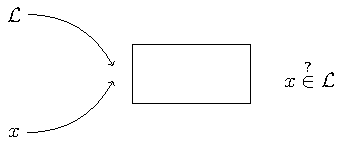
\includegraphics{./img/numerability/LanguageExample.pdf}
    \caption{Schematizzazione di un automa per un linguaggio $\Lang$}
\end{figure}

Come facciamo a dare al programma un input infinito? L'unico modo è fornire al programma una
descrizione finita dell'input. Creiamo quindi una struttura generativa finita che, da un insieme
finito di oggetti, ci permette di crearne dinamicamente di nuovi.

Questo esempio ci mostra come in questo ambito abbiamo un doppio livello di discussione:
\begin{itemize}

    \item uno descrittivo: a questo livello parlo di quello che mi serve per descrivere ciò di cui
    voglio parlare (e.g. la grammatica per un linguaggio). Vi sono una serie di problematiche legate
    a questo livello: la descrizione che do è giusta? È unica? Ce n'è una canonica? Ad esempio,
    date due grammatiche posso decidere se queste definiscono lo stesso linguaggio?

    \item uno denotazionale: a questo livello parlo veramente del mio oggetto in questione, a
    prescindere da qualsiasi descrizione se ne possa dare (e.g. un linguaggio). Abbiamo le stesse
    problematiche già viste per il livello descrittivo 

\end{itemize}

Il livello descrittivo è anche detto intensionale, quello denotazionale invece estensionale.

Anche per i programmi vale questa distinzione: la funzione calcolata da un programma fa parte del
livello denotazionale. Una funzione è descritta mediante il suo grafo. Non avendo modi diretti,
ovvero finiti, di descrivere la funzione usiamo un programma, che fa parte del livello descrittivo.
Una problematica interessante è la seguente: esiste una maniera di descrivere una funzione che non
mi dia anche un metodo effettivo per calcolarla (non un programma insomma)? 

Siamo costretti ad avere questi due tipi di livelli? Sì se l'oggetto di cui vogliamo parlare è
infinito. La comunicazione presuppone una descrizione finita dell'oggetto infinito.

Tutta la nostra intuizione è basata sul finito. Tuttavia molte cose che non valgono per il finito
valgono per l'infinito. Ad esempio è possibile mettere in corrispondenza biunivoca un sottoinsieme
stretto di un insieme infinito con l'insieme stesso, a differenza del caso finito. Questo è fuori
dalla nostra intuizione immediata degli insiemi.

A volte vogliamo fare ricerche infinite, e.g. su strutture dati infinite. Ad esempio potrei voler
verificare che una stringa $x$ appartenga ad un linguaggio $\Lang$ generando tutte le stringhe da
una grammatica per $\Lang$ e decidere ``Sì'' se $x$ compare. Ho un modo per dire se in una ricerca
troverò quello che cerco? In generale no. Questo problema è fondamentale perché è
frequentissimo. Parleremo in questi casi qui di semi-decisione. Notiamo inoltre che sul
complementare, ovvero $x \notin \Lang$, non possiamo dire niente.

Noi considereremo funzioni da $\Nat$ a $\Nat$ o, al massimo, da $\Nat^{k}$ a $\Nat$. Questo perché
i numeri naturali sono la più semplice struttura infinita. Questo non ci pone limitazioni di alcun
tipo. Se noi siamo interessati ad aspetti di calcolabilità tutto è alla fine riconducibile ad un
numero binario. Questa traduzione da un oggetto qualsiasi ad un numero naturale prende il nome di
Gödelizzazione. Ai tempi ($\sim 1930$) fu un'idea rivoluzionaria, ma dal punto di vista di un informatico
dovrebbe sembrare più naturale.

\section{Numerabilità}

Le seguenti sono note alle slide

\begin{defn}
    Un insieme $A$ si dice numerabile se esiste una funzione suriettiva $f$ dall'insieme
    dei numeri naturali $\Nat$ in $A$. $f$ è detta funzione di enumerazione.
\end{defn}

Un esempio di insieme numerabile è $\Nat$. Inoltre ogni sottoinsieme di un insieme numerabile è
ancora numerabile. La funzione $f$ ci dà anche un metodo di enumerazione degli elementi del
codominio di $f$.

\begin{lem}
   Sia $A$ numerabile. Allora $\set{*} \oplus A$ è ancora numerabile.
\end{lem}
\begin{proof}
    Sia $f : \Nat \to A$ la funzione di enumerazione di $A$. definiamo $g : \Nat \to \set{*} \oplus A$
    nel modo seguente:
    \begin{equation*}
        g(x) =
        \begin{cases}
            \case{g(0)=*}{}\\
            \case{g(x+1)=f(x)}{}\\
        \end{cases}
    \end{equation*}
    Chiaramente $g$ è suriettiva.
\end{proof}

Aggiungere un elemento non intacca la numerabilità di un insieme. Basta uno shift per avere una
nuova enumerazione di $A$. La numerabilità è resistente all'operazione di estensione.
\begin{cor}
    Sia $A$ numerabile e $D$ finito. Allora $D \oplus A$ è ancora numerabile.
\end{cor}

\begin{lem}
    L'unione di due insiemi numerabili $A$ e $B$ è ancora numerabile.
\end{lem}
\begin{proof}
    Siano $f$ e $g$ le due funzioni di enumerazione di $A$ e $B$. $A \oplus B$ è allora enumerato dalla seguente
    funzione $h$:
    \begin{equation*}
        h(x) =
        \begin{cases}
            \case{h(2x)=f(x)}{}\\
            \case{h(2x+1)=g(x)}{}\\
        \end{cases}
    \end{equation*}
\end{proof}

\begin{cor}
    Un unione finita di insiemi numerabili è numerabile.
\end{cor}
\begin{cor}
    Se $D$ è finito e $A$ è numerabile allora $D \times A$ è numerabile.
\end{cor}
\begin{proof}
    Per $A,B$ numerabili abbiamo $A \oplus B$ numerabile. Prendiamo in considerazione l'unione
    disgiunta di A con se stesso $k$ volte:
    \begin{equation*}
        \overbrace{\underset{0}{A} \oplus \underset{1}{A} \oplus \cdots \oplus
        \underset{k}{A}}^{\text{$k$ volte}}
    \end{equation*}
    Questo insieme è chiaramente numerabile. Chiamiamolo $A_{k}$. Abbiamo che:
    \begin{equation*}
        A_{k} = \bigcup_{i=0}^{k-1}\set{<i,a> \mid a \in A} = \set{<i,a> \mid a \in A, i \in
        \set{0,\dotsc,k-1}} = A \times K
    \end{equation*}
    da cui l'asserto.
\end{proof}

Possiamo enumerare $\Nat \times \Nat$? Vediamo com'è fatto questo insieme. Avremo $(0,0), (0,1),
(0,2),\dotsc$, dopodiché, sulla prossima riga, avremo $(1,0), (1,1), (1,2),\dotsc$, e così via
all'infinito. Il modo più conveniente per visualizzarlo è pensare a dei punti nel piano. 

Possiamo enumerarli? Sarebbe sbagliato numerare per righe o per colonne. Questo perché le righe e
le colonne sono infinite, iterando su una riga non passerò mai alla prossima. Che tecnica usiamo?
Dove tailing. Numeriamo per diagonali. Ce ne sono altre di numerazioni possibili. Va bene qualsiasi
``gioco dell'oca'' che passa per ogni coppia una e una sola volta.

\begin{figure}[h]
    \centering
    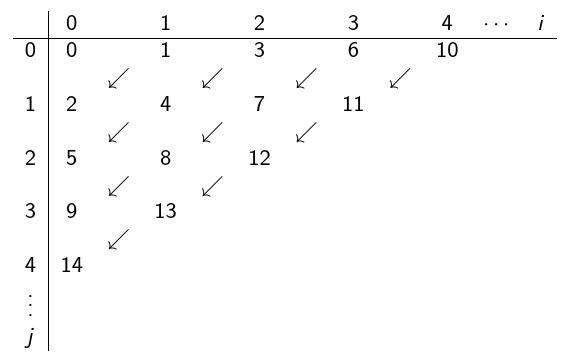
\includegraphics[scale=0.5]{./img/numerability/DoveTailing.jpg}
    \caption{Dove tailing}
\end{figure}

Questa codifica si ottiene nel seguente modo:
\begin{equation*}
    <i,j> = j + \sum_{k=0}^{i+j}k = \frac{(i+j)^{2}+i+3j}{2}
\end{equation*}
ed è giustificata dal ragionamento seguente: la somma delle componenti $i$ ed $j$ per i punti su di una
stessa diagonale è costante e pari al numero di diagonali già interamente percorse. Il numero di
punti del piano già visitati in queste diagonali è
\begin{equation*}
    \sum_{k=0}^{i+j}k = \frac{(i+j)(i+j+1)}{2}
\end{equation*}
Per visitare l'elemento $<i,j>$ dovrò ancora percorrere $j$ passi lungo l'ultima diagonale, da cui
la formula precedente.

Importante: Il dove tailing non è la diagonalizzazione.

Come corollario abbiamo che il prodotto cartesiano di due insiemi numerabili è numerabile.

È facile dimostrare che posso avere delle biezioni tra $\Nat^{k}$ e $\Nat$, in modo da codificare
delle tuple di numeri con un numero solo. In altre parole c'è una procedura algoritmica che mi
permette di passare da una tupla al corrispondente numero $n$ e da $n$ alla corrispondente tupla. Di
conseguenza $\Nat^{k}$, per $k$ naturale, è ancora numerabile.

\begin{lem}
    L'unione di un insieme numerabile di insiemi numerabili è ancora numerabile.
\end{lem}
\begin{proof}
    Sia $A$ un insieme numerabile e sia $f$ la sua funzione di enumerazione. Sia $\set{B_{a}\mid a
    \in A}$ una collezione di insiemi numerabili, ciascuno enumerato da una funzione $g_{a}$. La funzione
    $h : \Nat \times \Nat \to \bigcup_{a \in A}B_{a}$ definita da
    \begin{equation*}
        h(n,m) = g_{f(n)}(m)
    \end{equation*}
    è suriettiva.
\end{proof}

\begin{lem}
    Se $A$ è un insieme numerabile, anche $\bigcup_{i \in \Nat} A^{i}$ è numerabile.
\end{lem}

Consideriamo l'operatore di Kleene sull'alfabeto $\Sigma$: $\Sigma^{*}$. Anche questo insieme è
numerabile, perché è l'unione numerabile di insiemi numerabili (ricordiamo che $A^{k}$ è numerabile).

Un altro insieme numerabile interessante è l'insieme delle parti finite:
\begin{equation*}
    \Parts_{\textit{fin}}(\Nat) = \{A \mid A \subseteq \Nat, \textit{$A$  è finito}\}
\end{equation*}

Abbiamo due piani di infinità nei programmi: l'infinità dell'input e l'infinità del tempo di
calcolo, in quanto il mio programma può divergere su un dato input.

L'insieme di funzioni da $A$ a $B$ ha cardinalità $B^{A}$.

Possiamo caratterizzare l'insieme delle coppie su $A$, $A \times A = A^{2}$, come una funzione
dall'insieme $\BOOL = \{0,1\}$ all'insieme $A$. $f(x)$ può essere così definita: data
una coppia $<a_{1},a_{2}>$, $f(x)$: $ x \mapsto $ if $x$ then $a_{1}$ else $a_{2}$. Al posto dei booleani potremmo
avere un qualsiasi insieme di cardinalità 2.

$A^{K}$ è isomorfo all'insieme delle funzioni $f: K \to A$.

La funzione è utile sia come strumento di calcolo che come strumento di codifica dei dati.

Lo spazio delle funzioni da un insieme finito ad un insieme numerabile è ancora numerabile.

\section{Diagonalizzazione}

Consideriamo lo spazio delle funzioni da un insieme numerabile ad un altro insieme numerabile.
Ancora più semplicemente, possiamo considerare le funzioni da $\Nat$ a 2 (o $\BOOL$).

L'insieme delle funzioni da $A$ a $\BOOL$ è isomorfo all'insieme delle parti di $A$.

Per denotare un sottoinsieme si può dare una funzione caratteristica, che restituisce 1 se un
elemento fa parte del sottoinsieme e 0 altrimenti.

\begin{thm}
    Per ogni insieme $A$ non esiste una funzione suriettiva da $A$ in $\Parts(A)$.
\end{thm}
\begin{proof}
    Sia $f : A \to \Parts(A)$ una funzione suriettiva da $A$ all'insieme delle parti di $A$. Data
    $f$ posso costruire parametricamnente $\Delta_{f}$ così fatto:
    \begin{equation*}
        \Delta_{f} = \{a \mid a \in A, a \notin f(a)\}
    \end{equation*}
    Essendo $f$ suriettiva esiste $a$ tale che $f(a) = \Delta_{f}$. Ci chiediamo ora, $a \in f(a)$?
    \begin{equation*}
        a \in f(a) \iff a \in \Delta_{f} \iff a \in A \land a \notin f(a)
    \end{equation*}
    Ma questo è assurdo.
\end{proof}

La tecnica con cui si dimostra questo teorema è detta tecnica diagonale, o diagonalizzazione.
Un'idea intuitiva che giustifica il nome è la seguente: consideriamo una tabella indicizzata per
colonne dagli $a \in A$ e sulle righe dagli $f(a)$ per ogni $a \in A$. Nella cella $(i,j)$ della
tabella avrò 1 se $a_{j} \in f(a_{i})$ e 0 altrimenti. Abbiamo per ogni riga la funzione
caratteristica di $f(a)$, per ogni $a \in A$. Abbiamo ora che la funzione caratteristica di
$\Delta_{f}$ è costruita andando sulla diagonale e prendendo l'elemento $j$ in $\Delta$ se in
corrispondenza sulla diagonale, ovvero alla riga $i$, ho 0, lasciandolo fuori altrimenti. Di
conseguenza la funzione caratteristica che vado a costruire per definire $\Delta$ è diversa da
tutte le funzioni caratteristiche sulle righe almeno per un elemento.

La diagonalizzazione è un metodo semplice per creare un nuovo elemento diverso da tutti quelli di
una lista sotto certe ipotesi.

Dimostriamo che i numeri nell'intervallo $[0,1[$ sono una quantità non numerabile. Come possiamo
descrivere i numeri reali? Possiamo farlo, ad esempio, con la loro rappresentazione decimale: una
infinita successione delle cifre del numero, per ogni numero.

Supponiamo di avere una enumerazione dei numeri reali $r_{0}, r_{1}, r_{2}, \dotsc$. Disegnamo una
tabella con le righe indicizzate dai numeri reali nell'ordine dato dall'enumerazione e con le
colonne indicizzate dai numeri naturali. Per ogni numero della enumerazione possiamo scrivere, in
corrispondenza della colonna $j$, la sua cifra $j$, in ordine da sinistra verso destra. 

Consideriamo la diagonale della tabella. Consideriamo il mapping che per gli elementi dell'insieme
$\{0,\dotsc,4\}$ restituisce 7 mentre per gli elementi dell'insieme $\{5,\dotsc,9\}$ restituisce 3.
Se prendiamo la diagonale e alle sue cifre applichiamo il mapping creato otteniamo un numero che è
diverso da tutti gli elementi dell'enumerazione almeno per la cifra sulla diagonale. Di conseguenza
non fa parte dell'enumerazione. Ma questo è assurdo, dato che avevo supposto di poter enumerare
tutti i numeri reali dell'intervallo $[0,1[$.

Le funzioni da $\Nat$ a 2, a $\{0,\dotsc,9\}$, a $\Nat$ hanno la stessa cardinalità, quella del
continuo, che non è numerabile.

Esistono quindi numeri reali per i quali non esiste una maniera per descriverli.

\section{Definibilità vs. Calcolabilità}

Le funzioni da $\Nat$ a $\Nat$ di cui possiamo parlare hanno cardinalità numerabile. Anche i programmi sono
una quantità numerabile.

Non è però questo il problema che vogliamo affrontare. È evidente per ragioni di cardinalità che
ci sono funzioni che non potremo calcolare. Il problema a cui siamo interessati è: tutte le
funzioni che possiamo definire sono calcolabili o ci sono funzioni definibili ma non calcolabili?

Abbiamo inizialmente il problema di cosa significa definibile. La nozione di definibilità dipende
dal contesto e dal potere espressivo del linguaggio che uso (e.g. linguaggio dell'aritmetica, linguaggio
del secondo ordine, ecc.).

Possiamo formalizzare la nozione di definibilità? No. È possibile dimostrare che l'idea di
definibilità non è definibile. Non è possibile dire quando una cosa è ben definita.

Supponiamo di avere un criterio che scansiona le stringhe e decide se una è una buona definizione o
no. Possiamo quindi definire una sequenza di funzioni e quindi dare una numerazione delle funzioni
definibili. Si può dimostrare che questa definizione di definibilità è incompleta, non cattura
bene il nostro senso intuitivo di definibilità. 

Intuitivamente, possiamo creare una tabella con le righe indicizzate dalle funzioni definite e per
colonne dai numeri naturali. La casella $(i,j)$ contiene il risultato della funzione $f_i$ sul
numero $j$. Supponiamo inoltre di avere funzioni binarie, ovvero che restituiscono 1 o 0. Questa
semplificazione non fa perdere di generalità. 

Con un procedimento diagonale possiamo definire una nuova funzione che non sta nell'enumerazione. Ad
esempio, sia $f(n) = 1 - d_{n}(n)$. Se questa definizione intuitivamente valida non è presente
nell'enumerazione allora il mio criterio è incompleto.  Supponiamo che nella mia enumerazione la
mia funzione $f$ compaia in posizione $m$. Allora avremmo $d_m(m) = f(m) = 1 - d_m(m)$. Ma questo è
assurdo.

Se fissiamo un linguaggio l'insieme delle funzioni definite su quel linguaggio è numerabile. Esiste
quindi una funzione, per quel linguaggio, che mi dica se una definizione è valida. Questa funzione,
tuttavia, non è calcolabile.

\subsection{Paradosso di Russel}

Questo è un vero paradosso, che mise in crisi la matematica agli inizi del XX secolo.

Possiamo pensare ad un insieme come ad una collezione di cose che rispetta certe proprietà. Data
una proprietà $P(x)$ possiamo costruire un insieme che la rispetti:
\begin{equation*}
    \frac{P(t)}{t \in \{x \mid P(x)\}} % the proving package may be useful here
\end{equation*}
Vale anche l'implicazione inversa

Pensiamo alla proprietà $P(x) = ``x \notin x''$. Possiamo costruire l'insieme $U = \{x \mid x \notin x\}$. Ci
chiediamo ora: $U \in U$? Abbiamo che $U \in U \iff U \notin U$. Ma questo è paradossale.

Il problema è che all'inizio del secolo si era tentato di basare la teoria insiemistica sul
principio di comprensione. Per quanto comodo e bello questo, nella forma che abbiamo visto, è causa
di paradossi. Dobbiamo rinunciare all'idea che basti pensare ad una proprietà per poter creare un
insieme che la rispetti.

\subsection{Paradosso di Berry}

%Berry era un bibiliotecario che si era appassionato un pò di matematica. // curiosità storiche
C'è un principio importante nei numeri naturali che dice che dato un sottoinsieme finito dei numeri
naturali esiste un elemento dei naturali che è il più piccolo numero naturale che non appartiene a
questo sottoinsieme.

Supponiamo di definire i numeri con stringhe di lunghezza $d$. Abbiamo quindi un insieme di numeri
che posso definire con al più $d$ caratteri. Possiamo definire $n_d$ come il più piccolo numero
non definibile con meno di $d$ caratteri, e sappiamo che esiste per il principio precedentemente
riportato.

Prendiamo ad esempio $d=100$. Abbiamo che $n_{100}$ non è definibile con meno di 100 caratteri. Eppure
è definito dalla stringa: ``$n_{100}$ non è definibile con meno di 100 caratteri'', che ha meno di 100
caratteri. Questo è assurdo.

%Più formalmente, supponiamo che la definizione sia data dalla stringa $s$ e prendiamo $d_{s} = |s| +
%1$. $n_{d_{s}}$ è il più piccolo numero non definibile con meno di $d_{s}$ caratteri. Ma
%$n_{d_{s}}$ è definito da $s$. Assurdo. // Non mi sembra corretta

Ci sono paradossi e paradossi. Alcune sono cose che sembrano strane ma in realtà non lo sono così
tanto. Altri sono proprio cattivi, mettono in questione aspetti fondamentali della nostra
intuizione.

Dove sta il problema del paradosso di Berry? Nella stringa $s$, perché la nozione di definibilità non
è definibile, ed $s$ la usa. La definizione data non è una buona definizione.

Ci chiediamo: data una enumerazione $\theta$ delle sentenze dell'aritmetica è possibile generare una
formula che mi dice il valore di verità di una sentenza dell'enumerazione?

Ad ogni sentenza dell'enumerazione associamo un numero, detto di Gödel. Questo perché non possiamo
parlare delle sentenze in sè in aritmetica, ma possiamo parlare solo di numeri. Quindi ci serve un
numero per parlare della sentenza.

La verità è intesa sul modello dei numeri naturali.

Vogliamo una formula \textit{Vera} tale che
\begin{equation*}
    \StdNat \models A \iff \StdNat \models \textit{Vera}(g(A))
\end{equation*}
dove $g(A)$ rappresenta il numero di Gödel di $A$.

Per i numeri naturali c'è un lemma detto lemma di diagonalizzazioe. Questo dice che dato un
predicato è sempre possibile trovare una formula $S$ tale che $\StdNat \models S \iff \StdNat \models
P(g(S))$. È possibile, per una sentenza, dire "quel predicato P vale per me". La dimostrazione è
interessante perché costruttiva.

Prendiamo come $P(x)$ la formula $\lnot \textit{Vero}(x): \StdNat \models P(x) \iff \StdNat \models
\lnot \textit{Vero}(x)$. Possiamo allora costruire $S$ tale che $\StdNat \models S \iff \StdNat
\models \lnot Vero (S)$. Avremmo quindi $\StdNat \models S \iff \StdNat \models \lnot S$. Ma questo è
paradossale.  Quindi non è definibile, nel linguaggio dell'aritmetica, una formula che, data una
sentenza dell'aritmetica, mi dice se questa è vera, in senso aritmetico. Questo risultato è
soprendentemente forte e va sotto il nome di teorema di Tarski.

Un'idea simile viene usata nel teorema di Gödel non con la nozione di verità matematica ma con la
nozione di dimostrabilità. Il risultato è che la formula che afferma la propria indimostrabilità
non è dimostrabile. Da ciò il sistema logico è incompleto, ovvero c'è una formula indimostrabile.

\chapter{Il formalismo primitivo ricorsivo}

\section{Ricorsione primitiva}

Nei linguaggi di programmazione siamo abituati all'autoreferenzialità, o ricorsione. In generale
bisogna fare attenzione.

Esistono forme esplicite ed implicite di autoreferenziazione. Per le seconde ho un oggetto che ha
una sezione universale nel suo scope e tale che l'oggetto stesso ci rientra. È una sorta di ordine
superiore.

Ad esempio:
\begin{quote}
    ``Tutte le sentenze universali sono false''
\end{quote}

Questa frase è implicitamente autoreferenziale. Nel suo raggio di applicabilità include se stessa.

Per le formule aperte non ha senso parlare di verità. Si può parlare solo di verità in caso di
formule chiuse, ovvero sentenze. I teoremi sono tutti chiusi. La sentenza sopra è dimostrabilmente falsa.

Ci chiediamo se la definibilità di una funzione implichi la sua calcolabilità e anche se vale il 
viceversa. Sappiamo già che la nozione di definibilità è legata al linguaggio che utilizzo.

Possiamo dare una definizione precisa di calcolabilità? È una problematica delicata, legata al
sistema di calcolo che utilizzo e alla definizione formale di algoritmo, che non è banale.

%// TODO DEVE STARE PROPRIO QUA QUESTA AFFERMAZIONE?
%È facile dimostrare che il while è più espressivo del for dato che è possibile implementare il
%for con un while.

Ci chiediamo, vogliamo davvero avere un loop infinito? In certi casi sì, ad esempio per stampare
una lista di numeri primi ed interromperla quando voglio. Ma non è comune, molto spesso ci basta
una iterazione determinata.

Le funzioni dell'informatica sono di una categoria particolare: sono funzioni parziali. Le funzioni
totali calcolabili sono un sottoinsieme delle funzioni parziali.

Ci poniamo il problema di giustificare l'inclusione, nei nostri linguaggi di programmazione, di
costrutti che possono causare divergenza. Hanno un'utilità che giustifica il rischio di non
terminazione dei programmi.

Noi siamo abituati a scrivere funzioni ricorsive. Ad esempio, $\textit{Fact}(n+1) =
(n+1)*\textit{Fact}(n)$, assieme al caso base. Dal punto di vista matematico questo oggetto è
strano. Non si può definire una cosa in funzione di se stessa. C'è modo di definire in una maniera
più sensata a livello matematico una funzione ricorsiva, che sottintende una procedura? È una
problematica interessante.

La ricorsione primitiva è un tipo di ricorsione simile a quella finora vista ma con dei limiti
semantici. In particolare possiamo dare il vincolo: nel corpo della definizione di $f(n+1)$ ci si
può richiamare ricorsivamente solo su $n$.  È equivalente limitare le chiamate ricorsive a oggetti
più piccoli di $n+1$.
%È equivalente ma più debole, dal punto di vista dell'espressività, limitare le chiamate ricorsive a
%oggetti più piccoli di $n+1$. // ?? Equivalente ma piu' debole?

La ricorsione primitiva, per vincoli strutturali, garantisce la terminazione. Siamo interessati a
questa classe di funzioni perché c'è un teorema che dice che le funzioni definibili in questo modo
sono esattamente quelle definibili con un for.

Prendiamo come primitive alcune funzioni nel nostro linguaggio primitivo ricorsivo $\Lang$:
\begin{enumerate}
    \item le funzioni costanti:
        \begin{equation*}
            c^{k}_{m}(x_{1},x_{2},\dotsc,x_{k}) = m \quad \text{$m$ in $\Nat$}
        \end{equation*}
    \item le proiezioni:
        \begin{equation*}
            \pi_{i}^{k}(x_{1},x_{2},\dotsc,x_{k}) = x_{i} \quad \text{per qualche $1 \leq i \leq k$}
        \end{equation*}
    \item la funzione successore:
        \begin{equation*}
            s(x) = x + 1
        \end{equation*}
\end{enumerate}

Ammettiamo inoltre due schemi composizionali per definire nuove funzioni a partire da quelle già
esistenti:
\begin{enumerate}
    \item Composizione: se $h : \Nat^{n} \to \Nat$ e $g_{1},g_{2},\dotsc,g_{n}:\Nat^{k} \to \Nat$
    appartengono a $\Lang$, anche la funzione $f: \Nat^{k} \to \Nat$ così definita:
    \begin{equation*}
        f(\vec{x}) = h(g_{1}(\vec{x}),g_{2}(\vec{x}),\dotsc,g_{n}(\vec{x}))
    \end{equation*}
    appartiene a $\Lang$, con $\vec{x} = (x_{1},x_{2},\dotsc,x_{k})$.
    \item Ricorsione primitiva: se $g: \Nat^{k} \to \Nat$,$h: \Nat^{k+2}\to \Nat$ appartengono a
    $\Lang$, allora che $f: \Nat^{k+1} \to \Nat$, così definita:
    \begin{equation*}
        f(n,\vec{x}) =
        \begin{cases}
            \case{f(0,\vec{x}) = g(\vec{x})}{}\\
            \case{f(y+1,\vec{x}) = h(y,f(y,\vec{x}),\vec{x})}{}\\
        \end{cases}
    \end{equation*}
    appartiene a $\Lang$, con $\vec{x} = (x_{1},x_{2},\dotsc,x_{k})$.
\end{enumerate}

Quando ho più strade di espansione nei sistemi di riscrittura il problema di capire se la strada
che scelgo è influente è il problema della confluenza, legato alla terminazione dell'espansione.

Nell'esecuzione ci sono dei problemi che non abbiamo indicato esplicitamente, come la valutazione
per valore e per nome, l'ordine di valutazione delle espressioni, i side effect, ecc.

%Non è chiaro cosa calcoli la funzione. È possibile semplificare il codice mediante inlining.

L'idea delle funzioni ricorsive primitive è che abbiamo un argomento su cui facciamo la ricorsione
ed una serie di parametri aggiuntivi.

Lavorare su una ``sottostruttura'' dell'input in ricorsione garantisce la terminazione della chiamata.
La ricorsione primitiva è un sottocaso della ricorsione strutturale. Con la seconda ci si richiama
solo su sottostrutture strette.

\subsection{Esempi di funzioni primitive ricorsive}

Vediamo ora alcuni esempi di definizioni di funzioni comuni nel formalismo primitivo ricorsivo.

\begin{equation*}
    \textit{add}(x,y) = 
    \begin{cases}
        \textit{add}(0,y) = y \\
        \textit{add}(x+1,y) = \textit{succ}(\textit{add}(x,y))
    \end{cases}
\end{equation*}

\begin{equation*}
    \textit{mult}(x,y) = 
    \begin{cases}
        \textit{mult}(0,y) = 0 \\
        \textit{mult}(x+1,y) = \textit{add}(\textit{mult}(x,y),y)
    \end{cases}
\end{equation*}

Il meccanismo della definizione di funzioni per ricorsione primitiva è naturale. Molte funzioni
sono strutturate in maniera ricorsiva.

\begin{equation*}
    \textit{fact}(x) =
    \begin{cases}
        \textit{fact}(0) = 1 \\
        \textit{fact}(x+1) = (x+1)*\textit{fact}(x)
    \end{cases}
\end{equation*}

%La calcolabilità la definiamo sui numeri naturali, interi positivi.
%Per la differenza fai un preambolo del tipo "Vediamo due definizioni della funzione sub, una
%sbagliata ..."

La seguente funzione mi restituisce 1 se l'input è 0 e 0 altrimenti.
\begin{equation*}
    \textit{test}(x) = 
    \begin{cases}
        \textit{test}(0) = 1 \\
        \textit{test}(x+1) = 0
    \end{cases}
\end{equation*}

Proviamo a definire la funzione differenza. Ricordiamo che abbiamo definito la calcolabilità sui
numeri naturali, interi positivi. Di conseguenza non possiamo calcolare la differenza, ad esempio,
tra 3 e 7. Noi vogliamo una funzione che calcoli $a - b$ se $a > b$. In tutti gli altri casi
calcoliamo 0.

Una prima definizione naïve di $a - b$ è la seguente:
\begin{equation*}
    \textit{sub}(a,b) =
    \begin{cases}
        \textit{sub}(0,b) = 0 \\
        \textit{sub}(a+1,b) = \textit{succ}(\textit{sub}(a,b))
    \end{cases}
\end{equation*}

Questa è sbagliata rispetto alla nostra specifica. Per $sub(1,1)$, ad esempio, restituisce 1. Una
scelta migliore sarebbe andare in ricorsione su b.

Una delle scelte da fare è su cosa andare in ricorsione. Può essere uno dei parametri oppure un
nuovo valore costruito a partire dai parametri.

Proviamo con la seguente definizione:
\begin{equation*}
    \textit{sub}(a,b) =
    \begin{cases}
        \textit{sub}(a,0) = a \\
        \textit{sub}(a,b+1) = \textit{pred}(\textit{sub}(a,b))
    \end{cases}
\end{equation*}
dove \textit{pred} restituisce 0 per 0 e $x-1$ in ogni altro caso.

Questa definizione è un pò borderline, perché andrebbe dimostrato che cambiando il parametro su
cui vado in ricorsione ottengo un formalismo equivalente a quello introdotto. Tuttavia ciò è
possibile perciò la definizione rientra nel formalismo primitivo ricorsivo.

Vogliamo ora una funzione che restituisca 1 se i parametri sono uguali, 0 altrimenti.

\begin{equation*}
    \textit{comp}(n,m) = test(\textit{add}(\textit{sub}(n,m),\textit{sub}(m,n)))
\end{equation*}

Benchè sembri limitante è veramente potente questo tipo di ricorsione.

Quando parliamo di predicati intendiamo funzioni che restituiscano un booleano.

Supponiamo di saper calcolare un certo predicato $P$. Possiamo calcolare anche la sua negazione.

Data la funzione caratteristica di $P$, $c_{P}$, possiamo calcolare la funzione caratteristica di
$\comp{P}$: $c_{\comp{P}}(x) = 1 - c_{P}(x)$.

Date $c_{P}$ e $c_{Q}$ abbiamo che $c_{P \land Q}(x) = c_{P}(x) *
c_{Q}(x)$.

È possibile definire $c_{P \lor Q}$ con le leggi di de Morgan: $A \lor B = \comp{\comp{A \lor B}} =
\comp{\comp{A} \land \comp{B}}$. Un altro modo è usano la funzione normalizzazione, che normalizza i
numeri a 0 e 1:
\begin{equation*}
    c_{P \lor Q}(x) = \textit{norm}(c_{P}(x) + c_{Q}(x))
\end{equation*}

Dati dei predicati possiamo quindi calcolare i connettivi logici tra di loro nel nostro formalismo.
Passiamo ora al discorso dei quantificatori.

Per calcolare il quantificatore esistenziale dovrei avere una procedura del genere:

% python listing?
\begin{python}
x = 0
while $\lnot P(x)$:
    x = x + 1
\end{python}

Questo potrebbe ciclare all'inifinito se l'esiste non vale. Abbiamo un problema duale con il
quantificatore universale.

È evidente che c'è un problema ma non è detto che questo non sia insormontabile.

Quello che sappiamo senza dubbio calcolare è la quantificazione limitata, o bound. L'idea è che
ho un upper bound finito alla mia quantificazione. Calcoleremmo quindi $g(n) = \exists x \leq n,
P(x)$.

Ovviamente possiamo calcolare la quantificazione limitata con la ricorsione primitiva. Nel caso del
quantificatore universale:

\begin{align*}
    f(0) &= P(0) \\
    f(n+1) &= P(n+1)*f(n)
\end{align*}

Tanti problemi aperti dell'aritmetica sono legati alla quantificazione: sapere se esiste un numero
che ripetti tale proprietà o se una tale proprietà vale per tutti i numeri.

È anche una maniera per approcciarsi ai problemi. Domandarsi se c'è un bound permette di rendere
l'algoritmo più efficiente e certamente terminante.

\section{Test di primalità}

Vediamo ora un altro predicato interessante, il test di primalità.

Perché escludiamo 1 dai numeri primi? Perché uno dei risultati più importanti dell'aritmetica è
la fattorizzazione unica, che vale per tutti i numeri escludendo 1. Per mantenere quel teorema 1
viene escluso.

Definiamo la proprietà $P(x)$:

\begin{equation*}
    x > 1 \land \forall z (z | x \implies (z = 1 \lor z = x))
\end{equation*}

$z | x$ è notazione per $z$ divide $x$ (più precisamente, $z$ è un fattore di $x$).

\begin{equation*}
    z | x := \exists a, z * a = x := \exists a \leq x, z * a = x
\end{equation*}

Possiamo porre un bound anche al test di primalità: possiamo fermarci ad $x$. Siamo quindi in grado di
definire (e calcolare) il test di primalità.

\section{Minimizzazione}

Vediamo ora un'altra operazione che opera su domini limitati che useremo molto spesso: la
minimiazzazione.

\begin{equation*}
    \mu x, P(x)
\end{equation*}

Possiamo vederla come uno snippet del genere:

\begin{python}
x = 0
while $\lnot P(x)$:
    x = x + 1
return x
\end{python}

Fissiamo un ordinamento e cerchiamo il primo $x$ che soddisfa $P(x)$. Quello che ci interessa alla fine
del ciclo è il valore di $x$. Questo è, sostanzialmente, cosa l'operazione di minimizzazione fa.

While è un costrutto imperativo. Noi preferiamo, per la nostra teoria della calcolabilità, un
costrutto funzionale, da cui l'introduzione del $\mu$. Il risultato di questo operatore è $x$.

Al solito col while abbiamo il problema che il while potrebbe non fermarsi mai. Quello che possiamo
certamente sperare di scrivere, e quindi calcolare, nel nostro formalismo è una forma limitata di
$\mu$. Cerchiamo il più piccolo $x$ minore di un certo $y$ su cui vale un predicato $P(x,\vec{z})$.

\begin{equation*}
    f(y,\vec{z}) = \mu x \leq y, P(x,\vec{z})
\end{equation*}

I parametri di $\vec{z}$ rappresentano parametri ulteriori che possono essere utili.

Cosa vogliamo restituire se non troviamo $x$ nell'intervallo fissato? Dobbiamo restituire un valore
e ne possiamo restituire uno qualunque. La cosa più naturale è restituire $y + 1$, se $y$ è il
mio upper bound.

Vogliamo trovare un modo per scrivere questa operazione, non necessariamente per calcolarla
efficientemente.

Definiamo prima il predicato $R$:
\begin{equation*}
    R(y,\vec{z}) = \forall x \leq y, \lnot P(x,\vec{z})
\end{equation*}

Questo mi dice ``fino a $y$ non ho trovato il minimo'', con $y$ compreso.

$R$, come funzione, è una costante di valore 1 fino all'$y_{0}$ minimo per cui vale
$P(y_{0},\vec{z})$. Da lì in poi il suo valore diventa costantemente 0.

Possiamo ora scrivere $\mu x$:

\begin{equation*}
    \mu x \leq y, P(x,\vec{z}) = \sum_{w \leq y}\lnot R(w,\vec{z})
\end{equation*}

Possiamo definirlo in un altro modo. Prendiamo in considerazione il predicato $M$:

\begin{equation*}
    M(x,\vec{z}) = P(x,\vec{z}) \land \forall y < x, \lnot P(y,\vec{z})
\end{equation*}

Questo predicato mi dice ``$x$ è il più piccolo valore per cui vale $P$''. Come faccio però a trovare
$x$? Si può moltiplicare $x$ per $M(x,\vec{z})$. Dato che dobbiamo testare tutti gli $x \leq y$, abbiamo
che $\mu$ può essere espresso come:
\begin{equation*}
    \mu x \leq y, P(x,\vec{z}) = \sum_{x \leq y} x \cdot M(x,\vec{z})
\end{equation*}

\section{Generazione numeri primi}

Come possiamo trovare il più piccolo numero primo successivo ad un numero $i$? Con la seguente
funzione, ad esempio:
\begin{equation*}
    \Pi(i) = 
    \begin{cases}
        \Pi(0) = 2 \\
        \Pi(x + 1) = \mu p. \textit{prime}(p) \land p > \Pi(x)
    \end{cases}
\end{equation*}

Cosa manca? Bisogna dare un bound alla minimizzazione. C'è un teorema che dice che è sempre
possibile trovare un numero primo tra $n$ e $2n$. Il bound che possiamo dare è $2\Pi(x)$.

L'importante è dare un bound. C'è un altro bound, molto più grande, che andrebbe bene comunque:
$\Pi(x)!$.

Come si dimostra l'infinità dei numeri primi? Supponiamo che siano finiti e siano $p_{1}, p_{2},
\dotsc, p_{n}$. Prendiamo il numero $p_{1}\cdot p_{2}\cdots p_{n} + 1$. Questo numero non è
divisibile per nessun $p_{i}$ della mia enumerazione. Quindi o è un numero primo oppure i suoi
fattori non fanno parte di quella lista. In ogni caso ho un assurdo.

È una dimostrazione bella. La tecnica è analoga alla diagonalizzazione: costruisco un nuovo
elemento da quelli di una lista che prova il mio assurdo.

\section{Ricorsione multipla}

Consideriamo una possibile codifica del piano e consideriamo la coppia $<n,m>$. Non siamo troppo
interessati alla codifica della coppia in sè, ma alle funzioni che mi restituiscono le componenti
della coppia.

Abbiamo che, in generale, le componenti sono $\leq$ della (codifica della) coppia: $n \leq <n,m>$ e
$m \leq <n,m>$.

Supponiamo di voler calcolare $\pi_{1}(x)$, ovvero la prima proiezione della coppia $x$. Partiamo
dalla seguente definizione:
\begin{equation*}
    \pi_{1}(x) = \mu n, \exists m, <n,m> = x
\end{equation*}

Manca un bound. Quale prendiamo? $x$:

\begin{equation*}
    \pi_{1}(x) = \mu n \leq x, \exists m \leq x, <n,m> = x
\end{equation*}

Talvolta la ricorsione può essere necessaria su più di un valore. Nel formalismo che abbiamo visto
finora non abbiamo questa possibilità.

Consideriamo la sequenza di Fibonacci:
\begin{align*}
    \textit{fib}(0) &= 1 \\
    \textit{fib}(1) &= 1 \\
    \textit{fib}(x+2) &= \textit{fib}(x+1) + \textit{fib}(x)
\end{align*}

La funzione di Fibonacci è intrinsicamente esponenziale, ma questo è il peggior metodo per
calcolarlo. Siamo esponenziali nel numero di chiamate oltre ad esserlo nell'input. Inoltre così
com'e scritta ora non rispetta i vincoli del formalismo primitivo ricorsivo.

Qual è l'idea? Bisogna portarsi dietro un accumulatore.

Vogliamo definire la seguente funzione:
\begin{equation*}
    \textit{fibo'}(x) = <\textit{fib}(x),\textit{fib}(x+1)>
\end{equation*}

Possiamo definirla nel formalismo primitivo ricosivo nel seguente modo:
\begin{align*}
    \textit{fibo'}(0) &= <1,1> \\
    \textit{fibo'}(x+1) &= <\textit{fib}(x+1),\textit{fib}(x+2)> \\
    &= <\pi_{2}(\textit{fibo'}(x)),\pi_{1}(\textit{fibo'}(x)) + \pi_{2}(\textit{fibo'}(x))>
\end{align*}

L'unica chiamata ricorsiva che faccio è $\textit{fibo'}(x)$.

Questa funzione corrisponde all'incirca al seguente snippet:
 
\begin{python}
$acc_{0}$ = 1
$acc_{1}$ = 1 
for $i$ in range(x+1):
    tmp = $acc_{0}$
    $acc_{0}$ = $acc_{1}$
    $acc_{1}$ = tmp + $acc_{1}$
return $acc_{1}$
\end{python}

Questa tecnica è generale è prende il nome di ricorsione di coda.

Tutte le funzioni ricorsive primitive possono essere espresse mediante un for. È possibile
dimostrare anche il viceversa. Il formalismo primitivo ricorsivo è equivalente, a potere
espressivo, ai programmi scrivibili con il for, ovvero senza while e senza ricorsione generale.

\section{Funzione di Ackermann}

Vediamo ora una funzione che non è possibile scrivere nel formalismo primitivo ricorsivo. Va
immaginata come una famiglia di funzioni dove il primo parametro mi istanza la particolare funzione.
Abbiamo $\textit{ack}_{0}$, $\textit{ack}_{1}$, etc.

\begin{align*}
    \textit{ack}(0, 0, y ) &= y\\
    \textit{ack}(0, x + 1, y ) &= \textit{ack}(0, x, y ) + 1\\
    \textit{ack}(1, 0, y ) &= 0\\
    \textit{ack}(z + 2, 0, y ) &= 1\\
    \textit{ack}(z + 1, x + 1, y ) &= \textit{ack}(z, \textit{ack}(z + 1, x, y ), y )
\end{align*}

I casi sono mutalmente disgiunti. Data una tripla qualsiasi di valori solo una riga si applica.

La funzione termina? Sì, ma non è banale. L'argomento più importante della funzione è il primo.
Se il primo decresce bene. Altrimenti vado a vedere gli altri. Questo mi dà un ordinamento delle
mie chiamate ricorsive che mi da un'idea del fatto che la funzione è terminante.

Cosa calcola? $\textit{ack}_{0}$ è abbastanza banale: è la somma. $\textit{ack}_{1}$ invece
calcola il prodotto tra $x$ e $y$. $\textit{ack}_{2}$ calcola l'elevamento a potenza ($y^x$).

$\textit{ack}_{i}$ itera $\textit{ack}_{i-1}$. Il prodotto itera la somma. L'elevamento a potenza
itera la moltiplicazione la tetrazione itera l'elevamento a potenza.

La funzione, benchè terminante, ha una complessità spaventosa.

Perché non posso scriverla nel formalismo primitivo ricorsivo? Perché questa funzione cresce
troppo velocemente. Cresce più velocemente di qualsiasi funzione esprimibile col formalismo
primitivo ricorsivo. La funzione di Ackermann mi dà un bound computazionale alle funzioni
esprimibili con il formalismo primitivo ricorsivo. Di conseguenza non può essere esprimibile nello
stesso formalismo.

Se riesco ad esprimere un bound computazionale alla complessità di un programma so che non è
possibile calcolare quel bound nello stesso formalismo in cui ho espresso il mio programma.

Tutte le singole istanze di Ackermann sono scrivibili nel formalismo primitivo. Ma non posso
scrivere un programma che le esprima tutte. Il formalismo non è abbastanza parametrico.

È sufficiente  aggiungere l'ordine superiore al formalismo primitivo per poter esprimere la
funzione di Ackermann.

La funzione di Ackermann è una funzione chiaramente calcolabile, essendo esprimibile in un qualche
linguaggio di programmazione, ma non è esprimibile nel formalismo primitivo ricorsivo.

Si può dimostrare che c'è un ordinamento ben fondato e quando facciamo le chiamate ricorsive nella
funzione di Ackermann le variabili decrescono secondo questo ordine.

Un ordinamento si dice ben fondato se non esistono catene discendenti infinite.

Dire che ho un ordinamento ben fondato non è la stessa cosa di dire che di elementi minori di un
dato elemento $m$ ce ne sono una quantità finita.

Vediamo un esempio: l'ordinamento lessicografico. Considerando $\Nat \times \Nat$. Definiamo
l'ordinamento $<_{p}$ nel seguente modo: $<n_{1},m_{1}> <_{p} <n_{2},m_{2}> \iff n_{1} < n_{2} \lor
(n_{1} = n_{2} \land m_{1} < m_{2})$. Questo ordinamento è ben fondato. Vale che $\forall m, <2,m>
<_{p} <3,7>$.

Non è possibile costruire catene discendenti infinite. Proviamo a costruirne una:
$<3,7> >_{p} <3,6> ... <3,0> >_{p} <2,10^{4}>$

Arrivati qui posso ripetere il giochetto di prima finché non arrivo a 0, dopodiché dovrò
decrementare la prima componente. Di queste sequenze ne posso fare di lunghezza arbitraria ma sempre
finita. Questo ragionamento ci dà un'idea del perché la funzione di Ackermann termina (il
principio alla base della dimostrazione è lo stesso).

\chapter{Altri formalisimi e Macchine di Turing}

\section{Formalismi totali e problema dell'interprete}

Ci sono varie estensioni possibili al formalismo primitivo ricorsivo. Un esempio è il sistema T di
Gödel, che aggiunge l'ordine superiore. Questo ci permette di scrivere la funzione di Ackermann.
Un'altra possibilità è quella di rilassare la ricorsione primitiva permettendo una ricorsione che
permetta di andare in ricorsione su ordinamenti ben fondati. Questa condizione è verificabile in
termini sintattici, entro certi limiti.

Esteso il mio linguaggio ottengo la possibilità di scrivere la funzione di Ackermann e le mie
funzioni sono totali. Sono complete? O c'è qualche funzione totale che posso pensare ma non
scrivere? C'è una dimostrazione che dice che sì, tutti questi formalismi saranno incompleti. Un
formalismo che permette di scrivere solo programmi terminanti sarà sempre incompleto.

La dimostrazione è abbastanza semplice. L'idea è che un programma che non riesco a scrivere (tra
i tanti) è l'interprete per il linguaggio stesso. 

Cosa intendiamo per interprete? Qui parliamo sempre di funzioni da $\Nat$ a $\Nat$. Dovremmo quindi
definire l'interprete in questi termini.

L'input dell'interprete non è un programma in senso astratto. Prende in input una stringa che
esprime il programma. Questa stringa può essere letta come un numero. Dire che una funzione è
calcolabile è equivalente a definire l'interprete per tale funzione, se vogliamo dare una
definizione operativa.

Sia data una enumerazione effettiva (e.g. lessicografica) $P_{n}$ dei programmi del
linguaggio $\Lang$, e sia $\phi_{n}$ la funzione calcolata dal programma $P_{n}$.

$P_{n}$ è un livello intensionale, una descrizione di una funzione. $\phi_{n}$ è la funzione
calcolata dal programma $n$-esimo.

Un interprete per $\Lang$ `e una funzione che preso in input l'indice $n$ di un programma ed un
input $m$ simula il comportamento di $P_{n}$ su tale input, cio`e una funzione $I$ tale che
\begin{equation*}
    I (n, m) = \phi_{n}(m)
\end{equation*}

Se la numerazione dei programmi `e effettiva, $I$ `e intuitivamente calcolabile.

È fondamentale la numerazione: dato $n$ devo poter sapere qual'è la funzione $n$-esima da interpretare.

Ci chiediamo se l'interprete per $\Lang$ puo` essere scritto in $\Lang$, cio`e se esiste $u$ tale
che $I = \phiu$.

La risposta è no. Supponiamo infatti che esista $u$ tale che $I(n, m) = \phiu(n, m) = \phi_{n}(m)$.
Consideriamo la funzione
\begin{equation*}
    f(x) = \phiu(x,x) + 1 = \phix(x)+1
\end{equation*}

Se il linguaggio $\Lang$ `e chiuso per composizione $f \in \Lang$, e dunque deve esistere un
programma $i$ tale che $\phii = f$.

Ma allora
\begin{equation*}
    \phii(i) = f(i) = \phii(i) + 1
\end{equation*}
che è assurdo

L'argomento è sempre diagonale. Mi muovo sulla digaonale mentre sui lati ho due infinità (numero
dei programmi e lunghezza dei programmi ad esempio).

L'interprete è un esempio di funzione intuitivamente calcolabile ma non esprimibile in un formalismo
totale. Tipicamente è sempre possibile, dato un linguaggio che esprime funzioni totali, trovare un
linguaggio più espressivo.

\begin{thm}
    Nessun formalismo totale `e in grado di esprimere il proprio interprete.
\end{thm}

La completezza algoritmica è un concetto obsoleto. Gli algoritmi a cui siamo spesso interessati sono
quelli polinomiali in complessità. A questo punto, perché non restringersi a linguaggi di
programmazione che permettono di scrivere solo programmi con questa complessità? Si può fare, ce ne
sono tanti di linguaggi del genere, basta imporre i giusti vincoli sul linguaggio.

Da un punto di vista operativo si perde in praticità. Ma questo è anche legato al capire la
complessità computazionale dell'algoritmo. Se però si capisce bene perché un dato algoritmo ha
una certa complessità allora possiamo strutturare il programma che lo realizza in modo che rispetti
i vincoli del linguaggio. Il nostro approccio è al contrario: scriviamo i programmi e poi li
analizziamo. Questo approccio non ci dà un granchè di informazioni. Non abbiamo alcun metodo
generalizzato che ci dia informazioni o garanzie su programmi. Sarebbe più bello avere queste
informazioni a priori.

Nei linguaggi di programmazione comuni (C, Python, ecc.) posso scrivere l'interprete per il
linguaggio stesso. Perché? Perché non ho garanzie di terminazione ($\phii(i)$ divergerebbe).

Abbiamo una gerarchia nota dei linguaggi totali. Un'interessante caratterizzazione del sistema T è
che le funzioni calcolabili in questo sistema sono esattamente quelle calcolabili nell'aritmetica di
Peano al primo ordine.

\begin{figure}[h]
    \centering
    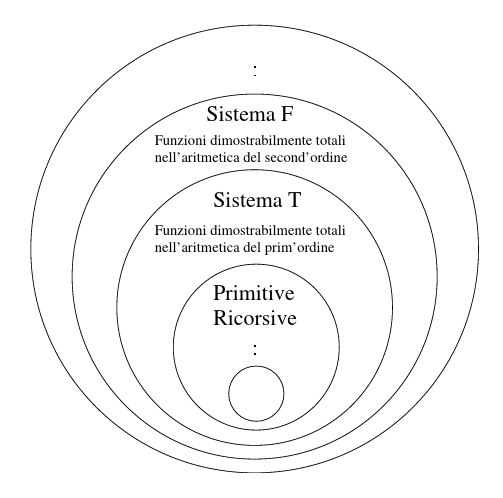
\includegraphics[scale=0.5]{img/TotalHierarchy.jpg}
    \caption{Gerarchia dei formalismi totali}
\end{figure}

\section{Tesi di Church}

Che succede se rinunciamo a questa idea della totalità? Sappiamo che non daremo luogo a paradossi.
Tuttavia rimane il problema: siamo nella situazione dei formalismi totali, e cioè esiste una
gerarchia di formalismi più potenti, o colpiamo un upper bound tale che in un formalismo del genere
posso calcolare tutte le funzioni che posso calcolare in qualsiasi altro formalismo?  Quest'ultima
situazione sembrerebbe miracolosa dati i risultati visti finora.

La cosa che era ragionevole aspettarsi era la prima. Quello che sembra essere, ma che non è
dimostrabile, è che la nozione di calcolabilità è indipendente dal formalismo che uso. Se ho un
formalismo abbastanza espressivo posso esprimere qualsiasi funzione intuitivamente calcolabile.
Questo è il succo della tesi di Church.

Quello che possiamo fare è confrontare formalismi a livello di potere espressivo. Più formalismi
si sono considerati più si è avvalorata l'idea che la classe di funzioni che possiamo calcolare sia
la stessa, ed in particolare quella delle funzioni calcolabili da una macchina di Turing.

La tesi di Church puo' essere espressa nella maniera seguente:
\begin{thm}
    Le funzioni calcolabili sono esattamente quelle intuitivamente calcolabili medi-
    ante una procedura effettiva di calcolo.
\end{thm}

Ci sono delle funzioni intuitivamente definibili ma non calcolabili? Non lo sappiamo. Rimane un
problema aperto.

\section{Alcuni formalismi Turing completi}

Dimostrare la Turing-completezza dei linguaggi moderni è complesso. Molti formalismi sono stati
studiati e sono stati trovati tutti equivalenti a potere espressivo.

Un sistema interessante è la logica combinatoria. Ho due costanti, che per ragione storiche si
chiamano $S$ e $K$. I programmi sono scritti come grosse combinazioni di $S$ e $K$. Ad esempio:
\begin{equation*}
    (K ((S K) K))
\end{equation*}

Abbiamo due regole di risctittura:
\begin{itemize}
    \item $((K M) N) \to M$ 
    \item $(((S P) Q) R) \to (P R) (Q R)$
\end{itemize}

È dimostrabile che questo sistema è Turing completo. Ovviamente c'è il problema di codificare i
dati di input e output. Questi sono quelli che sono chiamati combinatori.

Questi formalismi sono semplici. Si può dimostrare quindi l'equivalenza tra due formalismi come
meta-teorema in maniera agevole.

Il $\lambda$-calcolo è una di quelle cose dell'informatica che è così e non potrebbe essere
altrimenti. Si giustifica intrinsicamente. È la cosa più naturale, in un certo senso. La logica
combinatoria, ad esempio, non è così invece.

L'idea del $\lambda$-calcolo è che voglio un linguaggio per descrivere funzioni. Ho bisogno di:
\begin{itemize}
    \item variabili
    \item un meccanismo per definire funzioni. Introduciamo quindi, dato un termine $M$,$\lambda
    x. M$. Questa è l'operazione di introduzione (o costruzione) della funzione. Manca l'operazione di
    eliminazione (o distruzione)
    \item introduciamo quindi l'applicazione: $(M N)$
\end{itemize}
Posso partire da $x$ e, perché no, applicare $x$ a se stesso. Dopodiché introduco l'astrazione.
Ottengo $\lambda x. (x x)$.

Qual è la regola di calcolo? Questa nasce dall'interazione tra costruttore e distruttore.

Cosa mi aspetto da $(\lambda x. M) N$? Mi aspetto $M$ con tutte le occorrenze (libere) di x sostituite
da $N$:
\begin{equation*}
    (\lambda x. M) N \to M[N/x]
\end{equation*}

L'operatore visto prima è noto comunemente come $\delta = \lambda x. (x x)$. Definiamo $I$ come $I =
\lambda x. x$. È un formalismo di alto livello. Non ci sono tipi, posso applicare espressioni ad
altre espressioni senza limiti.

Consideriamo la seguente sequenza di calcolo dell'espressione $(\delta I)$:
\begin{equation*}
    (\delta I) \to (I I) \to I
\end{equation*}

$I$ è un termine in forma normale: non c'è più alcuna riduzione possibile per questo termine.

Cosa succede con $(\delta \delta)$? Si riscrive se stesso all'infinito.

Un altro formalismo è quello delle funzioni $\mu$-ricorsive.Cosa sono le funzioni $\mu$-ricorsive?
Si prende il formalismo primitivo ricorsivo e si aggiunge la minizzazione unbound. È Turing
completo.

Quando definiamo un formalismo abbiamo due modi. Un modo è quello descrittivo, ovvero definisco un
linguaggio ed eventualmente delle regole. È una descrizione ad alto livello. L'altro modo, un pò
più simile alle macchine di Turing o alle macchine a registri, è di dare un'architettura di basso
livello e scrivere i propri programmi utilizzando questa architettura.

\section{Macchine di Turing}

Finché lavoro con linguaggi ad alto livello è difficile convicersi che abbiano lo stesso potere
espressivo delle macchine di Turing. Inoltre rimane il dubbio: siamo sicuri di non aver tralasciato
un costrutto che permette di fare un balzo nel potere espressivo?

La macchina di Turing che consideriamo ha un nastro solo. È un nastro di memoria infinito. Esiste?
No, è un'astrazione matematica. E' diviso in celle di dimensione fissata. Ogni cella puo` contenere
un carattere di un alfabeto dato, compreso un carattere b (bianco) di inizializzaizone.

Abbiamo una testina di lettura mobile e un automa a stati finiti per la definizione del programma.

Un programma è composto da una lista infinita di operazioni che associano ad una coppia
$<\text{carattere},\text{stato interno}>$ una tripla $<$nuovo carattere, nuovo stato,
mossa$>$, dove mossa e' \textit{dx} o \textit{sx}.

Quello che possiamo fare è:
\begin{itemize}
    \item leggere e scrivere il carattere individuato dalla testina
    \item spostare la testina di una posizione verso destra o verso sinistra
    \item leggere e scrivere il carattere individuato dalla testina
\end{itemize}

Una Macchina di Turing (one-tape, deterministica) `e una tupla $<Q,\Gamma,b,\Sigma,\delta,q_{0},F>$
dove:
\begin{itemize}
    \item $Q$ `e un insieme finito di stati
    \item $\Gamma$ `e l'alfabeto finito del nastro
    \item $b$ `e il carattere bianco
    \item $\Sigma \subseteq \Gamma \setminus \set{b}$ `e l'insieme dei caratteri di input/output
    \item $q_{0} \in Q$ `e lo stato iniziale
    \item $F \subseteq Q$ `e l'insieme degli stati finali (o di accettazione)
    \item $\delta: Q \setminus F \times \Gamma \to Q \times \Gamma \times \set{L,R}$ `e la funzione di transizione.
\end{itemize}

La funzione di transizione ha un grafo finito. Ogni elemento del grafo `e una quintupla $(q, a, q',
a', M)$ tale che $(q, a) = (q', a', M)$. L'insieme finito delle quintuple può essere visto come
l'insieme delle istruzioni della macchina (programma), e la determina univocamente.

La computazione deve essere deterministica. Dato un input alla funzione di transizione ci può
essere un solo output.

Dobbiamo rispondere ad alcune considerazioni. Ad esempio, dove si trova la testina rispetto
all'input?  Innanzitutto suppuniamo che il nastro sia inizializzato con la stringa di input (un
carattere per ogni cella). Supponiamo poi che la testina parta dall'inizio dell'input. Tutte le
altre celle del nastro sono inizializzate col carattere speciale $b$.

Se abbiamo un nastro solo su quello scriviamo l'input e alla fine su quello troviamo l'output.
Dobbiamo decidere come interpretarlo; ci sono vari modi standard. Per noi nel momento in cui la
macchina si arresta l'output `e la piu` lunga stringa di caratteri in $\Gamma$ (in particolare,
senza $b$) alla destra della testina

Vediamo un esempio di macchina di Turing 

\begin{verbatim}
    -----------------
      |0|1|1|0|#|
    -----------------
       @
\end{verbatim}

Supponiamo di essere nello stato $q_{0}$ e di essere in posizione @. Consideriamo il seguente programma:
\begin{align*}
    <q_{0},0> &\to <q_{1},0,R>\\
    <q_{0},1> &\to <q_{2},1,R>\\
    <q_{1},0> &\to <q_{1},0,R>\\
    <q_{1},1> &\to <q_{1},1,R>\\
    <q_{1},\#> &\to <q_{3},0,R>\\
    <q_{3},1> &\to <q_{2},0,R>\\
    <q_{3},0> &\to <q_{4},\#,L>\\
    <q_{3},1> &\to <q_{4},\#,L>\\
    <q_{3},b> &\to <q_{4},\#,L>\\
    <q_{2},0> &\to <q_{2},0,R>\\
    <q_{2},1> &\to <q_{2},1,R>\\
    <q_{2},\#> &\to <q_{3},1,R>
\end{align*}

Possiamo associare $q_{1}$ allo stato ``ho letto uno zero''.

Questo programma copia il primo carattere in input nella posizione di \# e poi sposta \# a destra.

Abbiamo $Q = \{q_{0},\dotsc,q_{4}\}$ e $F = \{q_{4}\}$

Ad ogni coppia stato simbolo viene associata una tripla nuovo stato, nuovo simbolo e mossa. Ci sono
una infinità di varianti (tutte equivalenti dal punto di vista del potere formale).

La mossa da fare sarà unica perché la macchina è deterministica.

Una configurazione istantanea è una descrizione istantanea della configurazione della macchina. Non
corrisponde allo stato interno della macchina, ma quest'ultimo ne fa parte. La si può pensare come
ciò che devo ricordare per riprendere una computazione interrotta più tardi. Si parla di
configurazione solo in relazione ad un dato nastro di input.

Ho bisogno di salvare tre informazioni, avendo un nastro solo:
\begin{itemize}
    \item lo stato interno
    \item il nastro
    \item la posizione della testina sul nastro
\end{itemize}

L'ultimo passaggio è delicato: avrei bisogno di un'origine per definire la posizione. Non è però
chiaro definire dove sta questa origine. Avendo nastri infiniti non ho un'idea ben definita di
origine. Potrei fissarne una ma poi dovrei separare il nastro in due parti. Con un seminastro
sarebbe facile. La cosa più semplice è definire come origine il dove si trova la testina. A questo
punto mi interessa memorizzare solo il seminastro a destra della testina e quello a sinistra.

La mia configurazione sarà quindi:
\begin{equation*}
    \alpha,q,\beta
\end{equation*}

$\alpha$ è il seminastro sinistro, $\beta$ quello destro. Possiamo ora descrivere la comuputazione come
una sequenza di configurazioni.

Descriviamo la computazione di prima:
\begin{align*}
    &\emptyset,q_{0},0110\#\\
    &0,q_{1},110\#\\
    &01,q_{1},10\#\\
    &011,q_{1},0\#\\
    &0110,q_{1},\#\\
    &01100,q_{3},\emptyset\\
    &0110,q_{4},0\#
\end{align*}

Per comodità è sempre utile far vedere il primo carattere a destra e a sinistra della testina. Se
un seminastro è blank posso immaginare di avere $b$ come primo carattere:
\begin{equation*}
    \alpha,q,\beta \equiv \alpha_{1} a,q,b\beta_{1}
\end{equation*}

Supponiamo che questa sia la configurazione
\begin{equation*}
    \alpha a,q,b \beta
\end{equation*}
Supponiamo che questa sia l'istruzione
\begin{equation*}
    <q,b> \to <q',b',R>
\end{equation*}
Allora
\begin{equation*}
    <\alpha a,q,b \beta> \vdash <\alpha ab',q',\beta>
\end{equation*}

Analogamente, se $<q,b> \to <q',b',L>$ allora
\begin{equation*}
    <\alpha a,q,b \beta> \vdash <\alpha ,q',ab'\beta>
\end{equation*}

Questa è la semantica della macchina di Turing.

Il processore è a tutti gli effetti una macchina a stati finiti

Perché è importante l'idea della macchina di Turing? Perché la macchina di Turing racchiude il
concetto di operatore di calcolo più naturale che possiamo immaginare. 

Quello che l'agente esecutore ha a sua disposizione è una memoria illimitata. L'agente è un qualcosa
di finitistico, della memoria ha una visione finita. Quello che vede è la cella, di dimensione
finita ma senza alcuna assunzione sulla dimensione della cella. Non ha una visione sinottica
dell'intero nastro, ha una visione limitata dalla sua natura. L'agente può modificare una porzione
finita del nastro. Per semplicità diciamo che può modificare solo la cella.  Può spostarsi e
modificare il suo stato interno. Di quanto può spostarsi? Di una porzione finita. Può ripetere
queste azioni. Più di questo non può fare.

Perché è così potente questa nozione? Perché per andare oltre a questa nozione di calcolabilità
dovrei visionare e realizzare un agente di calcolo con capacità maggiori di quello descritto.

\section{Macchine universali}

Un'altra macchina interessante è la macchina universale. Questa è una macchina capace di eseguire
una qualsiasi macchina di Turing.

Perché ho bisogno di un nasto per memorizzare gli stati? Perché questi devono essere codificati, e
non so a priori quanto grande sarà la mia codifica.

\begin{verbatim}
    -------------------------------------------------------
        ||q_{0}|0|q_{1}|0|R||q_{1}|0|q_{1}|0|R||
    -------------------------------------------------------
    -------------------------------------------------------
        ||q_{0}|0||
    -------------------------------------------------------
    -------------------------------------------------------
        |0|1|1|0|#|
    -------------------------------------------------------
\end{verbatim}

Ho tre nastri: il nastro degli stati, il nastro che simula la macchina di Turing ed il nastro
dell'input. Ognuno ha la sua testina.

Perché è interessante questa macchina? Perché questa è, in sostanza, la macchina di Von Neumann,
eccetto per alcune differenze non significative. Ad esempio VN ha accesso random invece che un nastro
sequenziale.

Con le macchine di Turing ogni automa definiva un'architettura: servirebbero tante macchine quante
funzioni esprimibili. La macchina universale invece può emulare le macchine di Turing con un'unica
architettura. Ci sono differenze con la macchina di Turing ma sono dettagli, la struttura è simile e
le capacità della macchina universale non sono maggiori: il potere espressivo è lo stesso.
Prendiamo come input una macchina e l'input della funzione e la macchina universale fa da
interprete.

Noi passeremo ad una nozione ancora più astratta. Questo perché vogliamo una teoria della
calcolabilità che sia machine-independent. Non vogliamo essere costretti a ridurci sempre ad un
modello computazionale particolare.

L'idea è che dobbiamo pensare di avere una enumerazione dei programmi. $\phii$ è la funzione
calcolata dall'$i$-esimo programma. Noi diremo la funzione $i$-esima.

Vogliamo assicurarci che la numerazione dei programmi sia effettiva. Ad esempio, dato 100 voglio
sapere qual è il programma 100. Vogliamo quindi una funzione universale $\mu$ tale che:
\begin{equation*}
    \mu(i,x) = \phi_{i}(x)
\end{equation*}

Questa è la macchina universale o interprete. Possiamo vedere $i$ come la descrizione del programma.

Possiamo riformulare la tesi di Church in questo contesto come:
\begin{quote}
    ``$f \text{ è intuitivamente calcolabile } \implies \exists i. \phi_{i} = f$''
\end{quote}

%% tex/undecidableproblems.tex
%% Copyright 2019 Andrea Berlingieri
%
% This work may be distributed and/or modified under the
% conditions of the LaTeX Project Public License, either version 1.3
% of this license or (at your option) any later version.
% The latest version of this license is in
%   http://www.latex-project.org/lppl.txt
% and version 1.3 or later is part of all distributions of LaTeX
% version 2005/12/01 or later.
%
% This work has the LPPL maintenance status `maintained'.
%
% The Current Maintainer of this work is Andrea Berlingieri.
%
% This work consists of all files listed in manifest.txt
\chapter{Problemi indecidibili}

Ci chiediamo ora se ci sono dei problemi che non sono decidibili, ovvero non calcolabili in un
formalismo Turing completo. Introduciamo l'argomento con uno dei problemi più noti in letteratura,
l'\textit{Halting problem}.

Prima però chiariamo meglio i concetti di totalità, calcolabilità e la relazione tra i due, oltre
a introdurre i concetti di divergenza e convergenza.

\section{Note introduttive su programmi e funzioni}

Una qualsiasi funzione $\phii$ della nostra enumerazione delle funzioni calcolabili è una funzione
parziale calcolabile: su alcuni input può non essere definita. 

La calcolabilità non coincide con la totalità: esistono funzioni parziali calcolabili e funzioni
totali non calcolabili.

Le funzioni possono essere non definite in un punto. Se questo è il caso per una funzione
calcolabile $i$ ed un punto $x$, avremo allora la divergenza del \emph{programma} $i$: $\phii(x)
\diverges \iff \phii$ non è definita su input $x$. Divergenza e convergenza sono più proprietà del
programma che della funzione che calcola. Nonostante qui usiamo il simbolo $\phi$ sia per i
programmi che per le funzioni è bene ricordare che può avere un doppio ruolo e una semantica
diversa associata ad esso. La relazione tra i due è: la funzione $i$ nella mia enumerazione di
funzioni calcolabili è quella calcolata dal programma $i$ della mia enumerazione dei programmi.

La divergenza non è una proprietà generale delle funzioni. Non ha senso dire $\phii \diverges$ senza
specificare dove diverge; questo perché la convergenza e la divergenza sono proprietà puntuali:
valgono per un dato input. Al massimo $\phii(x)$ per un qualche $x$ può divergere.

\section{Il problema della fermata}

Il problema che ci interessa è il cosiddetto ``problema della terminazione''. Le funzioni che
stiamo calcolando sono funzioni parziali: i programmi corrispondenti possono potenzialmente
divergere. Noi vorremmo calcolare la seguente funzione:
\begin{equation*}
\textit{Term}(i,x) =
    \begin{cases}
        1 \quad & \text{se $\phii(x) \converges$} \\
        0 \quad & \text{se $\phii(x) \diverges$} 
    \end{cases}
\end{equation*}

Questà è la specifica della mia funzione. È una funzione totale. Ci chiediamo a questo punto, è
anche calcolabile? La risposta, come vedremo, sarà negativa.

Per dimostrarlo supponiamo che \textit{Term} sia calcolabile e prendiamo in considerazione ora la
funzione intermedia $g$:
\begin{equation*}
    g(x) =
    \begin{cases}
        1 \quad & \text{se $\textit{Term}(x,x) = 0$} \\
        \diverges \quad & \text{se $\textit{Term}(x,x) = 1$} 
    \end{cases}
\end{equation*}

Se \textit{Term} fosse calcolabile allora anche $g$ sarebbe calcolabile. Se $g$ è calcolabile deve
esistere un $k$ tale che $\phik = g$. Ci può essere più di un programma che calcola g, ma a me ne
basta uno.

Ci chiediamo ora, legittimamente, qual è il comportamento di $\phik(k)$? Converge?

Abbiamo che $\phik(k) = g(k)$. Quindi $\phik(k) \diverges \iff \textit{Term}(k,k) = 0 \iff g(k) = 1
\iff g(k) \converges \iff \phik(k) \converges$. Questo è contraddittorio. Verrebbe da concludere che
$\phik(k)$ converge. È tuttavia vero che $\phik(k) \converges \iff \textit{Term}(k,k) = 1 \iff g(k)
\diverges \iff \phik(k) \diverges$. Ma anche questo è contradditorio. L'ipotesi da cui siamo partiti
è che \textit{Term} fosse calcolabile. Concludiamo quindi che \textit{Term} non è calcolabile.

%T(i,x) = 
%\begin{cases}
%    1 se \phii(x) è definita \\
%    0 se \phii(x) è indefinita
%\end{cases}
%
%Useremo la notazione \phii(x) \converges e \phii(x) \diverges.
%
%Definiamo allora g(x):
%
%g(x) =  se T(x,x) = 0 restituisco 1
%        else \diverges
%
%Supponiamo che g sia \phi_{k}. Ci chiediamo: quanto vale T(k,k)? Ci sono due possibilità:
%
%0 = T(k,k) = g(k) = 1
%
%che è assurdo, oppure:
%
%1 = T(k,k) = g(k) = \diverges
%
%che è anche assurdo. Questo implica l'assurdità e la non calcolabilità di T.

È il primo caso di una funzione che possiamo pensare ma che non riusciamo a calcolare, almeno con questa
formulazione qui.

La dimostrazione è un semplice ragionamento diagonale. Esistono quindi funzioni ben definite ma non
calcolabili: non esiste un algoritmo che mi calcoli questo problema. Nella sua forma generale il
problema delle terminazione non è algoritmico.

Cosa vuol dire nella sua forma generale? Significa che valga per tutti gli $i$ e per tutti gli $x$.
Per alcuni programmi e alcuni input è possibile dimostrare che il programma termina. Ci sono dei
casi particolari che sono gestibili, ma non esiste un unico algoritmo che in modo uniforme su tutti
gli $i$ e tutti gli $x$ sappia decidere se il programma $i$ termini su input $x$.

Quali erano le nostre ipotesi? La calcolabilità dell'interprete e qualche piccola proprietà di
chiusura sul mio formalismo. Non molto.

Questa funzione non è esprimibile in un formalismo Turing completo. Non è tuttavia assurda l'idea
che esista un agente di calcolo con più capacità della macchina di Turing e che sia in grado di
calcolare \textit{Term}. È difficile da immaginare. Nella calcolabilità relativa si parte
immaginando un oracolo che sia capace di calcolare \textit{Term} e ci si chiede da lì cosa si possa
calcolare (e cosa no).

\section{Proprietà s-m-n}

%// TODO Va tenuta questa parte? C'entra poco.
%Nota: Quando ho statements del tipo \forall x \exists y, dove ho dipendenze funzionali tra y e x, se ho che
%ogni y è calcolabile in funzione di ogni x ho un teorema/dimostrazione intuizionistica/costruttiva.
%Altrimenti siamo nella matematica classica (dove vale il princio del terzo escluso e la RAA e dove
%nella mia dimostrazione non mostro gli x e y per cui vale). 

L'ipotesi della calcolabilità dell'interprete è un'ipotesi importante. Supponiamo, nella nostra
teoria della calcolabilità, che esista un modo per calcolarla. Questa proprietà è detta proprietà
UTM, Universal Turing Machine: $\exists u, \phiu(i,x) = \phii(x)$. È dimostrabile in tutti i
formalismi Turing completi.

La proprietà che andiamo ora a considerare è la cosiddetta proprietà s-m-n. Supponiamo di avere
una funzione calcolabile $g(x,y)$. Cosa posso dire delle sue istanze? Supponiamo di fissare $x$, ad
esempio a $0$. Ottengo $g(0,y)$, che è una funzione unaria che dipende solo da $y$. Possiamo indicare
$g(0,y)$ come $f_{0}(y)$. In generale posso fare questo per $f_{k}(y) = g(k,y)$.

Tutte queste funzioni sono calcolabili e quindi ognuna di esse farà parte della mia enumerazione
delle funzioni calcolabili. Esisterà quindi, per ognuna, un programma che la calcola. Esiste quindi
$\phi_{h(k)}(y) = f_{k}(y) = g(k,y)$ che mi calcola $g(k,y)$ per ogni $y$. $h$ è una funzione che
mi restituisce l'indice dell'istanza di $g$ che mi interessa. L'esistenza di $h$ è praticamente
ovvia: essendo tutte le istanze di $g$ relative a $k$ calcolabili avranno un indice nella mia
enumerazione delle funzioni calcolabili e questo indice dipende da $k$. La domanda ora è: $h$ è
calcolabile? La risposta è sì.

Noi supporremo la proprietà s-m-n, ma questa è facilmente dimostrabile in tanti formalismi.
\begin{thm}
    \textbf{Proprietà s-m-n. } $\forall g$ calcolabile $\exists h$ totale e calcolabile tale che
    \begin{equation*}
        \forall x,y. \phi_{h(x)}(y) = g(x,y)
    \end{equation*}
\end{thm}

Quello che stiamo facendo è una curryficazione. C'è un importante isomorfismo a livello di funzioni:
lo spazio delle funzioni $(A \times B) \to C$ è isomorfo allo spazio delle funzioni $A \to (B \to
C)$. L'operazione alla base della dimostrazione di questa affermazione e che mi permette di passare
da una funzione del primo spazio alla sua corrispondente nel secondo si chiama curryficazione.
L'idea è: data $g(x,y)$ fissiamo $x$. In questo modo ottengo $g(x,y)$, con $x$ fissato, ovvero una funzione
unaria in $y$ da $B$ a $C$.

Si può dimostrare anche con un argomento sulla cardinalità. Sappiamo che la cardinalità del primo
spazio è $|C|^{|A \times B|} = |C|^{|A|\cdot|B|} = (|C|^{|B|})^{|A|}$, che è la cardinalita di $A
\to B \to C$. Questo mi garantisce l'esistenza dell'isomorfismo. La dimostrazione precedente è un pò
più strutturale (e costruttiva se così si vuol dire).

$h$ fondamentalmente mi dà l'indice della funzione curryficata.

In un certo senso s-m-n mi dice che il mio formalismo è chiuso rispetto alle
curryficazioni/$\lambda$-astrazioni. UTM mi dice che il mio formalismo è chiuso rispetto alle
$\lambda$-applcazioni.

Possiamo generalizzare s-m-n a vettori $x$ e $y$ di parametri: 
\begin{thm}
    $\forall g \forall m \forall n \exists s$ totale calcolabile tale che
    \begin{equation*}
        \phi_{s(\vec{x}_{m})}(\vec{y}_{n}) = g(\vec{x}_{m},\vec{y}_{n})
    \end{equation*}
\end{thm}

s-m-n serve per calcolare un numero come indice di un programma. Se non bisogna calcolare un indice
di un programma in funzione di qualcos'altro non mi serve s-m-n. Noi vedremo molti casi in cui
avremo proprio bisogno di quello.

Vediamo un esempio di applicazione di s-m-n nella dimostrazione della non calcolabilità di alcune
funzioni.

La funzione che ci interessa indagare adesso è \textit{Tot} che determina se un certo programma è
totale o meno. È anche questo un problema di decisione. La specifica della mia funzione è:
\begin{equation*}
    \textit{Tot}(i) =
    \begin{cases}
        1 \quad &\text{se $\forall x \phii(x) \converges$} \\
        0 \quad &\text{altrimenti}
    \end{cases}
\end{equation*}

Abbiamo bisogno però prima di un risultato intermedio. Un caso particolare caso del problema della
terminazione è il problema della terminazione diagonale:
\begin{equation*}
    \textit{Term}(i) =
    \begin{cases}
        1 \quad &\text{se $\phii(i) \converges$} \\
        0 \quad &\text{se $\phii(i) \diverges$} \\
    \end{cases}
\end{equation*}

Se la terminazione diagonale non è calcolabile la terminazione generabile non è calolabile. Non è
vera l'implicazione inversa. Ha senso quindi chiedersi se la terminazione diagonale è calcolabile.
La risposta è no, e la dimostrazione è analoga a quella della terminazione generale.

Dimostrare che una funzione non sia calcolabile non è banale. Devo dimostrare che non esiste un
algoritmo tale che la calcoli. È molto più difficile rispetto a dimostrare la calcolabilità di una
funzione.

Abbiamo due strade. Assumiamo la calcolabilità di \textit{Tot} e troviamo un assurdo. Oppure usiamo
un procedimento di riduzione: se è calcolabile \textit{Tot} deve essere calcolabile
$\textit{Term}_{i}$. Da lì poi dimostriamo la non calcolabilità di $\textit{Term}_{i}$.

Prendiamo $g(i,x) = \phii(i)$. Abbiamo due casi: o converge o diverge. Nel primo caso se fisso $i$
la funzione curryficata che ottengo è totale. Nell'altro caso no.

Per s-m-n abbiamo $h$ totale e calcolabile tale che
\begin{equation*}
    \phi_{h(i)}(x) = g(i,x) = \phii(i)
\end{equation*}

Ora mi chiedo: quanto vale $\textit{Tot}(h(i))$? Abbiamo che
\begin{equation*}
    \textit{Tot}(h(i))=
    \begin{cases}
        1 \quad &\text{se $\phii(i) \converges$} \\
        0 \quad &\text{se $\phii(i) \diverges$}
    \end{cases}
\end{equation*}

Componendo \textit{Tot} con $h$ risolverei il problema della terminazione diagonale. Ma questo è
assurdo. Da cui \textit{Tot} non è calcolabile.

In questa dimostrazione parto da funzioni calcolabili che vado a comporre con la mia funzione di
partenza (\textit{Tot}) e ottengo una funzione che mi potrebbe calcolare qualcosa che so non essere
calcolabile. Da ciò concludo che la mia funzione di partenza non è calcolabile. È una
dimostrazione diversa da quella del problema della terminazione.

È interessante vedere questa dimostrazione anche ``al contrario'', in versione bottom up. Come
faccio a dimostrare la non calcolabilità di \textit{Tot}? Assumo che sia calcolabile e la uso per
risolvere un problema indecidibile. In questo caso vogliamo ridurci alla terminazione diagonale.
Come facciamo? Possiamo farlo cercando una funzione $h$ tale che, per ogni $i$, $\phi_{h(i)}$ è totale sse
$\phii(i) \converges$. Esiste questa funzione $h$? Sì, e possiamo dimostrarlo in due passaggi.

Per prima cosa definiamo una funzione calcolabile binaria $g(i,x)$ che, in base alla terminazione di
o meno di $\phii(i)$, ha un comportamento diverso che rispetti le condizioni che abbiamo posto su
$\phi_{h(i)}$. Ad esempio
\begin{equation*}
    g(i,x) =
    \begin{cases}
        1 \quad &\text{se $\phii(i)\converges$} \\
        \diverges \quad &\text{se $\phii(i)\diverges$} \\
    \end{cases}
\end{equation*}

Questa funzione è calcolabile? Sì, è facilmente scrivibile in un linguaggio di programmazione. Ma a
questo punto ho trovato la $h$ che cercavo, grazie alla proprietà s-m-n: $\exists h \text{ tot. e
calc.} \phi_{h(i)}(x) = g(i,x)$. A questo punto, se mi chiedo se la funzione $\phi_{h(i)}$ è totale,
utilizzando la funzione \textit{Tot}, mi sono ridotto al problema della terminazione diagonale.

Consideriamo un caso particolare e poi proviamo a generalizzare. Stiamo analizzando programmi. Mi
chiedo se un mio programma calcola la funzione identità. Si potrebbe generalizzare al capire se il
mio programma ha un certo comportamento rispetto ad una funzione di riferimento.

Vogliamo quindi
\begin{equation*}
    \textit{ID}(i) =
    \begin{cases}
        1 \quad &\text{se $\forall x, \phii(x) = x$} \\
        0 \quad &\text{altrimenti}
    \end{cases}
\end{equation*}

Possiamo dimostrare che questa funzione non è calcolabile, con la stessa tecnica di prima. Ci
riduciamo al problema della terminazione.

Costruiamo $g$ tale che
\begin{equation*}
    g(i,x) =
    \begin{cases}
        x \quad & \text{se $\phii(i) \converges$} \\
        \diverges \quad & \text{se $\phii(i) \diverges$}
    \end{cases}
\end{equation*}

Per s-m-n esiste $h$ tale che $\phi_{h(i)}(x) = g(i,x)$. Mi chiedo ora, $h(i)$ è la funzione
identita?

\begin{equation*}
    \textit{ID}(h(i)) =
    \begin{cases}
        1 \quad &\text{se $\phii(i) \converges$} \\ 
        0 \quad &\text{ se $\phii(i) \diverges$} \\
    \end{cases}
\end{equation*}

Bisogna partire da una funzione calcolabile, altrimenti non si può applicare s-m-n. È parte
fondamentale della dimostrazione mostrare che $g$ è calcolabile.

\section{Il predicato $T$ di Kleene}

Ci chiediamo ora se esista un predicato calcolabile $T(i,x,t)$ che mi dice se il programma $i$
termina la computazione su input $x$ entro il tempo $t$.

C'è il problema di come definiamo il tempo; tuttavia l'idea è che tutti i programmi di cui
parliamo sono di tipo discreto, hanno un passo discreto di calcolo.

È calcolabile? Intuitivamente sì. Immaginiamo di avere un interprete. Interpretiamo il programma
$i$, seguendolo passo per passo per input $x$. Se dopo $t$ passi la computazione è terminata allora
ho una risposta positiva; in caso contrario no.

Esistono tante varianti del predicato $T$ di Kleene. Questa è una forma ``ternaria''. Possiamo pensare
ad una versione ``quaternaria'' $T^{4}(i,x,y,t)$ che mi dice se il mio programma termina su output
$y$ in $t$ o meno passi su input $x$.

La forma originale di Kleene era un predicato ternario $T(i,x,\textit{tr})$, dove \textit{tr} è una
traccia computazionale. Si può vedere come una sequenza di configurazioni istantanee. Non deve
essere necessariamente completa, deve essere corretta. È ancora chiaramente decidibile se la traccia
seguita sia quella passata in input. Questa forma in un certo senso comprende le prime due. L'idea è
che la lunghezza della traccia è il tempo passato dall'inizio della computazione.

Si può addirittura dimostrare che $T$ è primitivo ricorsivo in generale. Inoltre ha una complessità
computazionale relativamente bassa. La complessità è lineare in $t$ e nelle altre componenti.

C'è un corollario del predicato $T$ di Kleene. Se supponiamo questo predicato come primitivo
possiamo scrivere, sulla base di questo, la macchina universale, la cui esistenza smette di essere
primitiva nella nostra teoria della calcolabilità.

Infatti possiamo definire $u$ nel seguente modo:

\begin{equation*}
    u(i,x) = \textit{fst}(\mu <y,t>, T(i,x,y,t))
\end{equation*}

Questo corrisponde a scrivere $\textit{fst}(\mu w, T(i,x,\textit{fst}(w),\textit{snd}(w)))$. Il
\textit{fst} più esterno serve perché a me non interessa $t$, interessa $y$.

Questo è un risultato importante e si chiama forma normale di Kleene. C'è un corollario
importante. Si potrebbe limitare sintatticamente un programma ad un while con all'interno un for e
questo non diminuirebbe il potere espressivo del formalismo, poichè l'interprete è scrivibile in
questi termini.

Un altro problema non calcolabile è il problema del raggiungimento di codice. Ovvero, dato un
programma e un'istruzione il problema di decidere se il programma raggiungerà mai quell'istruzione
non è calcolabile. Esistono delle tecniche ma queste non sono generali. Sono tipicamente usate dai
compilatori per ottimizzare il codice oggetto ed eliminare parti di codice inutile.

%% tex/recursivesets.tex
%% Copyright 2019 Andrea Berlingieri
%
% This work may be distributed and/or modified under the
% conditions of the LaTeX Project Public License, either version 1.3
% of this license or (at your option) any later version.
% The latest version of this license is in
%   http://www.latex-project.org/lppl.txt
% and version 1.3 or later is part of all distributions of LaTeX
% version 2005/12/01 or later.
%
% This work has the LPPL maintenance status `maintained'.
%
% The Current Maintainer of this work is Andrea Berlingieri.
%
% This work consists of all files listed in manifest.txt
\chapter{Insiemi ricorsivi e ricorsivamente enumerabili}

Supponiamo di voler trasmettere un insieme. Se questo è finito non c'è nessun problema, basta
mandare i suoi elementi. Se ho un insieme infinito posso trasmettere il programma che calcola la
funzione caratteristica del mio insieme. Non posso immaginare di poter trasmettere tutti gli insiemi
in questo modo, altrimenti potrei risolvere il problema della terminazione diagonale. Quelli per
cui è possibile sono detti ricorsivi.

% definition?
\begin{defn}
    Un insieme $A$ è ricorsivo sse $c_{A}$ è calcolabile.
\end{defn}

Un altro modo per trasmettere il mio insieme in maniera effettiva è dare un metodo di calcolo,
detto funzione enumerativa. Supponiamo di avere un insieme ${a_{0},a_{1},a_{2},\dotsc}.$ Diamo una
funzione $f$ tale che $f(0) = a_{0}$, $f(1) = a_{1}$, ecc. Abbiamo che $A = \cod(f)$.

Quando posso dare l'insieme in questa maniera ed $f$ è calcolabile si dice che l'insieme è
ricorsivamente enumerabile. Ricorsivamente è terminologia veccha, degli anni trenta del XX secolo.
In queste due accezioni ricorsivo va visto come sinonimo di calcolabile.

\begin{defn}
    $A$ è ricorsivamente enumerabile sse esiste una funzione di enumerazione $f$ per $A$
    calcolabile: $A = \cod(f)$, per $f$ calcolabile.
\end{defn}

\section{Relazione tra insiemi ricorsivi e r.e.}

Esistono quindi sostanzialmente due modi per descrivere in maniera effettiva un insieme $A$.
Vogliamo capire che relazione c'è tra queste due nozioni: qual è più potente? Come si rapportano?

Per descrivere una classe è spesso utile capire rispetto a quali operazioni la classe è chiusa. In
particolare, se $A$ è ricorsivo cosa possiamo dire del complementare di $A$, o
dell'unione/intersezione/differenza di $A$ con un altro insieme ricorsivo?

Ricordiamo che $A \subseteq \Nat$. Abbiamo che:
\begin{itemize}
    \item $\emptyset$ è ricorsivo: la funzione costante $\bm{0}$ è calcolabile;
    \item $\Nat$ è ricorsivo: la funzione costante $\bm{1}$ è calcolabile;
    \item ogni insieme finito è ricorsivo: $D$ è finito $\implies$ $D$ è ricorsivo:
    \begin{equation*}
        c_{D}(x) = 
        \begin{cases}
            1 \quad & \text{se $x = d_{1} \lor x = d_{2} \lor \dotsc \lor x = d_{n}$}  \\
            0 \quad & \text{altrimenti}
        \end{cases}
    \end{equation*}
    Sarebbe esprimibile anche con una serie di \textit{if}. Qualunque sia $D$ ho un modo per scrivere la mia
    funzione caratteristica.
\end{itemize}

Con lo stesso ragionamento posso dimostrare che molte altre funzioni sono calcolabili. Ad esempio
una funzione con \textit{Range} finito è sicuramente calcolabile; è scrivibile con un \textit{case}
ad esempio.  Tutte le funzioni scrivibili con un \textit{case} sono sicuramente calcolabili. Queste
funzioni hanno sempre un numero finito di elementi su cui hanno un comportamento interessante e nei
restanti hanno lo stesso comportamento.

L'insieme dei numeri pari è ricorsivo. Tutti gli insiemi primitivi ricorsivi, ovvero con funzione
caratteristica primitiva ricorsiva, sono sicuramente ricorsivi. Infatti le funzioni primitive
ricorsive sono un caso particolare di algoritmo.

Esistono insiemi non ricorsivi. Ad esempio $K = \{i \mid \phii(i) \converges\}$ non è ricorsivo.

Supponiamo che $A$,$B$ siano ricorsivi. Abbiamo che:
\begin{itemize}
    \item $\comp{A}$ è ricorsivo. Questo perche $c_{\comp{A}}(x) = 1 - c_{A}(x)$
    \item $A \cup B$ è ricorsivo. Questo perche $c_{A \cup B}(x) = \max(c_{A}(x),c_{B}(x))$
    \item $A \cap B$ è ricorsivo. Questo perche $c_{A \cap B}(x) = \min(c_{A}(x),c_{B}(x))$
\end{itemize}

Gli insiemi ricorsivi formano un'algebra di Boole, essendo chiusi per queste tre operazioni. Sono
una sottostruttura interessante degli insiemi.

Data una funzione caratteristica è facile costruire una funzione di enumerazione. In altri termini,
se un insieme è ricorsivo è anche ricorsivamente enumerabile. C'è un piccolo inghippo però a cui
bisogna fare attenzione.

La funzione di enumerazione potrebbe essere costruita nel seguente modo ad esempio:
% python snippet
\begin{python}
    def $e_{A}(i)$:
        $c$ = 0
        $j$ = 0
        while $c \leq i$:
            if $c_{A}(j)$:
                $c++$
            $j++$
        return $j-1$
\end{python}

In versione funzionale potremmo scrivere scrivere $e_{A}$ come $e_{A}(i+1) = \mu j, c_{A}(j) = 1
\land j > e_{A}(i)$, con $e_{A}(0) = \mu j, c_{A}(j) = 1$. Il piccolo dettaglio a cui fare
attenzione è che la funzione di enumerazione la vorremmo totale e calcolabile. Tuttavia questo non è
un vincolo così restringente.

Diamo la seguente definizione: $A$ è r.e. se esiste $f$ totale calcolabile tale che $A = \cod(f)$
oppure $A$ è vuoto.

Il problema della nostra funzione di enumerazione è che può divergere con insiemi finiti. Se, ad
esempio, ho un $A$ con 7 elementi e cerco l'ottavo con la mia funzione avrò che divergerà.

Il teorema rimane, se $A$ è ricorsivo è ricorsivamente enumerabile. Bisogna giusto ricordarsi che
per gli insiemi finiti va fatto un caso speciale che gestisca input maggiori della cardinalità di
$A$.

Più precisamente, se $A$ è finito, con $A = {a_{0},\dotsc,a_{n}}$, allora definiamo $e_{A}$ nel
seguente modo:
\begin{equation*}
    e_{A}(x) = 
        \begin{cases}
                x = 0 \Rightarrow a_{0} \\
                x = 1 \Rightarrow a_{1} \\
                \vdots \\
                x = n \Rightarrow a_{n} \\
                \textit{default} \Rightarrow a_{n}
        \end{cases}
\end{equation*}

%Abbiamo che $A$ è ordinato rispetto all'ordinamento sui naturali. Di conseguenza le mie due funzioni
%sono monotone crescenti (seguiamo l'ordine) e possiamo ordinare l'insieme in maniera almeno non
%decrescente (strettamente crescente nel caso di insiemi finiti).

Abbiamo quindi che Ricorsivo $\implies$ R.E. Vale il viceversa? La risposta è no, ma non è del tutto
ovvia.

Sia $A$ un insieme r.e. Potremmo pensare di calcolare la funzione caratteristica di $A$ con la sua
funzione di enumerazione, nel seguente modo:
\begin{python}
    def $c_{A}(x)$:
        $i$ = 0
        while $e_{A}(i) \not= x$:
            $i++$ 
        return 1
\end{python}

Questa $c_{A}$ però non calcola la funzione caratteristica di $A$, bensì la funzione
semicaratteristica di A,che indicheremo con $s_{A}$.
\begin{equation*}
    s_{A}(x) =
    \begin{cases}
        \case{1}{se $x \in A$} \\
        \case{\diverges}{altrimenti}
    \end{cases}
\end{equation*}

Questa funzione è calcolabile e parziale. Per ora abbiamo dimostrato che la funzione
semicaratteristica di $A$ è calcolabile, non abbiamo ancora dimostrato che r.e. $\centernot\implies$
ricorsivo. Dobbiamo mostrare un esempio di insieme r.e. che non sia ricorsivo. $K$ è non
ricorsivo. $K$ è r.e.?

Proviamo a scrivere una funzione di enumerazione per $K$:
\begin{python}
    def $e_{K}(\pair{i}{t})$:
        if $T^{3}(i,i,t) = 1$:
            return i
        else:
            return $k_{0}$
\end{python}
        
Nell'else è importante che restituisca un programma che sta in $K$. Ce ne sono tanti e di semplici;
ad esempio le funzioni costanti. Diamo indice $k_{0}$ ad un tale programma.

È una buona funzione di numerazione? È sicuramente calcolabile. È suriettiva? È facile vedere che
numero solo cose che stanno in $K$: $k_{0}$ sta in $K$ e se restituisco $i$ allora $i$ stava in $K$.
Se $i$ sta in $K$ vuol dire che esiste un $t$ tale che $\phii \converges$ in $t$ passi. Di conseguenza
vengono enumerate tutte le funzioni convergenti su $i$ di indice $i$. 

Il dovetailing è al variare dell'input. Mi muovo sugli input e sul tempo di computazione.

Si potrebbe fare anche nel seguente modo:
\begin{equation*}
    e_{K}(c) = fst(\mu \pair{i}{t}, \pair{i}{t} \geq c \land T(i,i,t))
\end{equation*}

Il risultato finale è che $K$ è ricorsivamente enumerabile.

C'è un'altra relazione notevole tra insiemi r.e. e insiemi ricorsivi.

\begin{thm}
    Sia $A$ un insieme tale che sia $A$ che $\comp{A}$ sono r.e. Allora $A$ è ricorsivo.
\end{thm}
\begin{proof}
    Supponiamo di aver $e_{A}$ ed $e_{\comp{A}}$. Informalmente, possiamo far partire la ricerca per
    entrambe le funzioni. Prima o poi una terminerà, e in base a quale termina ho la mia risposta. La
    computazione parallela è assolutamente algoritmica e non c'è problema al riguardo.

    Più formalmente, sia $h$ così definita:
    \begin{equation*}
        h(x) =
        \begin{cases}
            \case{e_{A}(x)}{se $x = 2n$ per qualche $n$} \\
            \case{e_{\comp{A}}(x)}{se $x = 2n+1$ per qualche $n$} \\
        \end{cases}
    \end{equation*}
    Possiamo scrivere $c_{A}(n) = \textit{pari}(\mu i, h(i) = n)$
\end{proof}

Come corollario di questo teorema abbiamo che esiste un insieme nè ricorsivo nè r.e. Quale?
$\comp{K}$. Se infatti $\comp{K}$ fosse r.e. allora $K$ sarebbe ricorsivo.

Abbiamo una gerarchia degli insiemi fatta in questo modo: 

\begin{figure}[h]
    \centering
    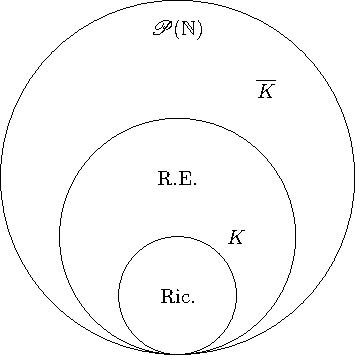
\includegraphics{./img/recursivesets/RecursiveHierarchy.pdf}
    \caption{Gerarchia degli insiemi r.e. e ricorsivi}
\end{figure}

\newpage

\section{Enumerazioni iniettive e monotone}

Ci concentriamo ora sulle proprietà dell'enumerazione. Ci chiediamo in particolare cosa possiamo
dire riguardo alla sua monotonia e alla sua iniettività.

Supponiamo di poter enumerare $A$ con una funzione effettiva. Ci chiediamo se possiamo trasformare
$f$ in modo da non avere ripetizioni. Se pensiamo all'enumerazione come ad uno stream infinito di
numeri in input ci chiediamo se possiamo creare un filtro che elimini i duplicati dallo stream.

Questo si può fare in maniera algoritmica tenendo una lista dei numeri ricevuti dallo stream e, ogni
volta che ho un nuovo numero, controllo se è gia nella lista. In base al risultato decido se
aggiungerlo o meno alla lista. La mia lista è ora il mio nuovo stream senza ripetizioni. Abbiamo
quindi che non è restittivo richiedere che la mia enumrazione sia iniettiva.

Diamo quindi la seguente definizione:

\begin{defn}
    $A$ è R.E. sse $\exists f$ iniettiva tot. calc. tale che $A = \cod(f)$ oppure $A$ è finito.
\end{defn}

A livello formale data l'enumerazione $f$ possiamo costruire una nuova enumerazione $g$ per lo
stesso insieme che sia iniettiva nel seguente modo:
\begin{equation*}
    g(x) =
    \begin{cases}
        \case{f(0)}{se $x = 0$} \\
        \case{f(\mu i, \forall y \leq x-1, f(i) \not= g(y))}{altrimenti}
    \end{cases}
\end{equation*}

Questo ha senso per insiemi infiniti.

L'iniettività è quindi una proprietà accettabile per la mia enumerazione. Posso trasformarla anche
in una funzione monotona crescente? La risposta sarà no, non posso enumerare gli elementi di $A$ in
maniera crescente se $A$ è r.e.

Il problema è fondamentalmente che non posso assicurarmi che un dato elemento sia il più piccolo
nello stream. La ricerca divergerebbe. Ogni volta che cerchiamo un minimo c'è un problema del
genere.

L'idea è che se potessimo ordinare gli elementi di $A$ allora $A$ sarebbe ricorsivo. Dato che non tutti
gli insiemi r.e. sono ricorsivi non si può fare in generale.

Sia $f$ un'enumerazione strettamente crescente. Essendo discreta cresce strettamente più
dell'identità. Se voglio sapere se $x$ fa parte della mia numerazione posso controllare gli elementi
fino ad $x$, oltre sicuramente non lo troverò.

Più formalmente, la ricerca di $x$ può essere fatta col seguente algoritmo:
\begin{python}
    $i_{x}$ = $\mu i, f(i) \geq x$
    return ($f(i_{x}) == x$)
\end{python}

In questo modo sono sicuro, se $f$ è strettamente crescente, che la mia ricerca termina. Per capire
se $x$ stava nel mio stream controllo che $f(i_{x})$ sia uguale ad $x$. 

Questo algoritmo funziona se la mia funzione è non decrescente? Se la mia funzione diventa
indefinitamente costante da un certo punto in poi potrei andare avanti all'infinito. La mia
minimizzazione non ha più garanzia di terminare.

Questo problema sorge quando $\cod(f)$ è finito. Quando $\cod(f)$ è infinito prima o poi la funzione
assumerà un nuovo valore. Tuttavia se $\cod(f)$ è finito allora l'insieme enumerato da $f$ è
ricorsivo.

Ogni insieme ricorsivo infinito è enumerabile mediante una funzione di enumerazione crescente. Ogni
insieme ricorsivo non vuoto è enumerabile mediante una funzione di enumerazione non decrescente.

Se si è in grado di ordinare si è anche in grado di decidere. Gli approcci generativi sono
generalmente semidecidibili e permettono di generare elementi in maniera disordinata.

Riprendiamo ora $K = \{i \mid \phii(i) \converges\}$. Come decidiamo se un certo $i$ sta in $K$? Possiamo far
partire il mio interprete e aspettare. Se termina allora $i$ appartiene a $K.$ Se non appartiene a
$K$ non lo saprò mai, perché dovrei aspettare che il programma termini. Di $K$ non possiamo quindi calcolare
la funzione caratteristica, bensì la funzione semicaratteristica:
\begin{equation*}
    s_{K}(i) = 
    \begin{cases}
        \case{1}{se $\phii(i) \converges$} \\
        \case{\diverges}{altrimenti}
    \end{cases}
\end{equation*}

In generale la funzione semicaratteristica di $A$, con $A$ r.e., è fatta nel seguente modo:
\begin{equation*}
    s_{A}(x) = 
    \begin{cases}
        \case{\converges}{se $x \in A$} \\
        \case{\diverges}{se $x \notin A$}
    \end{cases}
\end{equation*}

In alcuni casi posso semidecidere la appartenenza di un elemento ad un insieme, in altri casi potrei
non esserne in grado.

\section{Insiemi r.e. e semidecisione}

Ci chiediamo ora che legame esista tra la capacità di enumerare e la capacità di semidecidere. Ce
lo chiediamo in generale, ricordando che per $K$ l'abbiamo già visto.

Supponiamo che $A$ sia vuoto oppure $A = \cod(f)$, con $f$ tot. calcolabile. Come faccio a costruire
l'algoritmo di semidecisione per $A$? Semplicemente comincio a cercare $x$ nell'enumerazione.
\begin{equation*}
    s_{A}(x) = (\mu i, (f(i) = x))
\end{equation*}

Come facciamo per il viceversa? Abbiamo la procedura di semidecisione per $A$ e vogliamo costruire la
funzione di enumerazione per $A$. $f$ è delicata perché potrebbe divergere. Dobbiamo essere più
astuti. L'idea è muoversi mediante dove tailing sull'input e sul tempo di computazione.
\begin{equation*}
    f(\pair{x}{t}) =
    \begin{cases}
        \case{x}{se $s_{A}(x)$ termina nel tempo $t$} \\
        \case{a_{0}}{altrimenti}
    \end{cases}
\end{equation*}

$f$ è totale e calcolabile. Abbiamo quindi un'enumerazione per $A$. Non è iniettiva, ma questo non
importa. $a_{0}$ è un elemento qualsiasi di $A$. Possiamo quindi vedere la semidecisione come
enumerazione di un insieme r.e. e viceversa.

Non siamo sicuri di poter trovare $a_{0}$. Questo pezzo della dimostrazione è non costruttivo. Dal
punto di vista classico però o l'insieme è vuoto, e quindi r.e., oppure non lo è e deve avere almeno
un elemento $a_{0}$. Deve quindi esistere la funzione calcolabile $f$, anche se non è detto che
possiamo trovarla.

Vediamo ora un'applicazione. Quali sono le proprietà di chiusura per gli insiemi r.e.? Sono chiusi
per complementazione? No, altrimenti gli insiemi r.e. sarebbero tutti ricorsivi, e sappiamo che
questo non è vero. Ad esempio $K$ è r.e. e $\comp{K}$ non lo è.

Cosa possiamo dire di $A \cup B$ e $A \cap B$? Per $A \cup B$ è abbastanza ovvio. Dati $f_{A}$ e
$f_{B}$ possiamo costruire $f_{A \cup B}$ in modo che $f_{A \cup B}(2x) = f_{A}(x)$ e $f_{A \cup
B}(2x + 1) = f_{B}(x)$. Per $A \cap B$ è semplice costruire il semidecisore di $A \cap B$ dati
quelli per $A$ e per $B$. Basta concatenare i due: $s_{A \cap B}(x) = s_{A}(x);s_{B}(x)$.

Piccola nota sulla notazione. Noi consideriamo funzioni parziali da $\Nat$ a $\Nat$: $f: \Nat
\partialto \Nat$. Indichiamo, in maniera impropria, $\cod(f) = \{y \mid \exists x, y = f(x)\}$ e
$\dom(f) = \{x \mid f(x) \converges\}$. Il nostro codominio in realtà è il \textit{Range} della
funzione ed il nostro dominio è il dominio di congergenza (o co-\textit{Range}). In termini del grafo abbiamo che $\dom(f)
= \{x \mid \exists y, \pair{x}{y} \in \textit{grafo}(f)\}$.

\section{Caratterizzazioni alternative di un insieme r.e.}

Vediamo ora alcune caratterizzazioni, tutte equivalenti, degli insiemi r.e. che sono più adatte in
certi contesti.

Se si può caratterizzare un insieme r.e. $A$ come il dominio di convergenza di una funzione $s$ abbiamo
che $s$ rappresenta la funzione di semidecisione di $A$.

Abbiamo visto che $A$ è r.e. sse $A = \emptyset \lor A = \cod(f)$, $f$ tot. calc.

Abbiamo però che $A$ può essere visto come $\dom(g)$, con $g$ parz. calc. È una definizione
equivalente a quella appena citata.

Si può infine definire $A$ anche come $A = \cod(h)$, con $h$ parz. calc.

Solitamente quando costruiamo una funzione di enumerazione la vogliamo totale, è meno problematica.

Le tre definizioni sono equivalenti appena viste sono equivalenti. 

\begin{thm}
    Le tre seguenti affermazioni sono equivalenti e definiscono tutte un insieme r.e. $A$:
    \begin{enumerate}
        \item \label{re1} $A = \emptyset \lor A = \cod(f)$, con $f$ totale calcolabile \\
        \item \label{re2} $A = \dom(g)$, con $g$ parziale calcolabile \\
        \item \label{re3} $A = \cod(h)$, con $h$  parziale calcolabile
    \end{enumerate}
\end{thm}
\begin{proof}
    Lo dimostriamo facendo vedere che $\eqref{re1} \implies \eqref{re2}$, $\eqref{re2} \implies
    \eqref{re3}$ e $\eqref{re3} \implies \eqref{re1}$.

    \begin{itemize}
        \item $\eqref{re1} \implies \eqref{re2}$:

        Se $A = \emptyset$, allora abbiamo che $A = \dom(f_{\emptyset})$, se indichiamo con
        $f_{\emptyset}$ la funzione ovunque divergente.

        Se invece $A \not= \emptyset$ sia $f$ tale che $A = \cod(f)$. Definiamo $g$ come
        \begin{equation*}
            g(x) = \mu y, f(y) = x
        \end{equation*}
        
        Si ha che $A = \dom(g)$.

        \item $\eqref{re2} \implies \eqref{re3}$:

        Sia $A = \dom(g)$, con $g$ parziale calcolabile. Sia $h$ la funzione calcolata dal seguente
        programma:
        \begin{python}
            def $h(x)$:
                $g(x)$ 
                return $x$ 
        \end{python}
        Se $g(x)$ termina restituisco $x$. Si ha che $A = \cod(h)$.

        \item $\eqref{re3} \implies \eqref{re1}$: 
        
        Abbiamo due casi: $A$ è vuoto oppure no.

        Se $A = \emptyset$ l'asserto è già dimostrato.

        Se $A \not= \emptyset$ allora $\exists a \in A$. A questo punto definisco la mia $f$ come:
        \begin{equation*}
            f(\pair{x}{t}) = 
            \begin{cases}
                \case{h(x)}{se $h(x)$ termina entro il tempo $t$}\\
                \case{a}{altrimenti}
            \end{cases}
        \end{equation*}

        $f$ è totale, perché do sempre in output un valore. È calcolabile, sotto l'ipotesi che $h$
        sia calcolabile. Infine $\cod(f) = A$ perché $f$ restituisce solo elementi in $A$ e me li
        restituisce tutti, dato che $A = \cod(h)$.
    \end{itemize}
\end{proof}


La definizione \eqref{re3} ci permette di non doverci soffermare sul caso particolare dell'insieme
vuoto, che non ha implicazioni tecniche importanti.

\subsection{Teorema della proiezione}

Un'ulteriore caratterizzazione degli insiemi r.e. è la seguente:

\begin{thm}
    $A$ è r.e. sse $\exists B$ ricorsivo tale che $A = \{x \mid \exists y, \pair{x}{y} \in B\}$.
\end{thm}
\begin{proof}
    Vediamo i due versi del $\iff$ separatamente:
    \begin{itemize}
        \item $\implies$ Sia $c_{B}$ la funzione caratteristica di $B$. Allora $A = \dom(f)$, con
        \begin{equation*}
            f(m) = \mu n, c_{B}(\pair{n}{m}) = 1
        \end{equation*}
        \item $\implied$ Sia $A = \dom(\phii)$. Quindi $m \in A$ sse $\phii(m) \converges$, ovvero
        se $\exists t, T^{3}(i,m,t) = 1$, dove $T$ è il predicato ternario di Kleene.
        Basta quindi porre:
        \begin{equation*}
            B = \set{\pair{m}{t} \mid \exists t, T^{3}(i,m,t)}
        \end{equation*}
    \end{itemize}
\end{proof}

Possiamo vedere $B$ come una codifica delle coppie oppure come un insieme di coppie, non è
importante.

$A$ è la proiezione esistenziale di $B$ 

\begin{figure}[h]
    \centering
    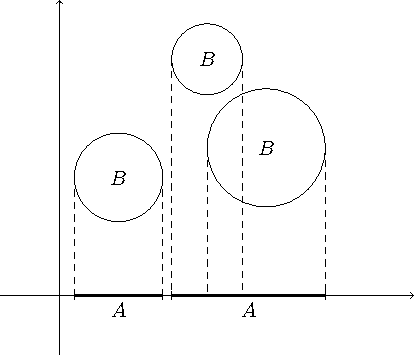
\includegraphics{./img/recursivesets/ExistentialProjection.pdf}
    \caption{Proiezione esitenziale di $B$}
\end{figure}

Il teorema è importante. Se ho un insieme ricorsivo e ne faccio la proiezione esistenziale ottengo
un insieme r.e. $x \in A$ sse $\exists y, (x,y) \in B$. Posso verificare se $(x,y)$ sta in $B$
perché $B$ è ricorsivo. Posso quindi semidecidere l'appartenenza di $x$ ad $A$ con un algoritmo del
genere ad esempio: $\mu y, (x,y) \in B$.

Se io faccio una ricerca in un dominio ricorsivo non è detto che questa termini. Se potessi dare dei
bound alla mia ricerca o avessi altre ipotesi potrei trasformare il mio algoritmo di semidecisione
in un algoritmo di decisione, ma in generale non è questo il caso. Avremo in generale una funzione
di semidecisione.

L'altra conseguenza importante è che qualunque problema semidecidibile può essere visto come una
ricerca in uno spazio decidibile.

È utile vedere $y$ come certificato di $x$, $c_{x}$. Il fatto che $x$ appartenga ad $A$ è cerficato da
$c_{x}$. Se $x \in A$ sappiamo che questo ceritificato esiste ma non sappiamo quale sia. La sua
ricerca non è però un problema decidibile.

Prendiamo per esempio la logica del prim'ordine. Se ho una formula in generale non è decidibile se
questa sia dimostrabile. Tuttavia abbiamo un algoritmo che genera tutte le formule dimostrabili nella
logica del prim'ordine. Dimostrare $F$ con questo algoritmo significa andare a cercare, nell'insieme
delle formule generate, un certificato per $F$. 

Un altro esempio è: dato un programma datemi un certificato per la sua appartenenza a $K$. Questo
certificato potrebbe essere il tempo $t$ in cui $\phi_{x}(x)$ termina. La dimostrazione che abbiamo
visto procede proprio in questo modo.

Il certificato non è un concetto ben definito, sta a noi decidere cosa sia un certificato. Un
certificato per un teorema potrebbe benissimo essere sia una prova che semplicemente la dimensione
della prova.

Ritorneremo su questo concetto quando parleremo di $\PClass$ e $\NPClass$. Vedremo che $\NPClass$ è l'insieme dei
linguaggi che sono proiezione esistenziale di un qualche linguaggio in $\PClass$. 

La caratterizzazione $A = \dom(\phii)$ è così importante che abbiamo della notazione specifica per
indicarlo: $W_{i}$. Possiamo con questa notazione definire $K$ come $K = \{i \mid i \in W_{i}\}$.
L'importanza di questa caratterizzazione è data dal fatto che essa induce una enumerazione di tutti
gli insieri r.e., basata sui domini di convergenza delle funzioni della mia enumerazione delle
funzioni calcolabili.

\section{Ulteriori proprietà di chiusura degli insiemi r.e.}

\begin{thm}
    Siano $A,B \subseteq \Nat$ e $f : \Nat \to \Nat$. Abbiamo che:
    \begin{enumerate}
        \item se $A$ è ricorsivo e $f$ è totale calcolabile, allora $f^{-1}(A)$ è ricorsivo
        \item se $A$ è r.e. e $f$ è calcolabile, allora $f^{-1}(A)$ è r.e.
        \item se $A$ è r.e. e $f$ è calcolabile, allora $f(A)$ è r.e.
    \end{enumerate}
\end{thm}
\begin{proof}
    Vediamo i tre punti uno per uno:
    \begin{enumerate}
        \item $c_{f^{-1}(A)}(x) = c_{A}(f(x))$
        \item Sia $A = \dom(g)$, con $g$ calcolabile. Consideriamo la seguente funzione:
        \begin{equation*}
            h(x) = g(f(x))
        \end{equation*}
        Questa funzione termina su $x$ sse $x \in \dom(f) \land f(x) \in \dom(g)$. Ma $\dom(g) = A$, quindi $h$ termina
        su tutti quegli $x$ tali che $f(x) \in A$. Ma quindi $f^{-1}(A) = \dom(h)$.
        \item Sia $A = \cod(g)$. Consideriamo la seguente funzione:
        \begin{equation*}
            h(x) = f(g(x))
        \end{equation*}
        Abbiamo che $\cod(h) = f(\cod(g))$. Ma $\cod(g) = A$, quindi $f(A) = \cod(h)$.
    \end{enumerate}
\end{proof}

Vediamo ora che le famiglie r.e. di insieme r.e. sono chiuse per unione ma non per intersezione. Per
farlo ci servirà l'enumerazione degli insiemi r.e. indotta dai domini delle funzioni calcolabili.
\begin{lem}
    Valgono le seguenti proprietà per gli insiemi r.e.:
    \begin{enumerate}
        \item $\forall x, \displaystyle\bigcup_{i \in W_{x}}W_{i}$ è r.e.;
        \item $\exists x, \displaystyle\bigcap_{i \in W_{x}}W_{i}$ non è r.e.;
    \end{enumerate}
\end{lem}
\begin{proof}
    Vediamo i due punti uno per uno:
    \begin{enumerate}
        \item possiamo scrivere il semidecisore di $\displaystyle\bigcup_{i \in W_{x}}W_{i}$ come
        segue, mediante dove-tailing:
        \begin{equation*}
            s_{\bigcup_{i \in W_{x}}W_{i}}(x) = \mu \pair{i}{t}, T(i,x,t)
        \end{equation*}
        \item 
        Sia $g$ la funzione così definita:
        \begin{equation*}
            g(i,x) =
            \begin{cases}
                \case{\diverges}{se $T(x,x,i)$} \\
                \case{0}{altrimenti} \\
            \end{cases}
        \end{equation*}
        Per s-m-n esiste $h$ totale calcolabile tale che:
        \begin{equation*}
            W_{h(i)} = \set{x \mid \lnot T(x,x,i)}
        \end{equation*}
        dove $T$ è il predicato ternario di Kleene. Si dimostra facilmente che:
        \begin{equation*}
            \bigcap_{i \in \Nat}W_{h(i)} = \comp{K}
        \end{equation*}
        Poichè $\displaystyle\bigcap_{i \in \Nat}W_{h(i)} = \displaystyle\bigcap_{i \in
        \cod(h)}W_{i}$ l'asserto risulta verificato.
    \end{enumerate}
\end{proof}

Ulteriore nota, nella seconda dimostrazione abbiamo che gli insiemi $W_{h(i)}$ sono ricorsivi e $h$
può essere scelta monotona crescente, quindi una intersezione ricorsiva di insiemi ricorsivi non è
in generale r.e.

%% tex/rice.tex
%% Copyright 2019 Andrea Berlingieri
%
% This work may be distributed and/or modified under the
% conditions of the LaTeX Project Public License, either version 1.3
% of this license or (at your option) any later version.
% The latest version of this license is in
%   http://www.latex-project.org/lppl.txt
% and version 1.3 or later is part of all distributions of LaTeX
% version 2005/12/01 or later.
%
% This work has the LPPL maintenance status `maintained'.
%
% The Current Maintainer of this work is Andrea Berlingieri.
%
% This work consists of all files listed in manifest.txt
\chapter{I teoremi di Rice e di Rice-Shapiro}

Andiamo ora a vedere un teorema importante: il teorema di Rice.

Pensiamo alla proprietà $P(i) = ``\forall n, \phii(n) \geq k$''. Possiamo già intuire dalla
quantificazione universale che la mia proprietà non è decidibile. Inoltre rimane il problema della
divergenza. Un'altra proprietà interessante è analoga ma ha il quantificatore esistenziale al
posto di quello universale. Questa è semidecidibile sicuramente, muovendosi con dove-tailing su input
e tempo. È decidibile? Intuitivamente no, dovrei fare una ricerca su uno spazio infinito. Se sono
fortunato in questi casi ho una proprietà semidecidibile.

Quello che andiamo a dimostrare adesso è che riguardo alle proprietà dei programmi non possiamo
decidere niente. Non esiste alcuna proprietà decidibile, ad esclusione delle proprietà di
falsità/verità costanti. Questo è dimostrabile in generale.

Questo qua è il succo del teorema di Rice.

\section{Proprietà estensionali}

Come caratterizziamo il comportamento delle funzioni calcolate dai programmi? Nel seguente modo:
data una proprietà $P$ ci chiediamo se $\phii = \phij$ implicihi $P(i) = P(j)$. Se questo è il
caso allora dico che $P$ è estensionale rispetto a $\phi$. È importante il legame con l'enumerazione,
che dato un numero mi restituisce la funzione calcolata dal programma con indice quel numero.

Possiamo caratterizzare un predicato con l'insieme degli indici delle funzioni per cui il predicato
è vero. Parliamo in generale di insiemi estensionali. $A$ è estensionale se $c_{A}$ è tale
che $\phii = \phij \implies c_{A}(i) = c_{A}(j)$. Gli insiemi estensionali sono chiusi rispetto a
complementazione, unione e intersezione; formano quindi un'algebra di Boole.

$\phi$ è una funzione dai naturali alle funzioni parziali calcolabili: $\phi : \Nat \to \PC$.
Prendiamo $B \subseteq \PC$. $A$ è estensionale se $A = \phi^{-1}(B)$. Queste due caratterizzazioni
sono equivalenti. La dimostrazione è lasciata al lettore.

\section{Il teorema di Rice}

\begin{thm}
    Un insieme $A$ estensionale è ricorsivo sse $A = \emptyset$ o $A = \Nat$ (o, equivalentemente,
    $A$ è banale).
\end{thm}

Banale in matematica significa solitamente degenere.

\begin{proof}
    L'implicazione inversa è banale. Dimostriamo solo quella diretta. Sia $A$ estensionale.
    Supponiamo che $A$ sia ricorsivo. Vogliamo dimostrare che $A$ è vuoto oppure $A = \Nat$.
    Procediamo per assurdo. Supponiamo che $A \not= \emptyset$ e $A \not= \Nat$. Esistono
    allora $a_{0} \in A$ e $a_{1} \notin A$. Sia $m$ un indice per la funzione che diverge sempre.
    Abbiamo due casi: o $m \in A$ o $m \in \comp{A}$. I due casi sono assolutamente simmetrici.
    Supponiamo, senza perdita di generalità, che $m \in \comp{A}$. A seconda che $\phii(i)$ converga
    o diverga voglio costruire un programma che ha lo stesso comportamento di $m$ in un caso e lo
    stesso comportamento di $a_{0}$ nell'altro. Vogliamo $g$ tale che:
    \begin{equation*}
        g(i,x) = 
        \begin{cases}
            \case{\phi_{a_{0}}(x)}{se $\phii(i) \converges$} \\
            \case{\phi_{m}(x)}{se $\phii(i) \diverges$} \\
        \end{cases}
    \end{equation*}
    Per s-m-n abbiamo $\phi_{s(i)}(x) = g(i,x)$. Come calcoliamo $g(i,x)$? Col seguente algoritmo:
    $g(i,x) = \phii(i); \phi_{a_{0}}(x)$. Di conseguenza $g$ è calcolabile. 
    
    Ci chiediamo ora: $s(i) \in A$? Dipende se $\phii(i)$ converge. $s(i) \in A \iff \phii(i)
    \converges$. Ma quindi anche $K$ sarebbe ricorsivo. Ma questo è assurdo.
\end{proof}

\section{Teorema di Rice-Shapiro}

\subsection{Proprietà compatte e monotone}

Cerchiamo ora di generalizzare il teorema di Rice. Cosa possiamo semidecidere del comportamento dei
programmi, tenuto vero quanto espresso dal teorema di Rice?

Prendiamo la proprietà essere totali: $P(i) = ``\phii \text{ è totale}$''. Intuitivamente questa proprietà non
è semidecidibile, perché dovrei esplorare tutti gli input prima di rispondere.

Proviamo con il complementare. Con un pò di abuso di notazione scriviamo $\comp{P}(i) = ``\phii
\text{ non è totale''} = ``\exists n, \phii(n) \diverges$''. La divergenza non è testabile: si tratta
sempre di una ricerca in uno spazio infinito, dove l'infinità è data dal tempo. Per questo motivo
neanche questa proprietà è semidecibile, almeno a livello intuitivo.

Cosa posso sicuramente semidecidere? La convergenza puntuale ad esempio. L'algoritmo è semplice:
lancio il programma $i$ sul mio input $x$ e aspetto. Se converge mi restituirà qualcosa, altrimenti
divergerà.

Intuitivamente, le proprietà semidecidibili sono i test che riguardano la convergenza su un numero
finito di input e i risultati relativi. Questo assomiglia un pò alla procedura di testing:
osserviamo il comportamento del programma su un numero finito di input e verifichiamo se passa il
mio test. È un testing semidecidibile. La cosa importante è che sia finito, non è neanche
richiesto che sia determinato.

Ad esempio, prendiamo $P(i) = ``\exists n, \phi_{i}(n) \converges$''. Questo test è chiaramente
semidecibie, mediante dove-tailing su $n$ e tempo.

Vogliamo ora formalizzare l'idea di cosa è semidecidibile e cosa no. Cerchiamo alcune proprietà
interessanti che sono soddisfatte da questi test.

Ci serve un ordinamento tra funzioni. Cerchiamo una nozione di ordinamento basata sul grafo delle
funzioni. Diciamo che $\phii \subseteq \phij$ se $\textit{grafo}(\phii) \subseteq
\textit{grafo}(\phij)$. In simboli questo corrisponde a $\forall n \forall m, \phii(n) = m \implies
\phij(n) = m$. Quand'è che $j$ può avere un comportamento diverso da $i$? Quando $i$ diverge. In
questo senso $j$ è una ``estensione'' di $i$.

$\phii \subseteq \phii$, in base alla nostra definizione. $\phij$ è, in un certo senso, più
informativa di $\phii$, dato che dove $\phii$ è definita il suo valore è identico a quello di
$\phij$, e dove $\phii$ non è definita $\phij$ può darmi una nuova informazione.

Qualunque funzione è un'estensione della funzione che diverge sempre. Sia $P(i)$ una proprietà
``testabile''. Supponiamo che $P(i)$ e supponiamo che $\phii \subseteq \phij$. Cosa possiamo dire su
$\phij$ rispetto a $P$? Per fissare le idee, prendiamo $P(i)$ = ``$\phii \text{ converge su tutti i
numeri minori di 100}$''. Supponiamo esista un $a$ per cui vale $P$. Se ho che $b$ estende $a$, ovvero
$\phia \subseteq \phib$, allora necessariamente $P(b)$: qualunque estensione di un programma che
converge su input minori di 100 continuerà a farlo.

Un predicato che rispetta la proprietà appena discussa è detto monotono. La monotonia è una
proprietà del mio predicato $P$ se per ogni estensione del mio programma $a$ per cui vale $P$
continua a valere la proprietà $P$. 

Vediamo ora un'altra caratteristica che può avere un predicato estensionale. Supponiamo di avere il
nostro test e che il test sia vero per un certo programma $a$. Allora, se esiste un $b$ tale $\phib$ è
una restrizione finita di $\phia$ e $P(b)$, diciamo che $P$ è compatto. Equivalentemente possiamo
esprimere la compattezza come $\exists b$ tale che $\phib \subseteq \phia$, $\phib$ è finito (come grafo)
e $P(b)$. Questa proprietà dei predicati estensionali è detta compattezza.

Abbiamo dei massimi nell'ordinamento basato su estensione? Sì, tutte le funzioni totali, dette in
questo contesto massimali. Non sono però in relazione tra loro, sono distinte.

\begin{figure}[!h]
    \centering
    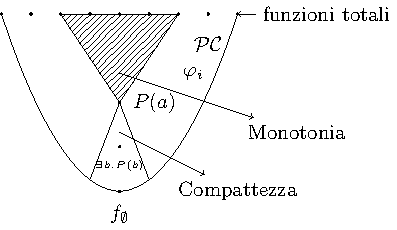
\includegraphics{img/ExtensionHierarchy.pdf}
    \caption{Una proprietà $P$ è monotona se tutte vale per tutte le estensioni di una funzione $a$
    per cui vale. È compatta se vale per una qualche restrizione finita $b$ di $a$}
\end{figure}

\newpage

Vediamo ora alcuni esempi di proprietà e chiediamoci quali sono compatte e quali monotone (e quali
entrambe).
\begin{itemize}
    \item $P(i) = ``\phii$ è totale''. È monotona? Sì. È compatta? No.
    \item $P(i) = ``\phii$ non è totale''. È monotona? No. È compatta? Sì.
    \item $P(i) = ``4 \in \cod(\phii)$''. È monotona? Sì. È compatta? Sì.
    \item $P(i) = ``\cod(\phii) = {4}$''. È monotona? No. È compatta? Sì.
\end{itemize}

Dimostreremo che monotonia e compattezza sono condizioni necessarie ma non sufficienti per la
semidecidibilità.

Prendiamo $P(i) = ``\dom(\phii)$ finito''. È monotona? No. È compatta? Sì. Per il complementare? È
monotono? Sì. È compatto? No.

%Prendiamo $P(i) = ``\dom(\phii)$ infinito e $\comp{\dom(\phii)}$ finito (?)''. È monotona? No. È
%compatta? No.

Una proprietà come $P(i) = `` \phii$ è primitiva ricorsiva'' non è neppure semidecidibile, oltre a non
essere decidibile per il teorema di Rice. Il motivo è che $P(i)$ non è compatta: il formalismo
primitivo ricorsivo mi permette di definire solo funzioni totali.

\subsection{Il teorema di Rice-Shapiro}

I nomi di questo teorema variano nella letteratura. Per noi è il teorema di Rice-Shapiro.

\begin{figure}[h]
    \centering
    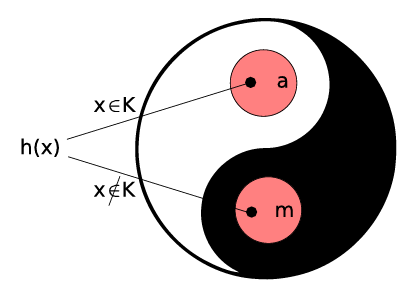
\includegraphics[scale=0.5]{img/YinYang.jpg}
    \caption{Visualizzazione della dimostrazione del teorema di Rice}
\end{figure}

\newpage

Il simbolo dello yin-yang mi deve sottolineare l'impossibilità di separare le due aree, perché le
due cose che sto tentando di separare sono processi in movimento che continuamente si trasformano
nell'una e nell'altra. Non posso operare una distinzione tra le due.

I due cerchi rappresentano degli intorni che non cambiano, che appartengono all'altra area. Da un
punto di vista topologico sono due aperti. Due aperti non possono dividere uno spazio, perché il
complementare di un aperto è un chiuso.

Possiamo immaginare un cerchio come un intorno di tutti i programmi che hanno lo stesso
comportamento di un certo programma. Se cerchiamo di dividere l'insieme di tutti i programmi in due
spazi non possiamo aspettarci di poterlo fare in modo algoritmico. Questo è il succo del teorema
di Rice. La proprietà di estensionalità, che è una proprietà di chiusura, non ci permette di
fare questa divisione.

Nella mia dimostrazione cerco un $s$ che mi permette di trovare una funzione che si comporta come
$a$ o $m$ a seconda del comportamento di $\phii(i)$. Questo lo posso fare, è più debole di
chiedere che $s(i)$ mi restituisca $a$ o $m$ a seconda del comportamento di $\phix(x)$ e sfrutta
l'estensionalità. La prima cosa posso calcolarla, la seconda no.

\begin{thm}
    \textbf{Teorema di Rice-Shapiro. }Sia $A$ un insieme estensionale. Se $A$ è r.e. allora:
    \begin{itemize}
        \item $A$ è monotono
        \item $A$ è compatto
    \end{itemize}
\end{thm}
\begin{proof}
    La monotonia mi dice che $\forall i,j$ se $i \in A$ e $\phii \subseteq \phij$ allora $j \in
    A$. Supponiamo che $A$ sia estensionale e r.e. Supponiamo che $A$ non sia monotono. Allora
    devono esistere $i,j$ tali che $i \in A$, $\phii \subseteq \phij$ e $j \notin A$. Proveremo a
    costruire un programma che si comporta come $i$ in un caso e come $j$ nell'altro caso.
    Costruiamo $h$ totale e calcolabile che vogliamo si comporti come $i$ se $\phix(x) \diverges$,
    come $j$ se $\phix(x) \converges$. Supponiamo di averla già: vedremo poi se possiamo
    calcolarla. Avremmo che $\phix(x) \in \comp{K} \iff h(x) \in A$. L'implicazione inversa di questo
    $\iff$ può essere dimostrata dimostrando $\lnot B \implies \lnot A$. Ma questo vuol dire che se
    $A$ fosse semidecidibile avrei un modo per calcolare, in modo semidecidibile, l'appartenenza a
    $\comp{K}$. 

    Tornando alla definizione del programma che calcola $h$, con s-m-n passiamo a $\phi_{h(x)} = g(x,y)
    = \phii(y) || (\phix(x)\phij(y))$. Questo programma ha lo stesso comportamento di $j$ anche se
    $\phix(x)$ converge e termina prima $\phii(y)$ perché $j$ è un'estensione di $i$. 

    Questa dimostrazione non è costruttiva. È costruttiva invece la dimostrazione per
    contraddizione: $A$ non monotono $\implies A$ non r.e.

    Questa dimostrazione implica, come corollario, il teorema di Rice.

    Passiamo alla compattezza. Questa mi dice che $\forall i, i \in A \implies \exists j, \phij \subseteq
    \phii, \phij$ è finita, $j \in A$.

    Andiamo nuovamente per assurdo. Andiamo a negare la compattezza di $A$: $\exists i, i \in A
    \forall j, \phij \subseteq \phii, \phij$ è finita $\implies j \notin A$.

    Vogliamo costruire una funzione parametrica in $x$ tale che si comporti come $i$ se $\phix(x)
    \diverges$ e come una qualsiasi restrizione finita di $i$ quando $\phix(x) \converges$. La
    conclusione della dimostrazione è identica a quella della monotonia, quindi concentriamoci su
    $h$. 

    Utilizzando s-m-n abbiamo $\phi_{h(x)} = g(x,y)$, con
    \begin{equation*}
        g(x,y) =
        \begin{cases}
            \case{\phii(y)}{se $T^{3}(x,x,y)$ = False}\\
            \case{\diverges}{se $T^{3}(x,x,y)$ = True}
        \end{cases}
    \end{equation*}

    Analizziamo il comportamento di questo programma. Ipotizziamo che $\phix(x)$ sia divergente.
    Siamo nel primo caso, quindi il comportamento del mio programma è identico a quello di $\phii$.
    Se $\phix(x)$ converge invece ad un certo punto $T$ mi restituirà True e da lì in poi la
    risposta rimarrà quella. A quel punto la mia funzione diverge. Questa corrisponde ad una
    restrizione finita di $i$: non so quanto lunga, so che esiste. Questa funzione è calcolabile,
    quindi $h$ è calcolabile, da cui l'asserto.
\end{proof}

\chapter{Teorema del punto fisso}

\section{Il teorema del punto fisso di Kleene}

I seguenti sono commenti alle slide.

\subsection{Slide 102}

La parte più a destra dell'uguale è la definizione della mia funzione $g$.

Se prendiamo per $f$ la funzione successore ho per forza che nel mio ordinamento avrò due programmi
adiacenti che si comportano nella stessa maniera. In questo modo non è possibile creare un
ordinamento tale che questo non si verifichi. La ragione fondamentale è che non ho controllo sul
comportamento dei programmi quando vado ed enumerarli.

Punti fissi e ricorsione sono fondamentalmente la stessa cosa vista da due punti di vista diversi.

La ricorsione è legata alla possibilità che nel corpo del mio programma sia visibile la funzione
che sto definendo.

Supponiamo di voler costruire un programma che stampi se stesso, ovvero che stampi il suo indice.
Per semplicità lo vogliamo costante, ovvero tale che per ogni input stampi il suo indice: $\forall
x, \phip(x) = p$.

Prendiamo $g(i,x)$ così definita:
\begin{equation*}
    g(i,x) = i
\end{equation*}

Per s-m-n otteniamo una classe di programmi costanti $\phi_{h(i)}(x)$. Questi però stampano sempre
$i$, anche se $h(i)$ è diverso da $i$, quindi non vanno bene. Sfruttando il teorema del punto fisso
abbiamo però che esiste $\phip(x) = \phi_{h(p)}(x) = p$. Di conseguenza è sufficiente prendere il
punto fisso di $h$, $p$.

Se io voglio realizzare un comportamento ricorsivo posso farlo con il teorema del punto fisso di
Kleene. Supponiamo di voler una funzione calcolabile $\phip$ tale che $\phip(x) = f(\phip(x))$, per
qualche $f$. Si può? Sì. Abbiamo che $g(i,x) = f(\phii(x))$. Ma ora per s-m-n abbiamo che questo
corrisponde a $\phi_{h(i)}(x)$. Ma ora abbiamo che $\phip(x) = \phi_{h(p)}(x) = f(\phip(x))$, se
prendiamo come $p$ il punto fisso di $h$.

In generale per punto fisso di una funzione intendiamo un input $x$ tale che $f(x) = x$. Il nostro senso
è un pò particolare perché è un punto fisso estensionale.

Il teorema dice fondamentalmente che $\forall f$ tot. calc. $\exists m, \phi_{f(m)} = \phi_{m}$.

Sfruttando questo risultato vogliamo costruire un programma che dato $i$ mi restituisca qualcosa
diverso dalla funzione $\phii$ per almeno un input, ovvero vogliamo $i$ tale che:
\begin{equation*}
    \exists x, g(i,x) \not= \phii(x).
\end{equation*}

Proviamo con $g(i,x) = \phii(x) + 1$. Per s-m-n esiste $h$ tale che $\phi_{h(i)}(x)$ identico a $g$. 
Funziona? No, se $i$ è un indice per la funzione sempre divergente. Si può fare di meglio? No, per
il teorema del punto fisso. Per qualunque trasformazione di programmi ho un punto fisso tale che
$\phi_{h(m)} = \phim$. Non ho speranza di fare una modifica effettiva ed uniforme tale che il mio
programma sia diverso da quello di partenza, e questo vale per ogni programma.

Vediamo una nuova dimostrazione del teorema di Rice basata sul teorema del punto fisso di Kleene. È
concettualmente diversa da quella vista in precedenza.

Sia $A$ un insieme estensionale. $A$ è ricorsivo sse è banale. Supponiamo per assurdo che $A$ sia
ricorsivo ma non banale, ovvero esista $i \in A$ e $j \in \comp{A}$. Posso definire $h$ tale che:
\begin{equation*}
    h(x) = 
    \begin{cases}
        \case{j}{se $x \in A$}\\
        \case{i}{se $x \notin A$}
    \end{cases}
\end{equation*}

Questa funzione sarebbe calcolabile per la ricorsività di $A$. Per il teorema del punto fisso,
essendo $h$ totle e calcolabile, deve esistere $m$ tale che $\phim = \phi_{h(m)}$. Ci chiediamo ora,
dove sta $m$? Se $m \in A$ allora stanno in $A$ anche tutti i programmi che si comportano come $m$,
tra cui anche $h(m)$. Ma se $m \in A$ allora $h(m) = j$, quindi $h(m) \notin A$. Se invece $m \notin
A$ allora $h(m) \notin A$. Ma per definizione di $h$ si ha che $h(m) = i \in A$. Ecco la mia
contraddizione.

Tutte le volte che cerchiamo programmi che dipendono, intensionalmente o meno, dall'indice del
programma che sto cercando devo fare riferimento al teorema del punto fisso.

\section{Il secondo teorema del punto fisso}

Pensiamo ora ad una funzione binaria $f(x,y)$. Possiamo generalizzare il teorema del punto fisso:
\begin{thm}
    $\forall f^{2}$ totale calcolabile $\exists s$ totale calcolabile tale che $\forall y, \phi_{f(s(y),y)} = \phi_{s(y)}$
\end{thm}
\begin{proof}
    La dimostrazione è nella slide 103
\end{proof}

\chapter{Riducibilità}

\section{\emph{Many-to-one} reducibility}

Abbiamo in precedenza visto dei procedimenti di ``riduzione'' da un insieme $A$ a $K$ per dimostare,
ad esempio, che se $A$ fosse ricorsivo anche $K$ lo sarebbe. Andiamo ora a definire formalmente la
nostra nozione di riducibilità. Ne esistono tante versioni diverse di questa nozione, noi ne
vediamo una concettualmente semplice che va sotto il nome di $m$-riducibilità. La $m$ sta per
\emph{many-to-one}; esiste ance la riduzione \emph{one-to-one}.

\begin{defn}
    Siano $A,B \subseteq \Nat$. Un insieme $A$ è $m$-riducibile a $B$ ($A \leq_{m} B$) sse
    $\exists f$ totale calcolabile tale che $x \in A \iff f(x) \in B$.
\end{defn}

Si parla di riducibilità perché possiamo ridurre la appartenenza ad $A$ all'appartenenza a $B$.
Per ogni $x$ mi basta calcolare $f(x)$ e vedere se sta in $B$ per sapere automaticamente se $x$
appartiene ad $A$. Nella \emph{one-to-one} reducibility si richiede anche che $f$ sia iniettiva. È una
nozione che troveremo molto simile nella parte di complessità, avremo solo degli ulteriori limiti
sulla complessità di $f$. 

Per dimostrare che $A \leq_{m} B$ devo fare due cose:
\begin{itemize}
    \item per prima cosa devo definire $f: \Nat \to \Nat$ totale calcolabile;
    \item dopodiché va dimostrato che è una buona funzione di riduzione, ovvero va dimostrato il
    $\iff$ della definizione.
\end{itemize}

È un esercizio creativo, cambia per diversi $A$ a $B$. La $m$-riducibilità è un ordine parziale.
Infatti $A \leq_{m} A$, con la funzione identità, e se $A \leq_{m} B$ e $B \leq_{m} C$, allora, componendo le due
funzioni di riduzione, otteniamo una funzione di riduzione da $A$ a $C$:$A \leq_{m} C$. 

Notazione: $A \leq_{m}^{f} B$ se $A$ è riducibile a $B$ attraverso la funzione $f$.

Se $A \leq_{m} B$ e $B \leq_{m} A$ allora scriveremo $A =_{m} B$. Intuitivamente sono equivalenti
dal punto di vista della riducibilità.

La nozione di riducibilità ci dà un'idea di quanto complicato è un problema. Se $A \leq_{m} B$
allora $B$ è tanto difficile quanto lo è $A$. Quanto fine è la mia misurazione dipende dalla potenza
della mia nozione di riducibilità. Se la mia nozione di riducibilità non ha troppe pretese rischio
di passare da un problema ricorsivo ad uno ricorsivamente enumerabile, e di avere molte riduzioni
possibili non molto significative.

Tutti i problemi ricorsivi sono mutuamente riducibili ad esempio. Infatti supponiamo $x \in A \iff
f(x) \in B$. A sto punto se $B$ è ricorsivo ovviamente posso decidere l'appartenenza ad $A$, e
quindi $A$ è ricorsivo. Se invece $B$ è r.e. allora, per lo stesso motivo, anche $A$ risulta essere
r.e.

L'altra implicazione non è vera. È possibile passare da un problema ricorsivo ad uno
ricorsivamente enumerabile. Il minore o uguale ha il significato intuitivo di ``$A$ non è più
difficile di $B$''.

Supponiamo di avere due insiemi ricorsivi non banali. Mostriamo che sono sempre mutuamente
riducibili l'uno all'altro. Dimostriamo solo $A \leq_{m} B$; il verso opposto usa le stesse ipotesi.
Esistono allora $b_{1} \in B$ e $b_{2} \in \comp{B}$. È banale costruire ora $f(x)$ tale che:
\begin{equation*}
    f(x) =
    \begin{cases}
        \case{b_{1}}{se $x \in A$} \\
        \case{b_{2}}{se $x \notin A$}
    \end{cases}
\end{equation*}

È una funzione totale calcolabile? Sì. Vale il sse della definizione di riducibilità? Anche, e si
vede quasi subito. È importante l'ipotesi di non banalità di $A$ e $B$. Non abbiamo usato l'ipotesi di
ricorsività di $B$. Se $B$ è un qualsiasi insieme non banale posso ridurre $A$ a $B$. Senza altre ipotesi
potrei non essere in grado di tornare indietro.

Prendiamo un insieme non ricorsivo come $K$ e supponiamo che $K$ sia riducibile ad $A$. Cosa abbiamo
concluso? Che $A$ non è ricorsivo. Analogamente se $\comp{K} \leq_{m} A$ allora $A$ non è r.e.

Abbiamo infine che $A \leq_{m} B \iff \comp{A} \leq_{m} \comp{B}$.

\section{Completezza}

Passiamo ora alla nozione di completezza. Di solito è relativa ad una classe di problemi. Qua siamo
interessati alla classe dei problemi semidecidibili.
\begin{defn}
    Diciamo che un certo problema $B$ è completo (per i problemi r.e.) se
    \begin{itemize}
        \item $B$ è r.e.
        \item $\forall A$, se $A \in \RE$, allora $A \leq_{m} B$
    \end{itemize}
\end{defn}

Potrei definire la stessa nozione per altre classi di problemi.

Il primo punto che ci interessa è, esistono dei problemi completi? La risposta è sì. Prendiamo ad
esempio $K_{1} = \set{<x,y> \mid \phix(y) \converges}$. È banalmente semidecibile. È completo? Supponiamo
che $A$ sia r.e. Esiste quindi il semidecisore di $A$, $s_{A}$. Supponiamo che sia il programma di
indice $a$ nella mia enumerazione dei programmi: $\phi_{a}(x)$. Quindi $x \in A$ sse $\phia(x) \converges$
sse $<a,x> \in K_{1}$. La funzione $f$ che mi interessa è la funzione che mappa $x$ nella coppia
$<a,x>$ : $x \mapsto <a,x>$.

Ne esistono altri? Si, ad esempio $K$ è completo. Si può dimostrare direttamente. Noi però
dimostreremo che $K \equiv_{m} K_{1}$. È facile vedere che $K \leq_{m} K_{1}$. La mia $f$ è quella tale
che $x \mapsto <x,x>$. Abbiamo che $x \in K \iff \phix(x)\converges \iff <x,x> \in K_{1}$.

La parte $K_{1} \leq_{m} K$ è un pò più tricky. Vogliamo catturare un comportamento puntuale sulla
diagonale. Questo è difficile; possiamo piuttosto catturare un comportamento uniforme che valga
ovunque, e che quindi in particolare valga anche per la diagonale.

Sia $f$ tale che
\begin{equation*}
    f(x,y,z) =
    \begin{cases}
        \case{1}{se $\phix(y) \converges$} \\
        \case{\diverges}{altrimenti}
    \end{cases}
\end{equation*}

Utilizzo ora s-m-n sulla coppia $<x,y>$: esiste $\phi_{s(x,y)}(z)$ con lo stesso comportamento. La mia
funzione $s$ è quella che cerco (questo è il mio claim).

Supponiamo che $(x,y) \in K_{1}$. Allora $\forall z \phi_{s(x,y)}(z) \converges$. In particolare
converge anche sulla diagonale. In particolare $\phi_{s(x,y)}(s(x,y)) \converges$, e qindi $s(x,y) \in
K$. Inoltre $(x,y) \notin K_{1} \implies \forall z \phi_{s(x,y)}(z) \diverges \implies
\phi_{s(x,y)}(s(x,y)) \diverges \implies s(x,y) \notin K$.

Come conseguenza abbiamo che tutti gli insiemi completi sono mutuamente riducibili: $A$ e $B$ completi
$\implies A \equiv_{m} B$.

\section{Insiemi produttivi e creativi}

Cerchiamo ora di dare altre caratterizzazioni degli insiemi completi. Vediamo se hanno delle
proprietà interessanti. Una proprietà curiosa è la creatività.

\begin{defn}
    Sia $A \subseteq \Nat$. $A$ è produttivo se esiste $f$ totale calcolabile, detta funzione di
    produzione, tale che comunque prendo un sottoinsieme $W_{i} \subseteq A$ , si ha che $f(i) \in A
    \setminus W_{i}$.
\end{defn}

Ricordiamo che $W_{i}$ è la numerazione dei sottoinsiemi r.e. basata sul dominio di convergenza
della funzione $i$ della mia numerazione delle funzioni calcolabili.

Cos'è che produce la funzione di produzione? Uno potrebbe essere interessato a dare una
approssimazione r.e. di questi insiemi. Cosa intendiamo? Dare un sottoinsieme di $A$ ricorsivamente
enumerabile. $f$ mi produce una dimostrazione, per ogni approssimazione, dell'incompletezza della
mia approssimazione in funzione dell'algoritmo con cui enumeriamo i programmi. $f$ è unica,
definita a prori dall'insieme $A$. Questo concetto è stato suggerito dai problemi di incompletezza
logica.

C'è una caratterizzazione degli insiemi completi attraverso la produttività.

%\begin{defn}
%    Sia $A \subseteq \Nat$. $A$ è produttivo sse $\exists f$ totale calcolabile tale che $\forall
%    i, W_{i} \subseteq A \implies f(i) \in A \setminus W_{i}$.
%\end{defn}

Possiamo pensare ad $A$ come all'insieme delle formule vere dell'aritmetica. Quando costruiamo un
sistema formale per ragionare sull'aritmetica, ovvero un sistema di assiomi fondamentalmente e le regole
logiche per passare alle conseguenze logiche degli assiomi, avremo, per il teorema di incompletezza,
che ci saranno sempre formule vere che non sono però dimostrabili nel sistema formale.

È una tecnica simile alla diagonalizzazione.

Un insieme produttivo non è, per sua natura, r.e.; altrimenti potrei approssimarlo con l'insieme
stesso.

\begin{defn}
    Un insieme $A \subseteq \Nat$ è creativo se $A$ è r.e. e $\comp{A}$ è produttivo.
\end{defn}

Non tutti gli insiemi produttivi hanno un complementare r.e.

$K$ è un esempio di insieme creativo. Per dimostrarlo ci manca solo da dimostrare che $\comp{K}$ è
produttivo. Questo è semplice però perché la funzione di produzione per $\comp{K}$ è la funzione
identità.

Sia $W_{i} \subseteq \comp{K}$. Dobbiamo dimostrare che $i \in \comp{K}$ e $i \notin W_{i}$.

Per la prima appartenenza andiamo per assurdo. Supponiamo che $i \in K$. Allora $i \in W_{i}$. Ma
essendo $W_{i}$ sottinsieme di $\comp{K}$ si ha $i \in \comp{K}$, il che è assurdo. Quindi $i \in
\comp{K}$.

Per la seconda appartenenza andiamo nuovamente per assurdo. $i \in W_{i} \implies i \in K \implies
\absurd \implies i \notin W_{i}$.

\section{Relazione tra creatività e completezza}

Nota: La seguente è l'ultima dimostrazione richiesta per l'orale.

Da qui in poi verrà usato il simbolo $\leq$ sottintendendo $\leq_{m}$. Vediamo un risultato
importante per gli insiemi produttivi

\begin{thm}
    Un insieme $A \subseteq \Nat$ è produttivo $\comp{K} \leq A$.
\end{thm}

Questo implica come corollario che $A$ è creativo sse $A$ è r.e. e $K \leq A$. Di conseguenza
insiemi creativi ed insiemi completi coincidono.

\begin{proof}
    Dimostriamo il primo teorema. Abbiamo i due versi del $\iff$ da dimostrare. Il più semplice dei due è
    quello inverso: $\comp{K} \leq A \implies A$ è produttivo.

    Sia quindi $\comp{K} \leq A$. Sia $f$ la funzione di riducibilità di $\comp{K}$ in $A$. Sappiamo anche che
    $\comp{K}$ è produttivo, con funzione di produzione uguale ad \textit{Id}. L'idea è di ritornare a
    $\comp{K}$ da $A$ attraverso $f$. Dopodiché, utilizzando la funzione di produzione di $K$,
    troviamo un nuovo elemento che, attraverso alla funzione $f$, sta in $A$ e non in $W_{i}$.

    Ricordiamo che la controimmagine di una insieme $A$ attraverso una funzione $f$ è definita come
    $f^{-1}: \Nat \to \Nat$ tale che $f^{-1}(A) = {x | f(x) \in A})$.

    Consideriamo $f^{-1}(W_{i})$, la controimmagine di $W_{i}$ via $f$. Abbiamo che sicuramente
    $f^{-1}(W_{i}) \subseteq \comp{K}$ e che è r.e. È importante che $f$ sia totale. Se calcolo la
    controimmagine di un insieme attraverso una funzione parziale potrei ottenere un insieme non
    ricorsivamente enumerabile. L'indice di $f^{-1}(W_{i})$ può essere calcolato in maniera
    effettiva attraverso una funzione totale calcolabile $h$.  Abbiamo quindi che corrisponde a
    $W_{h(i)}$. Pensiamo alla funzione $\phii(f(x)) = \phi_{h(i)}(x)$ per s-m-n. Dove sta $h(i)$?
    Sta in $\comp{K}$ ma non in $f^{-1}(W_{i})$, essendo $\comp{K}$ produttivo con funzione di
    produzione uguale a \textit{Id}. Passando quindi, attraverso $f$, al corrispondente in $A$
    ($f(h(i))$) abbiamo che sta in $A$ ma non in $W_{i}$. Quindi $A$ è produttivo.

    La dimostrazione poteva essere fatta con un altro insieme produttivo. In particolare, se $B$ è
    produttivo e $B \leq A$ allora $A$ è produttivo.

    Passiamo ora al verso opposto: $A$ produttivo $\implies \comp{K} \leq A$.

    Sia $A$ produttivo e sia $f$ la funzione di produzione per $A$. Vado alla ricerca di $W_{s(i)}$
    tale che:
    \begin{equation*}
        W_{s(i)} =
        \begin{cases}
            \case{\{f(s(i))\}}{se $i \in K$} \\
            \case{\emptyset}{se $i \in \comp{K}$}
        \end{cases}
    \end{equation*}

    Non sappiamo, per ora, se esiste $s$; supponiamo però di poterla definire. Per dimostrare la
    sua esistenza ricorreremo al teorema del punto fisso.

    Vogliamo dimostrare che $i \in \comp{K}$ sse $f(s(i)) \in A$. Supponiamo che $i \in \comp{K}$.
    Allora $W_{s(i)} = \emptyset \subseteq A$. Posso applicare la produttività e quindi concludere
    che $f(s(i)) \in A$.

    Supponiamo che $i \in K$. Allora $W_{s(i)} = \{f(s(i))\}$. Supponiamo per assurdo che $f(s(i)) \in A$.
    Allora $W_{s(i)} \subseteq A$. Sfruttando la produttività avremmo che $f(s(i)) \in A$ e che
    $f(s(i)) \notin W_{s(i)}$. Ma questo è assurdo. Perciò $f(s(i)) \notin A$.

    La dimostrazione è incompleta, manca la dimostrazione dell'esistenza di $s$. Ci serve il secondo
    teorema di ricorsione. Partiamo da $g(i,z,x)$ tale che:
    \begin{equation*}
        g(i,z,x) =
        \begin{cases}
            \case{1}{se $\phi(i) \converges \land x = f(z)$} \\
            \case{\diverges}{se $\phii(i) \diverges$}
        \end{cases}
    \end{equation*}
    
    Per s-m-n esiste $h(i,z)$ tale che $\phi_{h(i,z)}(x)$ ha lo stesso comportamento. Esiste ora $s$ tale che
    $\forall i \phi_{s(i)} = \phi_{h(i,s(i))}$. Abbiamo quindi che
    \begin{equation*}
        \phi_{s(i)}(x) = \phi_{h(i,s(i))}(x) = g(i,s(i),x) =
        \begin{cases}
            \case{1}{se $\phii(i) \converges \land x = f(s(i))$} \\
            \case{\diverges}{se $\phii(i) \diverges$}
        \end{cases}
    \end{equation*}
\end{proof}

\begin{proof}
    Dimostriamo il corollario. Sia $A$ creativo. Allora $A$ è r.e. e $\comp{A}$ è produttivo. Allora
    $\comp{K} \leq \comp{A}$. Ma questo implica che $K \leq A$.

    Sia $A$ r.e. e completo. Allora $K \leq A$. Allora $\comp{K} \leq \comp{A}$, quindi $\comp{A}$ è
    produttivo, di conseguenza $A$ è creativo.
\end{proof}

\section{Insiemi r.e. non completi}

Supponiamo di avere un insieme $A$ r.e. Vogliamo dimostrare che $A$ non è ricorsivo. Posso condurre
questa dimostazione sempre dimostrando che $K \leq A$? Limitatamente agli insiemi creativi/completi
allora sì. Il punto è, esiste un insieme r.e. non creativo? Questo va sotto il nome di problema di
Post. È rimasto aperto per un certo numero di anni e veniva considerato un problema difficile.  È
un analogo del problema $\NPClass$ vs $\PClass$. Nella teoria della complessità però si sà molto di meno. È più
facile per un insieme r.e. essere completo che il contrario.

Per rispondere a questa domanda abbiamo bisogno di due risultati intermedi.

Sia $A$ un insieme r.e. infinito. Esiste $B$ ricorsivo infinito sottoinsieme di $A$? Sì. Una
caratterizzazione degli insiemi ricorsivi è che sono enumerabili in maniera crescente. Se prendo
l'enumerazione $f$ di $A$ e la ``taglio'' in pezzetti crescenti e li uso per definire la mia
enumerazione di $B$ ho che questa è crescente, e quindi $B$ è ricorsivo infinito. Più
precisamente, la mia enumeraziona $g$ di $B$ sarà fatta nel modo seguente, se $f$ è la mia
enumerazione di $A$: $g(0) = f(0)$ e $g(x+1) = f(\mu y. f(y) \geq g(x))$.


Se vediamo l'estrazione di sottoinsiemi come un'operazione di focalizzazione possiamo focalizzarci
su insiemi di complessità desiderata 

//TODO RIPORTARE FIGURA DAL QUADERNO
(vedi figura sul quaderno azzurro).

Sia $A$ un insieme ricorsivo infinito. Allora $\exists B$ r.e. non ricorsivo tale che $B \subseteq
A$.

Consideriamo una funzione di enumerazione $f$ per $A$ iniettiva. Consideriamo l'insieme $B$ così
definito:
\begin{equation*}
    B = \set{f(\phii) \mid i \in \Nat}
\end{equation*}
$B$  è l'immagine di $K$ via $f$.

Abbiamo che $B$ è sottoinsieme di $A$ e che $B$ è r.e.; è facile da vedere. Dobbiamo dimostrare
che $B$ non è decidibile. Questo è vero perché altrimenti $K$ sarebbe decidibile. Per vederlo è
sufficiente dimostrare che vale il sse $i \in K \iff f(\phii(i)) \in B$. È facile.

Noi abbiamo intrapreso questo discorso perché cercavamo un insieme r.e. non completo. Una
proprietà interessante degli insiemi produttivi è che ogni insieme produttivo contiene un
sottoinsieme r.e. infinito.

\begin{thm}
    Sia $A \subseteq \Nat$ produttivo. Allora $\exists B$ r.e. infinito tale che $B \subseteq A$.
\end{thm}

È una proprietà cruciale che ci serve perché costruiremo un insieme infinito che non contiene
alcun sottoinsieme r.e. In pratica abbiamo un insieme tale che qualsiasi suo sosttoinsieme infinito
è talmente caotico da non essere nemmeno r.e.

\begin{proof}
    Per la dimostrazione useremo la produttività. Proviamo ad approssimare $A$. Inizieremo con l'insieme
    vuoto. Per la produttività esiste $a \in A$. Ora nella mia approssimazione includo pure $a$. Per
    produttività esiste $a' \in A$ fuori dalla mia approssimazione, e continuo così all'infinito. Questo
    procedimento è costruttivo e mi crea la mia approssimazione r.e. di $A$.

    Questo procedimento ha un analogo con il tentativo di approssimare l'insieme delle conseguenze
    di un insieme di assiomi. Per l'incompletezza esiste una formula che non è dimostrabile dal mio
    sistema formale. A questo punto potrei aggiungere la validità di questa formula al mio sistema
    formale e crearne uno nuovo. Ma a questo punto ho un nuovo sistema formale, e il ragionamento
    precedente si applicherebbe identicamente. Quindi non potrò mai avere un insieme che contenga
    tutte le conseguenze dei miei assiomi.

    Vogliamo dimostrare che $W_{h(i,a)} = W_{i} \cup {a}$. Più precisamente vogliamo dimostrare che
    esiste un modo effettivo per calcolare un insieme r.e. ottenibile mediante estensione di $W_{i}$
    con $a$. $W_{h(i,a)}$ è il dominio di una certa funzione $\phi_{h(i,a)}$. Vogliamo quindi che
    $\phi_{h(i,a)}(x) = g(i,a,x) = \phii(x)|(x = a)$. In pratica voglio che converga se $x = a$ oppure se
    $x$ fa parte del dominio di $\phii$. $g$ è effettivamente calcolabile e ho quindi un metodo effettivo
    per calcolare $W_{h(i,a)}$ ogni volta.

    Possiamo ora costruire la mia sequenza di approssimazione. $W_{m} = \emptyset$. Sia $s$ la
    funzione di produzione per $A$. Ho che $s(m) \in A \setminus W_{m}$. Passo quindi a
    $W_{h(m,s(m))=m_{1}} = \set{s(m)}$. La mia seconda approssimazione sarà $W_{h(m_{1},s(m_{1}))} =
    {s(m),s(m_{1})}$.

    Se definiamo $\textit{next}(x) = h(x,s(x))$ possiamo definire $g(x) = next^{x}(m_{0})$ e abbiamo
    che $B$ è uguale al codominio di $g$.
\end{proof}

\subsection{Complessità di Kolmogorov}

Se noi vogliamo trasmettere un'informazione, diciamo il numero $n$, abbiamo due modi per farlo: uno
è trasmettere direttamente $n$, ad esempio con la sequenza di bit che rappresnta $n$, che ha un
costo che dipende da $n$; un'altra possibilità è trasmettere un modo per costruire $n$. Ad esempio un
algoritmo.

In particolare, immaginiamo un programma $i$ tale che $\phii(0) = n$. Posso trasmettere direttamente
$i$. Qual è più conveniente? Intuitivamente quello più piccolo. Confronto $i$ con $n$. Se $i$ è più
piccolo trasmetto $i$, altrimenti trasmetto $n$.

\begin{defn}
    La complessità di Kolmogorov di $n$, $K(n)$, è il minimo $i$ tale che $\phii(0) = n$ (=
    $\min\set{i \mid \phii(0) = n}$).
\end{defn}

È una astrazione di una problematica reale legata alla comprimibilità delle informazioni.

Il mio confronto è tra $n$ e $K(n)$.

\subsection{Numeri random}

\begin{defn}
    $n \in \Nat$ è un numero random se $n \leq K(n)$.
\end{defn}

Dobbiamo pensare a $n$ come alla sua espansione decimale: una stringa di bit.

Perché usiamo la nozione di \textit{Random} per descrivere questa caratteristica? Perché è una
idea del concetto. Se ci fosse una grande regolarità nella stringa per $n$ è chiaro che posso creare
un programma piccolino che lo generi. Si parla di dati lawful o lawless. I dati che seguono una
regola non saranno random. Se sono random sono talmente disordinati che non riesco a dare nessun
metodo generativo più breve dei dati stessi. È un approccio formale alla nozione di random legata
alla comprimibilità del dato.

Come l'abbiamo vista la nostra nozione di ``casualità'' dipende dalla nostra enumerazione dei programmi.
Per numeri grandi però non dovrebbe cambiare niente se cambia la numerazione.

Un'altra questione è che la nostra nozione di random va bene per sequenze finite. Noi in generale
vorremmo idealmente una nozione che valga per sequenze infinite. In questo contesto però ci è
sufficiente.

La randomicità di un numero è decidibile? È semidecidibile? Potrei pensare di fare una ricerca
limitata ad $n$ per un programma che genera $n$. Il problema è che le mie funzioni sono parziali
calcolabili, potrebbero divergere. Quindi sembrerebbe che la risposta sia no.

Cosa possiamo però semidecidere? Se un numero non è random. Se $\Rand$ è l'insieme dei numeri random
allora abbiamo che $\comp{\Rand}$ è semidecidibile. La nostra congettura è che $\Rand$ non sia nemmemno
semidecidibile.

Abbiamo un altro modo per dimostrare quanto detto su $\comp{\Rand}$, oltre al lanciare in parallelo
tutti i $\phii$ e aspettare che uno di essi termini. Lanciamo $\phii(0)$ e vediamo se è uguale a
$n$. Se $\phii(0) = n$ e $i < n$ allora restituisco $n$, altrimenti divergo. Questa funzione
$g(<i,n>)$ è una funzione di numerazione parziale che dà fuori numeri che non sono random. Prima o
poi tutti i numeri non random verranno enumerati.

Il nostro claim è che l'insieme dei numeri random non è produttivo.

Vogliamo dimostrare che $\Rand$ non è produttivo. Lo dimostriamo facendo vedere che $\Rand$ non contiene
nessun sottoinsieme r.e. infinito.

Noi dimostriamo ciò dimostrando che in $\Rand$ non ci sia nessun sottoinsieme ricorsivo infinito.
Grazie ai risultati dimostrati in precedenza è equivalente.

Supponiamo, per assurdo, che $A$ sia ricorsivo e che $A \subseteq \Rand$. Definiamo $g(i,x) = \mu n, n \in A$
e $n > i$. L'idea è che $A$ è ricorsivo, e quindi possiamo decidere $n \in A$, e possiamo andare alla
ricerca del più piccolo $n$ maggiore di $i$. Questa funzione è calcolabile e per s-m-n abbiamo che
possiamo calcolarla con $\phi_{h(i)}(x)$. 

Esitste $p$ tale che $\phi_{p}(x) = \phi_{h(p)}(x) = \mu n, n \in A$ e $n > p$, per il teorema del
punto fisso. Ora mi chiedo $\phip(0)$ è random? Dovrebbe essere random, dato che l'output sta in $A
\subseteq \Rand$. Ma al tempo stesso $\phip(0)$ è generato da $p$ e, per costruzione, $p < \phip(0)$. E
quindi sarebbe non random. Assurdo.

Questa parte è legata al paradosso di Berry.

Un insieme che non contiene insiemi r.e. infiniti è detto immune e il suo complementare è detto
semplice.

Abbiamo quindi che l'insieme dei numeri random non è produttivo. Di conseguenza l'insieme $\comp{\Rand}$ 
è r.e. non ricorsivo e non creativo, ovvero non completo.

\chapter{La gerarchia aritmetica}

\section{Aritmetica e incompletezza}

Quando vogliamo parlare di qualcosa abbiamo bisogno di un linguaggio. Partiamo da un insieme di
segni.

Il linguaggio dell'aritmetica è il linguaggio del primo ordine basato sulla
seguente segnatura:
\begin{equation*}
    0,S,+,\cdot,=
\end{equation*}

Indichiamo con $\bar{n}$ il termine che rappresenta il numero $n$. Occhio a non fare confusione tra
termine che rappresenta un numero e numero stesso. Ad esempio 3 (il numero) vs $S(S(S(0))))$ (il
termine per il numero 3).

\begin{defn}
    $A \subseteq \Nat^{k}$ si dice aritmetico se esiste una formula aritmetica
    $\psi(x_{1},\dotsc,x_{k})$ tale che
    \begin{equation*}
        (n_{1},\dotsc,n_{k}) \in A \iff \StdNat \models \psi[\bar{n_{1}}/x_{1},\dotsc,\bar{n_{k}}/x_{k}]
    \end{equation*}
    ovvero $\psi(x_{1},\dotsc,x_{k})$ è vera sui numeri naturali. Diremo in questo caso che $\psi$ è una
    descrizione aritmetica di $A$.
\end{defn}

Ad esempio, l'insieme dei numeri primi è aritmetico, in quanto puo` essere
descritto dalla seguente formula aritmetica:
\begin{equation*}
    \psi(n) = n \geq 2 \land \forall y, 1 < y \land y < n \implies \forall z, y \cdot z \not= n
\end{equation*}

Non tutti gli insiemi sono aritmetici. I possibili sottoinsiemi di $\Nat$ sono più che numerabili,
non posso aspettarmi di descrivere tutti questi nell'aritmetica.

Gli insiemi aritmetici sono chiusi rispetto alle operazioni di unione, intersezione
e complementazione.

\begin{defn}
    Una funzione $f$ si dice aritmetica se il suo grafo è un insieme aritmetico.
\end{defn}

Le seguenti funzioni sono aritmetiche:
\begin{itemize}
    \item la costante 0, descritta dalla formula $\psi(y) := y = 0$;
    \item la funzione unaria successore, descritta dalla formula $\psi(x,y) := y = S(x)$;
    \item la funzione binaria somma, descritta dalla formula $\psi(x_{1},x_{2},y) := y = x_{1} + x_{2}$;
    \item la funzione binaria prodotto, descritta dalla formula $\psi(x_{1},x_{2},y) := y = x_{1} \cdot x_{2}$;
    \item la proiezione $k$-aria $\pi_{i}^{k}$, descritta dalla formula $\psi(x_{1},x_{2},\dotsc,x_{k},y) :=
    y = x_{k}$;
\end{itemize}

È ragionevole chiedersi se anche le funzioni aritmetiche sono chiuse rispetto ai metodi tipici per
comporre le funzioni: definire nuove funzioni a partire da quelle esistenti.

Il primo modo che ci può venire in mente è la composizione di funzioni.

\begin{lem}
    La composizione di funzioni aritmetiche è aritmetica.
\end{lem}
\begin{proof}
    Sia $f(x) = g(h(x))$ e siano $\psi_{g}(x,y)$ e $\psi_{h}(x,y)$ le descrizioni aritmetiche di $g$
    e $h$.

    Definiamo
    \begin{equation*}
        \psi_{f}(x,z) = \exists y, \psi_{h}(x,y) \land \psi_{g}(y,z)
    \end{equation*}

    Si può dimostrare che $\psi_{f}$ è una descrizione aritmetica di $f$.
\end{proof}

Altre operazioni di definizione di nuove funzioni tipiche sono la ricorsione primitiva e la minimizzazione.

Se abbiamo la minimizzazione (che corrisponde circa ad un while) possiamo avere subito la ricorsione
primitiva (che corrisponde ad un for).

\begin{lem}
    Una funzione definita per minimizzazione di una funzione aritmetica è ancora aritmetica.
\end{lem}
\begin{proof}
    Sia
    \begin{equation*}
        f(x) = \mu y, (g(x,y)=0)
    \end{equation*}
    e supponiamo che $\psi_{g}$ sia una descrizione aritmetica di $g$. $f$ è descritta dalla
    seguente formula:
    \begin{equation*}
        \psi_{f}(x,y) = \psi_{g}(x,y,0) \land \forall z, z < y \implies \exists m, (\psi_{g}(x,z,m)
        \land m \not= 0)
    \end{equation*}
\end{proof}

Possiamo prendere la descrizione delle funzioni come la specifica di un programma. Ci poniamo quindi
il problema di quali funzioni sono specificabili.

\begin{thm}
    Tutte le funzioni calcolabili sono aritmetiche.    
\end{thm}

Questo è conseguenza del fatto che ogni funzione calcolabile può essere espressa in un formalismo che
contiene somma, prodotto, costanti, proiezioni ed è chiuso per composizione e minimizzazione.

Mi serve anche l'uguaglianza nel mio formalismo.

\begin{thm}
    Ogni insieme ricorsivamente enumerabile è aritmetico.
\end{thm}
\begin{proof}
    Se $A$ è r.e. esiste $f$ parziale calcolabile tale che $A = \dom(f)$. Sia $\psi_{f}(x,y)$ una
    descrizione aritmetica di $f$. Allora:
    \begin{equation*}
        n \in A \iff \StdNat \models \exists y, \psi(\bar{n},y)
    \end{equation*}
    e dunque $\psi_{A}(x) = \exists y, \psi(x,y)$ è una descrizione aritmetica di $A$.
\end{proof}

\begin{thm}
    L'insieme delle formule aritmetiche vere non è ricorsivamente enumerabile.
\end{thm}
\begin{proof}
    Sia $\set{\psi_{n}}_{n \in \Nat}$ una enumerazione effettiva delle formule aritmetiche in una
    variabile. Consideriamo l'insieme $A$ così definito
    \begin{equation*}
        n \in A \iff \StdNat \models \lnot \psi_{n}(\bar{n})
    \end{equation*}
    Se la verità aritmetica fosse semidecidibile allora $A$ sarebbe r.e. Dunque $A$ dovrebbe essere
    aritmetico e dovrebbe esistere una formula $\psi_{a}$ per cui
    \begin{equation*}
        n \in A \iff \StdNat \models \lnot \psi_{a}(\bar{n})
    \end{equation*}
    Ma per $n=a$ otteniamo una contraddizione.
\end{proof}

\begin{thm}
    Ogni sistema formale aritmetico, se consistente, è incompleto (i.e. esistono formule
    aritmetiche valide ma non dimostrabili).
\end{thm}

Un sistema formale è definito da un insieme ricorsivo di assiomi e un insieme di
regole di inferenza che permettono di dedurre nuovi teoremi a partire dagli
assiomi in un numero finito di applicazioni.

Pertanto le formule aritmetiche dimostrabili costituiscono un insieme
ricorsivamente enumerabile.

Poichè le formule vere non sono r.e. esistono necessariamente delle formule
vere ma non dimostrabili.

È difficile descrivere in maniera categorica una teoria. Esistono poche teorie per cui non sia
possibile cambiare il modello e ribaltarla completamente.

\section{La gerarchia aritmetica}

L'uguaglianza tra numeri naturali è decidibile. Questo non è banale, ad esempio per i numeri reali
non è nemmeno semidecidibile l'uguaglianza; per essi è semidecidibile la disuguaglianza.

Data una formula aritmetica possiamo spostare tutti quantificatori all'inizio della formula. La mia
formula acquista quindi la forma $Q_{1} x_{1} Q_{2} x_{2} Q_{3}x_{3} \dotsc Q_{n}x_{n}P$, con $P$ senza
quantificatori e con $P$ decidibile. Se abbiamo dei quantificatori uniformi che si susseguono possiamo
collassarli. Ad esempio $\forall x_{1} \forall x_{2} \dotsc$ diventa $\forall <x_{1},x_{2}> \dotsc$. Nella
formula si parlerà poi di proiezioni della codifica al posto delle singole istanze delle variabili
collassate. Ad esempio $\textit{fst}(x)$ invece che $x_{1}$, $\pi_{n}(x)$ invece che $x_{n}$.

Nel collasso c'è un cambio di notazione. Il $\forall$ diventa $\Pi_{n}$, con $n$ uguale al numero di
inversioni $\forall$ $\exists$. Lo stesso discorso vale per $\exists$ e $\Sigma_{n}$. Ad esempio,
$\forall \exists \forall$ è di classe $\Pi_{3}$, e $\exists \forall$ è di classe $\Sigma_{2}$. Esiste poi
$\Delta_{n} = \Pi_{n} \cap \Sigma_{n}$.

Quali sono le formule $\Sigma_{1}$? Quelle semidecidibili. Perché? Perché sono proiezione
esistenziale di precidati decidibili.

Se $A \in \Sigma_{n}$ allora $\comp{A} \in \Pi_{n}$. $\Pi_{1}$ corrisponde alla classe degli insiemi
co-r.e. Come conseguenza ho che $\Delta_{1}$ è la classe degli insiemi ricorsivi.

La gerarchia degli insiemi è interessante perché dà una classificazione degli insiemi per
complessità computazionale.

Il ragionamento vale per tutti i tipi di proprietà, non solo quelle estensionali. In generale si
vuole dare una descrizione aritmetica di un programma. Da questa poi sarà possibile fare dei
ragionamenti per capire ``quanto sia difficile''. Ad esempio, sia $P(i) = ``W_{i} \text{ è
finito}$''. La sua
descrizione aritmetica sarebbe $\exists x \forall y \forall t \forall m, y \geq x \implies \lnot
T(i,y,m,t)$. Ho che $P(i) \in \Sigma_{2}$. Mi aspetto che non sia ne r.e. ne co-r.e., e in effetti non
lo è. Va comunque ricordato che l'appartenenza ad una classe non è mutalmente esclusiva. Potrei
avere proprietà $\Sigma_{2}$ che appartengono a $\Sigma_{1}$. Questo di solito accade quando i
quantificatori sono bound, che è la stessa situazione che avremmo se non esistessero.

In $\Delta_{n}$ stanno insiemi descrivibili sia con una formula in $\Pi_{n}$ che con una formula in
$\Sigma_{n}$.

\chapter{Esercizi svolti in classe}

\section{Compito Parziale Gennaio 2018}

\subsection{Esercizio 1}

\begin{enumerate}[label=(\alph*) ]
    \item Basta prendere un semidecisore per un insieme r.e. non ricorsivo. 
    \item Supponendo che $f^{-1}(A)$ non sia vuoto, dato che se è vuoto è già r.e., possiamo
    costruire una enumerazione di $f^{-1}(A)$ sfruttando il semidecisore di $A$:
    \begin{equation*}
        e_{f^{-1}(A)}(<x,t>) =
        \begin{cases}
            \case{x}{se $T(i,x,t,y) \land s_{A}(y)$}\\
            \case{a_{0}}{altrimenti}\\
        \end{cases}
    \end{equation*}
    dove $a_{0}$ è un elemento qualsiasi di $f^{-1}(A)$ e $i$ è un indice per $f$.
\end{enumerate}

%b) ho facilmente il semidecisore di f^{-1}(A): mi basta calcolare f(x). Se termina ho che x \in
%f^{-1}(A), altrimenti divergo.
% Nota personale: Ma se f termina e f(x) \notin A non dovrei divergere comunque? Ho due fonti di divergenza: f e il
% semidecisore di A

Cosa posso dire della controimmagine di un insieme $A$ attraverso una funzione $f$? 

\begin{table}[h]
    \centering
    \begin{tabular}{|c|c|c|}
    \hline
    \diagbox{$f$}{$A$} & Ricorsivo & R.E.\\
    \hline
    totale & $f^{-1}(A)$ è Ricorsivo & $f^{-1}(A)$ è r.e. \\
    \hline
    parziale & $f^{-1}(A)$ è r.e. & $f^{-1}(A)$ è r.e. \\
    \hline
    \end{tabular}
\end{table}

%f \ A    | Ricorsivo | R.E.
%--------------------------
%totale   | Ricorsivo | R.E.
%--------------------------
%parziale | R.E.      | R.E.

Questo vale in generale. Per alcuni casi particolari potrei avere situazioni più precise. Ad
esempio funzione parziale e A ricorsivo e controimmagine ricorsiva.

E dell'immagine cosa possiamo dire? L'immagine di un insieme r.e. attraverso $f$ rimane r.e.
(un'ovvietà). E se $f$ è totale e $A$ è ricorsivo? Non posso dire con certezza che l'immagine
sarà ricorsiva. Se ad esempio prendo la funzione di enumerazione di un insieme r.e. ottengo
un'immagine r.e. a partire da un insieme ricorsivo ($\Nat$).

\subsection{Esercizio 2}

La funzione di enumerazione di un insieme r.e. può sempre essere iniettiva (\ie posso enumerare
senza ripetizioni), non può essere mai crescente.

\subsection{Esercizio 3}

La specifica di $\textit{count}_{f}$ è totale, vediamo se esiste un programma che la rispetti.

Posso scegliere la mia $f$ come voglio per mostrare un controesempio nella mia dimostrazione che
$\textit{count}_{f}$ non è calcolabile.

Scegliamo per $f$ la funzione di enumerazione di $K$. $count_{f}(n) = 0 \iff n \notin K$.

\section{Esercizio 4}

Se $\phii$ fosse totale non avrei problemi, visiterei progressivamente i miei input finché non trovo
il più piccolo per cui vale quella proprietà.

La congettura è che $g$ non sia calcolabile. Costruiamo una funzione $\phi$ tale che $g$ non sia
calcolabile per $\phi$.

Sia $f(i,x)$ tale che:
\begin{equation*}
    f(i,x) =
    \begin{cases}
        \case{0}{se $x = 0$ e $\phii(i) \converges$}\\
        \case{1}{se $x \geq 1$}
    \end{cases}
\end{equation*}

Per s-m-n ho $h$ che mi curryfica la mia funzione. Ora, cosa posso dire per $g(h(i))$?

\begin{equation*}
    g(h(i)) =
    \begin{cases}
        \case{0}{se $\phii(i) \converges$}\\
        \case{1}{se $\phii(i) \diverges$}\\
    \end{cases}
\end{equation*}

\subsection{Esercizio 5}

In questo tipo di esercizi posso usare i meta-teoremi di Rice e Rice-Shapiro.

Il seguente insieme è compatto, monotono non r.e.:

\begin{equation*}
    A = \set{ i \mid W_{i} \cap \comp{K} \not= \emptyset} = \set{ i \mid dom(\phii) \cap \comp{K}
    \not= \emptyset } = \set{ i \mid \exists x, \phii(x) \converges \land \phi_{x}(x) \diverges}
\end{equation*}

Se estendo $A$ avrò sempre intersezione non vuota, quindi vale la monotonia. Se l'intersezione è diversa dal vuoto
ho $x$ che appartiene all'intersezione. Posso restringermi a quell'$x$, e quindi vale la compattezza.

$A$ non è r.e. Dato un numero $x$ esiste sempre una funzione totale calcolabile tale che $W_{h(x)}
= \set{x}$ (si costruisce con s-m-n). Ora, $h(x) \in A \iff W_{h(x)} = \set{x} \cap \comp{K} \not=
\emptyset \iff x \in \comp{K}$.

Per dimostrae che A non è r.e. posso provare a dimostrare che $\comp{K} \leq A$. Per mostrare
che $A$ non è ricorsivo cerco in genere una riduzione da $K$ ad $A$ ($K \leq A$). Va tuttavia
ricordato che non tutti gli insieri r.e. sono completi.

Vediamo una definizione del parallelo, ovvero a precisare cosa significa lanciare in parallelo due
programmi.

Definiamo:
\begin{equation*}
    (f || g)(x) =
    \begin{cases}
        \case{\diverges}{se $f(x) \diverges$ e $g(x) \diverges$} \\
        \case{f(x)}{se $f(x) \converges$ e $g(x) \diverges$} \\
        \case{g(x)}{se $f(x) \diverges$ e $g(x) \converges$} \\
        \case{\max\set{f(x),g(x)}}{se $f(x) \converges$ e $g(x) \converges$}
    \end{cases}
\end{equation*}

Questa funzione è calcolabile? Intuitivamente no: supponiamo che lanciando il nostro programma $f$ 
termini. Non possiamo determinare se $g$ divergerà, quindi non saremo mai certi di cosa restituire.

Più precisamente, scegliamo per $f$ il semidecisore di $K$ e per $g$ la funzione costante $\bm{0}$.
Abbiamo che
\begin{equation*}
    (f || g)(x) =
    \begin{cases}
        \case{1}{se $\phix(x)\converges$}\\
        \case{0}{se $\phix(x)\diverges$}\\
    \end{cases}
\end{equation*}

Sarebbe bello se, dato un programma qualsiasi, ne esistesse una estensione totale. In questo modo
potrei lavorare sempre con l'estensione e avrei una funzione totale.

La domanda è, può una data funzione $\phii$ essere estesa a una funzione totale calcolabile? La
risposta è in generale no. Esistono funzioni parziali per cui non può esistere una estensione
totale.

La funzione che consideriamo, tra le tante, è $f(x) = \phix(x) + 1$. Sia $\hat{f}$ una estensione
totale di $f$ con indice $m$ ($\phim$). Abbiamo che $\phim(m) \converges$, essendo $\phim$ totale,
ed $f(m)$ deve di conseguenza convergere, per sua definizione. Ora, $\hat{f}(m)$ dovrebbe evere lo
stesso valore di $f(m)$, essendo una sua estensione. Ma allora avremmo $\phim(m) = f(m) = \phim(m) +
1$, il che è assurdo.

Consideriamo l'insieme $A = \set{i \mid \phii \text{ è estendibile}}$. Come lo classifichiamo? Essendo una
proprietà estensionale possiamo applicare i nostri meta-teoremi. Abbiamo inoltre, grazie al
risultato precedente, che esistono funzioni non estendibili (il che non è banale). Ora
immediatamente per Rice so che $A$ non è ricorsivo. È sicuramente compatto, dato
che $f_{\emptyset}$ è estendibile banalmente. Non è invece monotono, dato che se estendo una
funzione con una estensione totale ho che quest'ultima non è più estendibile.

Classificare l'insieme $A = \set{i \mid \phii(i) = i}$. Non essendo la proprietà caratterizzante
estensionale non posso applicare Rice o Rice Shapiro. Ho che la proprietà è sicuremante
semidecidibile, dato che il semidecisore è il programma che, lanciando $\phii$ su input $i$, mi dica 1
se ho output $i$, 0 altrimenti e che diverge se $\phii(i)$ diverge.

È ricorsivo? Se abbiamo il sospetto che non lo sia possiamo fare la riduzione da $K$ ad $A$.

Consideriamo la funzione binaria $g(i,x)$:
\begin{equation*}
    g(i,x) =
    \begin{cases}
        \case{x}{se $\phii(i) \converges$} \\
        \case{\diverges}{altrimenti}
    \end{cases}
\end{equation*}

Per s-m-n esiste $h$ totale calcolabile tale che $\phi_{h(i)}(x) = g(i,x)$. Ora, $h(i)$ è una buona funzione di
riduzione?

Abbiamo che:
\begin{itemize}
    \item $i \in K \implies \phi_{h(i)}(h(i)) = h(i) \implies h(i) \in A$
    \item $i \notin K \implies \phi_{h(i)}$ diverge sempre, in particolare $\phi_{h(i)}(h(i)) \not= h(i) \implies
    h(i) \notin K$
\end{itemize}

Sia $A$ r.e. non ricorsivo. Sia $B$ finito. Consideriamo $A \cup B$. Dimostrare che è r.e. ma non
ricorsivo.

L'ipotesi di finitezza di $B$ è fondamentale. Se avessi avuto solo $B$ ricorsivo avrei potuto prendere
$\Nat$ e ottenere un insieme ricorsivo.

Supponiamo di avere il decisore per $A \cup B$, $c_{A \cup B}(n)$. Quanto è diversa questa funzione dal
semidecisore di $A$? È diversa per un sottoinsieme di $B$, ovvero un numero finito di punti.

Consideriamo i punti in $B \setminus A = {b_{1},\dotsc,b_{k}}$. Posso ora costruire un decisore
per $A$ nel seguente modo:
\begin{python}
def $c_{A}(x)$:
    if $x = b_{1}$:
        return 0
    else if $x = b_{2}$:
        return 0
    $\vdots$
    else:
        return $c_{A \cup B}(x)$
\end{python}

Non è un problema la non calcolabilità di $B \setminus A$, l'importante è l'esistenza di questi
punti.

Un conto è quando non esiste un programma, un conto è quando un programma esiste ma non ho modo di
calcolarlo a partire da certe informazioni.

\part{Complessità}
%% tex/complexity_intro.tex
%% Copyright 2019 Andrea Berlingieri
%
% This work may be distributed and/or modified under the
% conditions of the LaTeX Project Public License, either version 1.3
% of this license or (at your option) any later version.
% The latest version of this license is in
%   http://www.latex-project.org/lppl.txt
% and version 1.3 or later is part of all distributions of LaTeX
% version 2005/12/01 or later.
%
% This work has the LPPL maintenance status `maintained'.
%
% The Current Maintainer of this work is Andrea Berlingieri.
%
% This work consists of all files listed in manifest.txt
\chapter{Introduzione}

\section{Complessità, costi, analisi}

In questa parte di corso siamo interessati a definire classi di complessità. Ci sono alcune
differenze rispetto alla complessità intesa in senso algoritmo.

Siamo interessati a cosa siamo in grado di calcolare in termini ragionevoli. Il fatto che un
problema sia calcolabile non implica necessariamente che si tratti di un problema risolvibile in
modo pratico.

Come si valuta la complessità computazionale, ovvero il costo di far funzionare dei programmi?
Tipicamente si misura il costo in funzione del consumo di una determinata risorsa. Abbiamo
fondamentalmente due risorse principali di riferimento nella computazione: tempo e spazio.

Perché non usiamo altre risorse, come ad esempio il consumo di energia elettrica o la temperatura
della CPU? Potremmo. Ciò pone una questione interessante: che relazione c'è tra queste risorse? Ad
esempio, sapendo quanto tempo richiede un programma per essere eseguito, sappiamo qualcosa
sull'occupazione di memoria?% Il viceversa è un pò più delicato.

Come misuriamo il costo computazionale? Tipicamente si è interessati al comportamento asintotico di
un programma, al crescere della dimensione dell'input. Si protrebbe anche fare un'analisi puntuale.
Di solito questa è il punto di partenza dell'analisi del costo. Si può però fare una considerazione
diversa e chiedersi quanto scala il programma al crescere della dimensione dei dati di input.

Si possono ovviamente avere delle fluttuazioni nei dati e quindi nel comportamento del programma.
Noi consideriamo di solito il caso pessimo. Questo è utile perché ci dà un limite al peggio che può
succedere. Potrebbe a volte essere interessante fare un'analisi del caso medio, che però è in genere
molto più complessa della corrispettiva per il caso pessimo. Questo perché, ad esempio, potrebbe
essere necessario conoscere la distribuzione dei dati di input, il che non è banale.

Può succedere che un programma abbia un comportamento ``pesante'' all'inizio e leggero al crescere
dell'input. La nostra analisi ignora il primo aspetto.

\section{Modelli di calcolo}

Un'altra parte importante riguarda il meccanismo di calcolo.

Ci chiediamo anche quanto la misura del tempo e dello spazio dipenda dal particolare modello
computazionale che usiamo.

Noi faremo analisi e prescindere dalle costanti. $1000\cdot n^{2}$ e $10\cdot n^{2}$ sono equivalenti per noi.
È un tentativo di dissociarsi dal particolare modello di calcolo usato. Ma funziona? O la nostra
misura di complessità rimane vincolata ad un particolare modello di calcolo?

Ad esempio, abbiamo programmi con complessità diverse a seconda dell'architettura (e.g. $n^{2}$ vs
$n^{6}$)? Non è nemmeno scontato che il processo di compilazione mantenga la complessità del
programma scritto in codice sorgente, ad esempio per considerazioni legate all'implementazione del
linguaggio.

Noi faremo riferimento a macchine teoriche (Macchine di Turing). Ci chiederemo: data una macchina
con $n$ nastri ed un algoritmo eseguibile da questa con una certa complessità in tempo, riusciamo
ad eseguire lo stesso algoritmo con la stessa complessità con una macchina con un solo nastro? La
risposta sarà no. Questa è una forte differenza rispetto alla teoria della complessità, dove il
numero di nastri non ha alcuna influenza sulla calcolabilità di una funzione.

Consideremo quanto sia significativo dire che un certo problema ha una data complessità.

Tra i modelli che considereremo ci sarà quello non deterministico, che è un pò strano. Dovremo
capire perché siamo interessati a questa nozione. Il motivo principale è che ci interessa la classe
$\NPClass$, che contiene tanti problemi con una complessità computazionale elevata con gli algoritmi
odierni e con delle buone euristiche. Non si è ancora dimostrato che non esista un modo di risolvere
questi problemi in tempo polinomiale con una macchina deterministica. Cercheremo di capire perché è
così complicato da dimostrare.

Purtroppo in complessità siamo dipendenti dal modello di calcolo (in particolare nella definizione
del costo). È importante capire quanto è forte questa dipendenza.

Siamo interessati inoltre a trasformazioni che ci portino da un modello di calcolo ad un altro.
Siamo interessati anche a capire quanto ci costa simulare, in modo deterministico, modelli di
calcolo non deterministici.

\section{La classe $\NPClass$}

Perché $\NPClass$ è così interessante? Perché è la classe di problemi per i quali non sappiamo se
abbiamo degli algoritmi efficienti per risolverli ma per i quali abbiamo metodi di verifica di una
soluzione efficienti. Non è scontato che esista un modo di verificare una soluzione in maniera
efficiente per un dato problema.

Prendiamo ad esempio il problema della soddisfacibilità proposizionale. Come tanti dei problemi che
vedremo è un problema decisionale (risposta sì/no). Il nostro programma deve dirmi sì se una data
formula è soddisfacibile e no altrimenti. È possibile avere un certificato che ``giustifichi'' la
risposta. Per $\SAT$ questo certificato può essere l'assegnazione di valori alle variabili che
soddisfa la proposizione. In tempo lineare possiamo fare la sostituzione e verificare se la formula
ottenuta è valida.

Il problema della tautologicità non è di questa categoria. Si può dare un certificato compatto per
questo problema? Si direbbe di no, dato che un possibile certificato per questo problema sarebbe
l'intera tabella di verità di una formula, e la verifica consisterebbe nel verificare che questa
contenga solo valori true. Questa tabella ha dimensione esponenziale nella dimensione della formula.
Di conseguenza un certificato compatto per il problema della tautologicità dovrebbe, in un certo
senso, codificare un'informazione esponenziale in una stringa di dimensione polinomiale. Tuttavia
non è ancora stato dimostrato che non esiste un certificato compatto per il problema della
tautologicità.

Il certificato per essere compatto deve avere dimensione polinomiale.

Che un problema sia in $\NPClass$ è utile da sapere per decidere come verificare in maniera efficiente che
una soluzione sia valida.

I problemi in $\NPClass$ sono spesso detti intrattabili. Questa è forse un'esagerazione. Si tratta
di problemi comuni, per i i quali si usano tante euristiche e tecniche per ottenere delle soluzioni
parziali che vanno già abbastanza bene. C'è molto di peggio. Perfino in $\PClass$ ci sono problemi
``intrattabili'' (ad esempio con complessità superiore al $n^{3}$) molto peggiori dei più famosi
problemi in $\NPClass$.

Ci sono inclusioni che sono congetturate che tuttavia non sono facili da dimostrare. La più famosa
è la relazione tra $\PClass$ e $\NPClass$. Pare che manchi ancora la tecnica matematica corretta
per affrontare queste problematiche; la scienza è ancora incompleta.

Molti problemi con algoritmi di complessità esponenziale nel caso pessimo fanno anche parte di
$\NPClass$. Quantomeno ci è agevole verificare che una soluzione sia valida.

\section{Dimensione dei dati di input}

Noi misuriamo la complessità computazionale in funzione della dimensione dei dati di input. Questo
perché di solito accettiamo stringhe di bit che rappresentano l'input in modo compatto. Con un
alfabeto almeno binario abbiamo almeno una rappresentazione logaritmica dei dati in input. Ovvero,
la rappresentazione di un numero $n$ ha lunghezza che è di ordine $O(\log(n))$.

Tutte le volte che abbiamo algoritmi che lavorano con numeri la dimensione dell'input è
logaritmica. Se l'input è $n$ e la complessità è lineare in $n$ la complessità dell'algoritmo
non è lineare, bensì esponenziale nella dimensione dell'input.

Qui c'è una leggera differenza tra la teoria della complessità e la teoria algoritmica della
complessità. In algoritmica si considera costante il costo delle operazioni artimetiche. Ciò non è
necessariamente sbagliato, dato che si considerano interi con una dimensione massima (limitata dalla
grandezza della parola di memoria). Fintanto che esiste un bound alla dimensione dei dati tutte le
operazioni hanno costo costante. Se facessimo operazioni su interi di grandezza arbitraria queste
assunzioni non varrebbero più, e il costo dipenderebbe dall'implementazione usata, e sicuramente non
sarebbe più costante.

Noi siamo interessati a complessità asintotiche, non possiamo assumere che i nostri interi abbiano
dimensione fissata. Per noi possono avere dimensione arbitraria.

\section{Notazioni d'ordine}

Rispetto alle funzioni $f:\Nat \to \Nat$, che utilizziamo per misurare il costo di un'operazione,
possiamo fare una suddivisione in classi, dette \textbf{notazioni d'ordine}.

Le notazioni d'ordine sono insiemi di funzioni. La classe più importante, a cui faremo riferimento,
è la $O(f)$.

\begin{defn}
    Sia $f: \Nat \to \Nat$. Definiamo le seguenti notazioni d'ordine:
    \begin{enumerate}
        \item $O(f) = \set{g:\Nat \to \Nat \mid \exists c \forall n, g(n) \leq c f(n) + c}$; è la
        classe delle funzioni che crescono al più come $f$;
        \item $o(f) = \set{g:\Nat \to \Nat \mid \forall c \exists n_{0} \forall n \geq n_{0}, c g(n)
        + c \leq f(n)}$; è la classe delle funzioni che crescono meno rapidamente di $f$;
        \item $\Omega(f) = \set{g:\Nat \to \Nat \mid f \in O(g)}$; è la classe delle funzioni che
        crescono almeno quanto $f$;
        \item $\Theta(f) = O(f) \cap \Omega(f)$; è la classe delle funzioni che crescono come $f$;
    \end{enumerate}
\end{defn}

Abbiamo che valgono le seguenti proposizioni:
\begin{itemize}
    \item $\forall c > 0, O(cf) = O(f)$ 
    \item se $f_{1} \in O(g_{1})$ e $f_{2} \in O(g_{2})$ allora $f_{1} + f_{2} \in O(g_{1} + g_{2})$
    \item se $f_{1} \in O(g_{1})$ e $f_{2} \in O(g_{2})$ allora $f_{1}\cdot f_{2} \in O(g_{1} \cdot g_{2})$
\end{itemize}

La definizione d'ordine è indipendente dalle costanti. Questo è importante perché vogliamo
renderci indipendenti dalle unità di misura. Se cambia l'unità di misura non vogliamo che cambi
anche l'ordine di complessità. È analogo al rendersi indipendenti dalle prestazioni del processore
rispetto alla complessità.

Sia $g(n) > 0$ per ogni $n$. Valgono le seguenti proposizioni:
\begin{itemize}
    \item se $\displaystyle\lim_{n \to \infty}\frac{f(n)}{g(n)} = l \not= 0$, allora $f \in O(g)$ e $g \in
    O(f)$
    \item se $\displaystyle\lim_{n \to \infty}\frac{f(n)}{g(n)} = 0$ o $\displaystyle\lim_{n \to \infty}\frac{g(n)}{f(n)} =
    \infty$, allora $f \in O(g)$ e $g \notin O(f)$
    \item $\displaystyle\lim_{n \to \infty}\frac{f(n)}{g(n)} = 0$ se e solo se $f \in o(g)$
\end{itemize}

$f \in o(g)$ implica $f \in O(g)$, ma non vale il viceversa.

Scrivere $g \in O(f)$ è equivalente a scrivere $O(g) \subseteq O(f)$.

Se il limite all'infinito del rapporto tra $f$ e $g$ è uguale ad una costante diversa da 0 abbiamo che
$f$ e $g$ hanno lo stesso comportamento asintotico.

Quando cerchiamo l'ordine di grandezza cerchiamo la funzione più semplice che ci indichi il
comportamento asintotico della mia funzione. Un polinomio di quarto grado è sicuramente $O(n^{5})$,
ma l'ordine più semplice che useremmo è $O(n^{4})$.

Abbiamo che:
\begin{itemize}
    \item per ogni costante $c$, $n^{c} \in O(c^{n})$, ma $c^{n} \notin O(n^{c})$: l'esponenziale
    cresce più velocemente di qualsiasi polinomio;
    \item per ogni $a,b$, $\log_{a}(n) \in O(\log_{b}(n))$;
    \item per ogni $a,b$, se $a < b$, $b^{n} \notin O(a^{n})$;
    \item $O(n \log(n)) = O(\log(n!))$ e $O(n^{n}) = O(n!)$ 
\end{itemize}

Per le complessità logaritmiche la base è ininfluente. Per le complessità esponenziali invece la
base è influente.

Le ultime uguaglianze sono vere in luce delle disuguaglianze di Stirling:
\begin{equation*}
    e\left(\frac{n}{e}\right)^{n} \leq n! \leq e n \left(\frac{n}{e}\right)^{n}
\end{equation*}

Nella tabella \ref{algocomp} è possibile osservare le complessità di alcuni algoritmi noti:
\begin{table}[h]
    \begin{tabular}{|l|l|p{7cm}|}
        \hline
        \textbf{Ordine} & \textbf{Nome} & \textbf{Esempio} \\
        \hline
        $O(1)$ & costante & operazioni su strutture dati finite \\
        \hline
        $O(\log n)$ & logaritmico & ricerca di un elemento in un array ordinato o in un albero
        bilanciato \\
        \hline
        $O(n)$ & lineare & ricerca di un elemento in array disordinati/liste; somma di due interi con la
        tecnica del riporto\\
        \hline
        $O(n\log n)$ & quasi-lineare & Fast Fourier transform; merge-sort, quicksort (caso medio)\\
        \hline
        $O(n^{2})$ & quadratico & prodotto di due interi; bubble sort e insertion sort \\
        \hline
        $O(n^{c})$, per $c > 1$ & polinomiale & parsing di grammatiche contestuali; simplesso (caso
        medio)\\
        \hline
        $O(c^{n})$, per $c > 1$ & esponenziale & soluzione del problema del commesso viaggiatore con
        tecniche di programmazione dinamica; costruire la tabella di verità di una proposizione \\
        \hline
        $O(n!)$ & fattoriale & soluzione del problema del commesso viaggiatore mediante ricerca esaustiva \\
        \hline
    \end{tabular}
    \caption{Complessità di alcuni algoritmi noti}
    \label{algocomp}
\end{table}

La tabella \ref{algocomp} considera complessità in tempo.

\subsection{Complessità sublineari}

Ha senso di parlare di complessità in tempo sublineari? Si potrebbe rispondere istintivamente di sì,
portando due esempi famosi (binary search e alberi bilanciati). Questo però ha senso se supponiamo
che la struttura dati che stiamo usando è già data e non dobbiamo rileggerla ogni volta. Se
dovessimo leggere ogni volta una struttura dati di grandezza $n$ allora la complessità sarebbe
quantomeno lineare nella dimensione dell'input, poichè l'input andrebbe letto.

Si suppone spesso che le complessità in tempo sublineari non abbiano molto senso. Lo acquistano
solo se facciamo significative assunzioni sul problema in questione.

\section{Grafi}

Il grafo è una struttura dati molto ricca in informatica. Ha inoltre una definizione matematica
molto precisa.

\begin{defn}
    Un grafo finito è una coppia $(V,E)$:
    \begin{enumerate}
        \item $V$ è un insieme finito di vertici;
        \item $E \subseteq V \times V$ è una relazione che definisce l'insieme degli archi.
    \end{enumerate}
\end{defn}

Un grafo $G = (V,E)$ è \textbf{non orientato} quando la relazione $E$ è simmetrica e non
riflessiva.

Noi considereremo sempre grafi finiti ($V$ e $E$ finiti).

\begin{defn}
    Sia $G = (V,E)$ un grafo.
    \begin{itemize}
        \item due vertici $u,v \in V$ sono adiacenti se esiste un arco $(u,v) \in E$;
        \item un cammino è una sequenza di coppie di vertici dove per ciascuna coppia consecutiva
        i due vertici sono adiacenti;
        \item un cammino è semplice se tutti i vertici sono distinti;
        \item un ciclo è un cammino dove il primo e l'ultimo vertice coincidono e dove non ci sono
        ulteriori ripetizioni di vertici
    \end{itemize}
\end{defn}

\subsection{Problemi tipici sui grafi}

\begin{defn}
    Sia $G = (V,E)$ un grafo.
    \begin{itemize}
        \item Un cammino (ciclo) Hamiltoniano in $G$ è un cammino (ciclo) che comprende ciascun
        vertice del grafo una sola volta;
        \item Un ricoprimento di vertici per $G$ è un sottoinsieme $V_{0} \subseteq V$ tale che
        ogni arco $e \in E$ ha almeno un'estremità in $V_{0}$;
        \item $G$ è $n$-colorabile se esiste una funzione di colorazione $\col: V \to
        c_{1},\dotsc,c_{n}$ tale che vertici adiacenti hanno colori diversi, ovvero
        \begin{equation*}
            (u,v) \in E \implies \col(u) \not= \col(v)
        \end{equation*}
        \item $G$ è completo se ogni coppia di nodi distinti è connessa da un arco
        \item Una cricca di $G$ è un suo sottografo completo $G' = (V',E')$, ovvero tale che $V'
        \subseteq V$ e $E' = V' \times V' \subseteq E$
        \item Un insieme indipendente in $G$ è un sottoinsieme di vertici $V' \subseteq V$ tale che
        per ogni coppia di vertici $u,v \in V' \implies (u,v) \notin E$.
    \end{itemize}
\end{defn}

Un grafo $G=(V,E)$ ammette sempre dei ricoprimenti ($V$ stesso ad esempio). Inoltre se $R$ è un
ricoprimento di $G$ ogni suo sovrainsieme lo è. Quello a cui siamo interessati in genere è un ricoprimento
minimo. Non è detto che un ricoprimento di una certa dimensione sia unico.

Un grafo ammette sempre anche degli insiemi indipendenti (ad esempio l'insieme vuoto o il singoletto
$\set{v}$, se $v \in V$). Inoltre se $I$ è un insieme indipendente di $G$ ogni suo sottoinsieme lo
è. Siamo interessati a insiemi indipendenti significativi, ovvero massimi.

Il complementare di un ricoprimento è sempre un insieme indipendente, e viceversa. In particolare il
complementare di un ricoprimento minimo è un insieme indipendente massimo. Cercare uno è
equivalente a cercare l'altro.

Ogni grafo ammette delle cricche (ad esempio la cricca di dimensione 1 o 2). Inoltre se $C$ è una
cricca di $G$ allora ogni suo sottoinsieme lo è. Siamo ancora una volta interessati a cricche di
dimensione massima.

Questi sono tutti problemi interessati e tipicamente $\NPClass$ completi.

Il problema della colorabilità cambia complessità in base al valore di $n$. Ad esempio, la
2-colorabilità e un problema in $\PClass$, la 3-colorabilità e un problema $\NPClass$ completo. È
una tecnica comune quella di restringere un problema per diminuire la complessità. A volte si
riesce a ridursi ad un problema che ha algoritmi polinomiali (per casi particolari).

%C'è un legame tra l'esistenza di un algoritmo di verifica polinomiale per la soluzione ad un
%problema e l'appartenenza alla classe $\NPClass$.

\subsection{Rappresentazione di un grafo}

È importante fare delle considerazioni sulla rappresentazione che facciamo dei grafi. Questa
infatti influenza l'analisi della complessità che andremo a fare.

Si rappresenta solitamente un grafo mediante matrice di adiacenza.

\begin{defn}
    La matrice di adiacenza $M_{G}$ di un grafo $G = (V,E)$ è la matrice definita nel modo
    seguente:
    \begin{equation*}
        M_{G}(u,v) = 1 \iff (u,v) \in E
    \end{equation*}
\end{defn}

Se non abbiamo ipotesi sul numero di archi in un grafo possiamo supporre che il grafo abbia $O(n^{2})$ archi.
In questo caso la rappresentazione con matrice è conveniente.

Se il grafo è sparso sono più convenienti altre rappresentazioni.

La complessità di solito è data in funzione di $V$ e di $E$.

\subsection{Raggiungibilità}

Un algoritmo molto importante sui grafi è quello della raggiungibilità, ovvero determinare se
esiste un cammino tra due nodi del grafo. Si può fare mediante una visita.

Una visita in generale si svolge nel seguente modo:
\begin{enumerate}
    \item si partiziona il grafo in tre parti:
    \begin{enumerate}
        \item nodi già processati (nodi Done)
        \item frontiera corrente (nodi Current)
        \item nodi ancora da visitare (nodi Todo)
    \end{enumerate}
    \item\label{visitLoop} si prende un nodo da cardine e lo si processa (nel caso della raggiungibilità vediamo se
    siamo arrivati in fondo).
    \item per ogni nodo adiacente al nodo cardine, in base al suo tipo, si svolge una delle
    seguenti azioni:
    \begin{enumerate}
        \item se il nodo è Done lo si ignora
        \item se il nodo è Todo si estende Current con questo
    \end{enumerate}
    \item si estende Done con il nodo cardine
    \item si riparte da \ref{visitLoop} fino a che l'insieme Current non risulti vuoto
\end{enumerate}

Una rappresentazione grafica del processo è data dalla figura \ref{GraphVisit}.

\begin{figure}[h]
    \begin{center}
        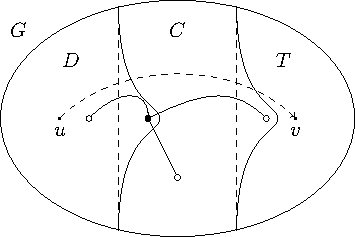
\includegraphics{./img/complexity_intro/GraphVisit.pdf}
    \end{center}
    \caption{Rappresentazione grafica dello schema di algoritmo di visita}
    \label{GraphVisit}
\end{figure}

La complessità è lineare nel numero degli archi. Tutti gli archi devono essere visitati almeno una
volta, se vogliamo fare una visita completa.

Tanti algoritmi di visita possono essere visti come modifiche di questo algoritmo qui andando a
lavorare su come viene gestita l'aggiunta di nuovi nodi a Current. Se si aggiunge in cima
si ha una politica in profondità (LIFO). Nel caso duale si ha una visita in larghezza. Queste sono
fondamentalmente le uniche due visite che hanno senso.

Visita in profondità e larghezza hanno caratteristiche diverse. La visita in profondità non
garantisce di trovare il cammino di lunghezza minima, quella in larghezza invece permette di trovare
sempre il cammino di lunghezza minima che collega il mio nodo di partenza ad un altro nodo del
grafo. La ricerca di un cammino minimo tra due nodi è un'operazione semplice.

È semplice calcolare il cammino più lungo in un grafo? Se lo fosse potremmo controllare la sua
lunghezza. Se questa fosse uguale a $n$ allora avremmo anche un cammino hamiltoniano. La ricerca di
un cammino lungo è quindi equivalente alla ricerca di un cammino hamiltoniano. E quindi è anche un
problema $\NPClass$-completo (lo vedremo più avanti).

In un certo senso il duale di un problema semplice è un problema difficile (cammino minimo vs.
cammino massimo). Non basta una semplice scansione dei cammini per trovare il più lungo, ma bisogna
considerarli tutti. Questo rende più complessa la ricerca.

Cercare cammini brevi è un'operazione facile, cercare cammini lunghi è difficile.

\section{Analisi di problemi}

Quando abbiamo un problema dobbiamo innanzitutto trovare un algoritmo stupido per dare un primo
upper bound alla complessità del problema. Gli algoritmi stupidi in genere fanno ricerche
esaustive. L'algoritmo stupido aiuta a cominciare a comprendere il problema.

Ad esempio, per trovare il cammino più lungo possiamo scansionare tutti i cammini semplici e dire
qual è il più lungo. Che upper bound abbiamo? Supponiamo di avere un grafo completamente connesso.
Possiamo calcolare il numero di cammini con tutte le permutazioni possibili tra $u$ e $v$. Abbiamo
quindi un numero fattoriale di cammini rispetto al numero dei nodi, e di conseguenza rispetto alla
dimensione del grafo. Questa complessità è dell'ordine di $n^{n}$: $n! \sim n^{n}$. 

Un grafo completamente connesso rappresenta un caso particolarmente sfavorevole. Tuttavia anche per
i grafi sparsi abbiamo un numero notevole di cammini. Tipicamente il numero è esponenziale o più
che esponenziale. Ad esempio in un grafo come quello della figura \ref{PathsNumber} abbiamo un
numero di archi che è lineare nell'ordine dei nodi ma abbiamo comunque un numero esponenziale di
cammini tra due nodi.

\begin{figure}[h]
    \begin{center}
        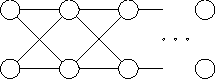
\includegraphics{./img/complexity_intro/ExponentialPathsNumber.pdf}
    \end{center}
    \caption{Esempio di grafo ``semplice'' con un grande numero di cammini possibili}
    \label{PathsNumber}
\end{figure}

La ricerca esaustiva è costosa. In linea di massima potremmo dare lo stesso upper bound per la
ricerca di cammini minimi. In realtà per fortuna con la ricerca breadth-first possiamo visitare i
nodi in ``ordine di distanza''. In questo modo possiamo individuare in maniera semplice i cammini
minimi. È quasi un miracolo in considerazione dello spazio di ricerca delle soluzioni di dimensione
esponenziale che abbiamo. 

Accade spesso che algoritmi polinomiali derivino dal fatto che invece di una ricerca esaustiva
possiamo farne una più mirata, grazie a particolari condizioni e risultati.

L'altro test semplice che si deve sempre fare è: ``data una soluzione esiste un modo semplice per
verificare che una soluzione sia corretta in modo efficace''? È possibile ``certificare'' in maniera
semplice una soluzione?

Il certificato per un cammino massimo non è banale: come facciamo a verificare che sia davvero il
massimo in maniera efficiente? Viceversa è invece banale il certificato per un cammino di lunghezza
$k$. Questo ammmette una verifica semplice, e questo colloca il problema di cercare un cammino di
lunghezza $k$ tra due nodi in un grafo in $\NPClass$, che è una classe piccola di problemi
esponenziali.

Una volta che abbiamo capito che sta in $\NPClass$ possiamo passare a chiederci se sta anche in
$\PClass$ e cominciare la ricerca di un algoritmo efficiente.

\subsection{Colorabilità}

Un altro problema interessante sui grafi è la colorabilità: capire se un dato grafo è colorabile con
$n$ colori. La ``difficoltà'' del problema problema dipende dal valore di $n$. La bicolorabilità di
un grafo è un problema semplice. Non tutti i grafi sono bicolorabili (vedi Figura
\ref{TwoColorableGraphs}). Un grafo può essere bicolorabile in più di un modo, a seconda di quale
colore scegliamo per iniziare la colorazione. Tuttavia questo non è un problema, dato che possiamo
sempre passare da una colorazione all'altra semplicemente complementando i colori.

\begin{figure}[h]
    \begin{center}
        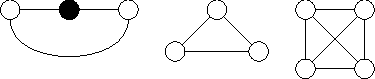
\includegraphics{./img/complexity_intro/2ColorableGraphs.pdf}
    \end{center}
    \caption{Esempi di grafi bicolorabili e di grafi non bicolorabili}
    \label{TwoColorableGraphs}
\end{figure}

Se abbiamo una cricca di dimensione $n$ abbiamo bisogno di almeno $n$ colori per colorarla, se
questa è in effetti colorabile. La colorabilità di un grafo è legata alla densità degli archi del
grafo.

La bicolorabilità è facilmente risolvibile mediante una visita. Il procedimento è a grandi linee
questo:
\begin{itemize}
    \item Ci poniamo la seguente invariante: i nodi già visitati e i nodi nella frontiera sono già
    stati colorati. Coloriamo quando aggiungiamo alla frontiera;
    \item Nella frontiera corrente selezioniamo un nodo;
    \item Andiamo a guardare i nodi connessi al corrente e facciamo la verifica di coerenza:
    \begin{itemize}
        \item Per ogni arco che ci riporta in Done verichiamo che i colori siano diversi, altrimenti
        ci blocchiamo. Questo perché il colore è forzato, se troviamo un'incoerenza non è
        possibile procedere altrimenti;
        \item Facciamo lo stesso controllo in Current.
    \end{itemize}
    \item Per i nodi in Todo li spostiamo in Current, assegnandoli un colore. Quale? Il colore
    complementare del current.
\end{itemize}

Se l'algoritmo arriva a termine senza bloccarsi il grafo è bicolorabile.

\begin{figure}[h]
    \begin{center}
        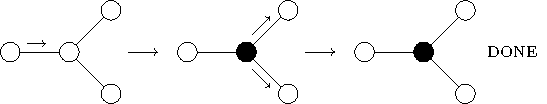
\includegraphics{./img/complexity_intro/2Coloration.pdf}
    \end{center}
    \caption{Esempio di bicolorazione di un grafo}
\end{figure}

Possiamo svolgere questo processo in una sola passata. Come mai? Perché l'assegnazione di colore è
univoca. Questo non è il caso con più di due colori: con tre colori potremmo scegliere tra due
alternative, e dovremmo fare backtracking. Il backtracking può portare (e in genere porta) ad
un'esplosione esponenziale.

Già la 3-colorabilità è un problema $\NPClass$-completo. Perché sta in $\NPClass$? Perché è
facile verficare la correttezza della colorazione, con una semplice visita arbitraria. $\NPClass$ è
una classe ragionevolmente vicina a $\PClass$.

\subsection{Problemi di flusso}

Una classe di problemi tipici sui grafi è quella dei problemi di flusso.

\begin{defn}
    Una rete $N$ è un grafo orientato con una sorgente $s$, un pozzo $t$ e una capacità $c(u,v)$
    associata ad ogni arco.
\end{defn}

\begin{defn}
    Un flusso in $N$ è una funzione $f(u,v)$ che ad ogni arco $(u,v)$ associa un intero positivo
    tale che
    \begin{itemize}
        \item $f(u,v) \leq c(u,v)$;
        \item la somma dei flussi entranti in ogni nodo (esclusi $s$ e $t$) è uguale alla
        somma dei flussi uscenti.
    \end{itemize}
\end{defn}

Il problema del flusso massimo è capire qual è il flusso massimo che la rete supporta, ovvero il
flusso tale che la somma dei flussi uscenti da $s$ (o equivalentemente di quelli entranti in $t$)
sia massima. Ci chiediamo quanto ``fluido'' riusciamo a far passare dalla sorgente al target. Un
upper bound è dato dal minimo tra la somma delle capacità degli archi uscenti dalla sorgente e la
somma di quelli entranti nel target. È un'importante ipotesi che le capacità siano intere.

%Noi vedremo un algoritmo semplice pensato per un caso particolare e una data complessità.
Vediamo un algoritmo semplice per risolvere il problema.

Per risolvere il problema inizialmente cerchiamo dei flussi banali, ovvero dei flussi lineari: la
quantità di fluido si incanala lungo un unico cammino. Quello che cerchiamo quindi è un cammino
qualunque tra sorgente e target. Lungo quel cammino cerchiamo di capire quanto fluido riusciamo a
far passare. Questo è limitato dalla capacità dell'arco di capacità minima nel cammino. Di
conseguenza definiamo un flusso che faccia uscire questa quantità di fluido dalla sorgente e la
faccia entrare nel target lungo il cammino.

Si procede in questo modo finché non ci sono più cammini tra $s$ e $t$, con l'accorgimento di fare
degli ``aggiustamenti'' alla rete legati al fatto che su alcuni archi stiamo già facendo passare del
flusso. Un'operazione è quella di diminuire la capacità di un arco lungo cui stiamo facendo già
passare del fluido, un'altra è quella di diminuire il fluido lungo un arco per farlo passare lungo
un altro.

L'algoritmo è dimostrabilmente corretto; andiamo quindi a discutere la complessità computazionale
dell'algoritmo.

La ricerca di flussi e la somma di flussi sono operazioni lineari nella dimensione del grafo.

Quante iterazioni faremo al massimo? Con ogni operazione diminuiamo almeno di uno il flusso massimo
che passa attraverso la rete. Usando gli upper bound sul flusso massimo dati prima abbiamo un
upper bound alle iterazioni.

Più formalmente procediamo per maggiorazioni. Indichiamo la capacità massima degli archi nel grafo
con $C$. Se supponiamo che tutti gli archi abbiano quella capacità abbiamo un upper bound $nC$ al
flusso massimo. La complessità delle operazioni di ricerca del flusso e applicazione del flusso è
$n^{2}$, quindi abbiamo una complessità dell'ordine $O(n^{3}C)$. È una complessità polinomiale?  No,
$C$ è un numero. In complessità bisogna stare attenti, specie quando abbiamo queste strutture
etichettate. La complessità dovrebbe essere un logaritmo di $C$ se volessimo un algoritmo
polinomiale. In effetti esistono casi patologici che fanno esplodere la complessità per via di $C$.

Data questa considerazione il nostro algoritmo non è polinomiale. Da ricordare è che se la
dimensione dei numeri è logaritmica, la complessità deve essere lineare nella dimensione dei dati.

Possiamo migliorare l'algoritmo? Sì, facendo una ricerca di cammino minimo quando andiamo a cercare
dei flussi. In questo caso la complessità diventa polinomiale. Possiamo risolvere il problema del
flusso massimo in tempo polinomiale.

\section{Problemi decisionali}

Un altro concetto importante è la differenza tra problemi di ottimizzazione e problemi di
decisione. Nel caso del flusso massimo abbiamo un problema di ottimizzazione. Abbiamo dei vincoli e
cerchiamo la soluzione minima (o massima) che soddisfa tali vincoli. In teoria della complessità
siamo interessati a problemi decisionali, ovvero con soluzione booleana Sì/No.

In un certo senso possiamo vedere i problemi di ottimizzazione come dei particolari problemi di
decisione, specie per i problemi di ottimizzazione discreti. Il trucco è, invece di chiederci se
esiste un flusso massimo, ci chiediamo ``esiste un flusso maggiore di $n$?''. È un problema meno
informativo, ma se sappiamo risolvere il problema decisionale possiamo pensare ad un algoritmo
efficiente per risolvere il problema di ottimizzazione. Ad esempio potremmo creare un loop che
esegue il nostro algoritmo per il problema decisionale per valori diversi dell'input finchè non
troviamo il massimo o minimo. Questo tuttavia non è molto astuto come metodo, ne esistono di
migliori.

Di solito risolvendo il problema di ottimizzazione non abbiamo la soluzione in sè, ma un valore
numerico tramite cui possiamo risalire alla soluzione in modo agevole. In altri termini otteniamo la
$x$ invece che la $f(x)$. Ma la $f$ è facilmente calcolabile, di conseguenza questo non è un
problema. Nel caso del problema del flusso massimo di solito la soluzione che otteniamo è il flusso,
non il suo valore. Tuttavia questo è facilmente calcolabile con la somma dei valori del flusso
sugli archi uscenti dalla sorgente, ad esempio.

Restringersi a problemi decisionali non è una decisione problematica, ed è interessante a livello
matematico. Perciò in complessità di solito si fa questa assunzione. Per noi il problema della
cricca sarà ``questo grafo ha una cricca di dimensione $k$?''.

\section{Problemi e linguaggi}

Nel problema decisionale abbiamo delle stringhe che descrivono l'input, in un qualche alfabeto.  Per
alcune stringhe la risposta al problema sarà Sì, per altre No. Il problema ci dà quindi un
linguaggio di stringhe che rappresentano input per cui la soluzione è Sì. La teoria della
complessità si può ridurre al problema di riconoscere stringhe di un linguaggio. L'algoritmo di
decisione del problema può essere visto come un algoritmo di riconoscimento del linguaggio delle
stringhe corrette. Le classi di complessità saranno quindi insiemi di linguaggi riconoscibili da
una macchina di Turing deterministica o meno con una data complessità.  Gli insiemi di linguaggi
sono pensati senza un'architettura specifica in mente.

\section{Riduzioni}

Un'altra problematica importante in Complessità e il problema della riduzione. Lo vediamo guardando
il problema del matching bipartito.

\subsection{Matching bipartito}

\begin{defn}
    Un grafo bipartito è una tripla $B = (U,V,E)$ dove $U$ e $V$ sono insiemi di uguale
    cardinalità e $E \subseteq U \times V$ è un insieme di archi.
\end{defn}

\begin{defn}
    Un matching per un grafo bipartito $B = (U,V,E)$ è un insieme $M \subseteq E$ che associa ad
    ogni elemento in $U$ uno e un solo elemento in $V$.
\end{defn}

Un grafo può essere suddiviso, a livello dei nodi, in due insiemi, tipicamente dalla stessa
cardinalità, i cui elementi non sono collegati. Otteniamo così un grafo bipartito.

Il problema del matching bipartito consiste nello stabilire se per un grafo bipartito esista o meno
un matching.

Non per tutti i grafi bipartiti esiste un accoppiamento, e non è del tutto ovvio come van create le
coppie.

Come lo risolviamo? Un approccio possibile è quello di sfruttare un algoritmo già noto e corretto
per un altro problema simile. Nel nostro caso possiamo sfruttare l'algoritmo per il problema del
flusso massimo. L'idea è che possiamo ridurre il problema del matching bipartito ad un problema di
flusso massimo.

Per fare ciò facciamo la seguente trasformazione al grafo bipartito $B = (U,V,E)$, ottenendo quindi un grafo
$B'$:
\begin{itemize}
    \item aggiungiamo un nodo $s$ ed un nodo $t$;
    \item aggiungiamo un arco da $s$ ad ogni nodo in $U$;
    \item aggiungiamo un arco a $t$ da ogni nodo in $V$;
    \item assegnamo ad ogni arco una capacità unitaria.
\end{itemize}

A questo punto per $B$ esiste un matching bipartito se e solo se $B'$ ammette un flusso massimo di
entità $n = |U| = |V|$, ovvero tale che il flusso totale uscente da $s$ sia uguale a $n$.

Questo è un tipico esempio di riduzione. Abbiamo un problema, il matching bipartito, e lo riduciamo
ad un altro problema, che sappiamo già risolvere. Utilizziamo il problema del flusso massimo per risolvere
il nuovo problema. Che operazione facciamo per fare ciò? L'unica cosa che facciamo è trasformare
i dati di input in una rete di flusso. Dopodiché li diamo in input all'algoritmo per il flusso
massimo. In base alla risposta del primo abbiamo automaticamente la risposta del secondo.

\begin{figure}[h]
    \begin{center}
        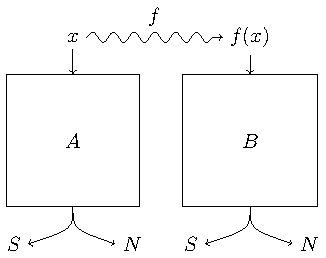
\includegraphics{./img/complexity_intro/Reducibility.pdf}
    \end{center}
    \caption{Schema di riduzione di un problema $A$ in un problema $B$}
\end{figure}

La tentazione di solito è quella di cambiare un algoritmo per adattarlo ad un nuovo problema. In
questo caso non facciamo quello; noi prendiamo i dati di input e li trasformiamo in modo che
l'algoritmo iniziale lo possa accettare. L'algoritmo rimane lo stesso, quello che viene adattato è
l'input. Questo significa fare una riduzione.

Avremo però qui dei vincoli in più rispetto alla riduzione della teoria della calcolabilità. Ad
esempio avremo vincoli sul costo computazionale di $f$. Qui è in un certo senso più intuitivo
rispetto alla teoria della calcolabilità, dato che facciamo trasformazioni da strutture dati a
strutture dati (che per noi sono sempre stringhe), mentre in teoria della calcolabilità si
trasformano numeri in numeri.

Esiste un'altra nozione di riducibilità, la Turing riducibilità. Immaginiamo un oracolo che risolve
$B$ e che possiamo interrogare quante volte vogliamo. Possiamo ora risolvere un dato problema $A$?
In questo caso avremmo che $A$ è Turing-riducibile a $B$.

Per quanto riguarda il concetto di riduzione possiamo pensare ad un problema $A$ e ad un problema
$B$ come linguaggi. Con una riduzione da $A$ a $B$ abbiamo che $x \in A \iff f(x) \in B$. Questa è una
nozione di riducibilità, ce ne sono altre più potenti.

\subsection{Riducibilità e classi di complessità}

La riducibilità è interessante ai fini della complessità. Supponiamo di avere una classe di
complessità $\CClass$ e supponiamo che $B \in \CClass$. Se riusciamo a ridurre $A$ a $B$ vorremmo
poter concludere che anche $A \in \CClass$.

Per fare ciò è importante prendere una nozione di riducibilità abbastanza fine per le classi a
cui siamo interessanti. Una riduzione troppo forte, come la Turing-riducibilità, potrebbe dare
problemi.

Ad esempio pensiamo di poter complementare la risposta di un oracolo. In questo caso potremmo
ridurre ogni linguaggio al suo complementare, che non è sempre quello che vogliamo. Potremmo non
essere in grado di osservare differenze tra classi con una nozione così forte, mentre con una più
debole (o fine) possiamo osservare certe differenze. Con riduzioni forti le classi in un certo senso
collassano. Questo è interessante se vogliamo studiare classi di complessità (o linguaggi) che non
sono chiuse per complementazione.

\begin{figure}[h]
    \begin{center}
        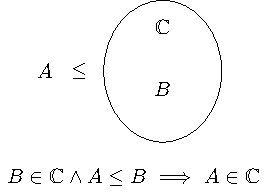
\includegraphics{./img/complexity_intro/ReducibilityNotion.pdf}
    \end{center}
    \caption{Chiusura di classi di complessità in base alla nozione di riducibilità}
    \label{ReducibilityNotion}
\end{figure}

Tutte le classi non deterministiche non sono chiuse per complementazione (come non lo erano insiemi
r.e.). Ad esempio i complementari di linguaggi in $\NPClass$ stanno in $\CONPClass$. In questo caso
non ha senso usare una nozione troppo forte di riducibilità.

Concludere l'appartenenza di $A$ in una classe $\CClass$ in base alla sua riducibilità ad un
problema $B$ in $\CClass$ non è immediato e dipende dalla nozione di riducibilità. In particolare
andrà dimostrato.

\subsection{Complessità di $f$}

La nozione di base di riducibilità l'abbiamo data, ma non basta. Si pongono dei limiti su $f$: si
richiede che $f$ abbia complessità polinomiale in tempo. Questo perché vogliamo che valga la
proprietà di chiusura della figura \ref{ReducibilityNotion}. Infatti se risolviamo $B$ in tempo
polinomiale e $f$ opera una trasformazione anch'essa polinomiale in tempo, componendo i due
algoritmi avremmo un nuovo algoritmo polinomiale in tempo per risolvere $A$.

Richiedere che $f$ sia addirittura lineare sarebbe più fine di quanto ci interessa: sarebbero troppi
pochi i problemi riducibili ad un dato problema. Un vincolo polinomiale sembra essere abbastanza
ragionevole.  Ammettere funzioni di riduzione esponenziali permetterebbere di ridurre
fondamentalmente qualsiasi problema a qualsiasi altro.

Problemi che appartengono apparentemente a domini completamente diversi possono essere agevolmente
ridotti l'uno all'altro. Ad esempio $\SAT$ è riducibilie alla copertura di vertici di un grafo. La
soddisfacibilità è stato il primo problema ad essere stato dimostrato essere $\NPClass$-completo. Se
abbiamo un problema $A$ che è $\NPClass$-completo e abbiamo $B$ tale che $A \leq B$ diremo che $B$
è $\NPClass$-hard.

Le riduzioni aiutano a vedere i problemi in un modo diverso dal solito.

Vediamo alcuni esempi di riduzioni polinomiali tra problemi.

\subsection{Colorabilità}

Vediamo ora che la $n$-colorabilità e riducibile alla $n+1$-colorabilità: $n\textsc{-color} \leq
n+1\textsc{-color}$.

Cosa prende in input $n$\textsc{-color}? Un grafo e dice se è $n$ colorabile. Fissiamo $n$ a 3 e dimostriamo
che $3\textsc{-color} \leq 4\textsc{-color}$.

Possiamo fare la riduzione con la nozione di riducibilità che abbiamo visto prima?

Bisogna fare attenzione a ``non dare per ovvia la soluzione''. Ad esempio è pressocchè sempre
sbagliato pensare che la funzione di riduzione sia l'identità, dato che l'identità solitamente
permette solo di ridurre un linguaggio a se stesso. In questo caso avremmo un verso ma non avremmo
l'altro: un grafo 3-colorabile è sicuramente 4-colorabile ma non vale il viceversa, il che è
importante per la riduzione.

Cosa dobbiamo fare? Dobbiamo prendere il grafo $G$ in input per 3\textsc{-color} e trasformarlo in
un grafo $G'$ che soddisfi la condizione di riduzione. Prendiamo $G$ e aggiungiamo un nodo che
colleghiamo a tutti i nodi di $G$. Per poter colorare questo nodo abbiamo bisogno di un colore nuovo
non in $G$.  Se $G$ è 3-colorabile allora $G'$ è 4-colorabile. Viceversa se $G'$ è 4-colorabile
il colore usato dal nodo aggiunto deve essere diverso da quello dei nodi del sottografo che
corrisponde a $G$, che quindi risulta 3-colorabile.

\begin{figure}[h]
    \begin{center}
        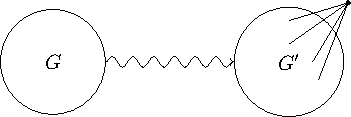
\includegraphics{./img/complexity_intro/3COL4COL.pdf}
    \end{center}
    \caption{Riduzione del problema della $n$-colorabilità alla $n+1$-colorabilità}
\end{figure}

\subsection{Cricca e insieme indipendente}

Vediamo un altro esempio. Proviamo a ridurre il problema dell'insieme indipendente al problema della
cricca: $\textsc{is} \leq \textsc{cricca}$.

L'input di \textsc{is} è una coppia $(G,k)$ e ci chiediamo se esista un insieme indipendente di
dimensione $k$. L'input di CRICCA è una coppia $(G,k)$ e chi chiediamo se esista una cricca di
dimensione $k$.

La trasformazione è semplice: complementiamo il grafo. Dove c'era un insieme indipendente di nodi
avremo tutti i collegamenti possibili tra di essi, e quindi una cricca.

\section{Ricerca vs. Verifica}

%// TODO
%Slide 40

Un conto è cercare una soluzione, un conto è verificare la correttezza di una soluzione.

Di nuovo, quando incontriamo un problema bisogna pensare innanzitutto all'algoritmo stupido di
ricerca esaustiva.

%La complessità dell'algoritmo stupido per l'insieme indipendente è polinomiale per $k$ fissato. Se $k$
%però fa parte del'input questo non è più necessariamente vero. Con $k \in O(n)$ abbiamo un
%algoritmo esponenziale.

Non sempre il certificato è una soluzione al problema. È un'informazione in più che ci viene data e
che ci permette di verificare in modo agevole la correttezza di una data soluzione. Non per tutti i
problemi è possibile effettuare la verifica in tempo polinomiale (e.g. torri di Hanoi).

$\NPClass$ è una classe interessante perché contiene problemi facilmente certificabili.

\section{Relazioni tra alcune classi di complessità}

Cosa significa $A \in \NPClass$? Significa che $\exists B \exists p, B \in \PClass \land p\textit{ polinomio}$
tale che
\begin{equation*}
    x \in A \iff \exists c_{x}, |c_{x}| \leq p(x) \land \pair{x}{c_{x}} \in B
\end{equation*}

La seconda parte dello statement ci dice che possiamo verificare che $c_{x}$ è un buon certificato per
$x$ in tempo polinomiale. La prima parte dice che il certificato deve avere dimensione polinomiale.

Il linguaggio delle coppie $\pair{x}{c_{x}}$ deve far parte di $B$ sse $x \in A$. 

C'è una differenza tra parlare di linguaggi e di macchine. Un linguaggio appartiene ad una certa
classe se esiste una MdT che lo riconosce secondo le condizioni della classe, ma non è la macchina
a far parte della classe. Le classi di complessità comprendono linguaggi, non macchine.

Per tanti problemi possiamo certificare la correttezza con un certificato, per altri no. Ad esempio
per la soddisfacibilità si può fare, per la tautologicità no. Il problema è la dimensione del
certificato.

Per tutti i problemi abbiamo un algoritmo generate and test, il problema sta nella ricerca che è
costosa.

%// TODO
%Slide 43

Ci sono alcuni problemi in $\NPClass$ di cui non si è dimostrata la completezza ma di cui se si potesse
dimostrare l'incompletezza avremmo $\PClass \not= \NPClass$. Finora non si è dimostrata l'incompletezza di
nessun problema in $\NPClass$.

%A volte è possibile verificare che una soluzione sia corretta mediante un certificato ma potrebbe
%non essere possibile verificare che una solzuione si scorretta (sempre mediante certificato)

Si congettura la gerarchia di classi di complessità mostrata in figura \ref{ConjecturedHierarchy}.

\begin{figure}[h]
    \begin{center}
        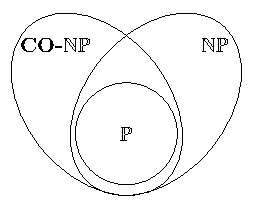
\includegraphics{./img/complexity_intro/NPCONP.pdf}
    \end{center}
    \caption{Gerarchia congetturata di alcune classi di complessità}
    \label{ConjecturedHierarchy}
\end{figure}

Si congettura che $\NPClass$ sia diverso da $\PClass$, e che l'intersezione tra $\CONPClass$ e
$\NPClass$ sia diversa da $\PClass$. Abbiamo che $\COPClass$ è uguale a $\PClass$. Se si dimostra,
come si congettura, che $\COPClass$ sia diverso da $\CONPClass$ allora avremmo anche che $\NPClass$
sarebbe diverso da $\PClass$. Se si dimostra $\PClass = \NPClass$ allora
collasserebbero tutte su $\PClass$. Abbiamo inoltre che ogni problema non banale in $\PClass$ è
$\PClass$-completo. Se si dimostrasse che esiste un problema in $\NPClass$ incompleto avremmo
$\PClass \not= \NPClass$.

Un problema molto studiato è quello dell'isomorfismo tra grafi. Il problema è capire se due grafi
$G,G'$ sono isomorfi, ovvero hanno la stessa struttura topologica. È un problema che ha un sacco di
applicazioni concrete.

Possiamo certificare una soluzione per questo problema? Sì, con il mapping usato. Il numero di mapping
è esponenziale, perciò una ricerca esaustiva non è un granché. Di solito si cerca di pilotare la
ricerca in modo da renderla più veloce, ad esempio sapendo che certi nodi non possono essere
mappati in certi altri in base a certe condizioni.

Si congettura che questo problema, in questa forma, non sia completo. Non se ne è ancora dimostrata
la completezza. C'è un problema simile, che è quello dell'isomorfismo di sottografo. Quello è un
problema completo. Questo perché generalizza il problema della cricca.

Vediamo un problema che sta in $\CONPClass \cap \NPClass$ che si congettura non essere completo
(altrimenti collasserebbe tutto).

Questo problema è la fattorizzazione di un numero intero. La versione decisionale prende $(n,k)$ e
ci chiediamo se $n$ è fattorizzabile con meno di $k$ fattori. Sta in $\NPClass$? Sì. Non è banale
perché fino a poco tempo fa non si sapeva se il test di primalità fosse polinomiale. Ma sappiamo
ora che lo è, quindi la verifica della fattorizzazione è semplice.

Abbiamo un certificato per dire che un numero non è fattorizzabile in meno di $k$ fattori? Sì,
sempre la fattorizzazione. Questo perché la fattorizzazione è unica.

Il certificato va bene per entrambi i casi, basta cambiare il metodo di verifica.

%% tex/deterministic_complexity_classes.tex
%% Copyright 2019 Andrea Berlingieri
%
% This work may be distributed and/or modified under the
% conditions of the LaTeX Project Public License, either version 1.3
% of this license or (at your option) any later version.
% The latest version of this license is in
%   http://www.latex-project.org/lppl.txt
% and version 1.3 or later is part of all distributions of LaTeX
% version 2005/12/01 or later.
%
% This work has the LPPL maintenance status `maintained'.
%
% The Current Maintainer of this work is Andrea Berlingieri.
%
% This work consists of all files listed in manifest.txt
\chapter{Classi deterministiche di complessità}

\section{Macchine di Turing}

La macchina di Turing è un celebre modello di calcolo introdotto in \ref{sec:turingmachine}. Lo
rivediamo qui per comodità in una versione leggermente diversa (multi-tape).

\begin{defn}
    Una Macchina di Turing (multi-tape, deterministica) è una tupla $\tuple{Q, \Gamma, b, \Sigma,
    k, \delta, q_{0}, F}$ dove
    \begin{itemize}
        \item $Q$ è un insieme finito di stati
        \item $\Gamma$ è l'alfabeto finito del nastro
        \item $b$ è il carattere bianco
        \item $\Sigma \subseteq \Gamma \setminus \set{b}$ è l'insieme dei caratteri di input/output
        \item $k \geq 1$ è il numero di nastri
        \item $q_{0} \in Q$ è lo stato iniziale
        \item $F \subseteq Q$ è l'insieme degli stati finali (o di accettazione)
        \item $\delta: Q \setminus F \times \Gamma^{k} \to Q \times \Gamma^{k} \times
        \set{L,R}^{k}$ è la funzione di transizione.
    \end{itemize}
\end{defn}

Intuitivamente abbiamo una serie di nastri con memoria illimitata, divisi in celle di dimensione
fissata. Ogni cella può contenere un carattere di un alfabeto dato, compreso un carattere $b$
(bianco) di inizializzazione. Abbiamo una testina mobile di controllo per ogni nastro ed un automa
di controllo a stati finiti.

Le operazioni fondamentali sono la lettura o scrittura di caratteri individuati dalla testina, lo
spostamento della testina verso destra o verso sinistra, e la modifica dello stato interno
dell'automa.

Per le misure di complessità in genere si tende sempre a prendere come riferimento la macchina di
Turing. Questo perché si tratta di un modello di calcolo semplice in cui sono ben chiari i concetti
di unità di tempo e di unità di spazio, che corrispondono rispettivamente ad una transizione e ad
una cella di memoria.  Ci chiederemo quanti nastri ci permettiamo di usare. Vedremo che questo farà
la differenza.

I nastri sono infiniti, ma in ogni momento si suppone che solo una parte finita del nastro sia stata
scritta. I nastri partono blank, su di essi viene scritto l'input e su di essi si svolge la
computazione.

È la funzione di transizione che governa il comportamento della macchina.

\subsection{Convenzioni di input output}

%Slide 47

Si suppone in genere di avere un nastro di input sul quale possono essere effettuate solo letture e
su cui ci si può muovere in una sola direzione. Non è limitante dato che possiamo sempre copiare il
nastro di input in un nastro di lavoro e fare quello che vogliamo sul nastro copia.

Abbiamo anche un nastro di output, di sola scrittura, la cui testina avanza in una sola direzione.

Si suppone in genere di avere già l'input su nastro prima di cominciare la computazione.  Questa
ipotesi non cambia le considerazioni già fatte sulle complessità sublineari, in genere poco
interessanti. Per convenzione supponiamo che la computazione cominci con la testina sul primo
carattere dell'input, con le altre celle che hanno il carattere blank.

Per convenzione supponiamo che, alla fine della computazione, l'output sia la più lunga stringa di
caratteri dell'alfabeto non blank alla sinistra della testina del nastro di output.

È importante non confondere configurazione iniziale e stato iniziale.

\subsection{Configurazioni}

Una configurazione è una descrizione dello stato della computazione in un dato istante.

Rappresentiamo le configurazioni mediante tuple così fatte:
\begin{equation*}
    q, (\sigma_{1},\tau_{1}),\dotsc,(\sigma_{k},\tau_{k})
\end{equation*}
dove $q$ è lo stato dell'automa e $\sigma_{i}$ e $\tau_{i}$ sono due stringhe di caratteri che
descrivono la porzione non (definitivamente) bianca del nastro $i$ alla sinistra e alla destra della
relativa testina. Il carattere in lettura è il primo carattere di $\tau_{i}$.

La computazione avviene per passi discreti: una transizione tra due configurazioni è una relazione
$\vdash$ governata dalla funzione di transizione:
\begin{equation*}
    (q,(\sigma_{1}b_{1},a_{1}\tau_{1}),\dotsc,(\sigma_{k}b_{k},a_{k}\tau_{k})) \vdash
    (q',(\sigma_{1}\beta_{1},\alpha_{1}\tau_{1}),\dotsc,(\sigma_{k}\beta_{k},\alpha_{k}\tau_{k}))
\end{equation*}
se
\begin{itemize}
    \item $\delta(q,a_{1},\dotsc,a_{k}) = (q',a_{1}',\dotsc,a_{k}',D_{1},\dotsc,D_{k})$
    \item se $D_{i} = R$, allora $\beta_{i} = b_{i}a_{i}'$ e $\alpha_{i} = \varepsilon$
    \item se $D_{i} = L$, allora $\beta_{i} = \varepsilon$ e $\alpha_{i} = b_{i}a_{i}'$
\end{itemize}

La relazione $\vdash^{*}$ denota la chiusura transitiva e riflessiva della relazione $\vdash$.

\begin{defn}
    Una funzione $f: \Sigma^{*} \to \Sigma^{*}$ è calcolata da una macchina di Turing $M$ se per
    ogni $\alpha$ esiste $q_{f} \in F$ tale che
    \begin{equation*}
        q_{0}, (\varepsilon,\alpha),\dotsc,(\varepsilon,\varepsilon) \vdash^{*} q_{f},
        (\gamma_{1},\tau_{1}),\dotsc,(\gamma_{k},\tau_{k})
    \end{equation*}
    e $f(\alpha)$ è il più lungo prefisso di $\gamma_{k}$ appartenente a $\Sigma^{*}$
\end{defn}

Detto in altri termini una computazione parte dallo stato iniziale, con i nastri vuoti, con l'input
sul nastro di input e procede per configurazioni successive, fino ad arrivare ad una configurazione
finale (se la funzione calcolata è definita per il dato input).

\begin{equation*}
    \overequalto{c_{0}}{\varepsilon,q_{0},x} \to c_{1} \to c_{2} \to \cdots \to c_{F}
\end{equation*}

Dato che in complessità noi consideriamo problemi decisionali di solito l'output non è
interessante di per sè. Potremmo avere due stati interessanti, uno di accettazione e uno di
rifiuto.

Nel modello deterministico l'evoluzione della macchina è completamente determinata e univoca per la
macchina considerata dato lo stato iniziale. Lo schema è lineare. La macchina non deterministica
invece non ha una sola mossa disponibile, ne ha un set. Ci possono essere più scelte riguardo alla
mossa successiva.

Lo schema corrispondente smette di essere una sequenza e diventa un grafo, come si puo notare in
figura \ref{img:nondetcomp}.

\begin{figure}[h]
    \begin{center}
        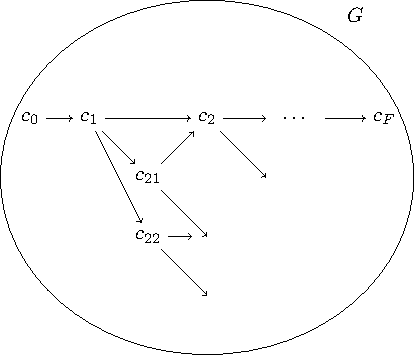
\includegraphics{./img/deterministic_complexity_classes/NonDetComputation.pdf}
        \caption{Schema di una computazione non deterministica}
        \label{img:nondetcomp}
    \end{center}
\end{figure}

La computazione della macchina non deterministica è un grafo con milioni di nodi. Inoltre questi nodi
sono ``grossi'', un sacco di informazione è codificata in ogni nodo. Questo è un esempio vero di
grafo ``grosso'' (Internet a confronto è un grafo piccolo).

Questo è fondamentale per quanto riguarda la simulazione deterministica della macchina non
deterministica. In sostanza questa si riduce alla visita di tutti i cammini del grafo della
computazione della macchina non deterministica.

Il problema è che dobbiamo visitare tutti i cammini del grafo. Solitamente non basta una visita
semplice. Abbiamo il problema di come svolgere questo processo. Lo rivedremo più avanti.

\section{Classi di complessità}

Prima di vedere le classi di complessità definiamo alcune ``grandezze'': $\textit{time}_{M}$,
$\textit{space}_{M}$, $t_{M}$, $s_{M}$.

\begin{defn}
    Sia $M$ una Macchina di Turing.
    \begin{itemize}
        \item $\textit{time}_{M}(x)$ è il tempo di esecuzione di $M$ su input $x$: il numero di
        passi richiesti per la computazione
        \item $\textit{space}_{M}(x)$ è il numero massimo di celle visitate da una qualche testina
        durante la computazione (per macchine a più nastri si considerano solo i nastri di lavoro)
        \item $t_{M}(n) := \max\set{\textit{time}_{M}(x) \mid |x| = n}$
        \item $s_{M}(n) := \max\set{\textit{space}_{M}(x) \mid |x| = n}$
    \end{itemize}
\end{defn}

Se in una computazione abbiamo una configurazione $\tuple{\beta, q, \alpha}$ su qualche nastro dove
la lunghezza di $\beta$ e quella di $\alpha$ sono massime, lo spazio consumato è uguale alla somma tra la
lunghezza di $\beta$ e quella di $\alpha$.

Le prime due grandezze misurano la complessità in funzione dell'input. Tuttavia noi vogliamo
calcolare la complessità in funzione della dimensione dell'input. Definiamo quindi le altre due
grandezze. $t_{M}$ rappresenta il caso pessimo di complessità in tempo per stringhe di lunghezza
$n$. $s_{M}$ è un analogo per lo spazio.

\begin{defn}
    Sia $f:\Nat \to \Nat$. Definiamo le seguenti classi di complessità:
    \begin{itemize}
        \item $\DTIME(f) := \set{\Lang \subseteq \Sigma^{*} \mid \exists M, \Lang = \Lang_{M} \land
        t_{M} \in O(f)}$
        \item $\DSPACE(f) := \set{\Lang \subseteq \Sigma^{*} \mid \exists M, \Lang = \Lang_{M} \land
        s_{M} \in O(f)}$
    \end{itemize}
\end{defn}

La $D$ in queste due classi sta per \textbf{determinstic}.

Le classi di complessità sono classi definite in termini di funzioni. La funzione di input dà un
ordine di grandezza, non una misura precisa. In altre parole siamo interessati ad $O(f)$.

\textbf{Nota bene:} le classi \textbf{non rappresentano tempi o spazi}. Rappresentano classi di
problemi, o, più formalmente, insiemi di linguaggi.

$\DTIME(f)$ rappresenta l'insieme di linguaggi che sono accettabili da una macchina di Turing in un
tempo $O(f)$.

$f$ è una funzione della dimensione dell'input. $\DTIME(n^{2})$ è l'insieme dei linguaggi che sono
riconosciuti da una MdT in tempo quadratico.

\section{Relazione tra spazio e tempo}

Il teorema che vediamo ora è molto importante. È analogo, a livello di importanza, al problema
della terminazione della teoria della calcolabilità. Ci dice qualcosa sulla relazione tra
complessità in tempo e complessità in spazio.

Sapendo che un certo linguaggio ha una certa complessità in tempo possiamo dire qualcosa sulla sua
complessità in spazio, e viceversa?

Partiamo dalla parte più facile. Supponiamo di avere la complessità in tempo di un algoritmo.

Che motivazioni abbiamo per voler sapere la complessità in tempo? Una è sicuramente che il tempo è
una risorsa critica. Inoltre è una misura più fine di quella di spazio, ci dà un upper bound a
quest'ultimo. Questo perché se vogliamo aumentare l'occupazione di spazio, con la MdT, dobbiamo
scrivere nuove celle. Sporcare una nuova cella richiede almeno un'unità di tempo. La complessità in
tempo dà un upper bound stretto alla complessità in spazio.

Questo è importante, ed è anche una delle ragioni per cui il tempo è più interessante dello
spazio.

Questo discorso vale a meno di costanti, dato che definiamo noi l'unità di tempo e spazio. Ma una
volta definite queste il ragionamento resta immutato.

Abbiamo quindi che $\DTIME(f) \subseteq \DSPACE(f)$. A prima vista sembrerebbe un'inversione. In
realtà se ci pensa se abbiamo un upper bound alla complessità in tempo richiesta per risolvere un
problema abbiamo che lo stesso upper bound si applica per la complessità in spazio, e quindi i
linguaggi di $\DTIME(f)$ fanno sicuramente parte di $\DSPACE(f)$.

\begin{thm}
    Sia $f: \Nat \to \Nat$. Allora $\DTIME(f) \subseteq \DSPACE(f)$.
\end{thm}
\begin{proof}
    Supponiamo che $\Lang \in \DTIME(f)$. Abbiamo quindi che $\exists M, \Lang = \Lang_{M} \land
    t_{M} \in O(f)$. Ma se $t_{M} \in O(f)$ allora anche $s_{M} \in O(f)$. Questo perché il tempo
    è un upper bound allo spazio. Ma quindi $\Lang \in \DSPACE(f)$.
\end{proof}

Per dimostrare il teorema abbiamo svolto la nostra analisi sulla stessa macchina. Questo non è
richiesto per la dimostrazione, dato che potremmo immaginare di svolgere la dimostrazione con
un'altra macchina per la parte della complessità in spazio. In questo caso non è stato necessario,
il teorema è puntuale sulla macchina. Se una certa macchina ha una certa complessità in tempo ha la
stessa complessità, al più, in spazio.

Si può occupare anche meno spazio, il tempo fa da upper bound.

Questa era la parte facile, ragioniamo ora sul viceversa. Data la complessità in spazio possiamo
dire qualcosa sulla complessità in tempo?

Supponiamo ad esempio che una certa macchina di Turing lavori in spazio costante. Quando misuriamo
la complessità in spazio in genere abbiamo macchine multinastro. Di solito non consideriamo lo
spazio del nastro di input. Noi consideriamo solo lo spazio aggiuntivo di cui la macchina ha bisogno
per svolgere la computazione.

In questo ha caso ha senso parlare di complessità sublineari, dato che magari non abbiamo bisogno
di uno spazio aggiuntivo della stessa dimensione dell'input. In particolare possiamo avere spazio
costante, indipendente dall'input.

Un punto importante è che la complessità la misuriamo sempre al termine della computazione. Se la
computazione non termina la complessità è indefinita, quindi non è un caso interessante quello di
loop infinito. Se la complessità è definita non possiamo divergere.

Siamo in loop se passiamo per due volte sulla stessa configurazione. Ma noi questo non lo
permettiamo. Perciò abbiamo un insieme finito di possibili configurazioni che verranno assunte in
una computazione che giunge a termine.

Proviamo a calcolare il numero possibile di configurazioni immaginando di lavorare con uno spazio
costante. Consideriamo i possibili nastri diversi di lunghezza $L$. Questi sono $|\Sigma|^{L}$.
Moltiplichiamo per $|Q|$, il numero di stati. Infine moltiplichiamo per $L$, dato che la testina
potrebbe essere su qualsiasi cella del nasto. Otteniamo la seguente quantità:
\begin{equation*}
    L \times |Q| \times |\Sigma|^{L}
\end{equation*}

Questo rappresenta un upper bound alla complessità in tempo del problema.

Il numero degli stati è fissato in base alla macchina. L'ordine è dato da $L$. La crescita è
esponenziale. Non è così grave, c'è molto di peggio.

Questa analisi vale in caso di complessità costante. Cambia qualcosa se la complessità in spazio
ha un ordine $O(s(n))$? No, basta che la mia $L$ diventi una $L(s(n))$. Il discorso si applica
invariato. Sappiamo che o la macchina termina entro questo upper bound oppure è in loop.

Anche qui l'analisi è puntuale. Data una macchina e una complessità in spazio possiamo dare una
complessità in tempo sulla stessa macchina, non ne dobbiamo produrre un'altra.

In un certo senso per alcuni programmi non possiamo decidere la terminazione perché non possiamo
neanche decidere la quantità di spazio che verrà richiesto. Si può dimostrare che se è decidibile il
problema di sapere qual è l'occupazione di una certa risorsa sarebbe decidibile il problema di sapere
qualcosa per un altra risorsa. Questo perché tutte le misure di complessità sono correlate. Questa
correlazione può essere pessima a piacere, nel nostro caso era esponenziale.

In questa analisi stiamo dimenticando qualcosa. Sembrerebbe che se abbiamo una complessità in
spazio costante avremmo una complessità in tempo costante, e quindi sublineare. Tuttavia in realtà
noi dobbiamo sapere anche fino a che punto siamo arrivati nell'input. Questo va ad influire sul
numero delle combinazioni. In particolare va aggiunta la lunghezza dell'input alla misura data
prima.
\begin{equation*}
    n\times L \times |Q| \times |\Sigma|^{L}
\end{equation*}

Quindi abbiamo che, se $M \in \DSPACE(f(n))$ allora $\exists c, M \in \DTIME(c^{f(n) + \log(n)})$.
Ricordiamo che $n = c^{\log_{c}(n)}$.

\begin{thm}
    Sia $f: \Nat \to \Nat$. Allora $\DSPACE(f) \subseteq \bigcup_{c \in \Nat}\DTIME(c^{log + f})$.
\end{thm}

Ancora una volta l'esponenziale non è così male. Tutta la teoria della complessità si gioca tra
esponenziale e polinomiale, è un vincolo abbastanza vicino.

\section{Dipendenza dal modello di calcolo}

La macchina di Turing è molto flessibile dato che ci sono tante variabili che possono influire. Ci
chiediamo quanto questo ci influenzi nella nostra analisi.

Se restringiamo l'alfabeto abbiamo bisogno di stati nuovi per ricordare che ruolo ha un simbolo del
nuovo alfabeto rispetto a quello che aveva nel vecchio.

Lo slowdown è lineare. Se passiamo, ad esempio, da ASCII a binario, dovremo fare 8 passi per uno
equivalente. Era di moda tempo fa la ricerca della macchina di Turing universale che minimizzasse la
somma tra grandezza dell'alfabeto e numero di stati.


\subsection{Riduzione dei nastri}

Vediamo qualcosa di più importante, ovvero la riduzione dei nastri.

Immaginiamo di passare da due nastri ad un solo nastro. Perché è problematico lavorare con un
nastro? Immaginiamo di avere una stringa $l$ sul nastro e di volerla copiare più avanti. Con un
nastro solo questa operazione è molto complessa. Dobbiamo leggere i caratteri $x_{0},\dotsc,x_{n}$
uno alla volta, memorizzando il carattere con uno stato interno. Non possiamo memorizzare l'intera
stringa usando uno stato interno perché non abbiamo un upper bound alla lunghezza della stringa.

\begin{figure}[h]
    \begin{center}
        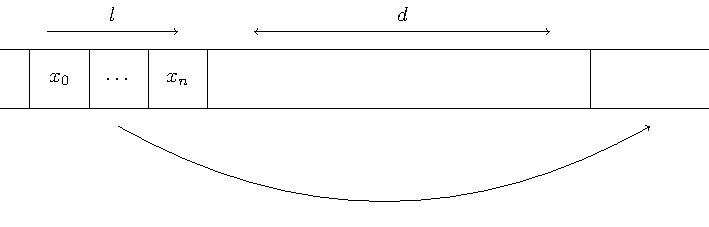
\includegraphics{./img/deterministic_complexity_classes/CopyString.pdf}
        \caption{Copia di una stringa con due nastri}
    \end{center}
\end{figure}

Se la distanza è $d$ sono necessari $d\cdot l$ giri avanti e indietro. Essendo $d$ almeno lineare in $l$
(non consideriamo condizioni di overlap) abbiamo complessità almeno quadratica.

Con due nastri è semplice. Basta copiare la stringa di input su un altro nastro, posizionare la
testina del nastro di input dove vogliamo copiare la stringa e posizionare la testina del secondo
nastro all'inizio della stringa. A questo punto è sufficiente scrivere nel primo nastro il
carattere letto dalla testina sul secondo nastro fino a raggiungere la fine della stringa.

\begin{figure}[h]
    \begin{center}
        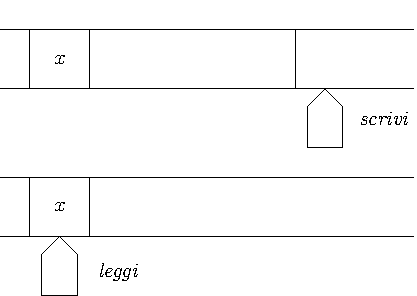
\includegraphics{./img/deterministic_complexity_classes/CopyString2Tapes.pdf}
        \caption{Copia di una stringa con due nastri}
    \end{center}
\end{figure}

Passando da due nastri ad uno abbiamo uno slowdown che può essere quadratico. Questo è pesante. La
complessità computazionale dipende dal modello di calcolo. Nell'ambito delle macchine di Turing
questi slowdown restano però polinomiali.

C'è una sottigliezza da considerare riguardo la macchina a due nastri. Le due testine possono
essere lontane a piacere, e il tempo di trasmissione tra le due può quindi aumentare
arbitrariamente. Non è sempre corretto considerare il costo della trasmissione pari ad 1.

%Slide 50

% TODO maybe move this to the part on the size of the input
%Se pensiamo ad $x$ come una stringa $|x|$ corrisponde alla lunghezza della stringa; per i numeri,
%usando una rappresentazione almeno binaria, abbiamo una dimensione $|x|$ uguale a $\log(x)$.

%Slide 51

% TODO move this somewhere more appropriate
% Lo spazio mi dà un upper bound al tempo, ma questo è molto più lasco.

%Slide 52

% TODO move this somewhere more appropriate
%C'è una dipendenza tra complessità e modello di calcolo che usiamo.

Generalizzando, proviamo a pensare ad una macchina a $k$ nastri e a come simularla con un nastro
solo. Se avessimo un modo efficiente per fare ciò avremmo un modo generale per eseguire un qualsiasi
algoritmo eseguito sulla macchina a $k$ nastri su un solo nastro. La complessità dell'emulatore ci
dà un upper bound alla complessità legato dall'overhead richiesto per la simulazione.

La prima ipotesi che facciamo è la seguente: non poniamo restrizioni sull'alfabeto dei nastri.
Possiamo pensare di avere un alfabeto molto ricco per la macchina ad un nastro. In particolare
possiamo immaginare di avere a disposizione un alfabeto i cui simboli rappresentano l'unione di vari
pezzi dell'alfabeto originale. È in un certo senso analogo all'utilizzo di una parola di memoria a
64 bit per memorizzare due parole di memoria a 32 bit. Come abbiamo visto cambiare l'alfabeto
comporta un overhead lineare.

Facciamo poi un'altra ipotesi: da qualche parte dobbiamo memorizzare la posizione della testina.

Noi immaginiamo di simulare $k$ nastri su un nastro solo utilizzando un alfabeto per il nostro
nastro in cui ogni simbolo rappresenta $k$ nastri e $k$ ``tracce''. I simboli sui nastri simulati
sono simboli dell'alfabeto originale, e sulle ``tracce'' memorizziamo la posizione della testina di
ogni nastro rispetto al nastro simulato. In figura \ref{img:KTapesToOne} è possibile vedere una rappresentazione
grafica di questo processo.

\begin{figure}[h]
    \begin{center}
        % TODO Should probably remake it in Tikz
        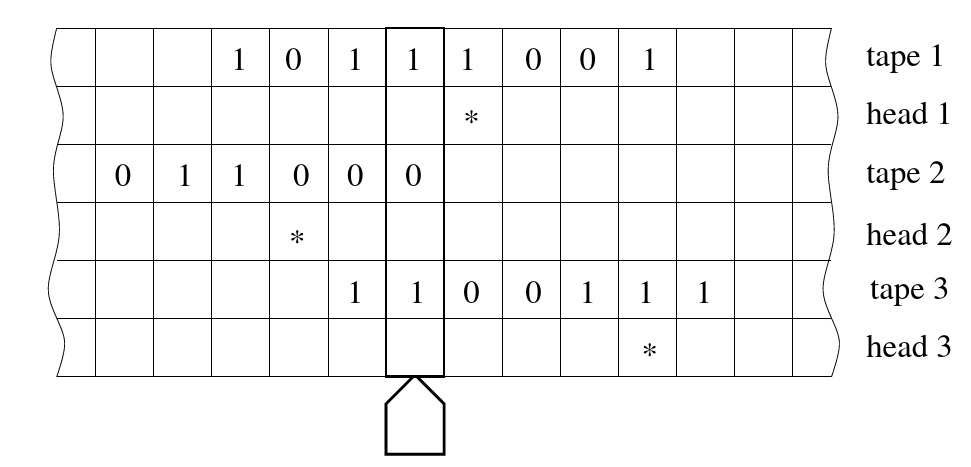
\includegraphics[scale=0.3]{./img/deterministic_complexity_classes/KTapesToOne.png}    
        \caption{Simulazione su una MdT con un nastro di una MdT con più nastri}
        \label{img:KTapesToOne}
    \end{center}
\end{figure}

Se $\Sigma$ è l'alfabeto originale, il nuovo alfabeto è $\Sigma' = (\Sigma \times
\set{*,B})^{k}$.

Proviamo ora a capire quanto ci costa simulare una operazione della macchina a $k$ nastri su questa
macchina.

Ci sono dei piccoli accorgimenti che si possono fare per avere dei miglioramenti dal punto di vista
della complessità in tempo, a dispendio della memoria. Ad esempio potremmo immaginare di
memorizzare dell'informazione ulteriore che ci dia una direzione nella quale dovremmo cercare la
testina, in modo da non dover scansionare l'intero nastro. Tuttavia queste ottimizzazioni non sono
significative a livello di complessità.

Supponiamo di avere due nastri per semplicità. La nostra macchina sarebbe descritta da $n$-uple
così fatte:
\begin{equation*}
    ((a_{1},a_{2}),q,(a_{1}',a_{2}'),q',(M_{1},M_{2}))
\end{equation*}
dove $a_{1},a_{2}$ sono i caratteri in lettura, $M_{1}$ e $M_{2}$ sono le due mosse sulle testine,
$a_{1}'$ e $a_{2}'$ sono i due nuovi caratteri da scrivere e $q$ e $q'$ rappresentano,
rispettivamente, lo stato attuale e il nuovo stato. Questa è una tipica istruzione della macchina a
due nastri.

Simulando questa macchina con un nastro solo abbiamo quindi bisogno di una prima passata del nastro
per capire quali sono i caratteri in lettura e salvarli in uno stato interno. A questo punto
riportiamo la testina all'``inizio'' del nastro e facciamo un'altra passata per scrivere i nuovi
caratteri. Infine facciamo una terza passata per simulare la mossa sui nastri simulati.

Sono quindi necessarie più passate per simulare un'operazione della macchina a più nastri.
Un'operazione che aveva costo 1 ora ha un costo che dipende dall'occupazione di memoria. Possiamo
dare un upper bound alla dimensione del nastro al tempo $t$?  Sì, abbiamo un limite lineare in $t$.
Siamo passati da costo 1 a costo $O(t)$. Inoltre il nostro upper bound non è costante, peggiora col
tempo.

Qual è il costo totale della simulazione? Abbiamo una somma di operazioni di costo lineare. Di
conseguenza avremo un costo totale quadratico.

Abbiamo quindi visto che con una simulazione fatta in questo modo abbiamo un overhead quadratico.
Non abbiamo però dimostrato che passando da $n$ nastri ad un nastro abbiamo necessariamente un
overhead quadratico. Ci potrebbe essere un modo migliore per fare simulazioni che non implica questo
aggravio nella complessità.

Un altro modo in cui potremmo fare la nostra simulazione è quello di utilizzare un alfabeto
$\Sigma' = \Sigma^{k}$, se $\Sigma$ era l'alfabeto di partenza, e immaginare di tenere le testine
tutte allineate e che siano i nastri a muoversi sotto le testine.

Con una simulazione fatta in questo modo non dobbiamo più cercare la testina, i caratteri in
lettura li troviamo subito, le scritture le facciamo immediatamente. Quello che diventa complicato
è fare la mossa. Dobbiamo fare una riscrittura dell'intero nastro per fare questo shift dei nastri
simulati. Questo richiede quantomeno una scansione della memoria occupata.

% TODO c'è un discorso sul fatto che utilizzando 2 testine per la simulazione abbiamo un overhead
% ammortizzato, ma non lo abbiamo visto approfonditamente in classe. Potrebbe essere interessante da
% aggiungere
%
%Passando da $k$ nastri a 2 nastri abbiamo una versione ammortizzata, ma passando ad un nastro solo
%non c'è modo. (Slide 53)

L'overhead di simulare una macchina a $k$ nastri con una macchina ad un nastro solo sembra quindi
essere intrinsicamente quadratico.

% TODO volendo si potrebbe approfondire il discorso su questo linguaggio non riconoscibile in
% o(n^{2}). La dimostrazione è interessante

%Slide 59

A riprova di questo fatto esistono linguaggi che sono riconoscibili in tempo lineare con una
macchina a due nastri, in tempo quadratico con una macchina ad un nastro, ma che non sono
riconoscibili in un tempo che sia un $o(n^{2})$ con una macchina ad un nastro. Un linguaggio con
queste caratteristiche è il seguente:
\begin{equation*}
    \Lang = \set{w\#^{|w|}w \mid w \in \set{0,1}^{*}}
\end{equation*}

La dimostrazione di questo fatto è interessante perché è in generale difficile dimostrare che un
certo problema non si possa risolvere con un algoritmo di complessità migliore di una nota. La
dimostrazione fa inoltre uso della complessità di Kolmogorov.

\subsubsection{Nota sugli slowdown}

Nel calcolare gli slowdown prendiamo un'operazione di costo costante e vediamo quanto costa
eseguirla in un altro modo. In questo modo la complessità dell'altro modo corrisponde allo slowdown
che abbiamo.

Se non abbiamo costo costante dobbiamo fare un'analisi più sofisticata. O prendiamo il caso
pessimo, e così diamo un upper bound. Questo però potrebbe essere troppo esagerato, e sarebbe il
caso di dare un upper bound definito meglio.

\subsection{Random Access Machine}

Quanto dipende la complessità dal modello che utlizziamo? Per rispondere a questa domanda vediamo
un modello di calcolo molto più ``liberale'' della MdT: la Random Access Machine (RAM).

In una RAM abbiamo delle celle di memoria tutte indirizzabili, come se fossero dei registri. Di
queste ne abbiamo una quantità numerabile. Possiamo accedere a queste mediante ``indirizzi'', che
possiamo immaginare per semplicità esssere dei numeri interi. L'ipotesi forte che facciamo è che
ogni registro possa avere dimensione illimitata: in ogni registro possiamo scrivere numeri
arbitrariamente grandi.

Abbiamo, tra i vari registri, il program counter, che è un registro particolare che mantiene la
prossima istruzione da eseguire.

Non è un modello realistico di complessità, proprio per via di questa ipotesi non realistica.

Usiamo le seguenti notazioni:
\begin{itemize}
    \item $r_{i}$ rappresenta il contenuto del registro $i$-esimo. Utilizziamo il registro $r_{0}$
    come accumulatore;
    \item $i_{j}$ rappresenta il $j$-esimo input;
    \item $k$ rappresenta il program counter.
\end{itemize}
Il comportamento della macchina è descritto da programmi composti da una sequenza di istruzioni di
uno dei seguenti tipi:
\begin{itemize}
    \item \textsc{read}, che ha due varianti:
    \begin{itemize}
        \item $\textsc{read }j$, con la seguente semantica: $r_{0} \gets i_{j}$ 
        \item $\textsc{read }\uparrow j$, con la seguente semantica: $r_{0} \gets i_{r_{j}}$ 
    \end{itemize}
    \item \textsc{store}, che ha due varianti:
    \begin{itemize}
        \item $\textsc{store }j$, con la seguente semantica: $r_{j} \gets r_{0}$ 
        \item $\textsc{store }\uparrow j$, con la seguente semantica: $r_{r_{j}} \gets r_{0}$ 
    \end{itemize}
    \item $\textsc{load }x$, con semantica $r_{0} \gets x$
    \item $\textsc{add }x$, con semantica $r_{0} \gets r_{0} + x$
    \item $\textsc{sub }x$, con semantica $r_{0} \gets r_{0} - x$
    \item $\textsc{half}$, con semantica $r_{0} \gets r_{0} / 2$
    \item $\textsc{jump }j$, con semantica $k \gets j$
    \item $\textsc{jpos }j$, con semantica \textbf{if} $r_{0} > 0$ \textbf{then} $k \gets j$
    \item $\textsc{jzero }j$, con semantica \textbf{if} $r_{0} = 0$ \textbf{then} $k \gets j$
    \item $\textsc{halt}$, con semantica $k \gets 0$
\end{itemize}

È molto simile ad un linguaggio Assembler di un tipico calcolatore. Questo è un modello più
vicino alla macchina di Von Neumann rispetto alla MdT. Consideriamo di costo 1 tutte le operazioni
della RAM, indipendentemente dal fatto che lavorino su interi di grandezza arbitraria. Inoltre se
immaginiamo di avere un problema per cui la dimensione dei nostri registri è sufficiente il modello
risulta abbastanza fedele a quello di Von Neumann, e quindi alla realtà.

Questo è un modello abbastanza flessibile e generale, è difficile immaginare di meglio. Questo
giustifica anche l'irrealisticità di questo modello.

Quanto ci costa simulare questa macchina con una MdT? 

Abbiamo delle ipotesi. All'inizio della computazione è caricato in un particolare registro con
l'input, il PC è settato all'inizio del nostro programma e tutte le altre celle sono memorizzate a
vuoto, non contengono informazione.

Il problema principale è come gestiamo la memoria di questa macchina nella MdT. Immaginiamo di
usare un nastro della MdT per la simulazione della memoria. Dobbiamo simulare, registro per
registro, il contenuto dei registri. All'inizio abbiamo solo il registro di input con informazione
interessante.

Non sappiamo in che modo saranno scritti i registri della macchina. Ad esempio non possiamo supporre
che avremo accessi sequenziali (prima il primo registro, poi il secondo, ecc.). Un modo semplice per
simulare la memoria è descrivere ogni registro con due campi: il nome (il numero) e il valore. Ogni
registro corrisponde ad una coppia nome-valore.

\begin{figure}[h]
    \begin{center}
        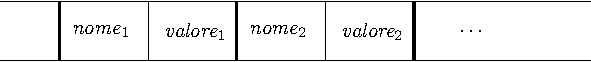
\includegraphics{./img/deterministic_complexity_classes/RAMsimulation.pdf}
        \caption{Simulazione dei regisri di una RAM in una MdT}
    \end{center}
\end{figure}

In generale non possiamo dare un upper bound né al numero dei registri né alla dimensione di
questi. Potremmo avere un numero arbitrario di registri occupati con valori arbitrariamente grandi.

Sul nastro della memoria memorizziamo le coppie in maniera sequenziale.

Immaginiamo di voler simulare un'operazione, ad esempio la somma. Solitamente si immagina il
registro $r_{0}$ come l'accumulatore utilizzato per le operazioni aritmetiche.

Immaginiamo di sommare, ad esempio, al registro $r_{0}$ il valore del registro $r_{25}$. Dovremo
fare una ricerca in memoria del registro $r_{25}$, leggere il valore e sommarlo al contenuto del
registro $r_{0}$. Non abbiamo problemi di dimensione dell'accumulatore se ad esso dedichiamo un
intero nastro.

Non abbiamo limiti sul numero dei nastri, purché sia finito. Non possiamo immaginare un nastro per
registro.

Immaginiamo di voler simulare una memorizzazione, magari del risultato della somma. Dobbiamo quindi
scrivere un nuovo valore al posto del valore del registro $r_{0}$. Dovremmo quindi fare delle
operazioni ulteroiri per simulare la memorizzazione, ad esempio uno shift delle coppie nome-valore
verso destra per fare spazio.

Quello che facciamo è una cosa brutale: cancelliamo il registro (nome-valore) e lo riscriviamo in
fondo. Ha lo stesso costo dello shift, ovvero quello di una scansione della memoria.

\begin{figure}[h]
    \begin{center}
        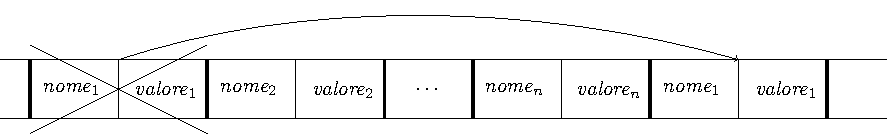
\includegraphics[scale=0.75]{./img/deterministic_complexity_classes/RAMstore.pdf}
        \caption{Simulazione di una memorizzazione in una MdT}
    \end{center}
\end{figure}

Con questo approccio abbiamo problemi di frammentazione e un'occupazione di memoria maggiore
rispetto a quella che avremmo con lo shift, ma in termini di complessità questo non fa alcuna
differenza.

Cosa possiamo dire sulla dimensione della memoria al tempo $t$ della macchina simulata? Ci chiediamo
quanti registri possiamo avere e quanto questi possono essere grandi.

Il numero di registri referenziati è limitato da $O(t)$. Quant'è l'occupazione massima di questi
registri? Sempre $O(t)$. Perché? Abbiamo una sola operazione che aumenta i valori dei registri, e
quindi l'occupazione di memoria: la somma. Abbiamo che la somma di due numeri di dimensione $n$ può
avere al più dimensione $n+1$. Di conseguenza, al tempo $t$, abbiamo una occupazione al più
quadratica della memoria della macchina simulata.

Simulare una operazione della RAM ci costa quindi $O(t^{2})$. Il costo complessivo della somma sarà
la somma dei $t^{2}$ per $t$ che va da 1 a $t_{\textit{fin}}$. Abbiamo quindi un costo totale
$O(t^{3})$.

Simulare una RAM con una MdT può portare ad uno slowdown cubico. Potrebbe andare meglio, ma nel
caso pessimo abbiamo questa complessità. Questa inoltre potrebbe peggiorare se facessimo la
simulazione con un solo nastro.

Possiamo vedere questo risultato in maniera positiva o negativa. Da un certo punto di vista questo
slowdown è gravoso. Dall'altro questo slowdown è comunque polinomiale. In ogni caso un algoritmo
che su RAM aveva complessità polinomiale se simulato con una MdT continuerà ad avere una
complessità polinomiale.

Questo è vero per un modello di calcolo molto liberale. Di conseguenza la complessità
computazionale di un algoritmo dipende dal modello di calcolo, ma se un modello è ``ragionevole''
la complessità dell'algoritmo rimarrà polinomiale anche su questo. La classe polinomiale dei
problemi è quindi una classe relativamente stabile rispetto al modello di calcolo con cui la
studiamo.

Questo è vero entro i limiti di ragionevolezza. Cosa intendiamo? Supponiamo di avere come primitiva
anche l'operazione di moltiplicazione. Quello che succede è che nella simulazione l'occupazione di
memoria esplode: diventa esponenziale. Questo perché con la moltiplicazione l'occupazione di
memoria può crescere di $n$ con un'operazione, dato che il prodotto di numeri di dimensione $n$ ha
può avere dimensione $2n$. Avremmo un overhead esponenziale.

È quindi importante che il modello che utilizziamo abbia un minimo di ragionevolezza. Non ha senso
contare 1 il costo dell'operazione di moltiplicazione. In un certo senso è già strano che
l'addizione abbia costo 1, ma nella RAM lo ammettiamo, e questo si rivela non causare problemi.

Abbiamo quindi due conclusioni importanti:
\begin{itemize}
    \item la complessità computazionale dipende dal modello di calcolo;
    \item se usiamo modelli di calcolo ragionevoli la complessità computazionale su di essi non
    differisce più che polinomialmente.
\end{itemize}

C'è chi parla di generalizzazione della tesi di Church, dove alla calcolabilità corrisponde la
complessità polinomiale e ai modelli Turing completi corrispondono modelli di calcolo ragionevoli.
Tuttavia questo dipende troppo dalle assunzioni che facciamo sul modello di calcolo, e quindi non ha
la generalità e lo spessore della tesi di Church.

%% tex/timespacehierarchies.tex
%% Copyright 2019 Andrea Berlingieri
%
% This work may be distributed and/or modified under the
% conditions of the LaTeX Project Public License, either version 1.3
% of this license or (at your option) any later version.
% The latest version of this license is in
%   http://www.latex-project.org/lppl.txt
% and version 1.3 or later is part of all distributions of LaTeX
% version 2005/12/01 or later.
%
% This work has the LPPL maintenance status `maintained'.
%
% The Current Maintainer of this work is Andrea Berlingieri.
%
% This work consists of all files listed in manifest.txt
\chapter{Gerarchie in spazio e tempo}

%Slide 73

\section{I teoremi della gerarchia}

I teoremi che seguono sono tra i piu' importanti della teoria della calcolabilita'. Riflettono
l'idea intuitiva che disponendo di una quantita' maggiore di risorse e' effettivamente possibile
affrontare problemi piu' complessi.

Consideriamo $\DTIME(n^{2})$, ovvero la classe dei linguaggi riconoscibili in tempo quadratico e
$\DTIME(n^{3})$. Qual'e' la relazione di inclusione tra queste due classi? Abbiamo sicuramente che
$\DTIME(n^{2}) \subseteq \DTIME(n^{3})$.

In generale abbiamo che, se $f,f'$ sono funzioni da $\Nat$ a $\Nat$:
\begin{equation*}
    O(f) \subseteq O(f') \implies \DTIME(f) \subseteq \DTIME(f')
\end{equation*}
Vale lo stesso per lo spazio. Ricordiamo che $O(f) \subseteq O(f') \iff f \in O(f')$.

Ci chiediamo ora, questa inclusione e' stretta? E sotto che ipotesi possiamo affermare cio'?
Esistono, ad esempio, dei linguaggi riconoscibili in tempo $O(n^{3})$ ma non in tempo $O(n^{2})$? E
analogamente per lo spazio?

La risposta e', in un certo senso, positiva, sia per tempo che spazio. Vale piu' per lo spazio che
per il tempo, poiche' lo spazio e' piu' ``grezzo'' del tempo come misura. La separazione in classi
risulta piu' difficile con una misura fine come quella del tempo.

\subsection{Il teorema della gerarchia in spazio}

Vediamo innanzitutto come formalizzare il teorema ponendo la nostra attenzione sullo spazio.  Stiamo
facendo il confronto tra $\DSPACE(n^{2})$ e $\DSPACE(n^{3})$. Quello che vogliamo concludere e' che
dato che $n^{3} \notin o(n^{2})$, allora $\DSPACE(n^{3}) \not\subseteq \DSPACE(n^{2})$. Da cui si
ottiene, data l'inclusione precedente, $\DSPACE(n^{2}) \subset \DSPACE(n^{3})$.

\begin{thm}
    Siano $f,f':\Nat \to \Nat$. Si ha che:
    \begin{equation*}
        f \in O(f') \implies \DSPACE(f) \subset \DSPACE(f')
    \end{equation*}
\end{thm}

Per dimostrare il teorema, dando per ovvia l'inclusione non stretta, ci e' sufficiente dimostrare
che:
\begin{equation*}
    f \notin O(f') \implies \DSPACE(f) \not\subseteq \DSPACE(f')
\end{equation*}

Il teorema in questa forma e' dimostrabile. Esiste tuttavia una forma piu' debole ma piu' intuitiva:
\begin{equation*}
    f' \in o(f) \implies \exists \Lang, \Lang \in \DSPACE(f) \land \Lang \notin \DSPACE(f')
\end{equation*}
Abbiamo rafforzato la premessa dell'implicazione e quindi indebolito il teorema. Ricordiamo che $f'
\in o(f) \implies f \notin O(f')$.

E' uno dei pochi teoremi della teoria della complessita' che ci permettono di separare nettamente
classi di complessita'. Questo e' in contrasto con le tante inclusioni congetturate che non
riusciamo a dimostrare, la piu' famosa delle quali e' la questione $\PClass$  vs $\NPClass$.

\begin{proof}
    Questo teorema e' sicuramente intuitivo nell'enunciato ma non e' ovvio nella dimostrazione.

    Per dimostrare il teorema dobbiamo, sotto l'ipotesi $f' \in o(f)$, definire il nostro linguaggio
    $\Lang$ e poi dimostrare le proprieta' attese per $\Lang$.

    %Ce ne sono diverse di dimostrazioni di questo teorema (sul Sipser ce ne e' una diversa). La
    %dimostrazione non e' banale, va studiata e capita. E' utile farsi guidare dall'enunciato.

    La tecnica tipica che si usa quando si vuole creare un elemento che non faccia parte di una
    certa classe e' la diagonalizzazione. In questo caso definiamo il nostro $\Lang$ per
    diagonalizzazione in modo che non sia riconoscibile in spazio $O(f')$.

    Vediamo prima una versione sbagliata del linguaggio, per poi passare a quella corretta. Questo
    passaggio ci portera' a capire una cosa importante della complessita'.

    Usiamo la notazione $\code{M}$ per denotare il codice della MdT $M$.

    Definiamo $\Lang$ come:
    \begin{equation*}
        \Lang = \set{\code{M} \mid \code{M} \notin \Lang_{M} \land s_{M}(|\code{M}|) \leq f(|\code{M}|)}
    \end{equation*}

    La seconda parte della congiunzione ci garantisce che la complessita' in spazio delle macchine
    il cui codice fa parte di $\Lang$ su stringhe di lunghezza $|\code{M}|$ sia $O(f)$.

    Procediamo per contraddizione. Supponiamo che $\Lang \in \DSPACE(f')$. Ovvero, $\exists M_{0}$ tale
    che $\Lang_{M_{0}} = \Lang$ e inoltre $M_{0}$ lavora in spazio $O(f')$.

    Ci chiediamo ora, $\code{M_{0}} \in \Lang$? Questo e' vero sse $\code{M_{0}} \in \Lang_{M_{0}}$.
    Dalla definizione di $\Lang$ abbiamo $\code{M_{0}} \notin \Lang_{M_{0}} \land
    s_{M_{0}}(|\code{M_{0}}|) \leq f(|\code{M_{0}}|)$. 

    Abbiamo quindi:
    \begin{equation*}
        \code{M_{0}} \in \Lang \iff \code{M_{0}} \notin \Lang_{M_{0}} \land s_{M_{0}}(|\code{M_{0}}|)
        \leq f(|\code{M_{0}}|)
    \end{equation*}

    Abbiamo che la prima parte del $\iff$ e' incompatibile con la prima parte della congiunzione.
    Per avere una contraddizione dobbiamo fare in modo che la seconda parte della congiunzione
    risulti vera.

    Ci bastano le ipotesi che $M_{0}$ lavora in spazio $O(f')$ e che $f' \in o(f)$ per affermare
    che, su input $\code{M_{0}}$, avremo che $M_{0}$ lavorera' in spazio al piu' limitato da
    $f(|\code{M_{0}}|)$? La risposta e' no, poiche' quando parliamo di complessita' computazionale
    parliamo di complessita' asintotica, mentre qui ci stiamo chiedendo quale sia il comportamento
    della funzione in un punto particolare. $\code{M_{0}}$ potrebbe essere un punto sfortunato, come
    mostrato in figura \ref{img:spacehierarchy}.

    La complessita' asintotica non ci dice niente su cosa succede su un determinato input.

    Come procediamo? In questo caso il problema non e' particolarmente complicato. Siccome sappiamo
    che la complessita' asintotica della macchina $M_{0}$ sara' piu' bassa di $f$ dobbiamo
    ``spostare'' l'input un po' piu' in la', per essere certi del comportamento di $M_{0}$ in quel
    punto. Per fare cio' andiamo a rivedere la definizione del linguaggio $\Lang$.
    \begin{equation*}
        \Lang = \set{\pair{\code{M}}{x} \mid \pair{\code{M}}{x} \notin \Lang_{M} \land
        s_{M}(|\pair{\code{M}}{x}|) \leq f(|\pair{\code{M}}{x}|)}
    \end{equation*}

    La $x$ e' una stringa aggiuntiva che non fa altro che accrescere la dimensione dell'input.

    Come prima, supponiamo che $\Lang \in \DSPACE(f')$, con macchina $M_{0}$ che riconosce $\Lang$ e
    lavora in tempo $O(f')$. Sappiamo che $f' \in o(f)$, ovvero esiste un punto $m$ tale che, per
    valori in input maggiori di $m$, abbiamo che $f'$ sta definitivamente al di sotto di $f$.
    Scegliamo ora un $x_{0}$ la cui rappresentazione in memoria ha una dimensione maggiore di $m$.
    Avremo sicuramente che $f'(|x_{0}|) < f(|x_{0}|)$, e questo varra' maggiormente per stringhe con
    una dimensione maggiore di quella di $x_{0}$.

    \begin{figure}[h]
        \begin{center}
            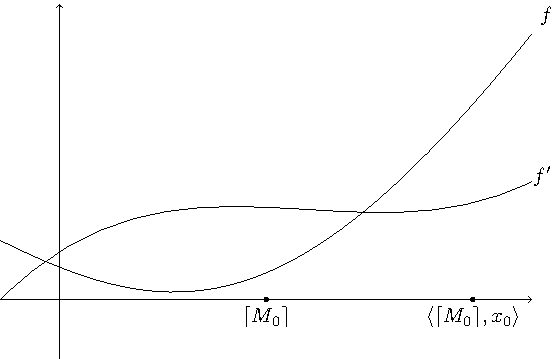
\includegraphics{./img/spacehierarchy.pdf}
            \caption{L'input $\code{M_{0}}$ potrebbe essere in una posizione sfortunata. In generale
            non possiamo fare assunzioni su dove si trovi. La soluzione e' usare un $x$ che sposti
            piu' in la' l'input, dove abbiamo la certezza che $f$ sia al di sopra di $f'$}
            \label{img:spacehierarchy}
        \end{center}
    \end{figure}

    Quello che vogliamo e' quindi spostare l'input in un punto tale che da li' in poi $f$ sara'
    definitivamente al di sopra di $f'$. Di fatto noi siamo interessati alla complessita' della
    macchina $M_{0}$, ma sapendo che questa lavora in spazio $O(f')$ avremo che dal punto che
    raggiungiamo con il ``padding'' dato da $x_{0}$ in poi questa lavorera' in uno spazio che sara'
    definitivamente minore di $f$ a meno di una costante.

    %(Sulla registrazione c'e' la spiegazione della validita' di questo claim).
    Ci chiediamo ora se $\pair{\code{M_{0}}}{x_{0}} \in \Lang$. Questo succede sse
    $\pair{\code{M_{0}}}{x_{0}} \in \Lang_{M_{0}}$. Ma questo succede sse, per definizione di
    $\Lang$, $\pair{\code{M_{0}}}{x_{0}} \notin \Lang_{M_{0}} \land
    s_{M_{0}}(|\pair{\code{M_{0}}}{x_{0}}|) \leq f(|\pair{\code{M_{0}}}{x_{0}}|)$. La seconda parte
    della congiunzione e' vera per come abbiamo scelto $x_{0}$, e a questo punto abbiamo una
    contraddizione.

    Dobbiamo ora dimostrare che questo linguaggio e' riconoscibile in spazio $O(f)$. Quando vogliamo
    dimostrare che un certo linguaggio fa parte di una certa classe di complessita' purtroppo l'unico
    metodo che abbiamo e' quello di andare a definire un programma che riconosce il linguaggio con la
    complessita' della classe. Dobbiamo quindi progettare un algoritmo.

    Come procediamo? Prendiamo una stringa $\pair{\code{M}}{x}$. Dovremmo quindi verificare,
    inizialmente, che la prima parte della stringa rappresenti una MdT. Questo e' abbastanza
    semplice, e si puo' fare con dei semplici controlli sintattici. Dopodiche' andiamo a fare
    l'operazione vera e propria di riconoscimento. Proviamo a simulare il comportamento della
    macchina $M$. Ci serve una macchina universale che simuli $M$ su input $\pair{\code{M}}{x}$.
    Dovremmo quindi portare avanti la computazione e, nel caso la macchina $M$ rifiuti, accettare,
    altrimenti rifiutare.

    Abbiamo due problemi: la macchina simulata potrebbe non terminare su quell'input e non sappiamo
    che complessita' abbia la nostra simulazione, percio' potrebbe sforare il limite di $f$.
    Dobbiamo fare una simulazione bound, limitata da una quantita' data in input. 

    Il nostro bound ce lo abbiamo, dalla seconda parte della definizione di $\Lang$. Possiamo
    pensare di ritagliarci uno spazio di dimensione data nei nastri della macchina. Se, durante la
    computazione, la nostra simulazione cerca di sforare il limite possiamo interropompere la
    computazione e dire che la stringa non appartiene nel linguaggio. Siccome diamo bound $f$ al
    simulatore riusciremo ad utilizzarlo con quello spazio, non di piu'. Abbiamo quindi limitato la
    complessita' in spazio.

    Questo concluderebbe la dimostrazione.

    La parte cruciale della dimostrazione e' la simulazione bound della macchina $M$. Nell'emulare
    non abbiamo un problema legato alla memorizzazione della macchina da emulare, poiche' questo
    richiede una quantita' lineare nella dimensione dell'input. Per dare l'upper bound alla macchina
    simulata e' sufficiente dare questo upper bound allo spazio dedicato alla memorizzazione dei
    nastri simulati nell'emulatore.

    Resta una piccola problematica. Possiamo si' dare un upper bound allo spazio, ma cio' non
    implica che la macchina che stiamo simulando termini. Il problema sorge perche' se la macchina
    emulata non termina noi dovremmo accettare, non dovremmo divergere. La limitazione in spazio non
    ci aiuta, perche' la nostra macchina puo' divergere anche senza sforare il limite.

    Dobbiamo utilizzare il teorema sulla relazione tra tempo e spazio per dare un upper bound anche
    al tempo. Se la macchina simulata non termina la sua computazione entro il tempo dato allora
    rifiuta l'input, e quindi l'emulatore accetta. Dobbiamo quindi memorizzare un timer e
    decrementarlo ad ogni operazione della macchina simulata. Se questo raggiunge lo 0 allora la
    macchina simulata e' in loop e noi dobbiamo accettare.

    Quanto occupa il timer? Il timer ha valore esponenziale rispetto allo spazio, ma noi lo
    rappresentiamo come un numero. Di conseguenza avra' un'occupazione logaritmica rispetto al suo
    valore. Ci serve quindi un'occupazione di memoria dell'ordine $O(f)$. 
\end{proof}

Nella dimostrazione abbiamo omesso un dettaglio: $f$ deve essere costruibile in spazio. Noi
prendiamo l'input e, in base alla sua dimensione e attraverso $f$, allochiamo la memoria che fa da
bound. Ma questo calcolo per l'allocazione richiede uno spazio limitato da $f$? Non possiamo avere
questa garanzia in generale, da cui la necessita' che $f$ sia costruibile in spazio.

\begin{defn}
    Una funzione $f:\Nat \to \Nat$ e' detta costruibile in tempo se esiste una MdT $M$ sull'alfabeto
    $\Sigma = \set{0}$ che calcola una funzione $f_{M}$ per cui:
    \begin{itemize}
        \item per ogni $n$, $f_{M}(0^{n}) = 0^{f(n)}$
        \item $t_{M} \in O(f)$.
    \end{itemize}
    Analogamente, $f$ e' costruibile in spazio se valgolo le stesse condizioni con $s_{M}$ al posto
    di $t_{M}$.
\end{defn}

Questo significa che il calcolo di $f$ deve poter essere fatto in $O(f)$. Tutte le funzioni
semplici sono tipicamente costruibili: un polinomio lo costruiamo in tempo polinomiale, un
esponenziale in tempo esponenziale, ecc. Ci sono pero' funzioni $f$ che hanno delle
complicazioni tali che $f$ richiede piu' di $O(f)$ spazio per essere calcolata.

Di solito quando parliamo di classi di complessita' come $\DSPACE(f)$ e $\DTIME(f)$, affinche'
abbiano senso, richiediamo almeno che la $f$ sia costruibile, per non creare delle situazioni
strane.  Si puo' dimostrare che senza questa ultima ipotesi il teorema sarebbe falso. Ovvero, si
puo' dimostrare che se abbiamo due funzioni non costruibili $f,g$, con $g \in o(f)$, possiamo avere
un gap con nessun linguaggio in mezzo.

%Ad esempio, possiamo avere $f \in o(g)$ con nessun linguaggio tra $g$ e $f$  ($g$ e $f$ non
%costruibili).
%
Ad esempio il logaritmo non e' una funzione costruibile in tempo: non riusciamo a calcolare il
logaritmo in tempo logaritmico, e' una funzione troppo complicata.

Se usiamo una funzione $f$ per definire una classe di complessita', ovvero vogliamo
raggruppare tutti i problemi risolvibili con una complessita' che ha $f$ come upper bound, ci
aspettiamo che il calcolo di $f$ faccia parte della classe. Ad esempio, $\DTIME(n^{2})$ e' una
classe ragionevole perche la funzione $n^{2}$ e' calcolabile in tempo $n^{2}$. La costruibilita' di
una funzione e' un sanity check che possiamo fare sulle classi di complessita' che definiamo. E' un
po' il motivo per cui non ha senso considerare classi di complessita' sublineari in tempo.

\subsection{Il teorema della gerarchia in tempo}

Il teorema della gerarchia vale anche per il tempo. Tuttavia per il tempo la cosa non e' cosi'
semplice.

\begin{thm}
    Siano $f,f':\Nat \to \Nat$. Si ha che:
    \begin{equation*}
        f' \in o\left(\frac{f}{\log(f)}\right) \implies \DTIME(f') \subset \DTIME(f)
    \end{equation*}
\end{thm}

In questo teorema richiediamo inoltre che $n \in O(f')$, ovvero $f'$ sia maggiore o uguale
all'identita'.

Cosa cambia col tempo? La prima parte della dimostrazione non cambia, dato che nella prima parte non
abbiamo posto molta attenzione sul tipo di risorsa usata. Il fatto che usassimo lo spazio piuttosto
che il tempo non entrava praticamente in gioco. Il problema e' nella seconda parte, ovvero
nella simulazione con un bound in tempo. Determinare il costo della simulazione comporta qualche
complicazione ulteriore.

In una simulazione bound in tempo abbiamo una macchina e una limitazione in tempo e vogliamo che la
macchina venga simulata con il vincolo in tempo dato. Abbiamo una complicazione dovuta alla gestione
del bound. E' una computazione piu' difficile da gestire di quella di una macchina universale, che
data la macchina e un input esegue la computazione senza alcun vincolo.

Abbiamo quindi un rallentamento nella simulazione bound in tempo, ma di che tipo? Abbiamo
sicuramente un rallentamento vistoso dovuto al fatto che con l'emulatore dobbiamo andare a cercare
la prossima istruzione della macchina emulata. In effetti questo mostra un aspetto un po'
criticabile della teoria della complessita', in cui una macchina di Turing consuma con costo 1 il
programma e, ``magicamente'', trova istantaneamente la quintupla corrispondente alla prossima
istruzione da eseguire ad ogni passo della computazione. La ricerca delle istruzioni da eseguire in
memoria fatta dall'emulatore corrisponde ad una situazione gia' piu' realistica.

Questa ricerca e' limitata in tempo dalla dimensione del programma. Possiamo considerare questa
costante, che dipende da programma a programma, ma sicuramente non dipende dall'input. Avremo quindi
un costo aggiuntivo $M$, ma dal punto di vista della complessita' non ci cambia niente.

Tuttavia nella simulazione bound dobbiamo anche gestire un timer da decrementare ad ogni operazione.
Questo ha una dimensione logaritmica rispetto al valore del timer. Di conseguenza dobbiamo tenere
conto, nel programma simulato, di un rallentamento logaritmico dovuto alla gestione del timer. Se il
nostro bound era $f(x)$ avremo una complessita' $f(x)\log(f(x))$. Sebbene il timer decresca col
tempo questo non cambia l'ordine di grandezza del rallentamento.

Di conseguenza non riusciamo a garantire la seconda parte della definizione di $\Lang$, dobbiamo
aumentare il gap. Abbiamo bisogno che $O(t') \subseteq O(\frac{t}{\log(t)})$. Poiche' abbiamo un
rallentamento logaritmico avremo che invece di operare in tempo $t$ la nostra simulazione operera'
in tempo $t\log(t)$, se $t$ era il bound che diamo alla nostra simulazione. Se alla simulazione
diamo un buond $\frac{t}{\log(t)}$ avremo che la simulazione avra' costo $\frac{t}{\log(t)}\cdot
\log\left(\frac{t}{\log(t)}\right) \leq \frac{t}{\log(t)}\cdot \log(t) \leq t$, e riusciremo a farla in un
tempo $O(t)$.

%\begin{figure}[h]
%    \begin{center}
%        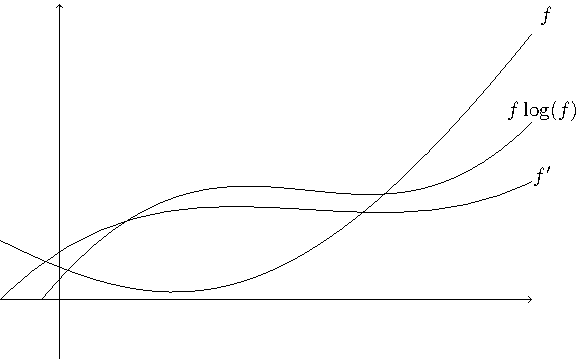
\includegraphics{./img/timehierarchy.pdf}    
%        \caption{Affinche' un linguaggio sia riconoscibile in $O(f)$ ma non in $O(f')$ richiediamo
%        che $f' \in o\left(\frac{f}{\log(f)}\right)$. Si congettura che questo gap logaritmico
%        ulteriore non sia necessario, ma cio' non e' ancora stato dimostrato.}
%    \end{center}
%\end{figure}

Allo stato attuale della conoscenza non riusciamo ad essere piu' precisi al riguardo. Tuttavia non
e' stato dimostrato che non si possa essere piu' precisi in questa classificazione. Questo pero'
non ci cambia molto dal punto di vista delle gerarchie: rimane l'inclusione stretta tra classi di
complessita' come, ad esempio, $\DTIME(n)$ e $\DTIME(n^{2})$, e $\PClass$ e $\EXP$.

Anche in questo caso richiediamo la costruibilita' in tempo della funzione che calcola il valore del
timer che fa da upper bound.

In tempo non riusciamo a fare classi cosi' fini come riusciamo in spazio.

Abbiamo che se $f' \in o(\frac{f}{\log(f)})$ allora abbiamo un linguaggio $\Lang$ riconoscibile in
tempo $O(f)$ ma non in tempo $O(f')$.

\section{Alcune gerarchie di complessita'}

Definiamo alcune classi di complessita' come segue:
\begin{itemize}
    \item $\PClass = \displaystyle\bigcup_{c \in \Nat}\DTIME(n^{c})$
    \item $\EXP = \displaystyle\bigcup_{c \in \Nat}\DTIME(2^{cn})$
    \item $\LOGSPACE = \DSPACE(log)$
    \item $\PSPACE = \displaystyle\bigcup_{c \in \Nat}\DSPACE(n^{c})$
    \item $\EXPSPACE = \displaystyle\bigcup_{c \in \Nat}\DSPACE(2^{cn})$
\end{itemize}

Sappiamo che $\DTIME(2^{n})$ e' diversa da $\DTIME(2^{2n})$, per il teorema della gerarchia in
tempo.  Un'altra possibile definizione di $\EXP$ e' data dall'unione, su tutti i polinomi $p$, di
$\DTIME(2^{p})$. Sono due definizioni diverse, quest'ultima contiene la prima.

Abbiamo le seguenti relazioni tra queste classi di complessita':
\begin{itemize}
    \item $\LOGSPACE \subseteq \PClass \subseteq \PSPACE \subset \EXPSPACE$
    \item $\LOGSPACE \subset \PSPACE$
    \item $\PClass \subset \EXP \subseteq \EXPSPACE$
\end{itemize}

Per le inclusioni strette ci sono delle dimostrazioni, per quelle non strette non
sappiamo se siano strette.

Perche' $\LOGSPACE$ e' incluso in $\PClass$? I teoremi della gerarchia si applicano a classi uniformi di
complessita' (spazio vs spazio, tempo vs tempo). Con $\PClass$ e $\LOGSPACE$ stiamo confrontando risorse
diverse, e percio' il teorema della gerarchia non si applica. Abbiamo che $\LOGSPACE$ contiene tutti
linguaggi riconoscibili in spazio $O(\log(n))$. Per il teorema tempo-spazio abbiamo che un
linguaggio con quella complessita' in spazio e' riconoscibile con una complessita' in tempo
$O(2^{c\cdot(\log(n) + \log(n))}) = O(2^{c'\log(n)})$, per qualche $c'$. Ma $O(2^{c'\log(n)}) =
O(n^{c'})$, quindi abbiamo una complessita' poliomiale in tempo, e quindi il nostro linguaggio fa
anche parte di $\PClass$.

\section{Padding}

Il padding e' l'unica altra tecnica nota, oltre al teorema della gerarchia, per separare classi di
complessita'.

Il padding e' una trasformazione tra linguaggi. Abbiamo $\Lang$ e lo trasformiamo in $\LPad$.
Il linguagggio $\LPad$, ovvero il linguaggio delle stringhe paddate, e' cosi' definito:
\begin{equation*}
    \LPad = \set{x\#^{f(x)} \mid x \in \Lang}
\end{equation*}
A seconda della funzione $f$ cambia il padding.
\begin{equation*}
    x \mapsto x\overbrace{\#\#\cdots\#}^{f(x)}
\end{equation*}

L'obiettivo e' ingrandire la dimensione delle stringhe del linguaggio. Possiamo fare qualunque tipo
di padding; di solito si fa un padding quadratico. E' un'operazione di ``imballaggio'' delle
stringhe di $\Lang$ con un numero di simboli in piu'.

Ad esempio, se vogliamo un linguaggio con padding quadratico avremmo
\begin{equation*}
    \LPad = \set{x\#^{|x^{2}| - |x|} \mid x \in \Lang}
\end{equation*}

Supponiamo di avere $\Lang$ e $\LPad$. Qual e' piu' semplice da riconoscere? $\LPad$. Per
riconoscere $\LPad$, ovvero decidere se una stringa paddata $w$ sta in $\LPad$, possiamo estrarre
$x$ da $w$ e verificare se $x \in \Lang$ con il riconoscitore di $\Lang$. La rimozione del padding
da $w$ ha costo lineare rispetto a $|w|$, e' un'operazione semplice. Riconoscere $x$ ha una certa
complessita' che dipende dalla dimensione di $x$. Tuttavia noi abbiamo ingrandito l'input: la
dimensione di $w$ e' sicuramente maggiore di quella di $x$. Di conseguenza la complessita' di
verificare se $w \in \LPad$, che calcoliamo rispetto alla dimensione di $w$, puo' essere minore
della complessita' richiesta per verificare se $x \in \Lang$, a seconda del tipo di padding che
abbiamo fatto. 

Abbiamo questo fenomeno: gonfiando opportunamente l'input la complessita' degli algoritmi sembra
diminuire.

Se ad esempio usiamo una notazione in base 1 per i numeri allora tutti gli algoritmi sembrano
migliorare drasticamente a livello di complessita'. Ma questo miglioramento e' fittizio, ed e'
legato all'esplosione esponenziale della dimensione dell'input.

Tipicamente abbiamo uno speedup se calcoliamo la complessita' del riconoscimento del linguaggio
paddato, proporzionale alla nuova dimensione dell'input.

Supponiamo, ad esempio, che la complessita' richiesta per riconoscere $x$ sia $O(|x^{2}|)$.
Supponiamo di fare un padding quadratico, ovvero di passare a $w$ con dimensione $|x^{2}|$. La
complessita' dell'algoritmo di riconoscimento diventa $O(|w|)$, e sembra lineare. Tutto questo
discorso suppone che estrarre $x$ da $w$ sia un'operazione di costo lineare.

\begin{figure}[h]
    \begin{center}
        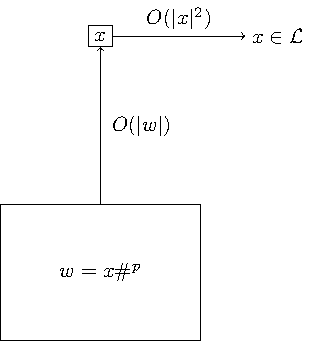
\includegraphics{./img/PaddingSpeedup.pdf}    
        \caption{Riconoscere $\LPad$ costa in genere di meno di riconoscere $\Lang$}
    \end{center}
\end{figure}

Perche' e' interessante il padding? Perche' ci puo' aiutare a separare classi di complessita'. 

Supponiamo di avere due classi di complessita' che vogliamo separare: $\CClass$ e $\CClass'$. Quando
vogliamo capire se due classi sono distinte ci possiamo chiedere rispetto a quali operazioni sono
chiuse.

Le trasformazioni prendono in input un linguaggio e ne restituiscono in output un altro. Che una
trasformazione produca un linguaggio all'interno della classe in cui si trovava il linguaggio di
input non e' ovvio, e quando succede per ogni linguaggio della classe diciamo che la classe e'
chiusa rispetto a questa trasformazione.

Un modo per separare le classi di complessita' e' prendere un'operazione, ad esempio il padding, e
verificare se una delle due e' chiusa rispetto ad essa mentre l'altra non lo e'. Con questo abbiamo
la dimostrazione che le due classi sono diverse.

\begin{figure}[h]
    \begin{center}
        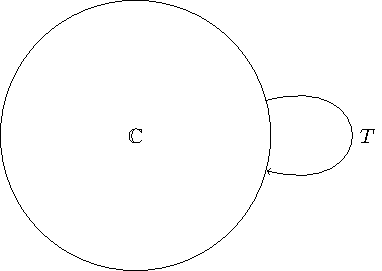
\includegraphics{./img/ClosedClass.pdf}    
        \caption{La classe $\CClass$ in figura e' chiusa rispetto alla trasformazione $T$}
    \end{center}
\end{figure}

Prendiamo $\PSPACE$ e $\EXP$. La nostra $\EXP$ e l'unione dei $\DTIME(2^{cn})$ per ogni $c \in
\Nat$. Si puo' definire $\EXP_{p}$ come l'unione di $\DTIME(2^{n^{c}}$ per ogni $c \in \Nat$. Sono
due classi diverse. Abbiamo che $\EXP \subset \EXP_{p}$: lo si dimostra con il teorema della
gerarchia.

Ci aspettiamo una relazione tra $\PSPACE$ ed $\EXP$? Si'. Per il teorema tempo spazio uno spazio
polinomiale implica un tempo esponenziale. Il grado dell'esponente, pero', dipende dal polinomio.
Sicuramente $\PSPACE \subseteq \EXP_{p}$. Riusciamo a dimostrare altro? Non riusciamo a dimostrare
$\PSPACE \subset \EXP_{p}$ allo stato attuale dell'arte, anche se si suppone cio'. Si riesce a
dimostrare che $\PSPACE \not= \EXP$. Questo perche' abbiamo che $\PSPACE$ e' chiusa rispetto al
padding polinomiale, mentre $\EXP$ non lo e'. Abbiamo inoltre che $\EXP_{p}$ e' chiusa
rispetto ad un certo tipo di padding.

\begin{figure}[h]
    \begin{center}
        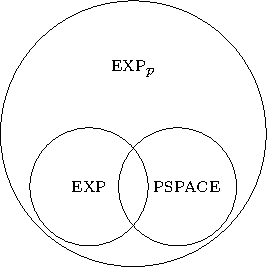
\includegraphics{./img/ExpvsExppvsPSpace.pdf}
        \caption{Gerarchia congetturata tra le classi $\PSPACE$, $\EXP$ e $\EXP_{p}$}
    \end{center}
\end{figure}

\begin{thm}
    $\EXP \not= \PSPACE$
\end{thm}
\begin{proof}
    
    Dimostriamo innanzitutto che $\EXP \subset \DTIME(2^{n^{2}})$. Infatti abbiamo che $\forall c
    \in \Nat, 2^{cn} \in o(2^{n^{2}})$. L'unione di classi tutte contenute in $\DTIME(2^{n^{2}})$
    sta ancora in $\DTIME(2^{n^{2}})$. Dato che $\EXP$ e' definita come il limite di questa unione
    potrebbe essere uguale a $2^{n^{2}}$, di conseguenza non ci basta l'ipotesi di prima per
    concludere $\EXP \subset \DTIME(2^{n^{2}})$. Ce ne serve una piu' forte: consideriamo
    $\DTIME(2^{n^{1.5}})$. Abbiamo che $\forall c,2^{cn} \in o(2^{n^{1.5}})$, e $\DTIME(2^{n^{1.5}})
    \subset \DTIME(2^{n^{2}})$ per il teorema della gerarchia. Di conseguenza $\EXP \subset
    \DTIME(2^{n^{2}})$

    Data questa inclusione stretta abbiamo che $\exists \Lang, \Lang \in \DTIME(2^{n^{2}}) \land
    \Lang \notin \EXP$. Consideriamo ora $\LPad$ con padding quadratico:
    \begin{equation*}
        \LPad = \set{ x\#^{|x|^{2}-|x|} \mid x \in \Lang}
    \end{equation*}

    Supponiamo per assurdo che $\PSPACE = \EXP$. Ci chiediamo ora, qual e' la classe di complessita'
    di $\LPad$? Di quanto decrescera' la complessita' di riconoscere $\LPad$ rispetto alla
    complessita' di riconoscere $\Lang$? Per riconoscere $\LPad$ noi partiamo da una stringa $w$ con
    una certa dimensione $|w|$. Da questa estraiamo, con complessita' lineare, $x$, con lunghezza
    $n$ (da cui $|w| = n^{2}$). Cosa dobbiamo fare per vedere se $w \in \LPad$?  Verificare se $x
    \in \Lang$, con costo $O(2^{n^{2}})$. La complessita' complessiva diventa $O(2^{|w|})$, ovvero
    con esponente lineare in $|w|$. Abbiamo quindi che $\LPad \in \DTIME(2^{n})$, il che implica che
    $\LPad \in \EXP$. Ma questo implica  $\LPad \in \PSPACE$ per la nostra ipotesi di assurdo.

    \begin{figure}[h]
        \begin{center}
            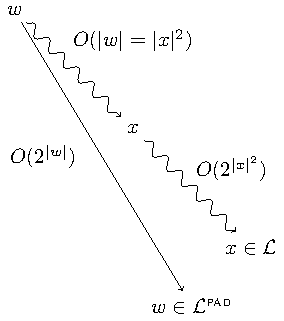
\includegraphics{./img/PaddingCheat.pdf}
            \caption{Riconoscere $\LPad$ ha una complessita' che ci permette di posizionarlo in
            $\EXP$ grazie al padding quadratico}
        \end{center}
    \end{figure}

    Cosa possiamo dire della complessita' in tempo di riconoscere $\Lang$ sapendo che $\LPad \in
    \PSPACE$? Cosa dobbiamo fare per riconoscere $\Lang$ sotto questa ipotesi? Ci basta prendere
    $x$, paddarlo e darlo in pasto all'algoritmo di riconoscimento di $\LPad$. Il padding richiede
    tempo quadratico, il riconoscimento di $\LPad$ lo facciamo in uno spazio in $\PSPACE$.

    \begin{figure}[h]
        \begin{center}
            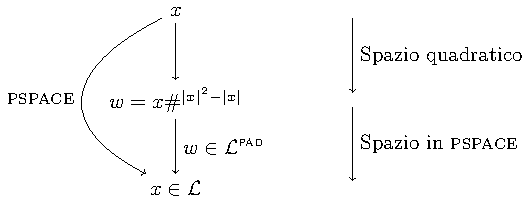
\includegraphics{./img/LPadComplexity.pdf}
            \caption{Sapendo che $\LPad \in \PSPACE$ riusciamo a concludere che anche $\Lang$
            appartiene a $\PSPACE$}
        \end{center}
    \end{figure}

    Qua non possiamo fare il massimo tra le due operazioni per calcolare la complessita' totale,
    dato che la stringa da cui partiamo e' piu' piccola di quella paddata, e il padding ci costa.
    Cio' che conta pero' e' che la composizione di polinomi e' un polinomio, di conseguenza il
    processo usa uno spazio in $\PSPACE$.

    Di conseguenza $\LPad \in \PSPACE \implies \Lang \in \PSPACE \implies \Lang \in \EXP$, il che
    contraddice la nostra ipotesi iniziale.
\end{proof}

In questo caso abbiamo dimostrato che $\EXP \not= \PSPACE$ per assurdo. Si potrebbe anche dimostrare
facendo vedere che $\PSPACE$ e' chiusa rispetto al padding polinomiale mentre $\EXP$ non lo e'.

\subsection{Complessita' della composizione di funzioni}

Sapendo qualcosa su due funzioni $f$ e $g$ sappiamo dire quanto ci costa calcolare $f(g(x))$? Non e'
banale, perche' la complessita' la misuriamo rispetto alla dimensione dell'input. Ci chiediamo
quindi prima quale l'ordine di grandezza degli output di $g$. Se lo sappiamo possiamo calcolare la
complessita' di $f(g(x))$ usando la complessita' di $f$, altrimenti no. Se gli output di $g$ fossero
costanti in dimensione non avrebbe neanche senso chiedersi quale sia la complessita' di $f \comp g$,
dato che sarebbe sempre costante. A noi interessa la complessita' di funzioni che prendono input che
possono crescere arbitrariamente.

Ad esempio, $g$ potrebbe produrre liste e $f$ potrebbe ordinarle. Supponiamo che $g$, data una
lista, produca il suo prodotto cartesiano. Supponiamo che $g$ non restituisca risultati ordinati.
Avremo un output di $g$ di dimensione $n^{2}$. In questo caso avremmo una complessita' $O(n^{2} +
n^{2}\log(n^{2})) = O(n^{2}\log{n})$.

Se noi conosciamo solo la complessita' in tempo possiamo dire qualcosa sulla dimensione degli
output? Con il teorema tempo spazio sappiamo che gli output prodotti sono bound dal tempo richiesto
dall'algoritmo. Non possiamo dare bound migliori per il caso pessimo.

(Figura 7)

Bisogna stare attenti a capire se gli algoritmi producono strutture dimaniche. In tal caso c'e' una
complicazione nel calcolo della complessita' di una funzione composta. E' un'analisi delicata.

\section{Conclusioni}

Volendo riassumere i risultati noti riguardanti le relazioni tra alcune classi di complessita'
possiamo utilizzare un diagramma come quello in figura $\ref{img:detclassesrelations}$. 

\begin{figure}[h]
    \begin{center}
        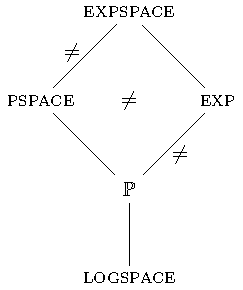
\includegraphics{./img/ComplexityDiagram.pdf}
        \caption{Relazioni di inclusioni tra alcune classi di complessita'}
        \label{img:detclassesrelations}
    \end{center}
\end{figure}

Nel diagramma le linee vanno intese come inclusioni. Con il $\not=$ abbiamo un'inclusione stretta.

Se abbiamo a che fare con risorse dello stesso tipo possiamo usare il teorema della gerarchia per
dire qualcosa riguardo l'inclusione tra due classi di complessita'.

Nel caso abbiamo a che fare con risorse di tipo diverso dobbiamo usare altri strumenti. Ad esempio
il teorema tempo spazio ci permette di stabilire inclusioni tra classi di complessita' in tempo e
spazio.

Il teorema della gerarchia ci puo' dare inclusioni strette, quello tempo spazio da' solo inclusioni
lasche.

Il teorema tempo spazio ci da', se abbiamo un bound polinomiale allo spazio, un bound esponenziale al
tempo di cui non conosciamo la costante.

Ad esempio, se abbiamo un algoritmo che lavora in spazio logaritmico abbiamo che lavorera' in tempo
polinomiale. Di questo polinomio pero' non possiamo sapere, in generale, il grado.

Nel parlare di classi ``feasible'', ovvero con complessita' ragionevole, a volte si tende ad
escludere $\PClass$, perche' risulta troppo grande, includendo problemi con complessita' polinomiale
alta. Si preferisce quindi spesso restringersi a $\LOGSPACE$. In realta' anche questa non e' ideale,
dato che ci possono essere algoritmi che lavorano in spazio logaritmico ma in tempo polinomiale con
un polinomio di grado alto. Inoltre esistono linguaggi riconoscibili in tempo polinomiale basso ma
che usano uno spazio piu' che logaritmico, che in questo caso vengono esclusi. In ogni caso
$\LOGSPACE$ resta una classe interessante che sta completamente in $\PClass$. Si congettura che
$\LOGSPACE \subset \PClass$, ma non si e' ancora riusciti a dimostrarlo. 

$\PSPACE$ e' molto piu' grande di $\NPClass$. Abbiamo infatti che $\PClass \subseteq \NPClass
\subseteq \PSPACE$, ma non si e' ancora dimostrato $\PClass \not= \PSPACE$, nonostante lo si
congetturi.

Le inclusioni del diagramma che non sono strette sono inclusioni che sono congetturate essere
strette ma che non sono ancora state dimostrate esserlo. Le maggior parte delle inclusioni strette
vengono dai teoremi della gerarchia. La relazione tra $\EXP$ e $\PSPACE$ e' invece dimostrabile
sfruttando il padding.

Il bound esponenziale dato dallo spazio al tempo e' interessante perche', ad esempio, ci permette di
stabilire che $\LOGSPACE \subseteq \PClass$.

%% tex/nondeterminism.tex
%% Copyright 2019 Andrea Berlingieri
%
% This work may be distributed and/or modified under the
% conditions of the LaTeX Project Public License, either version 1.3
% of this license or (at your option) any later version.
% The latest version of this license is in
%   http://www.latex-project.org/lppl.txt
% and version 1.3 or later is part of all distributions of LaTeX
% version 2005/12/01 or later.
%
% This work has the LPPL maintenance status `maintained'.
%
% The Current Maintainer of this work is Andrea Berlingieri.
%
% This work consists of all files listed in manifest.txt
\chapter{Complessità non deterministica}

\section{Macchine di Turing non deterministiche}

Vediamo un altro modello di calcolo interessante, quello delle Macchine di Turing non
deterministiche.

Una MdT non deterministica è definita in modo analogo alla versione deterministica, con la sola
differenza che la funzione di transizione $\delta$ è multivalore:
\begin{equation*}
    \delta \subseteq Q \times \Sigma^{k} \times \powerset{Q \times \Sigma^{k} \times \set{L,R}^{k}}
\end{equation*}

In altri termini nella MdTN invece di avere una sola quintupla per ogni coppia stato-carattere ne
abbiamo un insieme finito. In un certo senso è come se avessimo un programma che, invece di avere
una singola istruzione con cui continuare, ha un insieme finito di istruzioni tra cui scegliere per
proseguire la sua computazione.

È semplice da definire formalmente, basta modificare la definizione della macchina deterministica.
La macchina deterministica è in un certo senso più difficile da definire formalmente rispetto alla
versione non deterministica, dato che la si può definire ponendo dei vincoli alla definizione di
quest'ultima.

La macchina deterministica rappresenta un caso particolare della macchina non deterministica dove la
scelta della quintupla è univoca. Se qualcosa è calcolabile da una macchina deterministica lo è
anche da una non deterministica. Di conseguenza le classi deterministiche sono contenute nelle
corripondenti classi non determistiche. Ad esempio, $\PClass \subseteq \NPClass$, $\PSPACE \subseteq
\NPSPACE$, etc.

Definire la MdTN è semplice. È più complicato definire cosa calcola la MdTN. In una MdTN è
facile capire che ci sono più computazioni possibili. Quale sia però il risultato calcolato dalla
macchina non è ovvio.

Noi ci restringiamo a considerare solamente macchine decisionali, ovvero che rispondono sì/no.
Queste ci sono sufficienti perché siamo interessati a riconoscere linguaggi. Le nostre macchine
terminano con risposta booleana.

Quando possiamo affermare che una stringa è accettata da una MdTN? Abbiamo due criteri. Una stringa
può essere accettata dalla MdTN se, qualunque computazione della macchina venga fatta, la stringa
viene sempre accettata, oppure può essere accettata se esiste una computazione che accetta la
stringa. A noi interessa la seconda definizione, quella della ``macchina fortunata'': ogni volta che
abbiamo una scelta la nostra macchina fa quella giusta.

%Se esiste una computazione della MdTN che porta al riconoscimento la stringa è considerata
%riconosciuta. // Ripetizione

La computazione della macchina può essere rappresentata da un grafo.

\begin{figure}[h]
    \begin{center}
        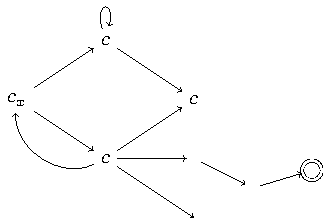
\includegraphics{./img/nondeterminism/MdTN.pdf}
        \caption{Grafo delle computazioni di una MdTN}
    \end{center}
\end{figure}

Il grafo è diretto non necessariamente aciclico. Il numero di scelte è finito e definito dalla
macchina (dal programma), che è finita. Il grafo non è neanche necessariamente finito, dato che
possono esistere computazioni che non terminano non cicliche.

Ci porremo più avanti il problema di simulare la MdTN, e qui ci tornerà utile questo grafo, detto
grafo delle computazioni.

Alcuni cammini nel grafo portano a stati finali accettanti, altri no, altri possono andare avanti
indefinitamente. A noi basta che esista un cammino che porti ad una configurazione di accettazione
per riconoscere una stringa.

%La nostra definizione di accettazione ci permetterà di avere delle relazioni con l'esistenza di un
%certificato.

Consideriamo $\SAT$. Come funzionerebbe la MdTN per $\SAT$? Noi dobbiamo prendere una formula
proposizionale e decidere se questa è soddisfacibile. La nostra macchina comincia a leggere la
formula e trova come prima variabile proposizionale, ad esempio, $A$. $A$ è vera o falsa? La
macchina ``tira una moneta'' e decide il valore di verità di $A$. Dopodiché la macchina va avanti.
Questo processo continua fino alla fine della formula. Se la formula è soddisfacibile esiste almeno
una computazione fortunata che indovinerà l'assegnazione giusta di valori di verità alle variabili
proposizionali.

Alla macchina non deterministica basta una scansione lineare della formula, e quindi riesce a
risolvere $\SAT$ in tempo lineare, a patto di prendere la strada giusta. $\SAT$ è risolvibile in
tempo polinomiale non deterministico da una MdTN. Questa sarà anche il modo in cui definiremo la
classe $\NPClass$.

\section{Complessità non deterministica}

Dobbiamo definire quali sono il tempo e lo spazio consumati dalla MdTN durante una computazione. Se
la macchina accetta l'input esiste una computazione accettante. Se la risorsa che consideriamo è il
tempo noi prendiamo il tempo della computazione accettante più corta. In termini del grafo delle
computazioni prendiamo il più corto cammino accettante della MdTN e la lunghezza di quel cammino è
il numero di passi richiesto per riconoscere una stringa $x$. Questo numero rappresenta quindi il
tempo richiesto dalla macchina. Indichiamo il tempo richiesto dalla MdTN $M$ su input $x$ con
$\textit{time}_{M}(x)$.

Analogamente per lo spazio prendiamo lo spazio minimo tra gli spazi richiesti dalle computazioni
accettanti. Tuttavia bisogna fare attenzione al come calcoliamo lo spazio richiesto da una
computazione. Questo corrisponde al massimo spazio usato in una configurazione della computazione.
Dobbiamo considerare il ``minimo dei massimi''. Indichiamo lo spazio richiesto dalla MdTN $M$ su
input $x$ con $\textit{space}_{M}(x)$.

Le funzioni $t_{M}$ e $s_{M}$ sono definite identicamente a come lo erano nel caso deterministico, a
patto di usare le nozioni di $\textit{time}$ e $\textit{space}$ appena definite. Un discorso analogo
si applica alle definizioni di $\NTIME(f)$ e $\NSPACE(f)$.

Possiamo definire le classi $\NPClass$, $\NEXP$, $\NLOGSPACE$ e $\NPSPACE$ in maniera identica a
come abbiamo definito le corrispondenti classi deterministiche, avendo cura di usare $\NTIME$ al
posto di $\DTIME$ e analogamente per lo spazio.

Possiamo formalizzare quanto detto prima sulla relazione tra macchine di Turing deterministiche e
non deterministiche con il seguente teorema.
\begin{thm}
    Per ogni $f: \Nat \to \Nat$
    \begin{equation*}
        \DTIME(f) \subseteq \NTIME(f) \land \DSPACE(f) \subseteq \NSPACE(f)
    \end{equation*}
\end{thm}
La dimostrazione è ovvia essendo la macchina di Turing deterministica un caso particolare della
macchina non deterministica.

%(Abbiamo saltato la riduzione dei nastri)

\section{Simulazione del non determinismo}

Vogliamo stabilire delle relazioni tra la MdTN e la corrispondente macchina deterministica. Per
stabilire queste relazioni una tecnica che risulta utile è pensare in termini di simulazione.
Siamo quindi interessati a teoremi che riguardano la simulazione del nondeterminismo.

Immaginiamo di avere una macchina non deterministica che riconosce un linguaggio con una certa
complessità e immaginiamo di simularla con una macchina deterministica. Se riusciamo a determinare
la complessità della simulazione rispetto alla complessità della macchina di partenza riusciamo a
dire qualcosa sulla complessità del riconoscimento del linguaggio in modo deterministico.

C'è un modo interessante di vedere la simulazione della MdTN: consideriamo il grafo delle
computazioni di una MdTN. Per simulare la macchina in modo deterministico ci basta trovare un
algoritmo deterministico di visita dei cammini del grafo. Dobbiamo fare un'esplorazione completa,
dato che possono esistere in generale cammini di riconoscimento migliori di uno già trovato.
Dobbiamo fare una qualche visita astuta per effettuare la simulazione.

%Slide 89

In generale quando vogliamo stabilire delle relazioni tra classi deterministiche e classi non
deterministiche usiamo classi di risorse diverse. Ad esempio, avendo un bound di tempo alla
complessità della MdTN diciamo qualcosa riguardo alla complessità in spazio della simulazione
deterministica. Il primo teorema che vediamo mostra questo.

\subsection{Simulazione di una macchina non deterministica con un bound al tempo}

Supponiamo di conoscere la complessità $O(f)$ in tempo della macchina non deterministica e ci
chiediamo quale sia la complessità in spazio della simulazione deterministica, cercando di
minimizzare l'occupazione di memoria.

Quello che dobbiamo fare è occupare il minor spazio possibile durante la nostra visita del grafo
delle computazioni. La visita in ampiezza non è la migliore scelta in questo caso, dato che in
generale potremmo avere una frontiera attiva dei nodi da visitare molto ampia che non ci è
necessaria.

Abbiamo che la MdTN lavora in $\NTIME(f)$. Abbiamo che $f$ rappresenta la lunghezza massima dei
cammini da esplorare, dato che sappiamo che nostra macchina non deterministica riconosce il nostro
linguaggio in tempo $O(f)$. Rispetto a questa lunghezza dei cammini il numero di nodi che possiamo
avere cresce in generale esponenzialmente: se avessimo, ad esempio, per ogni nodo una scelta
binaria, avremmo $2^{n}$ nodi.

Consideriamo una visita in profondità. Esploriamo il primo cammino, con lunghezza $O(f(|x|))$.
Quante configurazioni incontriamo? $O(f(|x|))$. Possiamo dire qualcosa sulla dimensione di queste
configurazioni?

Abbiamo che anche per la MdTN il tempo fa da bound allo spazio. Per ogni configurazione l'aspetto
che influisce di più sull'occupazione di spazio è la dimensione dei nastri. I nastri crescono, al
massimo, in modo lineare rispetto al tempo. La dimensione dei nastri è bound da $O(f(|x|))$. Per
memorizzare la catena della configurazioni ci serve $O((f(|x|))^{2})$ spazio.

Questo è lo spazio richiesto per la visita di un ramo del grafo. Tuttavia il ramo che stiamo
visitando potrebbe essere un ramo di fallimento, oppure un ramo che diverge. Nel caso fossimo in uno
di questi due casi, una volta raggiunta una configurazione di fallimento o una volta che abbiamo
raggiunto il bound in tempo della MdTN senza accettare possiamo tornare indietro lungo il ramo alla
prima configurazione dove ci è ancora possibile fare una scelta e effettuarne una diversa.
Procediamo quindi per backtracking. In ogni caso l'occupazione di tutti i cammini che esploriamo ha
gli stessi upper bound dati per il primo cammino.

Con una simulazione di questo tipo lo spazio richiesto dalla simulazione deterministica della MdTN
è dell'ordine di $O(f^{2})$.

Possiamo però fare di meglio. Perché?

In generale come facciamo a risparmiare spazio? Possiamo rendere implicite le rappresentazioni
esplicite dei dati, attraverso una descrizione compatta che prenderà tempo al momento
dell'esecuzione ma ci permetterà di risparmiare spazio. Al costo del tempo risparmiamo spazio.
Tutto ciò che ci è oneroso dal punto di vista della memoria lo rendiamo implicito attraverso una
sintesi compatta (ad esempio una compressione). Quando, in fase di esecuzione, avremo bisogno del
dato ci basterà spendere un pò di tempo per estrarlo dalla sua descrizione.

Abbiamo una tecnica analoga per risparmiare tempo a costo dello spazio. Pensiamo, ad esempio, alla
programmazione dinamica con memoization. Manteniamo una tabela per memorizzare le soluzioni dei
sottoproblemi. Quando ci serve una soluzione ad un sottoproblema possiamo guardare la tabella e, nel
caso il sottoproblema sia già stato risolto, ottenere subito il risultato richiesto. Se questo non
è il caso risolviamo il sottoproblema e memorizziamo la soluzione in tabella per usi futuri.

Tempo e spazio sono due risorse ``complementari''. Non si può, allo stesso tempo, ottimizzare il
tempo e lo spazio. Ottimizzare in tempo richiede spendere in spazio e viceversa.  Di solito siamo
portati a pensare a ottimizzazioni del tempo, senza considerare lo spazio.

Quello che occupa più spazio nella nostra visita dei cammini è la memorizzazione esplicita della
catena di configurazioni. Possiamo dare una descrizione del cammino che prendiamo nel grafo molto
più compatta, ad esempio come sequenza di scelte fatte dalla configurazione iniziale. Possiamo
etichettare ogni scelta nel cammino con un numero e salvarci le etichette del nostro cammino.
L'unica informazione che ci serve per definire il cammino è la sequenza delle scelte prese. Nel
caso dovessimo fare backtracking possiamo ripercorrere tutte le scelte del cammino corrente fino
alla scelta da rivedere e cambiare scelta. Considerando tutte le possibili scelte avremo considerato
tutti i possibili cammini del grafo.

Quanto ci costa memorizzare questa sequenza di scelte? L'unica configurazione che teniamo attiva è
quella finale, che è bound da $O(f(|x|))$ per il teorema tempo spazio. Le scelte sono in un range
finito fissato dalla macchina.

In definitiva ci servirà $c\cdot O(f(|x|))$ spazio per memorizzare le scelte e $O(f(|x|))$ per la
configurazione finale del cammino. L'ordine dell'occupazione di spazio della simulazione fatta in
questo modo è quindi $O(f(|x|))$. Riusciamo a fare la simulazione della MdTN in spazio $O(f(x))$.

\begin{thm}\label{thm:ntimedspace}
    Per ogni $f:\Nat \to \Nat$ costruibile in spazio maggiore o uguale all'identità:
    \begin{equation*}
        \NTIME(f) \subseteq \DSPACE(f)
    \end{equation*}
\end{thm}

Possiamo vedere la simulazione in un modo più operazionale. Dato $x$ inizializziamo due nastri di
dimensione $f(|x|)$. In un nastro memorizziamo il tape e in un altro le scelte. All'inizio
simuleremo la computazione dove la scelta che facciamo è sempre la prima. Sul nastro del tape
simuliamo la computazione della MdTN. A questo punto arriviamo in fondo in vari modi: o terminiamo
il tempo, o cerchiamo di sforare lo spazio, o ci arrestiamo con riconoscimento, o ci arrestiamo con
fallimento. In quest'ultimo caso andiamo a cambiare l'ultima scelta per fare backtracking e
rifacciamo la computazione. L'occupazione di spazio rimane dell'ordine $O(f)$. Dovremmo memorizzare
anche un timer per non sforare in tempo, ma questo ha occupazione logaritmica nel valore di $f$. Di
conseguenza l'occupazione di spazio non peggiora.

\begin{figure}[h]
    \begin{center}
        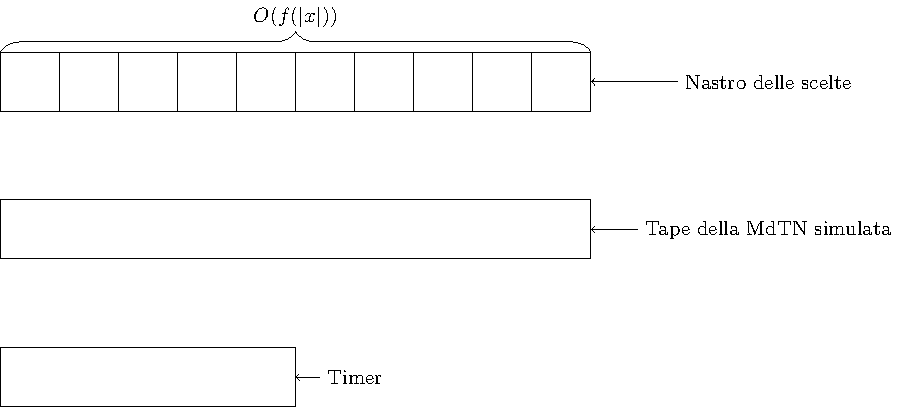
\includegraphics[scale=0.7]{./img/nondeterminism/Simulation.pdf}
        \caption{Simulazione deterministica di una MdTN con memoriazzazione delle scelte}
    \end{center}
\end{figure}

% TODO change all explicit references to "teorema tempo spazio" with a \ref to the right theorem
La simulazione del nondeterminismo non richiede un grande utilizzo di spazio. Il teorema
\ref{thm:ntimedspace} generalizza il teorema tempo spazio: non solo $\DTIME(f)$ è contenuto in
$\DSPACE(f)$, ma anche $\NTIME(f)$. Dal teorema e dall'inclusione $\DTIME(f) \subseteq \NTIME(f)$
deriva il teorema tempo spazio.

\subsection{Simulazione di una macchina non deterministica con un bound allo spazio}

Vediamo ora cosa possiamo dire della complessità in tempo della simulazione di una MdTN che lavora
con una data complessità in spazio.

Sia $M$ una MdTN che riconosce un linguaggio $\Lang \in \NSPACE(f)$ e consideriamo il suo grafo di
raggiungibilità. Possiamo fare un'ipotesi aggiuntiva su questo grafo e dire che esiste un'unica
configurazione finale di riconoscimento. Ciò è diverso dall'affermare che abbiamo un solo stato
finale di riconoscimento. Possiamo fare questa ipotesi perché in generale possiamo ``canonizzare''
tutte le configurazioni finali di una MdTN ``ripulendo'' i nastri, e ottenere una macchina con la
stessa complessità in spazio con un'unica configurazione finale. Questa operazione di
canonicalizzazione degli stati finali richiederà sicuramente del tempo ma non dello spazio
aggiuntivo.

\begin{figure}[h]
    \begin{center}
        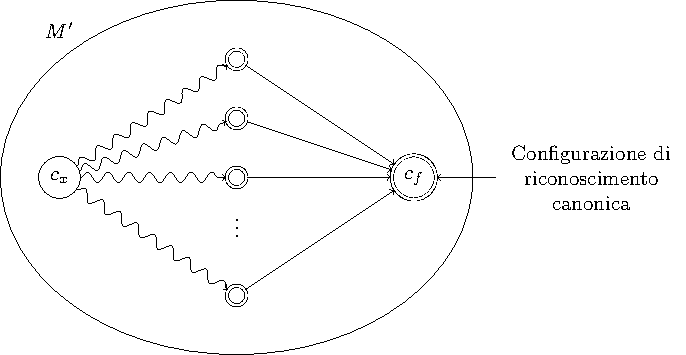
\includegraphics[scale=0.7]{./img/nondeterminism/Canonicalization.pdf}
        \caption{Canonicalizzazione di una MdTN $M$.}
    \end{center}
\end{figure}

Sotto questa ipotesi possiamo vedere la simulazione deterministica di $M$ come la ricerca di un
cammino dalla configurazione iniziale all'unica configurazione finale accettante. La complessità di
questa operazione sarà proporzionale alla dimensione del grafo delle computazioni di $M$.

Possiamo dare un upper bound alla dimensione del grafo? Sì. Cerchiamo di capire quanti sono i nodi
di questo grafo. Gli archi saranno di ordine quadratico rispetto a questa quantità. I nodi sono le
possibili configurazioni finite diverse possibili. Abbiamo che la dimensione dei nastri è $O(f)$.
Sappiamo quante sono le configurazioni possibili dato un bound allo spazio: saranno una quantità di
ordine esponenziale in $f$. Abbiamo quindi che la dimensione del grafo sarà $O(2^{cf})$.

\begin{thm}\label{thm:nspacedtime}
    Per ogni $f:\Nat \to \Nat$ costruibile in spazio maggiore esiste $c \in \Nat$ tale che
    \begin{equation*}
        \NSPACE(f) \subseteq \DTIME(2^{c(\log + f)})
    \end{equation*}
\end{thm}

Il $\log$ nell'esponenziale ci indica, come sempre, che richiediamo che $f$ sia almeno $\geq
\log(n)$. Questo perché consideriamo complessità in tempo almeno lineari.

Anche in questo caso abbiamo una generalizzazione del teorema tempo spazio. Questa generalizzazione
è stretta se supponiamo che $\DSPACE(f) \subset \NSPACE(f)$. Questo, al solito, si congettura ma
non è ancora stato dimostrato. Abbiamo che $\DSPACE(f) \subseteq \NSPACE(f)$, da cui $\DSPACE(f)
\subseteq \DTIME(2^{c(log + f)})$.

Possiamo dire che i teoremi tempo spazio valgono se immaginiamo che dalla parte sinistra delle
inclusioni abbiamo una macchina non deterministica.

Possiamo ora concludere qualcosa riguardo all'utilizzo di risorse dello stesso tipo nella
simulazione di una MdTN.

Supponiamo di avere una MdTN che lavora con complessità in $\NTIME(f)$. Per il teorema
\ref{thm:ntimedspace} abbiamo che $\NTIME(f) \subseteq \DSPACE(f)$. Per il teorema tempo spazio
$\DSPACE(f) \subseteq \DTIME(2^{cf})$, per un $c$ opportuno. Di conseguenza $\NTIME(f) \subseteq
\DTIME(2^{cf})$. Potrebbe andare meglio per casi specifici, ma l'upper bound dato è sempre valido.
Questo risultato non è tanto sorprendente, se consideriamo un tipico grafo delle computazioni di
una MdTN.

Cosa possiamo dire per lo spazio? Abbiamo sicuramente che $\NSPACE(f) \subseteq \DTIME(2^{cf})$, per
un opportuno $c$. Per il teorema tempo spazio abbiamo che $\DTIME(2^{cf}) \subseteq
\DSPACE(2^{cf})$, da cui $\NSPACE(f) \subseteq \DSPACE(2^{cf})$. Questo risultato è meno intuitivo,
dato che lo spazio è una risorsa riutilizzabile. Il tempo, invece, non lo è. Potremmo utilizzare lo
spazio già usato per una computazione per provarne un'altra. Non è ovvio che si possa fare meglio,
ma si può ed è dimostrabile. Inoltre il miglioramento è molto significativo.

\subsection{Teorema di Savitch}

\begin{thm}
    \textbf{(Teorema di Savitch).} Sia $f:\Nat \to \Nat$ una funzione costruibile in spazio e tale
    che $\log \in O(f)$. Allora
    \begin{equation*}
        \NSPACE(f) \subseteq \DSPACE(f^{2})
    \end{equation*}
\end{thm}

Simulare in modo deterministico una computazione non deterministica che richiede spazio $O(f)$ è
fattibile in spazio $O(f^{2})$.

È un teorema importante perché ha un corollario molto rilevante. Una simulazione deterministica di
una MdTN ha un overhead esponenziale in tempo, ma non in spazio. Abbiamo un overhead quadratico.

L'idea è sempre quella di fare una visita del grafo. Supponiamo di essere sotto l'ipotesi di
unicità della configurazione finale accettante. Siamo alla ricerca di un cammino che vada dalla
configurazione iniziale a quella finale cercando di occupare il minor spazio possibile. Solitamente
si adoperano due algoritmi per questa problematica: DFS e BFS. Abbiamo gia analizzato la loro
complessità in tempo, ci chiediamo quale sia la loro complessità in spazio.

Consideriamo DFS. La massima profondità di una visita è uguale al numero dei nodi, visto che
consideriamo cammini aciclici. Possiamo supporre di avere una descrizione compatta di un cammino, ma
sarà sempre lineare nel numero dei nodi in dimensione. Questo discorso si applica anche a BFS. La
frontiera che possiamo ottenere, nel caso pessimo, può avere dimensione pari al numero di nodi del
grafo. Questi due algoritmi hanno un'occupazione di memoria almeno lineare.

Esiste però un algoritmo per questa problematica concettualmente semplice ma con un'occupazione di
memoria sorprendentemente bassa: $O(\log^{2}(n))$, dove $n$ è il numero dei nodi. Questo è lo
spazio aggiuntivo richiesto, ignorando lo spazio richiesto dall'input.

L'algoritmo utilizza una funzione ricorsiva che possiamo chiamare $\REACH$. $\REACH$ prende in input
due nodi $u$ e $v$ e un parametro $i$. Supponiamo che i nodi siano stati numerati e che $u$ e $v$
siano quindi numeri. Il problema che $\REACH$ risolve è determinare se esiste un cammino da $u$ a
$v$ di lunghezza $\leq 2^{i}$.

L'idea è quella di fare una sorta di divide-et-impera. Abbiamo $u$, $v$ e cerchiamo un cammino di
lungheza $\leq 2^{i}$. Se questo esiste possiamo spezzarlo in due cammini di lunghezza $\leq
2^{i-1}$. In questo caso esiste anche un nodo $x$ ed un cammino di lunghezza $\leq 2^{i-1}$ da $u$ a
$x$ e un cammino analogo da $x$ a $v$. Tuttavia non sappiamo quale nodo sia l'$x$ che cerchiamo; di
conseguenza per trovarlo facciamo una ricerca esaustiva su tutti i possibili $x$.

\begin{figure}[h]
    \begin{center}
        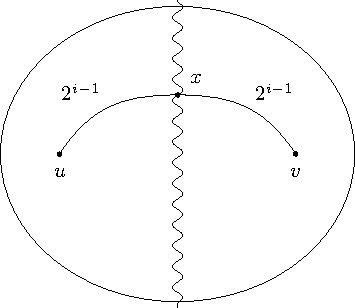
\includegraphics{./img/nondeterminism/SavitchAlgorithm.pdf}
        \caption{Possiamo dividere la ricerca di un cammino di lunghezza $\leq 2^{i}$ nella ricerca
        di due cammini di lunghezza $\leq 2^{i-1}$, utilizzando lo stesso algoritmo.}
    \end{center}
\end{figure}

Lo pseudocodice è illustrato in Algorithm \ref{algo:reach}

\RestyleAlgo{ruled}
\begin{algorithm}
%    \SetNlSty{texttt}{(}{)}
    \caption{\REACH(\textsc{Graph} $G$,\textsc{Node} $u$,\textsc{Node} $v$, \textbf{integer} $i$)}
    \label{algo:reach}
    \If {$i = 0$}
    {
        \Return{$u = v \lor (u,v) \in G.V$}
    }
    \Else
    {
        $\textbf{boolean } res \gets \textbf{false}$

        \ForEach{$x \in G.V$}
        {
            $res \gets res \lor (\REACH(G,u,x,i-1) \land \REACH(G,x,v,i-1)$
        }

        \Return{$res$}
    }
\end{algorithm}

Questo algoritmo è noto come algoritmo di Savitch.

La chiamata iniziale la faremo con un upper bound alla lunghezza massima. Poichè la lunghezza
massima di un cammino aciclico in un grafo è $n$, come valore iniziale per $i$ useremo $\log(n)$:
infatti $2^{\log(n)} = n$.

Discutiamo la complessità in spazio di questo algoritmo. Supponiamo di implementare le chiamate
ricorsive dell'algoritmo mediante uno stack di record di attivazione. Ciò che influisce
sull'occuazione di spazio è il numero massimo di chiamate annidate che possiamo avere e la
dimensione massima dei record di attivazione. Qual è il numero massimo di chiamate annidate? $i$,
dato che ad ogni chiamata l'input decresce. Abbiamo che $i \leq \log(n)$.

Possiamo dare un upper bound anche alla dimensione dei record di attivazione. Nei record di
attivazione abbiamo, in genere, l'input, l'output e le variabili locali. Le variabili di questa
procedura sono, ad esempio, \textit{res} e $x$. Qual'è la dimensione di queste variabili? I nodi
sono dei numeri e la risposta è un booleano. Per memorizzare i nodi ci basta $O(\log(n))$, mentre
per memorizzare la risposta ci è sufficiente uno spazio costante. Avremo un numero costante $k$ di
variabili locali, ma questo non influisce sulla complessità.

Di conseguenza la dimensione richiesta per capire se due nodi sono raggiungibili è dato da $i\cdot
k\log(n) \leq k\log^{2}(n)$, ovvero $O(\log^{2}(n))$. Allo stato dell'arte non si riesce a fare di
meglio a livello di occupazione di spazio.

Qual'è la complessità in tempo di questa procedura? Ricordiamo che abbiamo un trade-off quando
ottimizziamo lo spazio: questa operazione ci costa in tempo. Scriviamo la relazione di ricorrenza:
il tempo $t$ richiesto al passo $i$ è dato da:
\begin{equation*}
    t_{i} =
    \begin{cases}
        \case{d}{se $i = 0$}\\
        \case{N\cdot 2t_{i-1}}{altrimenti}\\
    \end{cases}
\end{equation*}

Il numero di chiamate è $i \leq \log(N)$. Abbiamo quindi una complessità $O((N\cdot 2)^{\log(N)})
= O(N^{\log(N)}2^{\log(N)}) = O(N\cdot N^{log(N)}) = O(N^{\log(N)+1})$. Potevamo ottenere un bound
simile con il teorema tempo spazio.

È un problema aperto della teoria della complessità riuscire a trovare, se esiste, un algoritmo
che stia ``a metà'' tra questo algoritmo, che ottimizzza lo spazio, e un tipico algoritmo di visita
che ottimizza il tempo.

Tornando alla dimostrazione del teorema di Savitch, sappiamo che riusciamo a fare la ricerca di un
cammino dalla configurazione iniziale a quella finale con uno spazio limitato. Qual è la dimensione
del grafo? Se $f$ è il bound asintotico allo spazio abbiamo un numero di configurazioni
$O(2^{cf})$, per un $c$ opportuno. Con questa dimensione del grafo e utilizzando l'algoritmo di
Savitch abbiamo una complessità $\log^{2}(2^{cf}) = (cf)^{2}$, ovvero $O(f^{2})$.

% TODO rivedi registrazione su questo punto
Questa complessità è tale se nell'occupazione di spazio consideriamo solo quello aggiuntivo
richiesto per la computazione, ignorando quello richiesto per memorizzare l'input. Possiamo fare
questa ipotesi perché possiamo lavorare con il grafo in maniera implicita. L'unico momento in cui
ci serve esplicitamente il grafo è nel caso base dell'algoritmo. Abbiamo una configurazione
$c_{u}$, una configurazione $c_{v}$ e ci chiediamo se si può andare, in un passo, da $c_{u}$ a
$c_{v}$. Dal punto di vista dell'occupazione in spazio questo richiede uno spazio uguale al massimo
tra quelli richiesti da $c_{u}$ e da $c_{v}$. L'importante è fissare $M$, di dimensione costante
che dipende dal programma.

Cosa ci dice questo teorema su $\NPSPACE$? Supponiamo di avere un polinomio, ad esempio $n^{2}$.
Supponiamo di voler riconoscere un linguaggio $\Lang \in \NSPACE(n^{2})$. Per il teorema di Savitch
abbiamo che lo stesso linguaggio sta in $\DSPACE(n^{4})$. In generale il quadrato di un polinomio è
ancora un polinomio. Di conseguenza abbiamo che $\NPSPACE \subseteq \PSPACE$. Poichè le macchine
deterministiche sono un caso particolare di macchine non deterministiche, come ulteriore conseguenza
abbiamo che $\NPSPACE = \PSPACE$.

Questo è l'equivalente, a livello dello spazio, del problema $\PClass$ vs $\NPClass$. Se avessimo
un risultato simile per il tempo, ad esempio $\NTIME(f) \subseteq \DTIME(f^{20})$, potremmo
concludere $\PClass = \NPClass$. Tuttavia un risultato del genere probabilmente non è dimostrabile.

Il motivo per cui l'occupazione di spazio dell'algoritmo di Savitch è compatta è che non
memorizziamo nulla delle computazioni già fatte, mentre la complessità in tempo rimane elevata
dato che per ogni coppia di nodi $u$ e $v$ del grafo sarà ripetuta varie volta l'interrogazione
``il nodo $u$ è raggiungibile dal nodo $v$?''.

Non è possibile risparmiare il tempo di queste computazioni memorizzando, ad esempio, i risultati
delle varie interrogazioni in una tabella. Questo perché il numero dei nodi è esponenziale nella
complessità in spazio. La dimensione di questa tabella sarebbe anch'essa esponenziale e non
riusciremmo a lavorare in uno spazio quadratico in $f$. Come sempre se vogliamo risparmiare in
spazio dobbiamo essere disposti a ``spendere'' in tempo, e viceversa.

%Slide 103
\subsection{Gerarchie di complessità}

Possiamo, dati i risultati sulle computazioni non deterministiche, rappresentare le relazioni di
inclusioni mediante la figura \ref{nondeterminism:img:complexity_hierarchy}:

\begin{figure}[h]
    \begin{center}
        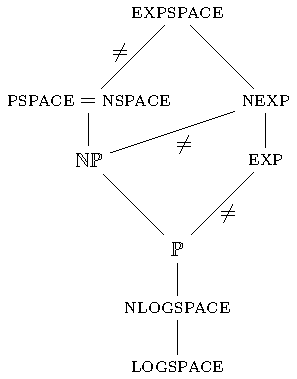
\includegraphics{./img/nondeterminism/Hierarchies.pdf}
        \caption{Rappresentazione delle relazioni di inclusioni note tra alcune classi di
        complessità.}
        \label{nondeterminism:img:complexity_hierarchy}
    \end{center}
\end{figure}

Il significato degli archi e dei segni di disuguaglianza è lo stesso che abbiamo dato per la figura
\ref{timespacehierarchies:img:detclassesrelations}.

Abbiamo che $\LOGSPACE \subseteq \NLOGSPACE$ perché le macchine deterministiche sono un caso
particolare di quelle non deterministiche. Abbiamo inoltre che $\NLOGSPACE \subseteq \PClass$ per il
teorema \ref{thm:nspacedtime}. Sappiamo che $\PClass \subset \EXP$ per il teorema della gerarchia in
tempo, e analogamente abbiamo che $\NPClass \subset \NEXP$. Sappiamo che $\NPClass \subseteq \PSPACE$
per il teorema \ref{thm:nspacedtime} e sappiamo che $\PSPACE = \NPSPACE$ per il teorema di Savitch.
Sappiamo infine che $\PSPACE \subset \EXPSPACE$ per il teorema della gerarchia e che $\NEXP
\subseteq \EXPSPACE$ per il teorema \ref{thm:nspacedtime}.

L'inclusione stretta tra $\NPClass$ e $\NEXP$ non è ovvia. In effetti si può dimostrare che i
teoremi della gerarchia sono generalizzabili al caso non deterministico, e questo giustifica questa
relazione tra le due classi.

%% tex/NPClass.tex
%% Copyright 2019 Andrea Berlingieri
%
% This work may be distributed and/or modified under the
% conditions of the LaTeX Project Public License, either version 1.3
% of this license or (at your option) any later version.
% The latest version of this license is in
%   http://www.latex-project.org/lppl.txt
% and version 1.3 or later is part of all distributions of LaTeX
% version 2005/12/01 or later.
%
% This work has the LPPL maintenance status `maintained'.
%
% The Current Maintainer of this work is Andrea Berlingieri.
%
% This work consists of all files listed in manifest.txt
\chapter{La classe $\NPClass$}

%Slide 105
Vediamo ora due argomenti importanti concentrando la nostra attenzione su una classe di complessita'
molto interessante: $\NPClass$. I due argomenti che trattiamo sono il teorema della proiezione e la
nozione di riducibilita'.

\section{Teorema della proiezione}

Il teorema della proiezione e' importante perche' mette in relazione le due visioni della classe
$\NPClass$: una, che la definisce, e' quella di insieme dei linguaggi riconoscibili da una macchina
non deterministica, e l'altra, interessante a livello pratico, e' quella di insieme dei problemi per
cui esistono algoritmi di verifica della soluzione che operano in tempo polinomiale.

\begin{thm}
    \textbf{(Teorema della proiezione).} Dato un linguaggio $A \subseteq \Sigma^{*}$, $A \in
    \NPClass$ se e solo se esiste un linguaggio $B \in \PClass$ e un polinomio $p$ tale che per ogni
    $x \in \Sigma^{*}$
    \begin{equation*}
        x \in A \iff \exists y, |y| \leq p(|x|) \land \pair{x}{y} \in B
    \end{equation*}
\end{thm}

$y$ e' un certificato che dipende da $x$. E' un'informazione aggiuntiva rispetto ad $x$ che ci
permette di fare una verifica veloce. E' una sorta di ``prova'' che $x$ appartiene in effetti al
linguaggio $A$. L'utilita' di $B$ sta nel fatto che ci permette di verificare in tempo polinomiale
l'autenticita' del certificato per $x$.

Che cosa sia il cerficicato non e' ben definito: dipende dal problema e sta a noi definire cosa sia
un buon cerificato. Dato che noi consideriamo solo problemi decisionali il certificato puo' essere
qualunque informazione che ci permetta di verificare che la risposta sia ``Si'''.

Chiediamo inoltre che la dimensione del certificato non cresca esponenzialmente. Il motivo e' che
input grandi ci danno complessita' basse che sono tuttavia fittizie, un po' come accadeva per il
padding.

Ad esempio per il problema della tautologia abbiamo un algoritmo lineare nella dimensione di una
tabella di verita' che verifica se la tabella e' ben formata, e quindi se una formula data e'
tautologica. Tuttavia questa tabella ha dimensione esponenziale. L'algoritmo risulta efficiente se
confrontato con la dimensione della tabella, ma risulta pessimo se confrontato con la dimensione del
nostro input, ovvero la formula di partenza. Di conseguenza non si tratta di un buon certificato per
noi.

\begin{proof}

    Sia $A \subseteq \Sigma^{*}$, $A \in \NPClass$ e sia $x$ una stringa in $A$. Abbiamo che $A \in
    \NPClass$ sse esiste una MdTN $M$ che riconosce $A$. Che certificato possiamo dare per $x$?
    Come certificato possiamo prendere la sequenza delle scelte prese da $M$ in una computazione che
    riconosce $x$, insieme a $\code{M}$. Quanto e' grande questa sequenza? E' polinomiale in $|x|$,
    essendo $A \in \NPClass$. Esiste quindi un cammino accettante polinomiale nel numero di passi.
    Il codice di $M$ e' costante nella sua dimensione e non influisce a livello della complessita'.
    Sia $B$ il linguaggio delle coppie $x$-certificato. Dato $x$ ed il suo certificato una macchina
    deterministica $M'$ che riconosce il linguaggio $B$ effettua una simulazione di $M$ usando le scelte
    fornite. Se la configurazione finale della simulazione di $M$ e' accettante la machina $M'$
    accetta la coppia $x$-certificato; in caso contrario rifiuta. E' facile verificare il secondo $\iff$
    dell'enunciato del teorema data questa definizione di $M'$ e $B$. Inoltre abbiamo che $B \in
    \PClass$, dato che l'estrazione del certificato dalla coppia e' un'operazione con complessita'
    lineare rispetto alla dimensione di questa e la simulazione di $M$ richiede un numero di passi
    polinomiale in $|x|$.

    Viceversa supponiamo ora di avere $B \in \PClass$. Vogliamo dimostrare che se prendiamo un
    polinomio $p$ e facciamo la proiezione esistenziale bound da $p$ abbiamo che il linguaggio
    ottenuto in questo modo sta in $\NPClass$. In particolare vogliamo dimostrare che il linguaggio
    \begin{equation*}
        A = \set{x \mid \exists y, y \leq p(|x|) \land \pair{x}{y} \in B}
    \end{equation*}
    fa parte di $\NPClass$.

    Per mostrare cio' esibiamo una MdTN $M$ che ci permetta di riconoscere $A$. $M$ funziona nel
    seguente modo: dato $x$ genera tutti i certificati $y$ di dimensione minore o uguale a $p(|x|)$
    e testa l'appartenenza di $\pair{x}{y}$ a $B$ in tempo polinomiale per tutti. Se uno di questi
    certificati risulta valido $M$ accetta $x$, altrimenti rifiuta. La quantita' di certificati da
    testare e' esponenziale, dato che il numero di certificati diversi di lunghezza $p(|x|)$ e'
    $|\Sigma|^{p(|x|)}$. Sfruttando il fatto che la macchina deterministica e' ``fortunata''
    generiamo non deterministicamente il certificato corretto per $x$. $M$ riconosce quindi $x
    \in A$ in tempo polinomiale non deterministico.

\end{proof}

Non e' restrittivo supporre, come abbiamo fatto implicitamente, che $B$ sia un linguaggio sullo
stesso alfabeto $\Sigma$ di $A$.

\section{Riducibilita'}

%Slide 112

La nozione di riducibilita' che vediamo e' molto simile a quella della teoria della complessita'.

\begin{defn}
    Siano $A,B \in \Sigma^{*}$ due linguaggi. Diremo che $A$ e' riducibile in tempo polinomiale a
    $B$, $A \leq_{p} B$, se esiste $f \in \FP$ tale che per ogni $x \in \Sigma^{*}$, $x \in A \iff
    f(x) \in B$.
\end{defn}
Se al vincolo polinomiale alla complessita' di $f$ andiamo a sostituire un diverso vincolo sulla
complessita' in tempo o in spazio otteniamo una nozione di riducibilita' analoga a questa ma diversa
nel numero e nella natura delle riduzioni.

La nozione di riducibilita' e' many-to-one. Vogliamo che $f$ sia calcolabile in tempo polinomiale.
Nella definizione di riducibilita' dobbiamo fare attenzione ad un dettaglio tecnico.  Dire che $f
\in \PClass$ e' sbagliato perche' $f$ non e' un linguaggio, bensi' una funzione. Per questo motivo
introduciamo $\FP$ come l'insieme delle funzioni calcolabili in tempo polinomiale, ovvero delle $f$
per le quali esiste una MdT che calcola $f$ in tempo polinomiale.

Qualunque tipo di nozione di riducibilita' e' ragionevole. Piu' sono deboli i vincoli che poniamo
alla complessita' di $f$ piu' la nostra nozione di riduzione sara' lasca e maggiori saranno le
riduzioni possibili. Intuitivamente se disponiamo di un numero elevato di risorse e' piu' facile
ridurre un linguaggio ad un altro, mentre se le risorse disponibili sono limitate le riduzioni
possibili diminuiscono. Ad esempio una riducibilita' esponenziale permetterebbe di ridurre molti
problemi tra loro. Noi ci concentriamo unicamente sulla riducibilita' polinomiale in tempo. E'
generalmente la piu' interessante.

Le riducibilita' sono in genere dei preordini. Ricordiamo che un preordine e' una relazione binaria
riflessiva e transitiva. Per la riducibilita' polinomiale in tempo la proprieta' riflessiva e'
dimostrabile in maniera ovvia. Per la transitivita' supponiamo di avere $A,B,C$ con $A \leq_{p} B$
attraverso $f$ e $B \leq_{p} C$ attraverso $g$. Ci basta comporre $f$ e $g$ per ottenere $h$
calcolabile con complessita' polinomiale che riduce $A$ a $C$. Questa composizione ha complessita'
polinomiale perche' la composizione di polinomi e' ancora un polinomio. Questo vale anche per
$\leq_{L}$, la riducibilita' in $\LOGSPACE$.

%Slide 113

\begin{defn}
    Sia $\CClass$ una classe di linguaggi e sia $\leq$ un qualche preordine. Diremo che $\CClass$ e'
    chiusa rispetto a $\leq$ se
    \begin{equation*}
        A \leq B \land B \in \CClass \implies A \in \CClass
    \end{equation*}
\end{defn}

Si puo' dimostrare che che $\PClass$, $\NPClass$ e $\PSPACE$ sono chiuse rispetto alla riduzione
polinomiale.

Supponiamo infatti di avere due linguaggi $A$ e $B$, con $B \in \PClass$, e di voler riconoscere il
linguaggio $A$. Sia $x$ la stringa che vogliamo riconoscere. Se esiste una funzione di riduzione $f
\in \FP$ da $A$ a $B$ possiamo calcolare la riduzione $f(x)$ in tempo polinomiale.  Sappiamo che la
dimensione di $f(x)$ sara' polinomiale rispetto alla dimensione di $x$, dato che $f$ e' stata
calcolata in tempo polinomiale e lo spazio e' bound dal tempo. Inoltre verificare che $f(x) \in B$
richiede tempo polinomiale. Poiche' la composizione di polinomi rimane un polinomio questa procedura
di riconoscimento di $A$ ha complessita' polinomiale. Lo stesso discorso si applica se al posto di
$\PClass$ abbiamo $\NPClass$.

Una classe come $\LOGSPACE$ non e' chiusa rispetto alla riducibilita' in tempo polinomiale. E'
chiusa rispetto alla riducbilita' in spazio logaritmico. Supponiamo che $B \in \LOGSPACE$ e che $A
\leq_{p} B$. Questo non implica che $A \in \LOGSPACE$. Gia' il valore di $f(x)$ puo' avere
dimensione polinomiale, e lo spazio logaritmico non ci basta. Il problema e' che questa nozione di
riducibilita' e' troppo lasca per la classe che vogliamo studiare e ne serve una piu' precisa.

La classe $\PClass$ non e' chiusa rispetto alla riduzione esponenziale. Infatti possiamo ridurre un
qualsiasi problema $A$ in tempo esponenziale ad uno piu' semplice $B \in \PClass$. Questo non
implica che abbiamo un algoritmo per risolvere $A$ in tempo polinomiale e che quindi $A \in
\PClass$.

Vedremo che tutti i problemi non banali in $\PClass$ sono mutuamente riducibili con una riduzione
polinomiale. Inoltre tutti i problemi in $\EXP$ sono $\EXP$-completi. Infine esiste una riduzione
esponenziale da un problema in $\EXP$ ad uno in $\PClass$.

%Slide 114

\section{$\NPClass$-completezza e $\NPClass$-hardness}

La definizione di problema arduo e problema completo puo' essere data per qualsiasi classe di
complessita'. Noi siamo interessati a $\NPClass$.

\begin{defn}
    Sia $\CClass$ una classe di linguaggi e $\leq$ un preordine tra di essi. Sia $B$ un linguaggio.
    Abbiamo che
    \begin{itemize}
        \item $B$ e $\CClass$-arduo rispetto a $\leq$ se ogni $A \in \CClass$ e' riducibile a $B$;
        \item $B$ e $\CClass$-completo rispetto a $\leq$ se $B \in \CClass$ e $B$ e' $\CClass$-arduo;
    \end{itemize}
\end{defn}

Un problema $\CClass$-arduo e' il problema piu' complicato della classe. Questa nozione di
complicatezza pero' dipende dalla quantita' di risorse che diamo alla nozione di riducibilita.  Meno
risorse diamo alla funzione di riduzione, meno sono le riduzioni possibili, e piu' fini sono le
distinzioni tra classi, e analogamente con piu' risorse vale il contrario.

\begin{defn}
    Sia $B$ un linguaggio. Diciamo che $B$ e' $\NPClass$-hard se $\forall A \in \NPClass, A \leq_{p}
    B$. Diciamo che $B$ e' $\NPClass$-completo se $B$ e' $\NPClass$-hard e inoltre $B \in \NPClass$.
\end{defn}

I problemi $\NPClass$-completi sono quei problemi a cui tutti gli altri sono riducibili. Se avessimo
un modo efficiente per risolvere un problema $\NPClass$-completo $A$ sapremmo che, per ogni altro
problema in $\NPClass$, esisterebbe un algoritmo efficiente di soluzione che utilizza una riduzione
polinomiale dal problema da risolvere ad $A$ e l'algoritmo per $A$.

L'$\NPClass$-completezza e' interessante a livello pratico. Un problema che sappiamo essere
$\NPClass$-completo e' $\SAT$. Esistono algoritmi molto efficienti che possono risolvere $\SAT$ in
maniera efficiente nonostante la loro complessita' nel caso pessimo rimanga esponenziale. Si
utilizzano proprieta' di sottoclassi particolari di formule proposizionali che permettono di avere
algoritmi di soluzione generalmente efficienti. Non e' una cattiva idea risolvere un problema
trovando una riduzione polinomiale a $\SAT$ e usare un $\SAT$-solver, dato che $\SAT$ e' stato molto
investigato ed esistono algoritmi ed euristiche efficienti. Si potrebbe fare la stessa cosa
utilizzando altri problemi $\NPClass$-completi.

Non si sa se tutti i problemi in $\NPClass$ sono $\NPClass$-completi. Per $\PClass$ questa cosa
invece vale.  Se riusciamo a dimostrare che esiste un problema in $\NPClass$ non $\NPClass$-completo
abbiamo come conseguenza che
$\PClass \not= \NPClass$.

%Uguaglianza di Leibniz: $x = y \iff \forall P, P(x) \iff P(y)$. Due oggetti sono uguali se qualsiasi
%osservazione facciamo su di essi otteniamo lo stesso risultato. Se dimostriamo che c'e' qualche
%proprieta' che vale per un $x$ ma non per un $y$ abbiamo che $x \not= y$.

La questione $\PClass$ vs $\NPClass$, ovvero determinare se queste due classi coincidono o sono
diverse, e' uno dei Millenium Problems. C'e' in palio un premio di 1 milione di dollari per chi
fosse in grado di risolvere questo problema, o fare comunque passi importanti verso la risoluzione.
Si congettura che $\PClass \not= \NPClass$.

Una problematica ancora aperta e altrettanto interessante e' la dimostrazione che l'inclusione tra
$\PClass$ e $\PSPACE$ e' stretta. $\PSPACE$ e' una classe molto grande, che contiene anche
$\NPClass$, e molto distante da $\PClass$. Si congettura che l'inclusione sia stretta, ma non si e'
ancora riusciti a dimostrarlo. Un problema con questa dimostrazione e' legato al fatto che le due
classi sono definite da risorse diverse. Lavorare con risorse diverse a livello di complessita' e'
sempre delicato e non banale.

%Slide 116

Vediamo un esempio di problema $\NPClass$-completo

Dimostrare la completezza di un problema non e' ovvio. Infatti dobbiamo dimostrare che tutti i
problemi in $\NPClass$ sono riducibili al problema che vogliamo dimostrare essere completo.

Il problema che consideriamo e' il problema limitato della fermata con macchine non deterministiche.

\begin{thm}
    Sia $\BHP$ il linguaggio cosi' definito:
    \begin{equation*}
        \BHP = \set {\tuple{x,y,0^{t}} \mid \text{La MdTN $M$ accetta $y$ in tempo
        $\textit{time}_{M_{x}}(y) \leq t$}}
    \end{equation*}
    $\BHP$ e' $\NPClass$-completo
\end{thm}

Il tempo e' dato in formato unario. Di solito si fa cosi' quando vogliamo una complessita' lineare
in un dato tempo.  Se dessimo una rappresentazione logaritmica del tempo l'algoritmo che lavora con
quel tempo risulterebbe avere complessita' esponenziale.

\begin{proof}
    La prima cosa da fare e' dimostrare che questo problema sta in $\NPClass$. Costruiamo una MdTN
    $M$ che riconosce $\BHP$. $M$ opera nel seguente modo: verifica innanzitutto che la stringa in
    input sia una tripla la cui prima componente sia il codice di una MdTN. Dopodiche' simula la
    computazione della macchina $M_{x}$ su input $y$ con bound dato da $t$. Ad ogni scelta non
    deterministica di $M_{x}$ corrisponde una scelta non deterministica di $M$. Se alla fine della
    simulazione abbiamo che $M_{x}$ riconosce $y$ abbiamo che $M$ accetta, altrimenti rifiuta.
    Rifiuta inoltre se la simulazione supera il bound in tempo.

    Supponiamo ora di avere un linguaggio $A \in \NPClass$ e di volerlo riconoscere, ovvero decidere
    $y \in A$.  Possiamo farlo con una riduzione polinomiale a $\BHP$: prendiamo il codice $x$ di
    una MdTN $M$ che riconosce $A$ in tempo polinomiale, l'input $y$ da riconoscere e come tempo $t$
    prendiamo $p(|y|)$, dove $p$ e' il polinomio che fa da bound alla complessita' di $M$. Abbiamo
    che $y \in A \iff \tuple{x,y,0^{t}} \in \BHP$.
\end{proof}

$\BHP$ non e' stato molto investigato. Dal punto di vista pratico non e' il miglior problema a cui
ridursi. La costruzione di $\BHP$ inoltre e' un po' artificiosa, serve giusto a dimostare che
esistono problemi $\NPClass$-completi.

Si poteva dimostrare inoltre che $\BHP \in \NPClass$ mostrando un certificato per esso ed un
algoritmo efficiente di verifica. In questo caso un certicato poteva essere la sequenza delle
decisioni prese dalla macchina $M_{x}$ su input $y$ e la verifica sarebbe consistita nella
simulazione di $M_{x}$ su input $y$ seguendo la sequenza di istruzioni data dal certificato.

%Slide 116

%Un problema NP-completo e' un problema jolly, tale che ogni problema in NP puo' essere ridotto ad
%esso.
\section{$\textsc{sat}$ e' $\NPClass$-completo}

Abbiamo visto che esiste un problema $\NPClass$-completo: $\BHP$. Ne vediamo ora uno piu' importante
a livello pragmatico.

%Slide 119

Il problema $\NPClass$-completo a cui siamo interessati e' $\SAT$. E' stato il primo problema ad
essere stato dimostrato essere $\NPClass$-completo. E' un problema reale, di rilevanza pratica, ed
ha senso chiedersi quale sia la sua complessita'.

$\SAT$ e' il problema della soddisfacibilita' delle formule della logica proposizionale. Data una
formula della logica proposizionale ci chiediamo se esiste un assegnamento di valori di verita' alle
variabili proposizionali che soddisfi la formula.
\begin{equation*}
    \SAT = \set{\varphi \mid \text{$\varphi$ e' soddisfacibile}}
\end{equation*}

La dimostrazione della completezza di $\SAT$ e' complessa a livello formale, come tutte le
dimostrazioni dirette della $\NPClass$-completezza di un problema.

E' ovviamente in $\NPClass$, dato che abbiamo un algoritmo polinomiale per verificare la correttezza
di una soluzione: se come certificato prendiamo l'assegnamento di valori alle variabili
proposizionali la verifica che questo assegnamento renda la formula vera puo' essere fatto in tempo
lineare nella dimensione della formula. E' complicato invece dimostrare che e' $\NPClass$-completo,
poiche' e' complicato dimostrare che SAT e' $\NPClass$-arduo. Dobbiamo dimostrare che, dato un
qualsiasi problema  $A \in \NPClass$, abbiamo che $A \leq_{p} \SAT$. Non possiamo fare ipotesi
ulteriori su $A$ oltre l'appartenenza a $\NPClass$.

In generale abbiamo due modi per dimostrare che un problema $A$ e' $\NPClass$-arduo.
%Questa e' di solito la parte difficile nel dimostrare che $A$ e' completo.
Un modo e' quello diretto, che utilizza la definizione di $\NPClass$-hardness. L'altro modo e', se
abbiamo un $B$ $\NPClass$-arduo, ridurre $B$ ad $A$:
\begin{equation*}
    B\text{ e' $\NPClass$-arduo} \land B \leq_{p} A \implies \text{$A$ e' arduo}
\end{equation*}
Quest'ultimo e' il modo piu' semplice e deriva dalla transitivita' della nozione di riducibilita'.

Potremmo quindi dimostrare l'arduita' di $\SAT$ riducendo, ad esempio, $\BHP$ a $\SAT$. Questa e' la
tecnica piu' comunemente usata, in genere con riduzioni da $\SAT$ o $3\SAT$ al nostro problema di
interesse.

Per dimostrare che un problema $A$ e' $\NPClass$-arduo e' tipicamente conveniente scegliere uno dei
tanti problemi $\NPClass$-ardui che assomiglia ad $A$ e ridurlo a quest'ultimo. La possibilita' di
scegliere il problema ci da' molta flessibilita', e rende piu' semplici le riduzioni. Spesso le
riduzioni non sono ovvie, richiedono un certo lavoro creativo.

Se non avessimo problemi $\NPClass$-completi l'unica via per dimostrare che $\SAT$ e' arduo sarebbe
quella diretta. Questa era la situazione quando venne dimostrata per la prima volta la
$\NPClass$-completezza di $\SAT$. Noi condurremo la dimostrazione come se questo fosse il caso.

\begin{thm}
    \textbf{(Teorema di Cook-Levin).} $\SAT$ e' $\NPClass$-completo
\end{thm}
\begin{proof}

    Sappiamo gia' che $\SAT \in \NPClass$. Sia $A \in \NPClass$. Dobbiamo mostrare una riduzione da
    $A$ a $\SAT$, ovvero una funzione $\varphi$ in $\FP$ tale che $\forall x. x \in A \iff
    \varphi_{x} \in \SAT$, dove $\varphi_{x}$ si ottiene da $\varphi$ e $x$. $\varphi_{x}$ e' una
    formula proposizionale, che vogliamo sia soddisfacibile se $x \in A$ e insoddisfacibile
    altrimenti.

    Cosa sappiamo di $A$? Che $A \in NP$. Percio' esista una MdTN $M$ che lavora in tempo
    polinomiale tale che $A = \Lang_{M}$.

    Abbiamo che $\varphi_{x}$ dipende anche da $M$ e dal polinomio che fa da bound al tempo di
    riconoscimento di $M$. Avremo quindi una $\varphi_{x}^{M,p}$.

    L'intuizione e' che $x \in A$ se esiste una computazione non deterministica bound da $p$ che
    porta ad una configurazione di accettazione. Vogliamo quindi una formula esprima questa
    condizione e che sia soddisfacibile se esiste una computazione che porta ad accettazione di $x$
    in tempo $p$ e insoddisfacibile altrimenti.

    Se avessimo un linguaggio piu' espressivo, ad esempio del prim'ordine, sarebbe piu' semplice
    esprimere questa condizione. Infatti un linguaggio del prim'ordine e' abbastanza espressivo da
    esprimere la semantica di una macchina di Turing. A questo punto sarebbe facile costruire una
    formula del prim'ordine che sia soddisfacibile se esiste una computazione accettante per $x$.
    Questo dimostra, implicitamente, che il problema della soddisfacibilita', o anche quello della
    verita', in logica del prim'ordine e' un problema arduo. Questo non sorprende, dato che la
    logica del prim'ordine e' complicata e indecidibile. Qui abbiamo pero' la logica proposizionale,
    che non e' altrettanto espressiva.  Dobbiamo trovare un modo per esprimere questa esistenza
    della computazione accettante.

    La nostra formula deve esprimere l'esistenza di una computazione di $M$ su $x$ di durata
    $p(|x|)$. Come possiamo descrivere questa computazione? Ad esempio con una matrice, in cui ogni
    riga della matrice sara' una descrizione del nastro della macchina in un determinato istante.
    Possiamo supporre che $M$ abbia un solo seminastro. Questo non limita il potere espressivo.

    Quante descrizioni, ovvero righe, ci servono? $p(|x|)$, dato che il numero di righe corrisponde
    al numero delle configurazioni successive che vogliamo esplorare. Vogliamo memorizzare anche la
    posizione della testina e lo stato interno. Possiamo immaginare di avere dei simboli particolari
    per la nostra matrice che codificano stato interno e posizione della testina.

    Possiamo dire qualcosa sulla dimensione dei nastri, ovvero il numero delle colonne della
    matrice?  Per il teorema tempo spazio abbiamo che ci serviranno al piu' $p(|x|)$ colonne.

    \begin{figure}[h]
        \begin{center}
            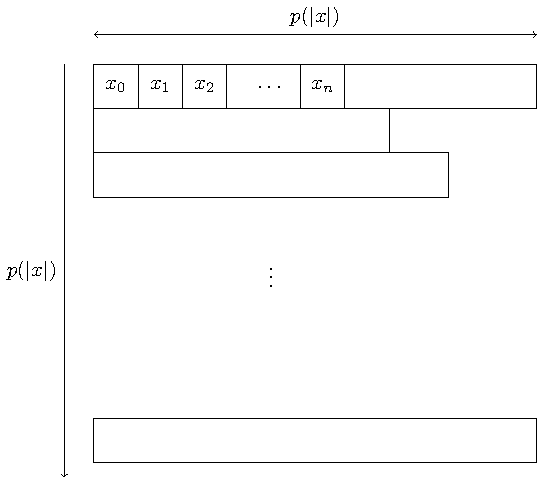
\includegraphics{./img/nondeterminism/SATproof1.pdf}
            \caption{Possiamo descrivere le possibili computazioni di una MdTN $M$ mediante una
            tabella cosi' fatta.}
        \end{center}
    \end{figure}

    Vogliamo descrivere questa matrice con una formula proposizionale. Questa matrice non e' unica,
    dato che esistono varie computazioni. La prima riga e' fissata alla configurazione iniziale, e
    l'ultima da quella finale. Lasciamo la liberta' alla matrice di rappresentare varie
    computazioni, dato che una riga non e' deterministicamente determinata da quella che la precede.

    %Slide 121

    Come rappresentiamo la matrice con una formula proposizionale?
    %Abbiamo a disposizione tutte le variabili che vogliamo.
    Usiamo delle variabili $y_{i,j,x}$. $i$ rappresenta il tempo (il passo $i$ della computazione),
    $j$ corrisponde alla cella, e $x$ al simbolo dell'alfabeto della matrice che sta nella cella $j$
    al tempo $i$.  La variabile e' vera se $x$ e' nella cella $j$ al tempo $i$, e falsa altrimenti.
    Vogliamo ora costruire un sistema di vincoli che corrisponde all'esistenza di una computazione
    accettante che utilizzi questo tipo di variabili. Per esprimere questi vincoli usiamo delle
    formule proposizionali.

    Definimao le ``cornici'' della matrice: prima e ultima configurazione, e i due lati della
    matrice. Possiamo supporre che il riconoscimento, se avviene, avvenga esattamente al momento
    $p(|x|)$. E' facile imporre questo vincolo anche su computazioni che accettano prima. L'alfabeto
    che stiamo considerando per questa matrice e' l'alfabeto $\Gamma' = \Gamma \cup (Q \times
    \Gamma)$, dove $\Gamma$ e' l'alfabeto di $M$ e la seconda parte codifica lo stato interno e la
    posizione della testina. Dove sta la coppia $q,x$ e' posizionata la testina. Inoltre abbiamo che
    lo stato interno e' $q$. Poiche' stiamo lavorando con un solo nastro ci aspettiamo che la
    testina sia su un solo carattere in ogni istante della computazione.

    Perche' vogliamo definire il bordo? Per semplicita'. E' abbastanza importante definirlo.
    %Supponiamo che $x = x_{1}\dotsc x_{n}$.
    Vogliamo che i bordi non siamo oltrepassati: li settiamo a blank e
    faremo in modo che rimangano blank per il resto della computazione.

    \begin{figure}[h]
        \begin{center}
            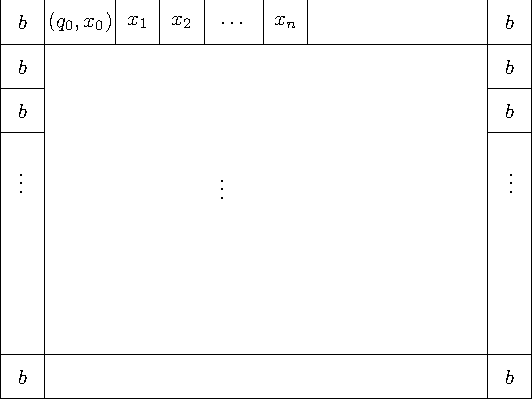
\includegraphics{./img/nondeterminism/SATproof2.pdf}
            \caption{Facciamo in modo che i bordi della tabella abbiano sempre il simbolo blank e
            che la prima riga corrisponda alla configurazione iniziale di $M$}
        \end{center}
    \end{figure}

    %Slide 122

    Possiamo iniziare a definire qualche vincolo. Vogliamo che ogni cella della matrice contenga uno ed
    un solo carattere. Questo vincolo e' espresso dalla seguente formula proposizionale:
    \begin{equation*}
        \phi_{0} = \bigwedge_{i=0}^{p(n)}\bigwedge_{j=0}^{p(n)}\left(\bigvee_{a \in \Gamma'}
            y_{i,j,a}
        \land \bigwedge_{a,b \in \Gamma',a \not= b}(\lnot y_{i,j,a} \lor \lnot y_{i,j,b})\right)
    \end{equation*}
    
    Per ogni istante di tempo da $i$ a $p(n)$, per ogni cella da $j$ a $p(n)$ almeno una delle
    variabili $y_{i,j,a}$ deve avere valore true. La dimensione della formula e' quadratica, ma per
    noi va bene perche' e' polinomiale. Vogliamo che tutte queste formule siano polinomiali in
    dimensione. La seconda parte del vincolo corrisponde a esprimere il fatto che vogliamo che una
    sola variabile abbia valore true tra le varie $y_{i,j,a}$ con $i$ e $j$ fissati.

    Questo vincolo e' un vincolo di ``soundness'' sulla matrice. Vogliamo ora esprimere il vincolo che
    sui bordi ci siano i caratteri blank. Questo e' espresso dalla seguente formula:
    \begin{equation*}
        \phi_{1} = \bigwedge_{i=0}^{p(n)}(y_{i,0,B} \land y_{i,p(n)+1,B})
    \end{equation*}

    Vogliamo fissare la configurazione iniziale e quella finale. Sappiamo com'e' fatta la configurazione
    iniziale, ed esprimiamo il vincolo che la matrice esprima quella configurazione nella prima riga con
    la seguente formula:
    \begin{equation*}
        \phi_{2} = y_{0,1,(q_{0},x_{0})} \land \bigwedge_{j=2}^{n}(y_{0,j,x_{j}}) \land
        \bigwedge_{j=n+1}^{p(n)}y_{i,j,B}
    \end{equation*}

    Ci aspettiamo che il carattere 0 sia $(q,x_{0})$, che nelle restanti celle ci siano i simboli
    dell'input, e che tutte le celle da $n$ in poi siano blank.

    Ci aspettiamo poi che l'ultima riga della matrice sia una configurazione di accettazione.
    Vogliamo ovvero che corrisponda ad una configurazione finale, ovvero che da qualche parte sul
    nastro la testina si sia arrestata in uno stato di accettazione. In termini della matrica ci
    aspettiamo che nell'ultima riga ci sia una cella con un carattere $F \times \Gamma$, dove $F$
    rappresenta il sottoinsieme di $Q$ di stati accettanti. Questo e' espresso dalla seguente
    formula:
    \begin{equation*}
        \phi_{3} = \bigvee_{j={1}}^{p(n)}\bigvee_{a \in F \times \Gamma}(y_{p(n),j,a})
    \end{equation*}

    Ci resta da descrivere la parte interna della matrice. In che modo vogliamo descrivere questa
    matrice? Come saranno fatte due righe successive? Saranno quasi identiche, dato che sono due
    configurazioni successive della computazione di $M$. Il nastro, durante un passo di
    computazione, cambia poco, dato che le operazioni tipiche di una MdT sono la scrittura di un
    carattere, lo spostamento della testina e il cambio del proprio stato interno. Supponiamo che la
    testina sia un una posizione $j$ con stato $q$ e carattere $a$. Cosa rimarra' sicuramente
    indentico nella riga successiva? Tutte le celle prima la cella $j-1$ e tutte le celle successive
    alla $j+1$. Al piu' cambiano 6 celle, in base alla riscrittura del carattere e al movimento
    della testina. 

    \begin{figure}[h]
        \begin{center}
            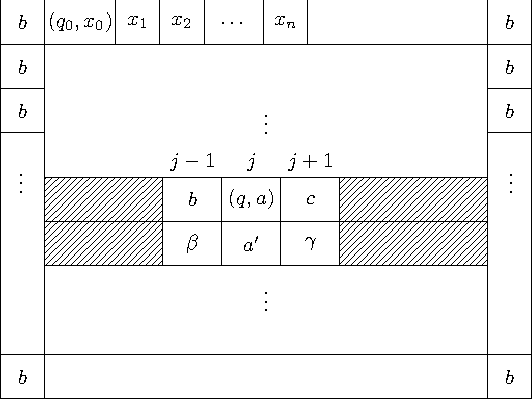
\includegraphics{./img/nondeterminism/SATproof3.pdf}
            \caption{Le uniche celle che cambiano durante un passo di computazione sono le 6 celle
                che comprendono quella con la testina e le altre 5 adiacenti. Avremo che $\beta = b$ e
                $\gamma = (q,c)$ se la testina si muove a destra, oppure $\beta = (q,b)$ e $\gamma = c$
            se la testina si muove a sinistra}
        \end{center}
    \end{figure}
    %Slide 123

    Esprimiamo questo con la seguente formula:
    \begin{equation*}
        \phi_{4} = \bigwedge_{i=0}^{p(n)-1}\bigwedge_{j=1}^{p(n)}\bigwedge_{a,b,c\in \Gamma}
        (y_{i,j-1,a} \land y_{i,j,b} \land y_{i,j+1,c} \implies y_{i+1,j,b})
    \end{equation*}
    Sappiamo che, se su una cella $j$ non c'e la testina e la testina non e' ne' nella cella $j-1$
    ne' in quella $j+1$ allora il carattere in $j$ non cambia.  Questo vale per tutte le celle.

    Finora non abbiamo usato molto della Macchina di Turing. Queste condizioni dipendenvano
    dall'alfabeto della macchina, dagli stati e dall'input. Quello che vogliamo ora esprimere
    dipende dalla funzione di transizione di $M$.

    La seguente formula richiede che per tutte le celle prima dell'ultima riga valga una certa
    formula $\Delta$, che andiamo a definire, e che dipende anche dai simboli di $Q \times F$:
    \begin{equation*}
        \phi_{5} = \bigwedge_{i=0}^{p(n)-1}\bigwedge_{j=1}^{p(n)}\bigwedge_{(q,a)\in Q\times F}
        \Delta_{q,a,i,j}
    \end{equation*}

    %Slide 124

    $\Delta_{q,a,i,j}$ e' una formula implicativa. Supponiamo che al tempo $i$ in posizione $j$ ci
    sia la testina ed un carattere $a$, ovvero supponiamo che $y_{i,j,(q,a)}$ sia vera. Supponiamo
    inoltre che siano vere $y_{i,j-1,b}$ e $y_{i,j+1,c}$. Cosa possiamo dire di come sara' fatto il
    nastro al prossimo passo? Dipende dal programma. Consideriamo un caso particolare. Supponiamo
    che, con stato $q$ e carattere $a$, la funzione di transizione abbia due possibilita':
    \begin{equation*}
        \delta(q,a) = \set{(q',a',R),(q'',a'',L)}
    \end{equation*}
    In generale potremmo avere un numero finito diverso di possibilita'. Supponiamo che la macchina non
    deterministica scelga la prima strada. Ci aspettiamo allora che $y_{i+1,j-1,b} \land y_{i+1,j,a'}
    \land y_{i+1,j+1,(q',c)}$. Questa' e' una possibilita'. Ci aspetteremmo quindi che valga questa oppure
    $y_{i+1,j-1,(q'',b)},y_{i+1,j,a''},y_{i+1,j+1,c}$. In generale ci aspettiamo un or tra le
    possibilita'. 
    %Nel caso generale avremo un or tra tutte le possibilita'. 
    La formula $\Delta$ nel caso generale e' cosi' fatta:
    \begin{align*}
        \Delta_{q,a,i,j} &= \bigwedge_{b,c \in \Gamma}( y_{i,j-1,b} \land y_{i,j,(q,a)} \land
        y_{i,j+1,c} \\ &\implies \bigvee_{(q',a',M) \in \delta(q,a)}(y_{i+1,j-1,\beta_{M,q',b}} \land
        y_{i+1,j,a'} \land y_{i+1,j+1,\gamma_{M,q',c}}))
    \end{align*}
    dove
    \begin{equation*}
        \beta_{M,q',b} =
        \begin{cases}
            \case{(q',b)}{se $M = L$}\\
            \case{b}{altrimenti}\\
        \end{cases}
    \end{equation*}
    e
    \begin{equation*}
        \gamma_{M,q',c} =
        \begin{cases}
            \case{(q',c)}{se $M = R$}\\
            \case{c}{altrimenti}\\
        \end{cases}
    \end{equation*}

    Se c'e' una computazione accettante la formula $\phi_{x}^{M,p} = \phi_{0} \land \phi_{1} \land
    \phi_{2} \land \phi_{3} \land \phi_{4} \land \phi_{5}$ e' soddisfacibile. Viceversa se questa
    formula e' soddisfacibile allora $M$ era in grado di seguire una computazione che l'avrebbe
    portata al riconoscimento della stringa. Di conseguenza abbiamo che $A \leq_{p} SAT$. L'unico
    vincolo che abbiamo sul numero e sulla dimensione delle formule e' un vincolo di tipo
    polinomiale. Questa condizione e' pero' facilmente verificata. Questo conclude la dimostrazione.

\end{proof}

Con le formule proposizionali riusciamo a descrivere una cosa complessa come una computazione di una
MdTN. In generale con formule proposizionali possiamo esprimere e modellare molte cose, da cui le
tante riduzioni a $\SAT$ o $3\SAT$.

Quando abbiamo un problema $B$ $\NPClass$-completo e' interessante aggiungere vincoli per capire se
$B$ rimane $\NPClass$-completo. Ad esempio abbiamo visto che la 3-colorabilita' e'
$\NPClass$-completo, mentre la 2-colorabilita' e' in $\PClass$. A volte riusciamo ad aggiungere
abbastanza vincoli da restringerci da un problema $\NPClass$-completo ad un prolema in $\PClass$.

Sappiamo che le formule proposizionali possono essere espresse in delle forme normali. Le forme
normali tipiche sono la congiuntiva e disgiuntiva.  Una formula e' in forma normale congiuntiva
(Conjunctive normal form, CNF) se puo' essere espressa come una congiunzione di clausole, dove la
clausole sono disgiunzioni di letterali. Un letterale e' una variabile proposizionale o la sua
negata. Possiamo esprimere una clausola $A \land \lnot A \land C$ con una notazione insiemistica
come $\set{A,\lnot A,C}$. Questo perche' l'or e' idempotente: $A \lor A \equiv A$. Possiamo inoltre
rappresentare una conginzione di congiunzioni con una notazione insiemistica come ad esempio
$\set{\set{A,\lnot A,C},\set{A,\lnot B}}$.

Che vincoli possiamo immaginare di porre a $\SAT$? Possiamo immaginare di dare un vincolo al numero
di letterali nelle clausole. Se poniamo un vincolo di 3 letterali in ogni clausola otteniamo
$3\SAT$, l'insieme delle formule soddisfacibili espresse in CNF con clausole di 3 letterali.

Otteniamo in questo modo un problema piu' semplice di $\SAT$? Vedremo che in realta' no, poiche'
$\SAT \leq 3\SAT$.

\section{Riduzioni di problemi $\NPClass$-completi}

\subsection{$\SAT \leq 3\SAT$}

%Siamo ora interessati ad una ``restrizione'' di $\SAT$: $3\SAT$.

\begin{thm}
        $\SAT \leq 3\SAT$.
\end{thm}

Mostriamo ora che $3\SAT$ e' $\NPClass$-completo mostrando una riduzione da $\SAT$ a $3\SAT$. Per
fare cio' ci serve una trasformazione che richiede tempo polinomiale da formule generali a formule
in 3-CNF tale che conservi la soddisfacibilita' della formula.

Quando vogliamo facciamo una trasformazione di una formula di solito vogliamo ottenere una formula
equivalente a quella di partenza. In questo caso a noi interessa una cosa piu' debole: ottenere una
formula che sia soddisfacibile sse la formula di partenza era soddisfacibile.

Vediamo perche' non ci conviene usare una trasformazione che ci permtte di passare ad una formula
logicamente equivalente a quella di partenza. Data una qualsiasi formula della logica proposizionale
possiamo trasformarla in una logicamente equivalente in forma normale congiuntiva. Possiamo fare
questo perche' esistono varie equivalenze logiche notevoli che ci permettono di dare alla formula la
forma che desideriamo: ad esempio, $A \implies B \equiv \lnot A \lor B$.

Il primo passaggio e' trasformare tutti i connettivi nelle formule in loro corrispettivi equivalenti
espressi con $\lor,\land,\lnot$. Dopodiche' ``pushiamo'' le negazioni al piu' interno possibile nella
formula. Le regole che ci permettono di propagare la negazione all'interno della formula sono le
formule di de Morgan: ad esempio $\lnot (A \land B) \equiv \lnot A \lor \lnot B$. La propagazione
della negazione si blocca quando giungiamo alle formule atomiche. Abbiamo ancora un nesting
arbitrario di congiunzioni e disgiunzioni pero'. Questo puo' essere risolto utilizzando le regole di
distributivita': ad esempio, $A \lor (B \land C) \equiv (A \lor B) \land (A \lor C)$.

In questo modo possiamo ottenere una formula equivalente in 3-CNF. Abbiamo pero' un problema
abbastanza grave: in generale questa trasformazione puo' portare ad una esplosione esponenziale
della dimensione della formula. Questa trasformazione richiede quindi tempo esponenziale, e di
conseguenza non si tratta di una riduzione polinomiale.

Noi pero' siamo interessati alla soddisfacibilita'. Se non siamo interessati a preservare
l'equivalenza logica possiamo usare una trasformazione che conserva la soddisfacibilita' e che non
porta ad un'esplosione esponenziale.

Vediamo questa trasformazione con un esempio. Prendiamo la formula seguente:
\begin{equation}\label{eq:start}
    \bigwedge_{i=1}^{n}(x_{i}\land y_{i}) = (x_{1} \land y_{1}) \land \cdots \land (x_{n} \land y_{n})
\end{equation}

Se la trasformassimo in una formula equivalente utilizzando il metodo appena descritto otterremmo le
$2^{n}$ clausole:
\begin{equation*}
    \set{x_{1},\dotsc,x_{n-1},x_{n}},\set{x_{1},\dotsc,x_{n-1},y_{1}},\dotsc,\set{y_{1},\dotsc,y_{n-1},y_{n}}
\end{equation*}

Se invece passiamo dalla formula di partenza alla seguente, espressa come insieme di clausole:
\begin{equation}\label{eq:transformation}
    \set{z_{1},\dotsc,z_{n}},\set{\lnot z_{1},x_{1}},\set{\lnot z_{1},y_{1}},\dotsc,\set{\lnot
    z_{n},x_{n}},\set{\lnot z_{n},y_{n}}
\end{equation}
Otteniamo una formula soddisfacibile se e solo se lo era quella di partenza, ma che non e' ad essa
logicamente equivalente.  Inoltre la dimensione aumenta in modo lineare.  Ogni $z_{i}$ ci indica se
la coppia $x_{i} \land y_{i}$ era vera.

Se introduciamo variabili diverse due formule non possono essere equivalenti. Le equivalenze si
stabbiliscono tra formule con le stesse variabili.

Se la formula \ref{eq:transformation} e' vera almeno uno $z_{i}$ deve essere vero. In piu' tutte le
altre clausole devono essere vere. Dove $z_{i}$ e' vero sia $x_{i}$ che $y_{i}$ devono essere veri.
Ma allora era vera anche la formula \ref{eq:start}.

Adottando questa tecnica e' possibile dimostrare che ogni formula proposizionale puo' essere
trasformata in 3-CNF preservando la soddisfacibilita' con una crescita' al piu' polinomiale.

In generale non e' vero che possiamo trasformare una formula in una equivalente in CNF in tempo
polinomiale. Se siamo interessati alla soddisfacibilita' possiamo fare una trasformazione
polinomiale che ci restituisce una formula ``soddsifacibilmente equivalente'' a quella di partenza.
In particolare quest'ultima trasformazione non preserva la tautologicita' di una formula.

\subsection{$3\SAT \leq \VC$}

Vediamo ora un teorema abbastanza importante. E' un esempio interessante di riduzione. Vogliamo
dimostrare che $3\SAT$ e' riducibile a $\VC$.

\begin{thm}
        $3\SAT \leq \VC$
\end{thm}

Ricordiamo che $\VC$ e' il problema del ricoprimento di vertici:
\begin{equation*}
    \VC = \set{\pair{G}{k} \mid \text{Esiste un ricoprimento di vertici in $G$ di dimensione $\leq k$}}
\end{equation*}

Un ricoprimento di vertici e' un sottoinsieme $S$ di $V$ tale che per ogni arco uno dei nodi
dell'arco ricade in $S$.

Sono due problemi a priori diversi. Ci si potrebbe chiedere cosa abbia a che fare l'uno con l'altro.
Le riduzioni, in genere, mettono in relazione mondi diversi: ci permettono di vedere vari problemi
in modi diversi ma equivalenti.

La prima cosa da chiedersi quando si vuole fare una riduzione e' cosa richiedono in input il primo e
il secondo problema. $3\SAT$ richiede una formula $\varphi$ in 3-CNF e decide se questa e'
soddisfacibile o meno. Vertex Cover prende in input un grafo $G$ ed un intero $k$. La $f$ che
vogliamo costruire prende in input la formula $\varphi$ e restituisce in output una coppia
$\pair{G}{k}$. Inoltre vogliamo che $f \in \FP$.
\begin{equation*}
    \varphi \overset{f}{\mapsto} \pair{G}{k}
\end{equation*}

Dobbiamo inoltre dimostrare che $\varphi \in 3\SAT \iff \pair{G}{k} \in \VC$. La definizione di $f$
richiede del lavoro creativo.

Partiamo da un esempio. Supponiamo di avere una formula cosi' fatta:
\begin{equation*}
    \phi = \set{\set{A,\lnot B, C},\set{\lnot A, B \lnot C},\set{\lnot A,\lnot B, C},\set{A,B,\lnot
    C}}
\end{equation*}

Questa formula e' soddisfacibile. Se prendessimo la congiunzione di tutte le 8 possibili clausole la
formula sarebbe insoddisfacibile. E' facile verificare che qualsiasi sottoinsieme stretto delle
possibili clausole sarebbe soddisfacibile. Questo ci mostra che nonostante $3\SAT$ sia un problema
$\NPClass$-completo possono esistere delle euristiche che ci aiutano a capire se una formula e'
soddisfacibile o meno in maniera efficiente per certi casi particolari.

Da questa formula dobbiamo ottenere un grafo ed assegnargli un $k$. Il grafo $G$ e' fatto cosi':
\begin{itemize}
        \item Colleghiamo con un arco ogni letterale con il suo negato, creando un insieme di coppie
        \item Creiamo dei ``triangoli'' per ogni clausola
        \item Collegiamo i letterali tra di loro tra le coppie e i triangoli
\end{itemize}
La costruzione e' rappresentata nelle figure \ref{img:SATtoVC1} e \ref{img:SATtoVC2}

\begin{figure}[h]
    \begin{center}
        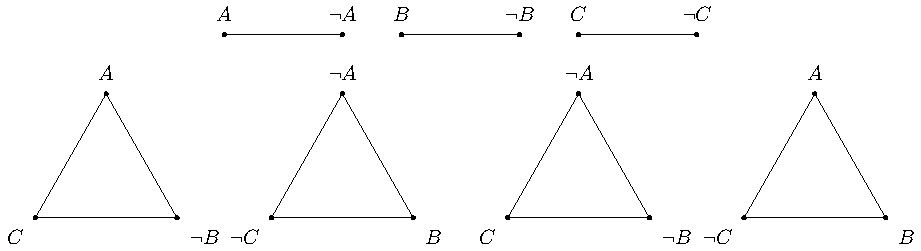
\includegraphics[scale=0.75]{./img/nondeterminism/SATtoVC1.pdf}
        \caption{Strutture di base del grafo $G$: coppie e triangoli}
        \label{img:SATtoVC1}
    \end{center}
\end{figure}

\begin{figure}[h]
    \begin{center}
        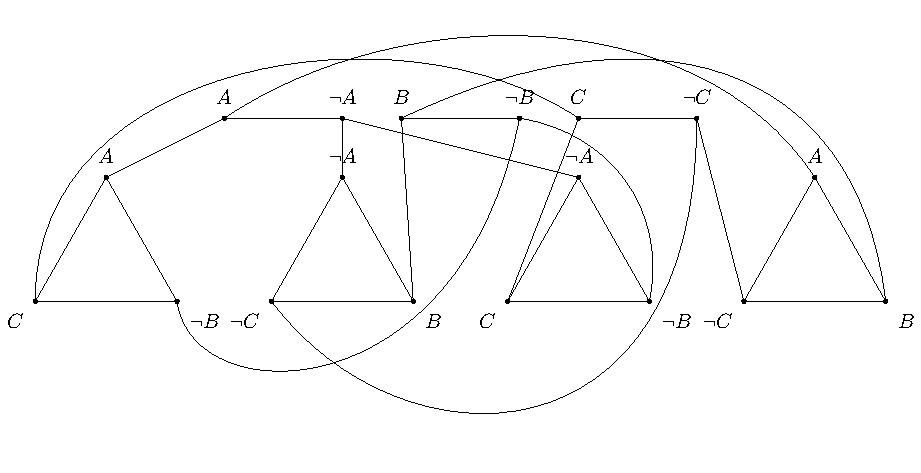
\includegraphics[scale=0.75]{./img/nondeterminism/SATtoVC2.pdf}
        \caption{Aggiunta degli archi tra i vertici del grafo}
        \label{img:SATtoVC2}
    \end{center}
\end{figure}

Quanti sono i nodi del grafo? Supponiamo che $n$ sia il numero delle variabili ed $m$ il numero
delle clausole. Per il nostro esempio $n=3$ e $m=4$. Abbiamo che il numero di nodi e' $2n + 3m$.

E' un grafo abbastanza sparso. Potremmo contare gli archi, ma e' abbastanza evidente che questi
siano in numero lineare nel numero dei nodi.

Quanti nodi dobbiamo prendere per coprire tutti gli archi? Per i triangoli almeno 2; per le coppie
almeno 1. Un ricoprimento deve avere una dimensione minima $2m + n$. Questo sara' il nostro $k$
della riduzione. Abbiamo quindi la nostra trasformazione $f$. Vogliamo dimostrare che se questo
grafo ha un ricoprimento di cardinalita' $\leq k$ la formula di partenza e' soddisfacibile, e
viceversa.

Mostriamo i due versi del sse, che sono abbastanza diversi.

Supponiamo che $\varphi$ sia soddisfacibile. Esiste quindi un'assegnamento di valori di verita' che
rende la formula soddisfacibile. Nel nostro esempio andrebbe bene l'assegnamento che assegna falso a
tutte le variabili proposizionali. Nel nostro grafo nelle coppie scegliamo per il ricoprimento il
letterale che, in base all'assegnemento, ha valore vero. In questo caso prenderemmo $\lnot A, \lnot
B, \lnot C$. Nei triangoli delle clausole abbiamo che c'e' un letterale direttamente collegato ad
uno dei letterali gia' scelti. Ad esempio, nel primo triangolo abbiamo che $\lnot B$ e' collegato al
corrispondente nella seconda coppia. Questo arco tra i due $\lnot B$ e' gia coperto. Di conseguenza
scegliamo per il ricoprimento gli altri due nodi. Facciamo questo per ogni clasuola. Quello che
otteniamo e' un ricoprimento su $G$ di dimensione $2m + n$. Quindi se $\varphi$ e' soddisfacibile
esiste un ricoprimento di dimensione $\leq k$.

Prendiamo ora il verso opposto. Supponiamo esista un ricoprimento di dimensione $2m + n$. Se abbiamo
un tale ricoprimento abbiamo che per ogni triangolo abbiamo preso almeno due vertici e per ogni
coppia abbiamo preso uno dei vertici. Per l'assegnamento dei valori di verita' assegnamo valore vero
ai vertici presi dalle coppie. Abbiamo che uno dei nodi, per ogni triangolo, deve toccare uno dei
nodi che abbiamo selezionato nelle coppie. Di conseguenza tale assegnamento di valori di verita'
soddisfa la formula. Di conseguenza se esiste un ricoprimento di dimensione $2m + n$ abbiamo che la
$\varphi$ corrispondente e' soddisfacibile.

\begin{figure}[h]
    \begin{center}
        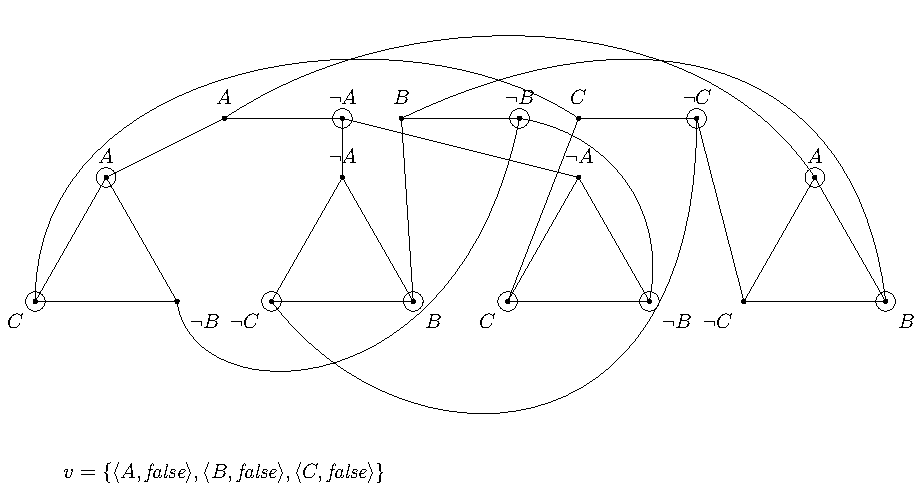
\includegraphics[scale=0.75]{./img/nondeterminism/SATtoVC3.pdf}
        \caption{I nodi cerchiati nel grafo $G$ fanno parte del sottoinsieme $S$ di copertura dei
        vertici}
    \end{center}
\end{figure}

Questo ci mostra, nuovamente, quanto siano importanti i grafi in informatica: sono una struttura
dati flessibile che ci permette di modellare molti problemi. Molti di questi possono essere espressi
come problemi di visita su grafi.

Abbiamo gia' visto che $\VC$ e' equivalente al problema della cricca e al problema dell'insieme
indipendente. Di conseguenza, poiche' abbiamo che $\VC$ e' $\NPClass$-completo per la dimostrazione
appena vista, abbiamo che anche cricca e insieme indipendente sono problemi $\NPClass$-completi.

\subsection{$\HAMPATH \equiv \HAMCYCLE$}

Vediamo una riduzione dal problema del cammino hamiltoniamo al ciclo hamiltoniano e una riduzione
inversa. Questi due problemi sono equivalenti.

Quello che vogliamo per ridurre il cammino hamiltioniano al ciclo hamiltoniano e' una riduzione tra
grafi che ci porti dal problema dell'esistenza di un cammino hamiltioniano al problema
dell'esistenza di un ciclo hamiltoniano.

Quello che facciamo e' aggiungere un nodo collegato a tutti i nodi del grafo $G$ di partenza.

\begin{figure}[h]
    \begin{center}
        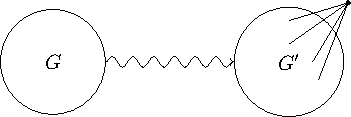
\includegraphics{./img/nondeterminism/HAMPATHCYCLE.pdf}
        \caption{Aggiungendo un nodo collegato a tutti gli altri trasformiamo un qualsiasi cammino
        hamiltoniano esistente in $G$ in un circuito che passa per il nuovo nodo}
    \end{center}
\end{figure}

Se abbiamo un cammino hamiltoniano in $G$ otteniamo un ciclo in $G'$ passando per il nuovo nuovo $n$
aggiunto dall'ultimo nodo del cammino e passando al primo nodo del cammino. Viceversa, se abbiamo un
ciclo in $G'$ questo include necessariamente $n$. Togliendo $n$ dal ciclo otteniamo un cammino
hamiltoniano in $G$.

L'altro verso e' piu' complesso. Non basta l'identita' come trasformazione perche' con questa non
vale il sse. L'identita' serve in genere a ridurre un problema a se stesso.

L'idea e' la seguente: partendo dal grafo selezioniamo un nodo arbitrario $n$. Questo nodo avra' un
po' di connessioni con altri nodi. Costruiamo una copia di questo nodo: aggiungiamo un nodo nuovo
$n'$ collegato a tutti i nodi a cui era collegato $n$. Aggiungiamo poi due nuovi nodi $m,m'$
collegati, rispettivamente, a $n$ e $n'$.

Il grafo $G'$ cosi' costruito a partire da $G$ ha un cammino hamiltoniano sse $G$ aveva un ciclo
hamiltoniano. Infatti sia $n$ il nodo che viene ``clonato'' in $G$ e sia $p = n_{1}, \dotsc,
n_{i-1}, n, n_{i}, \dotsc, n_{n}, n_{1}$ un ciclo hamiltoniano in $G$. In $G'$ costruiamo un cammino
hamiltoniano a partire da $p$ nel seguente modo: partiamo da $m$, passiamo per $n$, e seguiamo $p$
in un qualche verso. Ad esempio da $n$ passiamo a $n_{i}$ fino a tornare a $n_{i-1}$. A questo punto
da $n_{i-1}$ passiamo al nodo clone $n'$ e da li' passiamo infine ad $m'$. Possiamo passare da
$n_{i-1}$ a $n'$ poiche' $n'$ e' collegato a tutti i nodi adiacenti ad $n$, e $n_{i-1}$ e' adiacente
ad $n$.

Viceversa, se in $G'$ abbiamo un cammino hamiltoniano allora abbiamo un circuito hamiltoniano in
$G$. Infatti se esiste un cammino hamiltoniano $p'$ questo deve necessariamente avere come estremi
del cammino $m$ e $m'$. Sia, ad esempio, $p' = m, n, n_{i},\dotsc, n_{i-1}, n', m'$. Da $p'$
possiamo ottenere un ciclo hamiltoniano in $G$ nel seguente modo: da $p'$ rimuoviamo $m, n'$ e $m'$
e aggiungiamo $n$ in fondo per chiudere il circuito. Siamo sicuri che questo sia un circuito
hamiltoniano in $G$ poiche' se $n_{i-1}$ era adiacente a $n'$ allora necessariamente era adiacente
anche ad $n$.

Illustriamo questa trasformazione con l'esempio in figura \ref{img:HAMCYCLEPATH}.

\begin{figure}[h]
    \begin{center}
        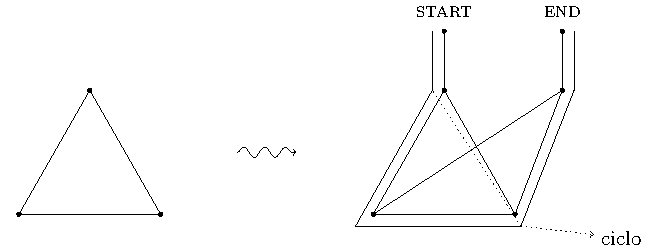
\includegraphics{./img/nondeterminism/HAMCYCLEPATH.pdf}
        \caption{Da un ciclo hamiltoniano in $G$ passiamo ad un cammino hamiltoniano in $G'$ e,
        viceversa, da un cammino hamiltoniano in $G'$ passiamo ad un ciclo in $G$}
        \label{img:HAMCYCLEPATH}
    \end{center}
\end{figure}

%Esercizio per la prossima volta. Prendiamo il problema del cammino ed il problema del cammino
%puntato. Il problema del cammino prende un grafo. Il problema del cammino puntato prende un grafo e
%due nodi. Il primo cerca di capire se esiste un cammino hamiltoniano. Il secondo cerca di capire se
%esiste un cammino hamiltoniano che parte dal primo nodo al secondo. Quest'ultimo semrerebbe piu'
%semplice. In realta' rimane NP-completo. Dimostrare una riduzione da CAM a CAM PUNTATO.

%
%\appendix
%\input{./tex/myappendix.tex}
%
%
% Bibliography:
%\clearpage
%\input{./tex/mybibliography.tex}

\end{document}
